\documentclass[twoside]{book}

% Packages required by doxygen
\usepackage{fixltx2e}
\usepackage{calc}
\usepackage{doxygen}
\usepackage[export]{adjustbox} % also loads graphicx
\usepackage{graphicx}
\usepackage[utf8]{inputenc}
\usepackage{makeidx}
\usepackage{multicol}
\usepackage{multirow}
\PassOptionsToPackage{warn}{textcomp}
\usepackage{textcomp}
\usepackage[nointegrals]{wasysym}
\usepackage[table]{xcolor}

% Font selection
\usepackage[T1]{fontenc}
\usepackage[scaled=.90]{helvet}
\usepackage{courier}
\usepackage{amssymb}
\usepackage{sectsty}
\renewcommand{\familydefault}{\sfdefault}
\allsectionsfont{%
  \fontseries{bc}\selectfont%
  \color{darkgray}%
}
\renewcommand{\DoxyLabelFont}{%
  \fontseries{bc}\selectfont%
  \color{darkgray}%
}
\newcommand{\+}{\discretionary{\mbox{\scriptsize$\hookleftarrow$}}{}{}}

% Page & text layout
\usepackage{geometry}
\geometry{%
  a4paper,%
  top=2.5cm,%
  bottom=2.5cm,%
  left=2.5cm,%
  right=2.5cm%
}
\tolerance=750
\hfuzz=15pt
\hbadness=750
\setlength{\emergencystretch}{15pt}
\setlength{\parindent}{0cm}
\setlength{\parskip}{3ex plus 2ex minus 2ex}
\makeatletter
\renewcommand{\paragraph}{%
  \@startsection{paragraph}{4}{0ex}{-1.0ex}{1.0ex}{%
    \normalfont\normalsize\bfseries\SS@parafont%
  }%
}
\renewcommand{\subparagraph}{%
  \@startsection{subparagraph}{5}{0ex}{-1.0ex}{1.0ex}{%
    \normalfont\normalsize\bfseries\SS@subparafont%
  }%
}
\makeatother

% Headers & footers
\usepackage{fancyhdr}
\pagestyle{fancyplain}
\fancyhead[LE]{\fancyplain{}{\bfseries\thepage}}
\fancyhead[CE]{\fancyplain{}{}}
\fancyhead[RE]{\fancyplain{}{\bfseries\leftmark}}
\fancyhead[LO]{\fancyplain{}{\bfseries\rightmark}}
\fancyhead[CO]{\fancyplain{}{}}
\fancyhead[RO]{\fancyplain{}{\bfseries\thepage}}
\fancyfoot[LE]{\fancyplain{}{}}
\fancyfoot[CE]{\fancyplain{}{}}
\fancyfoot[RE]{\fancyplain{}{\bfseries\scriptsize Generated by Doxygen }}
\fancyfoot[LO]{\fancyplain{}{\bfseries\scriptsize Generated by Doxygen }}
\fancyfoot[CO]{\fancyplain{}{}}
\fancyfoot[RO]{\fancyplain{}{}}
\renewcommand{\footrulewidth}{0.4pt}
\renewcommand{\chaptermark}[1]{%
  \markboth{#1}{}%
}
\renewcommand{\sectionmark}[1]{%
  \markright{\thesection\ #1}%
}

% Indices & bibliography
\usepackage{natbib}
\usepackage[titles]{tocloft}
\setcounter{tocdepth}{3}
\setcounter{secnumdepth}{5}
\makeindex

% Packages requested by user
\usepackage{amsmath}

% Hyperlinks (required, but should be loaded last)
\usepackage{ifpdf}
\ifpdf
  \usepackage[pdftex,pagebackref=true]{hyperref}
\else
  \usepackage[ps2pdf,pagebackref=true]{hyperref}
\fi
\hypersetup{%
  colorlinks=true,%
  linkcolor=blue,%
  citecolor=blue,%
  unicode%
}

% Custom commands
\newcommand{\clearemptydoublepage}{%
  \newpage{\pagestyle{empty}\cleardoublepage}%
}

\usepackage{caption}
\captionsetup{labelsep=space,justification=centering,font={bf},singlelinecheck=off,skip=4pt,position=top}

%===== C O N T E N T S =====

\begin{document}

% Titlepage & ToC
\hypersetup{pageanchor=false,
             bookmarksnumbered=true,
             pdfencoding=unicode
            }
\pagenumbering{roman}
\begin{titlepage}
\vspace*{7cm}
\begin{center}%
{\Large Biogeme\+: Python Library }\\
\vspace*{1cm}
{\large Generated by Doxygen 1.8.11}\\
\end{center}
\end{titlepage}
\clearemptydoublepage
\tableofcontents
\clearemptydoublepage
\pagenumbering{arabic}
\hypersetup{pageanchor=true}

%--- Begin generated contents ---
\chapter{Module Index}
\section{Modules}
Here is a list of all modules\+:\begin{DoxyCompactList}
\item \contentsline{section}{Specific choice models}{\pageref{group__models}}{}
\item \contentsline{section}{Functions helping to write the log likelihood function}{\pageref{group__likelihood}}{}
\item \contentsline{section}{pdf and C\+DF of common distributions}{\pageref{group__pdfcdf}}{}
\item \contentsline{section}{Functions calculating statistics on the sample}{\pageref{group__stats}}{}
\item \contentsline{section}{Functions used for the model specification}{\pageref{group__specs}}{}
\end{DoxyCompactList}

\chapter{Namespace Index}
\section{Packages}
Here are the packages with brief descriptions (if available)\+:\begin{DoxyCompactList}
\item\contentsline{section}{\hyperlink{namespacebiogeme}{biogeme} }{\pageref{namespacebiogeme}}{}
\end{DoxyCompactList}

\chapter{Hierarchical Index}
\section{Class Hierarchy}
This inheritance list is sorted roughly, but not completely, alphabetically\+:\begin{DoxyCompactList}
\item \contentsline{section}{biogeme.\+B\+I\+O\+G\+E\+M\+E\+\_\+\+O\+B\+J\+E\+CT}{\pageref{classbiogeme_1_1_b_i_o_g_e_m_e___o_b_j_e_c_t}}{}
\item \contentsline{section}{bio\+\_\+expression.\+Expression}{\pageref{classbio__expression_1_1_expression}}{}
\begin{DoxyCompactList}
\item \contentsline{section}{bio\+\_\+expression.\+abs}{\pageref{classbio__expression_1_1abs}}{}
\item \contentsline{section}{bio\+\_\+expression.\+Beta}{\pageref{classbio__expression_1_1_beta}}{}
\item \contentsline{section}{bio\+\_\+expression.\+Bin\+Op}{\pageref{classbio__expression_1_1_bin_op}}{}
\item \contentsline{section}{bio\+\_\+expression.\+bio\+Bayes\+Normal\+Draw}{\pageref{classbio__expression_1_1bio_bayes_normal_draw}}{}
\item \contentsline{section}{bio\+\_\+expression.\+bio\+Draws}{\pageref{classbio__expression_1_1bio_draws}}{}
\item \contentsline{section}{bio\+\_\+expression.\+bio\+Logit}{\pageref{classbio__expression_1_1bio_logit}}{}
\item \contentsline{section}{bio\+\_\+expression.\+bio\+Log\+Logit}{\pageref{classbio__expression_1_1bio_log_logit}}{}
\item \contentsline{section}{bio\+\_\+expression.\+bio\+Mult\+Sum}{\pageref{classbio__expression_1_1bio_mult_sum}}{}
\item \contentsline{section}{bio\+\_\+expression.\+bio\+Normal\+Cdf}{\pageref{classbio__expression_1_1bio_normal_cdf}}{}
\item \contentsline{section}{bio\+\_\+expression.\+bio\+Normal\+Draws}{\pageref{classbio__expression_1_1bio_normal_draws}}{}
\item \contentsline{section}{bio\+\_\+expression.\+bio\+Normal\+Pdf}{\pageref{classbio__expression_1_1bio_normal_pdf}}{}
\item \contentsline{section}{bio\+\_\+expression.\+bio\+Recycle\+Draws}{\pageref{classbio__expression_1_1bio_recycle_draws}}{}
\item \contentsline{section}{bio\+\_\+expression.\+bio\+Uniform\+Draws}{\pageref{classbio__expression_1_1bio_uniform_draws}}{}
\item \contentsline{section}{bio\+\_\+expression.\+bio\+Uniform\+Symmetric\+Draws}{\pageref{classbio__expression_1_1bio_uniform_symmetric_draws}}{}
\item \contentsline{section}{bio\+\_\+expression.\+Define\+Draws}{\pageref{classbio__expression_1_1_define_draws}}{}
\item \contentsline{section}{bio\+\_\+expression.\+Define\+Variable}{\pageref{classbio__expression_1_1_define_variable}}{}
\item \contentsline{section}{bio\+\_\+expression.\+Derive}{\pageref{classbio__expression_1_1_derive}}{}
\item \contentsline{section}{bio\+\_\+expression.\+Elem}{\pageref{classbio__expression_1_1_elem}}{}
\item \contentsline{section}{bio\+\_\+expression.\+Enumerate}{\pageref{classbio__expression_1_1_enumerate}}{}
\item \contentsline{section}{bio\+\_\+expression.\+exp}{\pageref{classbio__expression_1_1exp}}{}
\item \contentsline{section}{bio\+\_\+expression.\+Integrate}{\pageref{classbio__expression_1_1_integrate}}{}
\item \contentsline{section}{bio\+\_\+expression.\+log}{\pageref{classbio__expression_1_1log}}{}
\item \contentsline{section}{bio\+\_\+expression.\+max}{\pageref{classbio__expression_1_1max}}{}
\item \contentsline{section}{bio\+\_\+expression.\+MH}{\pageref{classbio__expression_1_1_m_h}}{}
\item \contentsline{section}{bio\+\_\+expression.\+min}{\pageref{classbio__expression_1_1min}}{}
\item \contentsline{section}{bio\+\_\+expression.\+Monte\+Carlo}{\pageref{classbio__expression_1_1_monte_carlo}}{}
\item \contentsline{section}{bio\+\_\+expression.\+Monte\+Carlo\+Control\+Variate}{\pageref{classbio__expression_1_1_monte_carlo_control_variate}}{}
\item \contentsline{section}{bio\+\_\+expression.\+Numeric}{\pageref{classbio__expression_1_1_numeric}}{}
\item \contentsline{section}{bio\+\_\+expression.\+Prod}{\pageref{classbio__expression_1_1_prod}}{}
\item \contentsline{section}{bio\+\_\+expression.\+Random\+Variable}{\pageref{classbio__expression_1_1_random_variable}}{}
\item \contentsline{section}{bio\+\_\+expression.\+Sum}{\pageref{classbio__expression_1_1_sum}}{}
\item \contentsline{section}{bio\+\_\+expression.\+Un\+Op}{\pageref{classbio__expression_1_1_un_op}}{}
\item \contentsline{section}{bio\+\_\+expression.\+Variable}{\pageref{classbio__expression_1_1_variable}}{}
\end{DoxyCompactList}
\item \contentsline{section}{bio\+\_\+iterator.\+iterator}{\pageref{classbio__iterator_1_1iterator}}{}
\begin{DoxyCompactList}
\item \contentsline{section}{bio\+\_\+iterator.\+draw\+Iterator}{\pageref{classbio__iterator_1_1draw_iterator}}{}
\item \contentsline{section}{bio\+\_\+iterator.\+meta\+Iterator}{\pageref{classbio__iterator_1_1meta_iterator}}{}
\item \contentsline{section}{bio\+\_\+iterator.\+row\+Iterator}{\pageref{classbio__iterator_1_1row_iterator}}{}
\end{DoxyCompactList}
\item object\begin{DoxyCompactList}
\item \contentsline{section}{bio\+Matrix.\+bio\+Matrix}{\pageref{classbio_matrix_1_1bio_matrix}}{}
\end{DoxyCompactList}
\item \contentsline{section}{bio\+\_\+expression.\+Operator}{\pageref{classbio__expression_1_1_operator}}{}
\item \contentsline{section}{biogeme.\+S\+T\+AN}{\pageref{classbiogeme_1_1_s_t_a_n}}{}
\end{DoxyCompactList}

\chapter{Class Index}
\section{Class List}
Here are the classes, structs, unions and interfaces with brief descriptions\+:\begin{DoxyCompactList}
\item\contentsline{section}{\hyperlink{class____iterator__panel_obs_iter}{\+\_\+\+\_\+iterator\+\_\+panel\+Obs\+Iter} }{\pageref{class____iterator__panel_obs_iter}}{}
\item\contentsline{section}{\hyperlink{classbio_arith_abs}{bio\+Arith\+Abs} }{\pageref{classbio_arith_abs}}{}
\item\contentsline{section}{\hyperlink{classbio_arith_and}{bio\+Arith\+And} }{\pageref{classbio_arith_and}}{}
\item\contentsline{section}{\hyperlink{classbio_arith_bayes}{bio\+Arith\+Bayes} }{\pageref{classbio_arith_bayes}}{}
\item\contentsline{section}{\hyperlink{classbio_arith_bayes_mean}{bio\+Arith\+Bayes\+Mean} }{\pageref{classbio_arith_bayes_mean}}{}
\item\contentsline{section}{\hyperlink{classbio_arith_bayes_m_h}{bio\+Arith\+Bayes\+MH} }{\pageref{classbio_arith_bayes_m_h}}{}
\item\contentsline{section}{\hyperlink{classbio_arith_binary_expression}{bio\+Arith\+Binary\+Expression} }{\pageref{classbio_arith_binary_expression}}{}
\item\contentsline{section}{\hyperlink{classbio_arith_binary_minus}{bio\+Arith\+Binary\+Minus} }{\pageref{classbio_arith_binary_minus}}{}
\item\contentsline{section}{\hyperlink{classbio_arith_binary_plus}{bio\+Arith\+Binary\+Plus} }{\pageref{classbio_arith_binary_plus}}{}
\item\contentsline{section}{\hyperlink{classbio_arith_composite_literal}{bio\+Arith\+Composite\+Literal} }{\pageref{classbio_arith_composite_literal}}{}
\item\contentsline{section}{\hyperlink{classbio_arith_constant}{bio\+Arith\+Constant} }{\pageref{classbio_arith_constant}}{}
\item\contentsline{section}{\hyperlink{classbio_arith_derivative}{bio\+Arith\+Derivative} }{\pageref{classbio_arith_derivative}}{}
\item\contentsline{section}{\hyperlink{classbio_arith_divide}{bio\+Arith\+Divide} }{\pageref{classbio_arith_divide}}{}
\item\contentsline{section}{\hyperlink{classbio_arith_elem}{bio\+Arith\+Elem} }{\pageref{classbio_arith_elem}}{}
\item\contentsline{section}{\hyperlink{classbio_arith_elementary_expression}{bio\+Arith\+Elementary\+Expression} }{\pageref{classbio_arith_elementary_expression}}{}
\item\contentsline{section}{\hyperlink{classbio_arith_equal}{bio\+Arith\+Equal} }{\pageref{classbio_arith_equal}}{}
\item\contentsline{section}{\hyperlink{classbio_arith_exp}{bio\+Arith\+Exp} }{\pageref{classbio_arith_exp}}{}
\item\contentsline{section}{\hyperlink{classbio_arith_fixed_parameter}{bio\+Arith\+Fixed\+Parameter} }{\pageref{classbio_arith_fixed_parameter}}{}
\item\contentsline{section}{\hyperlink{classbio_arith_gauss_hermite}{bio\+Arith\+Gauss\+Hermite} }{\pageref{classbio_arith_gauss_hermite}}{}
\item\contentsline{section}{\hyperlink{classbio_arith_g_h_integral}{bio\+Arith\+G\+H\+Integral} }{\pageref{classbio_arith_g_h_integral}}{}
\item\contentsline{section}{\hyperlink{classbio_arith_greater}{bio\+Arith\+Greater} }{\pageref{classbio_arith_greater}}{}
\item\contentsline{section}{\hyperlink{classbio_arith_greater_equal}{bio\+Arith\+Greater\+Equal} }{\pageref{classbio_arith_greater_equal}}{}
\item\contentsline{section}{\hyperlink{classbio_arith_integral}{bio\+Arith\+Integral} }{\pageref{classbio_arith_integral}}{}
\item\contentsline{section}{\hyperlink{classbio_arith_iterator}{bio\+Arith\+Iterator} }{\pageref{classbio_arith_iterator}}{}
\item\contentsline{section}{\hyperlink{classbio_arith_less}{bio\+Arith\+Less} }{\pageref{classbio_arith_less}}{}
\item\contentsline{section}{\hyperlink{classbio_arith_less_equal}{bio\+Arith\+Less\+Equal} }{\pageref{classbio_arith_less_equal}}{}
\item\contentsline{section}{\hyperlink{classbio_arith_likelihood_fct_and_grad}{bio\+Arith\+Likelihood\+Fct\+And\+Grad} }{\pageref{classbio_arith_likelihood_fct_and_grad}}{}
\item\contentsline{section}{\hyperlink{classbio_arith_list_of_expressions}{bio\+Arith\+List\+Of\+Expressions} }{\pageref{classbio_arith_list_of_expressions}}{}
\item\contentsline{section}{\hyperlink{classbio_arith_literal}{bio\+Arith\+Literal} }{\pageref{classbio_arith_literal}}{}
\item\contentsline{section}{\hyperlink{classbio_arith_log}{bio\+Arith\+Log} }{\pageref{classbio_arith_log}}{}
\item\contentsline{section}{\hyperlink{classbio_arith_log_logit}{bio\+Arith\+Log\+Logit} }{\pageref{classbio_arith_log_logit}}{}
\item\contentsline{section}{\hyperlink{classbio_arith_matrix}{bio\+Arith\+Matrix} }{\pageref{classbio_arith_matrix}}{}
\item\contentsline{section}{\hyperlink{classbio_arith_max}{bio\+Arith\+Max} }{\pageref{classbio_arith_max}}{}
\item\contentsline{section}{\hyperlink{classbio_arith_min}{bio\+Arith\+Min} }{\pageref{classbio_arith_min}}{}
\item\contentsline{section}{\hyperlink{classbio_arith_monte_carlo}{bio\+Arith\+Monte\+Carlo} }{\pageref{classbio_arith_monte_carlo}}{}
\item\contentsline{section}{\hyperlink{classbio_arith_mult}{bio\+Arith\+Mult} }{\pageref{classbio_arith_mult}}{}
\item\contentsline{section}{\hyperlink{classbio_arith_multinary_expression}{bio\+Arith\+Multinary\+Expression} }{\pageref{classbio_arith_multinary_expression}}{}
\item\contentsline{section}{\hyperlink{classbio_arith_multinary_plus}{bio\+Arith\+Multinary\+Plus} }{\pageref{classbio_arith_multinary_plus}}{}
\item\contentsline{section}{\hyperlink{classbio_arith_normal_cdf}{bio\+Arith\+Normal\+Cdf} }{\pageref{classbio_arith_normal_cdf}}{}
\item\contentsline{section}{\hyperlink{classbio_arith_normal_pdf}{bio\+Arith\+Normal\+Pdf} }{\pageref{classbio_arith_normal_pdf}}{}
\item\contentsline{section}{\hyperlink{classbio_arith_not_equal}{bio\+Arith\+Not\+Equal} }{\pageref{classbio_arith_not_equal}}{}
\item\contentsline{section}{\hyperlink{classbio_arith_or}{bio\+Arith\+Or} }{\pageref{classbio_arith_or}}{}
\item\contentsline{section}{\hyperlink{classbio_arith_power}{bio\+Arith\+Power} }{\pageref{classbio_arith_power}}{}
\item\contentsline{section}{\hyperlink{classbio_arith_print}{bio\+Arith\+Print} }{\pageref{classbio_arith_print}}{}
\item\contentsline{section}{\hyperlink{classbio_arith_prod}{bio\+Arith\+Prod} }{\pageref{classbio_arith_prod}}{}
\item\contentsline{section}{\hyperlink{classbio_arith_random}{bio\+Arith\+Random} }{\pageref{classbio_arith_random}}{}
\item\contentsline{section}{\hyperlink{classbio_arith_random_variable}{bio\+Arith\+Random\+Variable} }{\pageref{classbio_arith_random_variable}}{}
\item\contentsline{section}{\hyperlink{classbio_arith_sum}{bio\+Arith\+Sum} }{\pageref{classbio_arith_sum}}{}
\item\contentsline{section}{\hyperlink{classbio_arith_unary_expression}{bio\+Arith\+Unary\+Expression} }{\pageref{classbio_arith_unary_expression}}{}
\item\contentsline{section}{\hyperlink{classbio_arith_unary_minus}{bio\+Arith\+Unary\+Minus} }{\pageref{classbio_arith_unary_minus}}{}
\item\contentsline{section}{\hyperlink{classbio_arith_unif_random}{bio\+Arith\+Unif\+Random} }{\pageref{classbio_arith_unif_random}}{}
\item\contentsline{section}{\hyperlink{classbio_arith_variable}{bio\+Arith\+Variable} }{\pageref{classbio_arith_variable}}{}
\item\contentsline{section}{\hyperlink{classbio_bayesian_results}{bio\+Bayesian\+Results} }{\pageref{classbio_bayesian_results}}{}
\item\contentsline{section}{\hyperlink{classbio_composite_literal}{bio\+Composite\+Literal} }{\pageref{classbio_composite_literal}}{}
\item\contentsline{section}{\hyperlink{classbio_constraints}{bio\+Constraints} }{\pageref{classbio_constraints}}{}
\item\contentsline{section}{\hyperlink{classbio_constraint_wrapper}{bio\+Constraint\+Wrapper} }{\pageref{classbio_constraint_wrapper}}{}
\item\contentsline{section}{\hyperlink{classbio_count_operations}{bio\+Count\+Operations} }{\pageref{classbio_count_operations}}{}
\item\contentsline{section}{\hyperlink{structbio_random_draws_1_1bio_draw}{bio\+Random\+Draws\+::bio\+Draw} }{\pageref{structbio_random_draws_1_1bio_draw}}{}
\item\contentsline{section}{\hyperlink{classbio_draw_iterator}{bio\+Draw\+Iterator} }{\pageref{classbio_draw_iterator}}{}
\item\contentsline{section}{\hyperlink{classbio_expression}{bio\+Expression} }{\pageref{classbio_expression}}{}
\item\contentsline{section}{\hyperlink{classbio_expression_repository}{bio\+Expression\+Repository} }{\pageref{classbio_expression_repository}}{}
\item\contentsline{section}{\hyperlink{classbio_fixed_parameter}{bio\+Fixed\+Parameter} }{\pageref{classbio_fixed_parameter}}{}
\item\contentsline{section}{\hyperlink{classbio_function_and_derivatives}{bio\+Function\+And\+Derivatives} }{\pageref{classbio_function_and_derivatives}}{}
\item\contentsline{section}{\hyperlink{structbio_gsl_params}{bio\+Gsl\+Params} }{\pageref{structbio_gsl_params}}{}
\item\contentsline{section}{\hyperlink{classbio_id_iterator}{bio\+Id\+Iterator} }{\pageref{classbio_id_iterator}}{}
\item\contentsline{section}{\hyperlink{classbio_iterates}{bio\+Iterates} }{\pageref{classbio_iterates}}{}
\item\contentsline{section}{\hyperlink{classbio_iteration_backup}{bio\+Iteration\+Backup} }{\pageref{classbio_iteration_backup}}{}
\item\contentsline{section}{\hyperlink{classbio_iterator}{bio\+Iterator$<$ T $>$} }{\pageref{classbio_iterator}}{}
\item\contentsline{section}{\hyperlink{classbio_iterator_info}{bio\+Iterator\+Info} }{\pageref{classbio_iterator_info}}{}
\item\contentsline{section}{\hyperlink{classbio_iterator_info_repository}{bio\+Iterator\+Info\+Repository} }{\pageref{classbio_iterator_info_repository}}{}
\item\contentsline{section}{\hyperlink{classbio_iterator_span}{bio\+Iterator\+Span} }{\pageref{classbio_iterator_span}}{}
\item\contentsline{section}{\hyperlink{classbio_literal}{bio\+Literal} }{\pageref{classbio_literal}}{}
\item\contentsline{section}{\hyperlink{classbio_literal_repository}{bio\+Literal\+Repository} }{\pageref{classbio_literal_repository}}{}
\item\contentsline{section}{\hyperlink{classbio_literal_values}{bio\+Literal\+Values} }{\pageref{classbio_literal_values}}{}
\item\contentsline{section}{\hyperlink{classbio_main}{bio\+Main} }{\pageref{classbio_main}}{}
\item\contentsline{section}{\hyperlink{classbio_meta_iterator}{bio\+Meta\+Iterator} }{\pageref{classbio_meta_iterator}}{}
\item\contentsline{section}{\hyperlink{classbio_minimization_problem}{bio\+Minimization\+Problem} }{\pageref{classbio_minimization_problem}}{}
\item\contentsline{section}{\hyperlink{classbio_model}{bio\+Model} }{\pageref{classbio_model}}{}
\item\contentsline{section}{\hyperlink{classbio_model_parser}{bio\+Model\+Parser} }{\pageref{classbio_model_parser}}{}
\item\contentsline{section}{\hyperlink{classbio_observation_data}{bio\+Observation\+Data} }{\pageref{classbio_observation_data}}{}
\item\contentsline{section}{\hyperlink{classbio_one_parameter}{bio\+One\+Parameter$<$ T $>$} }{\pageref{classbio_one_parameter}}{}
\item\contentsline{section}{\hyperlink{classbio_optimization_results}{bio\+Optimization\+Results} }{\pageref{classbio_optimization_results}}{}
\item\contentsline{section}{\hyperlink{classbio_parameter_iterator}{bio\+Parameter\+Iterator$<$ T $>$} }{\pageref{classbio_parameter_iterator}}{}
\item\contentsline{section}{\hyperlink{classbio_parameters}{bio\+Parameters} }{\pageref{classbio_parameters}}{}
\item\contentsline{section}{\hyperlink{classbio_precompiled_function}{bio\+Precompiled\+Function} }{\pageref{classbio_precompiled_function}}{}
\item\contentsline{section}{\hyperlink{classbio_premature_stop}{bio\+Premature\+Stop} }{\pageref{classbio_premature_stop}}{}
\item\contentsline{section}{\hyperlink{classbio_python_singleton_factory}{bio\+Python\+Singleton\+Factory} }{\pageref{classbio_python_singleton_factory}}{}
\item\contentsline{section}{\hyperlink{classbio_python_wrapper}{bio\+Python\+Wrapper} }{\pageref{classbio_python_wrapper}}{}
\item\contentsline{section}{\hyperlink{classbio_random_draws}{bio\+Random\+Draws} }{\pageref{classbio_random_draws}}{}
\item\contentsline{section}{\hyperlink{classbio_random_meta_iterator}{bio\+Random\+Meta\+Iterator} }{\pageref{classbio_random_meta_iterator}}{}
\item\contentsline{section}{\hyperlink{classbio_random_variable}{bio\+Random\+Variable} }{\pageref{classbio_random_variable}}{}
\item\contentsline{section}{\hyperlink{classbio_raw_results}{bio\+Raw\+Results} }{\pageref{classbio_raw_results}}{}
\item\contentsline{section}{\hyperlink{classbio_reporting}{bio\+Reporting} }{\pageref{classbio_reporting}}{}
\item\contentsline{section}{\hyperlink{classbio_row_iterator}{bio\+Row\+Iterator} }{\pageref{classbio_row_iterator}}{}
\item\contentsline{section}{\hyperlink{classbio_sample}{bio\+Sample} }{\pageref{classbio_sample}}{}
\item\contentsline{section}{\hyperlink{classbio_sensitivity_analysis}{bio\+Sensitivity\+Analysis} }{\pageref{classbio_sensitivity_analysis}}{}
\item\contentsline{section}{\hyperlink{classbio_simulated_values}{bio\+Simulated\+Values} }{\pageref{classbio_simulated_values}}{}
\item\contentsline{section}{\hyperlink{classbio_simulation}{bio\+Simulation} }{\pageref{classbio_simulation}}{}
\item\contentsline{section}{\hyperlink{classbio_split}{bio\+Split} }{\pageref{classbio_split}}{}
\item\contentsline{section}{\hyperlink{classbio_statistics}{bio\+Statistics} }{\pageref{classbio_statistics}}{}
\item\contentsline{section}{\hyperlink{structbio_thread_arg}{bio\+Thread\+Arg} }{\pageref{structbio_thread_arg}}{}
\item\contentsline{section}{\hyperlink{classbio_variable}{bio\+Variable} }{\pageref{classbio_variable}}{}
\item\contentsline{section}{\hyperlink{classbio_version}{bio\+Version} }{\pageref{classbio_version}}{}
\item\contentsline{section}{\hyperlink{classmy_bio_constraints}{my\+Bio\+Constraints} }{\pageref{classmy_bio_constraints}}{}
\item\contentsline{section}{\hyperlink{classmy_bio_statistics}{my\+Bio\+Statistics} }{\pageref{classmy_bio_statistics}}{}
\item\contentsline{section}{\hyperlink{structoperators__t}{operators\+\_\+t} }{\pageref{structoperators__t}}{}
\end{DoxyCompactList}

\chapter{File Index}
\section{File List}
Here is a list of all documented files with brief descriptions\+:\begin{DoxyCompactList}
\item\contentsline{section}{\hyperlink{bio__expression_8py}{bio\+\_\+expression.\+py} }{\pageref{bio__expression_8py}}{}
\item\contentsline{section}{\hyperlink{bio__iterator_8py}{bio\+\_\+iterator.\+py} }{\pageref{bio__iterator_8py}}{}
\item\contentsline{section}{{\bfseries biogeme-\/python3-\/config.\+py} }{\pageref{biogeme-python3-config_8py}}{}
\item\contentsline{section}{{\bfseries biogeme-\/python3.\+1-\/config.\+py} }{\pageref{biogeme-python3_81-config_8py}}{}
\item\contentsline{section}{{\bfseries biogeme-\/python3.\+2-\/config.\+py} }{\pageref{biogeme-python3_82-config_8py}}{}
\item\contentsline{section}{{\bfseries biogeme-\/python3.\+2-\/cygwin-\/config.\+py} }{\pageref{biogeme-python3_82-cygwin-config_8py}}{}
\item\contentsline{section}{{\bfseries biogeme-\/python3.\+3-\/config.\+py} }{\pageref{biogeme-python3_83-config_8py}}{}
\item\contentsline{section}{{\bfseries biogeme-\/python3.\+3m-\/config.\+py} }{\pageref{biogeme-python3_83m-config_8py}}{}
\item\contentsline{section}{{\bfseries biogeme-\/python3.\+4-\/config.\+py} }{\pageref{biogeme-python3_84-config_8py}}{}
\item\contentsline{section}{{\bfseries biogeme-\/python3.\+5-\/config.\+py} }{\pageref{biogeme-python3_85-config_8py}}{}
\item\contentsline{section}{{\bfseries biogeme.\+py} }{\pageref{biogeme_8py}}{}
\item\contentsline{section}{\hyperlink{bio_matrix_8py}{bio\+Matrix.\+py} }{\pageref{bio_matrix_8py}}{}
\item\contentsline{section}{\hyperlink{boxcox_8py}{boxcox.\+py} \\*Function implementing the Box-\/\+Cox transform of a variable }{\pageref{boxcox_8py}}{}
\item\contentsline{section}{\hyperlink{cnl_8py}{cnl.\+py} \\*Functions for the cross-\/nested logit model }{\pageref{cnl_8py}}{}
\item\contentsline{section}{\hyperlink{distributions_8py}{distributions.\+py} \\*Implementation of the pdf and C\+DF of common distributions }{\pageref{distributions_8py}}{}
\item\contentsline{section}{{\bfseries groups.\+py} }{\pageref{groups_8py}}{}
\item\contentsline{section}{\hyperlink{legendre_8py}{legendre.\+py} \\*Fonctions for transformed Legendre polynomials, orthonormal on \mbox{[}0,1\mbox{]}\+: \[ L_n(x) = \frac{\sqrt{4n^2-1}}{n}(2x-1)L_{n-1}(x)-\frac{(n-1)\sqrt{2n+1}}{n \sqrt{2n-3}} L_{n-2}(x), \] with $L_0(x)=1$, $L_1(x)=\sqrt{3}(2x-1)$ and $L_2(x) = \sqrt{5}(6x^2-6x+1)$ }{\pageref{legendre_8py}}{}
\item\contentsline{section}{\hyperlink{logit_8py}{logit.\+py} \\*Functions for the logit model }{\pageref{logit_8py}}{}
\item\contentsline{section}{\hyperlink{loglikelihood_8py}{loglikelihood.\+py} \\*Functions to calculate the log likelihood }{\pageref{loglikelihood_8py}}{}
\item\contentsline{section}{\hyperlink{mev_8py}{mev.\+py} \\*Functions for the M\+EV model }{\pageref{mev_8py}}{}
\item\contentsline{section}{\hyperlink{nested_8py}{nested.\+py} \\*Functions for the nested logit model }{\pageref{nested_8py}}{}
\item\contentsline{section}{{\bfseries simulate\+Discrete\+Distribution.\+py} }{\pageref{simulate_discrete_distribution_8py}}{}
\item\contentsline{section}{\hyperlink{statistics_8py}{statistics.\+py} \\*Functions calculating statistics on the sample }{\pageref{statistics_8py}}{}
\item\contentsline{section}{\hyperlink{weightedloglikelihood_8py}{weightedloglikelihood.\+py} \\*Log likelihood function for W\+E\+S\+ML }{\pageref{weightedloglikelihood_8py}}{}
\end{DoxyCompactList}

\chapter{Module Documentation}
\hypertarget{group__models}{}\section{Specific choice models}
\label{group__models}\index{Specific choice models@{Specific choice models}}
\subsection*{Functions}
\begin{DoxyCompactItemize}
\item 
def \hyperlink{group__models_gaad071c762f25d4397d5d3f0012e24ae0}{cnl.\+cnl\+\_\+avail} (V, availability, nests, choice)
\begin{DoxyCompactList}\small\item\em Implements the cross-\/nested logit model as a M\+EV model. \end{DoxyCompactList}\item 
def \hyperlink{group__models_gaf4bfbebdcae30855bdc625a6d5469cf2}{cnl.\+logcnl\+\_\+avail} (V, availability, nests, choice)
\begin{DoxyCompactList}\small\item\em Implements the log of the cross-\/nested logit model as a M\+EV model. \end{DoxyCompactList}\item 
def \hyperlink{group__models_gaec0022b0d3469608fc369f92f47604e3}{cnl.\+cnlmu} (V, availability, nests, choice, bmu)
\begin{DoxyCompactList}\small\item\em Implements the cross-\/nested logit model as a M\+EV model with the homogeneity parameters is explicitly involved. \end{DoxyCompactList}\item 
def \hyperlink{group__models_gafb459235bcf08258e6c4c995831dc946}{cnl.\+logcnlmu} (V, availability, nests, choice, bmu)
\begin{DoxyCompactList}\small\item\em Implements the log of the cross-\/nested logit model as a M\+EV model with the homogeneity parameters is explicitly involved. \end{DoxyCompactList}\item 
def \hyperlink{group__models_ga0db5ee301cdc92305f5f6f8e72b009fb}{logit.\+logit\+\_\+av\+\_\+scale} (V, availability, choice, group, scale)
\begin{DoxyCompactList}\small\item\em Compute the logit choice probability with utilities scaled according to the group. \end{DoxyCompactList}\item 
def \hyperlink{group__models_ga3917c75704c624eac9d67a7b9edb651d}{logit.\+logit} (V, choice)
\begin{DoxyCompactList}\small\item\em Compute the logit choice probability, where all alternatives are available. \end{DoxyCompactList}\item 
def \hyperlink{group__models_ga46e956b929c828c47c60e4ce414d570e}{logit.\+logit\+\_\+scale} (V, choice, group, scale)
\begin{DoxyCompactList}\small\item\em Compute the logit choice probability with utilities scaled according to the group. \end{DoxyCompactList}\item 
def \hyperlink{group__models_ga73dedfec95ea7f0a438607d0b150ea1c}{mev.\+mev} (V, Gi, av, choice)
\begin{DoxyCompactList}\small\item\em Choice probability for a M\+EV model. \end{DoxyCompactList}\item 
def \hyperlink{group__models_ga7efc936612380b8713ba501c3134255a}{mev.\+logmev} (V, Gi, av, choice)
\begin{DoxyCompactList}\small\item\em Log of the choice probability for a M\+EV model. \end{DoxyCompactList}\item 
def \hyperlink{group__models_ga35783e69358bb7c705d8594438f16307}{mev.\+mev\+\_\+selection\+Bias} (V, Gi, av, correction, choice)
\begin{DoxyCompactList}\small\item\em Choice probability for a M\+EV model, including the correction for endogenous sampling as proposed by \href{http://dx.doi.org/10.1016/j.trb.2007.09.003}{\tt Bierlaire, Bolduc and Mc\+Fadden (2008)}. \end{DoxyCompactList}\item 
def \hyperlink{group__models_ga943e542b2505591e45672d27a8ab4e69}{mev.\+logmev\+\_\+selection\+Bias} (V, Gi, av, correction, choice)
\begin{DoxyCompactList}\small\item\em Log of choice probability for a M\+EV model, including the correction for endogenous sampling as proposed by \href{http://dx.doi.org/10.1016/j.trb.2007.09.003}{\tt Bierlaire, Bolduc and Mc\+Fadden (2008)}. \end{DoxyCompactList}\item 
def \hyperlink{group__models_ga137c8e126651077da86c84c2558ab440}{nested.\+get\+Mev\+For\+Nested} (V, availability, nests)
\begin{DoxyCompactList}\small\item\em Implements the M\+EV generating function for the nested logit model. \end{DoxyCompactList}\item 
def \hyperlink{group__models_gacd532648885a85e6f0b8aa2450e24c95}{nested.\+nested} (V, availability, nests, choice)
\begin{DoxyCompactList}\small\item\em Implements the nested logit model as a M\+EV model. \end{DoxyCompactList}\item 
def \hyperlink{group__models_ga214ab7d40fbd5f55956681dabaf5949d}{nested.\+lognested} (V, availability, nests, choice)
\begin{DoxyCompactList}\small\item\em Implements the log of a nested logit model as a M\+EV model. \end{DoxyCompactList}\item 
def \hyperlink{group__models_ga2cd8625931f8f303763cebc767ce355e}{nested.\+nested\+Mev\+Mu} (V, availability, nests, choice, mu)
\begin{DoxyCompactList}\small\item\em Implements the nested logit model as a M\+EV model, where mu is also a parameter, if the user wants to test different normalization schemes. \end{DoxyCompactList}\item 
def \hyperlink{group__models_gac121e6462db942150e4df4b2e33bb04c}{nested.\+lognested\+Mev\+Mu} (V, availability, nests, choice, mu)
\begin{DoxyCompactList}\small\item\em Implements the log of the nested logit model as a M\+EV model, where mu is also a parameter, if the user wants to test different normalization schemes. \end{DoxyCompactList}\end{DoxyCompactItemize}


\subsection{Detailed Description}


\subsection{Function Documentation}
\index{Specific choice models@{Specific choice models}!cnl\+\_\+avail@{cnl\+\_\+avail}}
\index{cnl\+\_\+avail@{cnl\+\_\+avail}!Specific choice models@{Specific choice models}}
\subsubsection[{\texorpdfstring{cnl\+\_\+avail(\+V, availability, nests, choice)}{cnl_avail(V, availability, nests, choice)}}]{\setlength{\rightskip}{0pt plus 5cm}def cnl.\+cnl\+\_\+avail (
\begin{DoxyParamCaption}
\item[{}]{V, }
\item[{}]{availability, }
\item[{}]{nests, }
\item[{}]{choice}
\end{DoxyParamCaption}
)}\hypertarget{group__models_gaad071c762f25d4397d5d3f0012e24ae0}{}\label{group__models_gaad071c762f25d4397d5d3f0012e24ae0}


Implements the cross-\/nested logit model as a M\+EV model. 


\begin{DoxyParams}{Parameters}
{\em V} & A \href{http://docs.python.org/py3k/tutorial/datastructures.html#dictionaries}{\tt dictionary} mapping each alternative id with the expression of the utility function. \\
\hline
{\em availability} & A \href{http://docs.python.org/py3k/tutorial/datastructures.html#dictionaries}{\tt dictionary} mapping each alternative id with its availability condition. \\
\hline
{\em nests} & A \href{http://docs.python.org/py3k/tutorial/datastructures.html#tuples-and-sequences}{\tt tuple} containing as many items as nests. Each item is also a \href{http://docs.python.org/py3k/tutorial/datastructures.html#tuples-and-sequences}{\tt tuple} containing two items\+:
\begin{DoxyItemize}
\item An \href{http://biogeme.epfl.ch/expressions.html}{\tt expression} representing the nest parameter.
\item A \href{http://docs.python.org/py3k/tutorial/datastructures.html#dictionaries}{\tt dictionary} mapping the alternative ids with the cross-\/nested parameters for the corresponding nest. Example with two nests and 6 alternatives\+: 
\begin{DoxyCode}
1 alphaA = \{1: alpha1a,
2           2: alpha2a,
3           3: alpha3a,
4           4: alpha4a,
5           5: alpha5a,
6           6: alpha6a\}
7 alphaB = \{1: alpha1b,
8           2: alpha2b,
9           3: alpha3b,
10           4: alpha4b,
11           5: alpha5b,
12           6: alpha6b\}
13 nesta = MUA , alphaA
14 nestb = MUB , alphaB
15 nests = nesta, nestb
\end{DoxyCode}
 
\end{DoxyItemize}\\
\hline
\end{DoxyParams}
\begin{DoxyReturn}{Returns}
Choice probability for the cross-\/nested logit model. 
\end{DoxyReturn}


Definition at line 47 of file cnl.\+py.

\index{Specific choice models@{Specific choice models}!cnlmu@{cnlmu}}
\index{cnlmu@{cnlmu}!Specific choice models@{Specific choice models}}
\subsubsection[{\texorpdfstring{cnlmu(\+V, availability, nests, choice, bmu)}{cnlmu(V, availability, nests, choice, bmu)}}]{\setlength{\rightskip}{0pt plus 5cm}def cnl.\+cnlmu (
\begin{DoxyParamCaption}
\item[{}]{V, }
\item[{}]{availability, }
\item[{}]{nests, }
\item[{}]{choice, }
\item[{}]{bmu}
\end{DoxyParamCaption}
)}\hypertarget{group__models_gaec0022b0d3469608fc369f92f47604e3}{}\label{group__models_gaec0022b0d3469608fc369f92f47604e3}


Implements the cross-\/nested logit model as a M\+EV model with the homogeneity parameters is explicitly involved. 


\begin{DoxyParams}{Parameters}
{\em V} & A \href{http://docs.python.org/py3k/tutorial/datastructures.html#dictionaries}{\tt dictionary} mapping each alternative id with the expression of the utility function. \\
\hline
{\em availability} & A \href{http://docs.python.org/py3k/tutorial/datastructures.html#dictionaries}{\tt dictionary} mapping each alternative id with its availability condition. \\
\hline
{\em nests} & A \href{http://docs.python.org/py3k/tutorial/datastructures.html#tuples-and-sequences}{\tt tuple} containing as many items as nests. Each item is also a \href{http://docs.python.org/py3k/tutorial/datastructures.html#tuples-and-sequences}{\tt tuple} containing two items\+:
\begin{DoxyItemize}
\item An \href{http://biogeme.epfl.ch/expressions.html}{\tt expression} representing the nest parameter.
\item A \href{http://docs.python.org/py3k/tutorial/datastructures.html#dictionaries}{\tt dictionary} mapping the alternative ids with the cross-\/nested parameters for the corresponding nest. Example with two nests and 6 alternatives\+: 
\begin{DoxyCode}
1 alphaA = \{1: alpha1a,
2           2: alpha2a,
3           3: alpha3a,
4           4: alpha4a,
5           5: alpha5a,
6           6: alpha6a\}
7 alphaB = \{1: alpha1b,
8           2: alpha2b,
9           3: alpha3b,
10           4: alpha4b,
11           5: alpha5b,
12           6: alpha6b\}
13 nesta = MUA , alphaA
14 nestb = MUB , alphaB
15 nests = nesta, nestb
\end{DoxyCode}
 
\end{DoxyItemize}\\
\hline
{\em bmu} & Homogeneity parameter $\mu$. \\
\hline
\end{DoxyParams}
\begin{DoxyReturn}{Returns}
Choice probability for the cross-\/nested logit model. 
\end{DoxyReturn}


Definition at line 163 of file cnl.\+py.

\index{Specific choice models@{Specific choice models}!get\+Mev\+For\+Nested@{get\+Mev\+For\+Nested}}
\index{get\+Mev\+For\+Nested@{get\+Mev\+For\+Nested}!Specific choice models@{Specific choice models}}
\subsubsection[{\texorpdfstring{get\+Mev\+For\+Nested(\+V, availability, nests)}{getMevForNested(V, availability, nests)}}]{\setlength{\rightskip}{0pt plus 5cm}def nested.\+get\+Mev\+For\+Nested (
\begin{DoxyParamCaption}
\item[{}]{V, }
\item[{}]{availability, }
\item[{}]{nests}
\end{DoxyParamCaption}
)}\hypertarget{group__models_ga137c8e126651077da86c84c2558ab440}{}\label{group__models_ga137c8e126651077da86c84c2558ab440}


Implements the M\+EV generating function for the nested logit model. 


\begin{DoxyParams}{Parameters}
{\em V} & A \href{http://docs.python.org/py3k/tutorial/datastructures.html#dictionaries}{\tt dictionary} mapping each alternative id with the expression of the utility function. \\
\hline
{\em availability} & A \href{http://docs.python.org/py3k/tutorial/datastructures.html#dictionaries}{\tt dictionary} mapping each alternative id with its availability condition. \\
\hline
{\em nests} & A \href{http://docs.python.org/py3k/tutorial/datastructures.html#tuples-and-sequences}{\tt tuple} containing as many items as nests. Each item is also a \href{http://docs.python.org/py3k/tutorial/datastructures.html#tuples-and-sequences}{\tt tuple} containing two items\+:
\begin{DoxyItemize}
\item An \href{http://biogeme.epfl.ch/expressions.html}{\tt expression} representing the nest parameter.
\item A \href{http://docs.python.org/py3k/tutorial/introduction.html#lists}{\tt list} containing the list of identifiers of the alternatives belonging to the nest. Example\+: 
\begin{DoxyCode}
1 nesta = MUA , [1,2,3]
2 nestb = MUB , [4,5,6]
3 nests = nesta, nestb
\end{DoxyCode}
 
\end{DoxyItemize}\\
\hline
\end{DoxyParams}
\begin{DoxyReturn}{Returns}
A \href{http://docs.python.org/py3k/tutorial/datastructures.html#dictionaries}{\tt dictionary} mapping each alternative id with the function \[ \frac{\partial G}{\partial y_i}(e^{V_1},\ldots,e^{V_J}) = e^{(\mu_m-1)V_i} \left(\sum_{i=1}^{J_m} e^{\mu_m V_i}\right)^{\frac{1}{\mu_m}-1} \] where $m$ is the (only) nest containing alternative $i$, and $G$ is the M\+EV generating function. 
\end{DoxyReturn}


Definition at line 42 of file nested.\+py.

\index{Specific choice models@{Specific choice models}!logcnl\+\_\+avail@{logcnl\+\_\+avail}}
\index{logcnl\+\_\+avail@{logcnl\+\_\+avail}!Specific choice models@{Specific choice models}}
\subsubsection[{\texorpdfstring{logcnl\+\_\+avail(\+V, availability, nests, choice)}{logcnl_avail(V, availability, nests, choice)}}]{\setlength{\rightskip}{0pt plus 5cm}def cnl.\+logcnl\+\_\+avail (
\begin{DoxyParamCaption}
\item[{}]{V, }
\item[{}]{availability, }
\item[{}]{nests, }
\item[{}]{choice}
\end{DoxyParamCaption}
)}\hypertarget{group__models_gaf4bfbebdcae30855bdc625a6d5469cf2}{}\label{group__models_gaf4bfbebdcae30855bdc625a6d5469cf2}


Implements the log of the cross-\/nested logit model as a M\+EV model. 


\begin{DoxyParams}{Parameters}
{\em V} & A \href{http://docs.python.org/py3k/tutorial/datastructures.html#dictionaries}{\tt dictionary} mapping each alternative id with the expression of the utility function. \\
\hline
{\em availability} & A \href{http://docs.python.org/py3k/tutorial/datastructures.html#dictionaries}{\tt dictionary} mapping each alternative id with its availability condition. \\
\hline
{\em nests} & A \href{http://docs.python.org/py3k/tutorial/datastructures.html#tuples-and-sequences}{\tt tuple} containing as many items as nests. Each item is also a \href{http://docs.python.org/py3k/tutorial/datastructures.html#tuples-and-sequences}{\tt tuple} containing two items\+:
\begin{DoxyItemize}
\item An \href{http://biogeme.epfl.ch/expressions.html}{\tt expression} representing the nest parameter.
\item A \href{http://docs.python.org/py3k/tutorial/datastructures.html#dictionaries}{\tt dictionary} mapping the alternative ids with the cross-\/nested parameters for the corresponding nest. Example with two nests and 6 alternatives\+: 
\begin{DoxyCode}
1 alphaA = \{1: alpha1a,
2           2: alpha2a,
3           3: alpha3a,
4           4: alpha4a,
5           5: alpha5a,
6           6: alpha6a\}
7 alphaB = \{1: alpha1b,
8           2: alpha2b,
9           3: alpha3b,
10           4: alpha4b,
11           5: alpha5b,
12           6: alpha6b\}
13 nesta = MUA , alphaA
14 nestb = MUB , alphaB
15 nests = nesta, nestb
\end{DoxyCode}
 
\end{DoxyItemize}\\
\hline
\end{DoxyParams}
\begin{DoxyReturn}{Returns}
Choice probability for the cross-\/nested logit model. 
\end{DoxyReturn}


Definition at line 105 of file cnl.\+py.

\index{Specific choice models@{Specific choice models}!logcnlmu@{logcnlmu}}
\index{logcnlmu@{logcnlmu}!Specific choice models@{Specific choice models}}
\subsubsection[{\texorpdfstring{logcnlmu(\+V, availability, nests, choice, bmu)}{logcnlmu(V, availability, nests, choice, bmu)}}]{\setlength{\rightskip}{0pt plus 5cm}def cnl.\+logcnlmu (
\begin{DoxyParamCaption}
\item[{}]{V, }
\item[{}]{availability, }
\item[{}]{nests, }
\item[{}]{choice, }
\item[{}]{bmu}
\end{DoxyParamCaption}
)}\hypertarget{group__models_gafb459235bcf08258e6c4c995831dc946}{}\label{group__models_gafb459235bcf08258e6c4c995831dc946}


Implements the log of the cross-\/nested logit model as a M\+EV model with the homogeneity parameters is explicitly involved. 


\begin{DoxyParams}{Parameters}
{\em V} & A \href{http://docs.python.org/py3k/tutorial/datastructures.html#dictionaries}{\tt dictionary} mapping each alternative id with the expression of the utility function. \\
\hline
{\em availability} & A \href{http://docs.python.org/py3k/tutorial/datastructures.html#dictionaries}{\tt dictionary} mapping each alternative id with its availability condition. \\
\hline
{\em nests} & A \href{http://docs.python.org/py3k/tutorial/datastructures.html#tuples-and-sequences}{\tt tuple} containing as many items as nests. Each item is also a \href{http://docs.python.org/py3k/tutorial/datastructures.html#tuples-and-sequences}{\tt tuple} containing two items\+:
\begin{DoxyItemize}
\item An \href{http://biogeme.epfl.ch/expressions.html}{\tt expression} representing the nest parameter.
\item A \href{http://docs.python.org/py3k/tutorial/datastructures.html#dictionaries}{\tt dictionary} mapping the alternative ids with the cross-\/nested parameters for the corresponding nest. Example with two nests and 6 alternatives\+: 
\begin{DoxyCode}
1 alphaA = \{1: alpha1a,
2           2: alpha2a,
3           3: alpha3a,
4           4: alpha4a,
5           5: alpha5a,
6           6: alpha6a\}
7 alphaB = \{1: alpha1b,
8           2: alpha2b,
9           3: alpha3b,
10           4: alpha4b,
11           5: alpha5b,
12           6: alpha6b\}
13 nesta = MUA , alphaA
14 nestb = MUB , alphaB
15 nests = nesta, nestb
\end{DoxyCode}
 
\end{DoxyItemize}\\
\hline
{\em bmu} & Homogeneity parameter $\mu$. \\
\hline
\end{DoxyParams}
\begin{DoxyReturn}{Returns}
Log of choice probability for the cross-\/nested logit model. 
\end{DoxyReturn}


Definition at line 220 of file cnl.\+py.

\index{Specific choice models@{Specific choice models}!logit@{logit}}
\index{logit@{logit}!Specific choice models@{Specific choice models}}
\subsubsection[{\texorpdfstring{logit(\+V, choice)}{logit(V, choice)}}]{\setlength{\rightskip}{0pt plus 5cm}def logit.\+logit (
\begin{DoxyParamCaption}
\item[{}]{V, }
\item[{}]{choice}
\end{DoxyParamCaption}
)}\hypertarget{group__models_ga3917c75704c624eac9d67a7b9edb651d}{}\label{group__models_ga3917c75704c624eac9d67a7b9edb651d}


Compute the logit choice probability, where all alternatives are available. 


\begin{DoxyParams}{Parameters}
{\em V} & A \href{http://docs.python.org/py3k/tutorial/datastructures.html#dictionaries}{\tt dictionary} mapping each alternative id with the expression of the utility function. \\
\hline
{\em choice} & expression producing the id of the chosen alternative. \\
\hline
\end{DoxyParams}
\begin{DoxyReturn}{Returns}
Choice probability for chosen alternative $i$ and individual in group $g$\+: \[ \frac{e^{V_i}}{\sum_j e^{V_j}}\] 
\end{DoxyReturn}


Definition at line 32 of file logit.\+py.

\index{Specific choice models@{Specific choice models}!logit\+\_\+av\+\_\+scale@{logit\+\_\+av\+\_\+scale}}
\index{logit\+\_\+av\+\_\+scale@{logit\+\_\+av\+\_\+scale}!Specific choice models@{Specific choice models}}
\subsubsection[{\texorpdfstring{logit\+\_\+av\+\_\+scale(\+V, availability, choice, group, scale)}{logit_av_scale(V, availability, choice, group, scale)}}]{\setlength{\rightskip}{0pt plus 5cm}def logit.\+logit\+\_\+av\+\_\+scale (
\begin{DoxyParamCaption}
\item[{}]{V, }
\item[{}]{availability, }
\item[{}]{choice, }
\item[{}]{group, }
\item[{}]{scale}
\end{DoxyParamCaption}
)}\hypertarget{group__models_ga0db5ee301cdc92305f5f6f8e72b009fb}{}\label{group__models_ga0db5ee301cdc92305f5f6f8e72b009fb}


Compute the logit choice probability with utilities scaled according to the group. 


\begin{DoxyParams}{Parameters}
{\em V} & A \href{http://docs.python.org/py3k/tutorial/datastructures.html#dictionaries}{\tt dictionary} mapping each alternative id with the expression of the utility function. \\
\hline
{\em availability} & A \href{http://docs.python.org/py3k/tutorial/datastructures.html#dictionaries}{\tt dictionary} mapping each alternative id with its availability condition. \\
\hline
{\em choice} & expression producing the id of the chosen alternative. \\
\hline
{\em group} & id of the group, or market segment. \\
\hline
{\em scale} & A \href{http://docs.python.org/py3k/tutorial/datastructures.html#dictionaries}{\tt dictionary} mapping each group id with the expression providing the corresponding scale. \\
\hline
\end{DoxyParams}
\begin{DoxyReturn}{Returns}
Choice probability for chosen alternative $i$ and individual in group $g$\+: \[ \frac{e^{\mu_g V_i}}{\sum_j a_j e^{\mu_g V_j}}\] where $a_j$ is 1 if alternative $j$ is available, 0 otherwise, and $\mu_g$ is the scale parameter associated with group $g$. 
\end{DoxyReturn}


Definition at line 15 of file logit.\+py.

\index{Specific choice models@{Specific choice models}!logit\+\_\+scale@{logit\+\_\+scale}}
\index{logit\+\_\+scale@{logit\+\_\+scale}!Specific choice models@{Specific choice models}}
\subsubsection[{\texorpdfstring{logit\+\_\+scale(\+V, choice, group, scale)}{logit_scale(V, choice, group, scale)}}]{\setlength{\rightskip}{0pt plus 5cm}def logit.\+logit\+\_\+scale (
\begin{DoxyParamCaption}
\item[{}]{V, }
\item[{}]{choice, }
\item[{}]{group, }
\item[{}]{scale}
\end{DoxyParamCaption}
)}\hypertarget{group__models_ga46e956b929c828c47c60e4ce414d570e}{}\label{group__models_ga46e956b929c828c47c60e4ce414d570e}


Compute the logit choice probability with utilities scaled according to the group. 


\begin{DoxyParams}{Parameters}
{\em V} & A \href{http://docs.python.org/py3k/tutorial/datastructures.html#dictionaries}{\tt dictionary} mapping each alternative id with the expression of the utility function. \\
\hline
{\em choice} & expression producing the id of the chosen alternative. \\
\hline
{\em group} & id of the group, or market segment. \\
\hline
{\em scale} & A \href{http://docs.python.org/py3k/tutorial/datastructures.html#dictionaries}{\tt dictionary} mapping each group id with the expression providing the corresponding scale. \\
\hline
\end{DoxyParams}
\begin{DoxyReturn}{Returns}
Choice probability for chosen alternative $i$ and individual in group $g$\+: \[ \frac{e^{\mu_g V_i}}{\sum_j e^{\mu_g V_j}}\] where $\mu_g$ is the scale parameter associated with group $g$. 
\end{DoxyReturn}


Definition at line 48 of file logit.\+py.

\index{Specific choice models@{Specific choice models}!logmev@{logmev}}
\index{logmev@{logmev}!Specific choice models@{Specific choice models}}
\subsubsection[{\texorpdfstring{logmev(\+V, Gi, av, choice)}{logmev(V, Gi, av, choice)}}]{\setlength{\rightskip}{0pt plus 5cm}def mev.\+logmev (
\begin{DoxyParamCaption}
\item[{}]{V, }
\item[{}]{Gi, }
\item[{}]{av, }
\item[{}]{choice}
\end{DoxyParamCaption}
)}\hypertarget{group__models_ga7efc936612380b8713ba501c3134255a}{}\label{group__models_ga7efc936612380b8713ba501c3134255a}


Log of the choice probability for a M\+EV model. 


\begin{DoxyParams}{Parameters}
{\em V} & A \href{http://docs.python.org/py3k/tutorial/datastructures.html#dictionaries}{\tt dictionary} mapping each alternative id with the expression of the utility function. \\
\hline
{\em Gi} & A \href{http://docs.python.org/py3k/tutorial/datastructures.html#dictionaries}{\tt dictionary} mapping each alternative id with the function \[ \frac{\partial G}{\partial y_i}(e^{V_1},\ldots,e^{V_J}) \] where $G$ is the M\+EV generating function. If an alternative $i$ is not available, then $G_i = 0$. \\
\hline
{\em av} & A \href{http://docs.python.org/py3k/tutorial/datastructures.html#dictionaries}{\tt dictionary} mapping each alternative id with its availability condition. \\
\hline
{\em choice} & Expression producing the id of the chosen alternative. \\
\hline
\end{DoxyParams}
\begin{DoxyReturn}{Returns}
Log of the choice probability of the M\+EV model, given by \[ V_i + \ln G_i(e^{V_1},\ldots,e^{V_J}) - \log\left(\sum_j e^{V_j + \ln G_j(e^{V_1},\ldots,e^{V_J})}\right) \]
\end{DoxyReturn}

\begin{DoxyCode}
1 \textcolor{keyword}{def }\hyperlink{group__models_ga7efc936612380b8713ba501c3134255a}{logmev}(V,Gi,av,choice) :
2     H = \{\}
3     \textcolor{keywordflow}{for} i,v \textcolor{keywordflow}{in} V.items() :
4        H[i] =  Elem(\{0:0, 1: v + log(Gi[i])\},Gi[i]!=0)  
5     P = bioLogLogit(H,av,choice)
6     \textcolor{keywordflow}{return} P
\end{DoxyCode}
 

Definition at line 75 of file mev.\+py.

\index{Specific choice models@{Specific choice models}!logmev\+\_\+selection\+Bias@{logmev\+\_\+selection\+Bias}}
\index{logmev\+\_\+selection\+Bias@{logmev\+\_\+selection\+Bias}!Specific choice models@{Specific choice models}}
\subsubsection[{\texorpdfstring{logmev\+\_\+selection\+Bias(\+V, Gi, av, correction, choice)}{logmev_selectionBias(V, Gi, av, correction, choice)}}]{\setlength{\rightskip}{0pt plus 5cm}def mev.\+logmev\+\_\+selection\+Bias (
\begin{DoxyParamCaption}
\item[{}]{V, }
\item[{}]{Gi, }
\item[{}]{av, }
\item[{}]{correction, }
\item[{}]{choice}
\end{DoxyParamCaption}
)}\hypertarget{group__models_ga943e542b2505591e45672d27a8ab4e69}{}\label{group__models_ga943e542b2505591e45672d27a8ab4e69}


Log of choice probability for a M\+EV model, including the correction for endogenous sampling as proposed by \href{http://dx.doi.org/10.1016/j.trb.2007.09.003}{\tt Bierlaire, Bolduc and Mc\+Fadden (2008)}. 


\begin{DoxyParams}{Parameters}
{\em V} & A \href{http://docs.python.org/py3k/tutorial/datastructures.html#dictionaries}{\tt dictionary} mapping each alternative id with the expression of the utility function. \\
\hline
{\em Gi} & A \href{http://docs.python.org/py3k/tutorial/datastructures.html#dictionaries}{\tt dictionary} mapping each alternative id with the function \[ \frac{\partial G}{\partial y_i}(e^{V_1},\ldots,e^{V_J}) \] where $G$ is the M\+EV generating function. \\
\hline
{\em av} & A \href{http://docs.python.org/py3k/tutorial/datastructures.html#dictionaries}{\tt dictionary} mapping each alternative id with its availability condition. \\
\hline
{\em correction} & A \href{http://docs.python.org/py3k/tutorial/datastructures.html#dictionaries}{\tt dictionary} mapping each alternative id with the expression of the correction. Typically, it is a value, or a parameter to be estimated. \\
\hline
{\em choice} & Expression producing the id of the chosen alternative. \\
\hline
\end{DoxyParams}
\begin{DoxyReturn}{Returns}
Log of choice probability of the M\+EV model, given by \[ V_i + \ln G_i(e^{V_1},\ldots,e^{V_J}) - \log\left(\sum_j e^{V_j + \ln G_j(e^{V_1},\ldots,e^{V_J})}\right) \]
\end{DoxyReturn}

\begin{DoxyCode}
1 \textcolor{keyword}{def }\hyperlink{group__models_ga943e542b2505591e45672d27a8ab4e69}{logmev\_selectionBias}(V,Gi,av,correction,choice) :
2     H = \{\}
3     \textcolor{keywordflow}{for} i,v \textcolor{keywordflow}{in} V.items() :
4         H[i] = v + log(Gi[i]) + correction[i]
5     P = bioLogLogit(H,av,choice)
6     \textcolor{keywordflow}{return} P
\end{DoxyCode}
 

Definition at line 169 of file mev.\+py.

\index{Specific choice models@{Specific choice models}!lognested@{lognested}}
\index{lognested@{lognested}!Specific choice models@{Specific choice models}}
\subsubsection[{\texorpdfstring{lognested(\+V, availability, nests, choice)}{lognested(V, availability, nests, choice)}}]{\setlength{\rightskip}{0pt plus 5cm}def nested.\+lognested (
\begin{DoxyParamCaption}
\item[{}]{V, }
\item[{}]{availability, }
\item[{}]{nests, }
\item[{}]{choice}
\end{DoxyParamCaption}
)}\hypertarget{group__models_ga214ab7d40fbd5f55956681dabaf5949d}{}\label{group__models_ga214ab7d40fbd5f55956681dabaf5949d}


Implements the log of a nested logit model as a M\+EV model. 


\begin{DoxyParams}{Parameters}
{\em V} & A \href{http://docs.python.org/py3k/tutorial/datastructures.html#dictionaries}{\tt dictionary} mapping each alternative id with the expression of the utility function. \\
\hline
{\em availability} & A \href{http://docs.python.org/py3k/tutorial/datastructures.html#dictionaries}{\tt dictionary} mapping each alternative id with its availability condition. \\
\hline
{\em nests} & A \href{http://docs.python.org/py3k/tutorial/datastructures.html#tuples-and-sequences}{\tt tuple} containing as many items as nests. Each item is also a \href{http://docs.python.org/py3k/tutorial/datastructures.html#tuples-and-sequences}{\tt tuple} containing two items\+:
\begin{DoxyItemize}
\item An \href{http://biogeme.epfl.ch/expressions.html}{\tt expression} representing the nest parameter.
\item A \href{http://docs.python.org/py3k/tutorial/introduction.html#lists}{\tt list} containing the list of identifiers of the alternatives belonging to the nest. Example\+: 
\begin{DoxyCode}
1 nesta = MUA , [1,2,3]
2 nestb = MUB , [4,5,6]
3 nests = nesta, nestb
\end{DoxyCode}
 
\end{DoxyItemize}\\
\hline
{\em choice} & expression producing the id of the chosen alternative. \\
\hline
\end{DoxyParams}
\begin{DoxyReturn}{Returns}
Log of choice probability for the nested logit model, based on the derivatives of the M\+EV generating function produced by the function nested\+::get\+Mev\+For\+Nested 
\end{DoxyReturn}


Definition at line 126 of file nested.\+py.

\index{Specific choice models@{Specific choice models}!lognested\+Mev\+Mu@{lognested\+Mev\+Mu}}
\index{lognested\+Mev\+Mu@{lognested\+Mev\+Mu}!Specific choice models@{Specific choice models}}
\subsubsection[{\texorpdfstring{lognested\+Mev\+Mu(\+V, availability, nests, choice, mu)}{lognestedMevMu(V, availability, nests, choice, mu)}}]{\setlength{\rightskip}{0pt plus 5cm}def nested.\+lognested\+Mev\+Mu (
\begin{DoxyParamCaption}
\item[{}]{V, }
\item[{}]{availability, }
\item[{}]{nests, }
\item[{}]{choice, }
\item[{}]{mu}
\end{DoxyParamCaption}
)}\hypertarget{group__models_gac121e6462db942150e4df4b2e33bb04c}{}\label{group__models_gac121e6462db942150e4df4b2e33bb04c}


Implements the log of the nested logit model as a M\+EV model, where mu is also a parameter, if the user wants to test different normalization schemes. 


\begin{DoxyParams}{Parameters}
{\em V} & A \href{http://docs.python.org/py3k/tutorial/datastructures.html#dictionaries}{\tt dictionary} mapping each alternative id with the expression of the utility function. \\
\hline
{\em availability} & A \href{http://docs.python.org/py3k/tutorial/datastructures.html#dictionaries}{\tt dictionary} mapping each alternative id with its availability condition. \\
\hline
{\em nests} & A \href{http://docs.python.org/py3k/tutorial/datastructures.html#tuples-and-sequences}{\tt tuple} containing as many items as nests. Each item is also a \href{http://docs.python.org/py3k/tutorial/datastructures.html#tuples-and-sequences}{\tt tuple} containing two items\+:
\begin{DoxyItemize}
\item An \href{http://biogeme.epfl.ch/expressions.html}{\tt expression} representing the nest parameter.
\item A \href{http://docs.python.org/py3k/tutorial/introduction.html#lists}{\tt list} containing the list of identifiers of the alternatives belonging to the nest. Example\+: 
\begin{DoxyCode}
1 nesta = MUA , [1,2,3]
2 nestb = MUB , [4,5,6]
3 nests = nesta, nestb
\end{DoxyCode}
 
\end{DoxyItemize}\\
\hline
{\em choice} & expression producing the id of the chosen alternative. \\
\hline
{\em mu} & expression producing the value of the top-\/level scale parameter. \\
\hline
\end{DoxyParams}
\begin{DoxyReturn}{Returns}
The nested logit choice probability based on the following derivatives of the M\+EV generating function\+: \[ \frac{\partial G}{\partial y_i}(e^{V_1},\ldots,e^{V_J}) = \mu e^{(\mu_m-1)V_i} \left(\sum_{i=1}^{J_m} e^{\mu_m V_i}\right)^{\frac{\mu}{\mu_m}-1} \] where $m$ is the (only) nest containing alternative $i$, and $G$ is the M\+EV generating function. 
\end{DoxyReturn}


Definition at line 224 of file nested.\+py.

\index{Specific choice models@{Specific choice models}!mev@{mev}}
\index{mev@{mev}!Specific choice models@{Specific choice models}}
\subsubsection[{\texorpdfstring{mev(\+V, Gi, av, choice)}{mev(V, Gi, av, choice)}}]{\setlength{\rightskip}{0pt plus 5cm}def mev.\+mev (
\begin{DoxyParamCaption}
\item[{}]{V, }
\item[{}]{Gi, }
\item[{}]{av, }
\item[{}]{choice}
\end{DoxyParamCaption}
)}\hypertarget{group__models_ga73dedfec95ea7f0a438607d0b150ea1c}{}\label{group__models_ga73dedfec95ea7f0a438607d0b150ea1c}


Choice probability for a M\+EV model. 


\begin{DoxyParams}{Parameters}
{\em V} & A \href{http://docs.python.org/py3k/tutorial/datastructures.html#dictionaries}{\tt dictionary} mapping each alternative id with the expression of the utility function. \\
\hline
{\em Gi} & A \href{http://docs.python.org/py3k/tutorial/datastructures.html#dictionaries}{\tt dictionary} mapping each alternative id with the function \[ \frac{\partial G}{\partial y_i}(e^{V_1},\ldots,e^{V_J}) \] where $G$ is the M\+EV generating function. If an alternative $i$ is not available, then $G_i = 0$. \\
\hline
{\em av} & A \href{http://docs.python.org/py3k/tutorial/datastructures.html#dictionaries}{\tt dictionary} mapping each alternative id with its availability condition. \\
\hline
{\em choice} & Expression producing the id of the chosen alternative. \\
\hline
\end{DoxyParams}
\begin{DoxyReturn}{Returns}
Choice probability of the M\+EV model, given by \[ \frac{e^{V_i + \ln G_i(e^{V_1},\ldots,e^{V_J})}}{\sum_j e^{V_j + \ln G_j(e^{V_1},\ldots,e^{V_J})}} \]
\end{DoxyReturn}

\begin{DoxyCode}
1 \textcolor{keyword}{def }\hyperlink{group__models_ga73dedfec95ea7f0a438607d0b150ea1c}{mev}(V,Gi,av,choice) :
2     H = \{\}
3     \textcolor{keywordflow}{for} i,v \textcolor{keywordflow}{in} V.items() :
4        H[i] =  Elem(\{0:0, 1: v + log(Gi[i])\},Gi[i]!=0)  
5     P = bioLogit(H,av,choice)
6     \textcolor{keywordflow}{return} P
\end{DoxyCode}
 

Definition at line 37 of file mev.\+py.

\index{Specific choice models@{Specific choice models}!mev\+\_\+selection\+Bias@{mev\+\_\+selection\+Bias}}
\index{mev\+\_\+selection\+Bias@{mev\+\_\+selection\+Bias}!Specific choice models@{Specific choice models}}
\subsubsection[{\texorpdfstring{mev\+\_\+selection\+Bias(\+V, Gi, av, correction, choice)}{mev_selectionBias(V, Gi, av, correction, choice)}}]{\setlength{\rightskip}{0pt plus 5cm}def mev.\+mev\+\_\+selection\+Bias (
\begin{DoxyParamCaption}
\item[{}]{V, }
\item[{}]{Gi, }
\item[{}]{av, }
\item[{}]{correction, }
\item[{}]{choice}
\end{DoxyParamCaption}
)}\hypertarget{group__models_ga35783e69358bb7c705d8594438f16307}{}\label{group__models_ga35783e69358bb7c705d8594438f16307}


Choice probability for a M\+EV model, including the correction for endogenous sampling as proposed by \href{http://dx.doi.org/10.1016/j.trb.2007.09.003}{\tt Bierlaire, Bolduc and Mc\+Fadden (2008)}. 


\begin{DoxyParams}{Parameters}
{\em V} & A \href{http://docs.python.org/py3k/tutorial/datastructures.html#dictionaries}{\tt dictionary} mapping each alternative id with the expression of the utility function. \\
\hline
{\em Gi} & A \href{http://docs.python.org/py3k/tutorial/datastructures.html#dictionaries}{\tt dictionary} mapping each alternative id with the function \[ \frac{\partial G}{\partial y_i}(e^{V_1},\ldots,e^{V_J}) \] where $G$ is the M\+EV generating function. \\
\hline
{\em av} & A \href{http://docs.python.org/py3k/tutorial/datastructures.html#dictionaries}{\tt dictionary} mapping each alternative id with its availability condition. \\
\hline
{\em correction} & A \href{http://docs.python.org/py3k/tutorial/datastructures.html#dictionaries}{\tt dictionary} mapping each alternative id with the expression of the correction. Typically, it is a value, or a parameter to be estimated. \\
\hline
{\em choice} & Expression producing the id of the chosen alternative. \\
\hline
\end{DoxyParams}
\begin{DoxyReturn}{Returns}
Choice probability of the M\+EV model, given by \[ \frac{e^{V_i + \ln G_i(e^{V_1},\ldots,e^{V_J})}}{\sum_j e^{V_j + \ln G_j(e^{V_1},\ldots,e^{V_J})}} \]
\end{DoxyReturn}

\begin{DoxyCode}
1 \textcolor{keyword}{def }\hyperlink{group__models_ga35783e69358bb7c705d8594438f16307}{mev\_selectionBias}(V,Gi,av,correction,choice) :
2     H = \{\}
3     \textcolor{keywordflow}{for} i,v \textcolor{keywordflow}{in} V.items() :
4         H[i] = v + log(Gi[i]) + correction[i]
5     P = bioLogit(H,av,choice)
6     \textcolor{keywordflow}{return} P
\end{DoxyCode}
 

Definition at line 121 of file mev.\+py.

\index{Specific choice models@{Specific choice models}!nested@{nested}}
\index{nested@{nested}!Specific choice models@{Specific choice models}}
\subsubsection[{\texorpdfstring{nested(\+V, availability, nests, choice)}{nested(V, availability, nests, choice)}}]{\setlength{\rightskip}{0pt plus 5cm}def nested.\+nested (
\begin{DoxyParamCaption}
\item[{}]{V, }
\item[{}]{availability, }
\item[{}]{nests, }
\item[{}]{choice}
\end{DoxyParamCaption}
)}\hypertarget{group__models_gacd532648885a85e6f0b8aa2450e24c95}{}\label{group__models_gacd532648885a85e6f0b8aa2450e24c95}


Implements the nested logit model as a M\+EV model. 


\begin{DoxyParams}{Parameters}
{\em V} & A \href{http://docs.python.org/py3k/tutorial/datastructures.html#dictionaries}{\tt dictionary} mapping each alternative id with the expression of the utility function. \\
\hline
{\em availability} & A \href{http://docs.python.org/py3k/tutorial/datastructures.html#dictionaries}{\tt dictionary} mapping each alternative id with its availability condition. \\
\hline
{\em nests} & A \href{http://docs.python.org/py3k/tutorial/datastructures.html#tuples-and-sequences}{\tt tuple} containing as many items as nests. Each item is also a \href{http://docs.python.org/py3k/tutorial/datastructures.html#tuples-and-sequences}{\tt tuple} containing two items\+:
\begin{DoxyItemize}
\item An \href{http://biogeme.epfl.ch/expressions.html}{\tt expression} representing the nest parameter.
\item A \href{http://docs.python.org/py3k/tutorial/introduction.html#lists}{\tt list} containing the list of identifiers of the alternatives belonging to the nest. Example\+: 
\begin{DoxyCode}
1 nesta = MUA , [1,2,3]
2 nestb = MUB , [4,5,6]
3 nests = nesta, nestb
\end{DoxyCode}
 
\end{DoxyItemize}\\
\hline
{\em choice} & expression producing the id of the chosen alternative. \\
\hline
\end{DoxyParams}
\begin{DoxyReturn}{Returns}
Choice probability for the nested logit model, based on the derivatives of the M\+EV generating function produced by the function nested\+::get\+Mev\+For\+Nested 
\end{DoxyReturn}


Definition at line 90 of file nested.\+py.

\index{Specific choice models@{Specific choice models}!nested\+Mev\+Mu@{nested\+Mev\+Mu}}
\index{nested\+Mev\+Mu@{nested\+Mev\+Mu}!Specific choice models@{Specific choice models}}
\subsubsection[{\texorpdfstring{nested\+Mev\+Mu(\+V, availability, nests, choice, mu)}{nestedMevMu(V, availability, nests, choice, mu)}}]{\setlength{\rightskip}{0pt plus 5cm}def nested.\+nested\+Mev\+Mu (
\begin{DoxyParamCaption}
\item[{}]{V, }
\item[{}]{availability, }
\item[{}]{nests, }
\item[{}]{choice, }
\item[{}]{mu}
\end{DoxyParamCaption}
)}\hypertarget{group__models_ga2cd8625931f8f303763cebc767ce355e}{}\label{group__models_ga2cd8625931f8f303763cebc767ce355e}


Implements the nested logit model as a M\+EV model, where mu is also a parameter, if the user wants to test different normalization schemes. 


\begin{DoxyParams}{Parameters}
{\em V} & A \href{http://docs.python.org/py3k/tutorial/datastructures.html#dictionaries}{\tt dictionary} mapping each alternative id with the expression of the utility function. \\
\hline
{\em availability} & A \href{http://docs.python.org/py3k/tutorial/datastructures.html#dictionaries}{\tt dictionary} mapping each alternative id with its availability condition. \\
\hline
{\em nests} & A \href{http://docs.python.org/py3k/tutorial/datastructures.html#tuples-and-sequences}{\tt tuple} containing as many items as nests. Each item is also a \href{http://docs.python.org/py3k/tutorial/datastructures.html#tuples-and-sequences}{\tt tuple} containing two items\+:
\begin{DoxyItemize}
\item An \href{http://biogeme.epfl.ch/expressions.html}{\tt expression} representing the nest parameter.
\item A \href{http://docs.python.org/py3k/tutorial/introduction.html#lists}{\tt list} containing the list of identifiers of the alternatives belonging to the nest. Example\+: 
\begin{DoxyCode}
1 nesta = MUA , [1,2,3]
2 nestb = MUB , [4,5,6]
3 nests = nesta, nestb
\end{DoxyCode}
 
\end{DoxyItemize}\\
\hline
{\em choice} & expression producing the id of the chosen alternative. \\
\hline
{\em mu} & expression producing the value of the top-\/level scale parameter. \\
\hline
\end{DoxyParams}
\begin{DoxyReturn}{Returns}
The nested logit choice probability based on the following derivatives of the M\+EV generating function\+: \[ \frac{\partial G}{\partial y_i}(e^{V_1},\ldots,e^{V_J}) = \mu e^{(\mu_m-1)V_i} \left(\sum_{i=1}^{J_m} e^{\mu_m V_i}\right)^{\frac{\mu}{\mu_m}-1} \] where $m$ is the (only) nest containing alternative $i$, and $G$ is the M\+EV generating function. 
\end{DoxyReturn}


Definition at line 170 of file nested.\+py.


\hypertarget{group__likelihood}{}\section{Functions helping to write the log likelihood function}
\label{group__likelihood}\index{Functions helping to write the log likelihood function@{Functions helping to write the log likelihood function}}
\subsection*{Functions}
\begin{DoxyCompactItemize}
\item 
def \hyperlink{group__likelihood_ga44d204f6304b9df0f33c9118870c1b0a}{loglikelihood.\+loglikelihood} (prob)
\begin{DoxyCompactList}\small\item\em Simply computes the log of the probability. \end{DoxyCompactList}\item 
def \hyperlink{group__likelihood_ga91e0cba6602eaa8a9cd7813a2ab713b4}{loglikelihood.\+mixedloglikelihood} (prob)
\begin{DoxyCompactList}\small\item\em Compute a simulated loglikelihood function. \end{DoxyCompactList}\item 
def \hyperlink{group__likelihood_ga4f03d3819c7c23d8553a9e1aa10d86f1}{loglikelihood.\+likelihoodregression} (meas, model, sigma)
\begin{DoxyCompactList}\small\item\em Computes likelihood function of a regression model. \end{DoxyCompactList}\item 
def \hyperlink{group__likelihood_gab419ed5a3f2ef8c780f4ed099263c867}{loglikelihood.\+loglikelihoodregression} (meas, model, sigma)
\begin{DoxyCompactList}\small\item\em Computes log likelihood function of a regression model. \end{DoxyCompactList}\item 
def \hyperlink{group__likelihood_ga3f8882d4180ae23324dd8492dffb9149}{weightedloglikelihood.\+weightedloglikelihood} (prob, choice, weight)
\begin{DoxyCompactList}\small\item\em Computes the log likelihood function for the W\+E\+S\+ML estimator. \end{DoxyCompactList}\end{DoxyCompactItemize}


\subsection{Detailed Description}


\subsection{Function Documentation}
\index{Functions helping to write the log likelihood function@{Functions helping to write the log likelihood function}!likelihoodregression@{likelihoodregression}}
\index{likelihoodregression@{likelihoodregression}!Functions helping to write the log likelihood function@{Functions helping to write the log likelihood function}}
\subsubsection[{\texorpdfstring{likelihoodregression(meas, model, sigma)}{likelihoodregression(meas, model, sigma)}}]{\setlength{\rightskip}{0pt plus 5cm}def loglikelihood.\+likelihoodregression (
\begin{DoxyParamCaption}
\item[{}]{meas, }
\item[{}]{model, }
\item[{}]{sigma}
\end{DoxyParamCaption}
)}\hypertarget{group__likelihood_ga4f03d3819c7c23d8553a9e1aa10d86f1}{}\label{group__likelihood_ga4f03d3819c7c23d8553a9e1aa10d86f1}


Computes likelihood function of a regression model. 


\begin{DoxyParams}{Parameters}
{\em meas} & An \href{http://biogeme.epfl.ch/expressions.html}{\tt expression} providing the value $y$ of the measure for the current observation. \\
\hline
{\em model} & An \href{http://biogeme.epfl.ch/expressions.html}{\tt expression} providing the output $m$ of the model for the current observation. \\
\hline
{\em sigma} & An \href{http://biogeme.epfl.ch/expressions.html}{\tt expression} (typically, a \href{http://biogeme.epfl.ch/expressions.php#parameter}{\tt parameter}) providing the standard error $\sigma$ of the error term. \\
\hline
\end{DoxyParams}
\begin{DoxyReturn}{Returns}
The likelihood of the regression, assuming a normal distribution, that is \[ \frac{1}{\sigma} \phi\left( \frac{y-m}{\sigma} \right) \] where $ \phi(\cdot)$ is the pdf of the normal distribution. 
\end{DoxyReturn}


Definition at line 50 of file loglikelihood.\+py.

\index{Functions helping to write the log likelihood function@{Functions helping to write the log likelihood function}!loglikelihood@{loglikelihood}}
\index{loglikelihood@{loglikelihood}!Functions helping to write the log likelihood function@{Functions helping to write the log likelihood function}}
\subsubsection[{\texorpdfstring{loglikelihood(prob)}{loglikelihood(prob)}}]{\setlength{\rightskip}{0pt plus 5cm}def loglikelihood.\+loglikelihood (
\begin{DoxyParamCaption}
\item[{}]{prob}
\end{DoxyParamCaption}
)}\hypertarget{group__likelihood_ga44d204f6304b9df0f33c9118870c1b0a}{}\label{group__likelihood_ga44d204f6304b9df0f33c9118870c1b0a}


Simply computes the log of the probability. 


\begin{DoxyParams}{Parameters}
{\em prob} & An \href{http://biogeme.epfl.ch/expressions.html}{\tt expression} providing the value of the probability. \\
\hline
\end{DoxyParams}
\begin{DoxyReturn}{Returns}
The logarithm of the probability. 
\end{DoxyReturn}


Definition at line 13 of file loglikelihood.\+py.

\index{Functions helping to write the log likelihood function@{Functions helping to write the log likelihood function}!loglikelihoodregression@{loglikelihoodregression}}
\index{loglikelihoodregression@{loglikelihoodregression}!Functions helping to write the log likelihood function@{Functions helping to write the log likelihood function}}
\subsubsection[{\texorpdfstring{loglikelihoodregression(meas, model, sigma)}{loglikelihoodregression(meas, model, sigma)}}]{\setlength{\rightskip}{0pt plus 5cm}def loglikelihood.\+loglikelihoodregression (
\begin{DoxyParamCaption}
\item[{}]{meas, }
\item[{}]{model, }
\item[{}]{sigma}
\end{DoxyParamCaption}
)}\hypertarget{group__likelihood_gab419ed5a3f2ef8c780f4ed099263c867}{}\label{group__likelihood_gab419ed5a3f2ef8c780f4ed099263c867}


Computes log likelihood function of a regression model. 


\begin{DoxyParams}{Parameters}
{\em meas} & An \href{http://biogeme.epfl.ch/expressions.html}{\tt expression} providing the value $y$ of the measure for the current observation. \\
\hline
{\em model} & An \href{http://biogeme.epfl.ch/expressions.html}{\tt expression} providing the output $m$ of the model for the current observation. \\
\hline
{\em sigma} & An \href{http://biogeme.epfl.ch/expressions.html}{\tt expression} (typically, a \href{http://biogeme.epfl.ch/expressions.php#parameter}{\tt parameter}) providing the standard error $\sigma$ of the error term. \\
\hline
\end{DoxyParams}
\begin{DoxyReturn}{Returns}
The likelihood of the regression, assuming a normal distribution, that is \[ -\left( \frac{(y-m)^2}{2\sigma^2} \right) - \log(\sigma) - \frac{1}{2}\log(2\pi) \] 
\end{DoxyReturn}


Definition at line 70 of file loglikelihood.\+py.

\index{Functions helping to write the log likelihood function@{Functions helping to write the log likelihood function}!mixedloglikelihood@{mixedloglikelihood}}
\index{mixedloglikelihood@{mixedloglikelihood}!Functions helping to write the log likelihood function@{Functions helping to write the log likelihood function}}
\subsubsection[{\texorpdfstring{mixedloglikelihood(prob)}{mixedloglikelihood(prob)}}]{\setlength{\rightskip}{0pt plus 5cm}def loglikelihood.\+mixedloglikelihood (
\begin{DoxyParamCaption}
\item[{}]{prob}
\end{DoxyParamCaption}
)}\hypertarget{group__likelihood_ga91e0cba6602eaa8a9cd7813a2ab713b4}{}\label{group__likelihood_ga91e0cba6602eaa8a9cd7813a2ab713b4}


Compute a simulated loglikelihood function. 


\begin{DoxyParams}{Parameters}
{\em prob} & An \href{http://biogeme.epfl.ch/expressions.html}{\tt expression} providing the value of the probability. Although it is not formally necessary, the expression should contain one or more \href{http://biogeme.epfl.ch/expressions.php#draws}{\tt random variables} of a given distribution, and therefore write \[ P(i|\xi_1,\ldots,\xi_L)\] \\
\hline
\end{DoxyParams}
\begin{DoxyReturn}{Returns}
The simulated loglikelihood, given by \[ \ln\left(\sum_{r=1}^R P(i|\xi^r_1,\ldots,\xi^r_L) \right)\] where $R$ is the number of draws, and $\xi_j^r$ is the {\itshape r}th draw of the random variable $\xi_j$. 
\end{DoxyReturn}


Definition at line 32 of file loglikelihood.\+py.

\index{Functions helping to write the log likelihood function@{Functions helping to write the log likelihood function}!weightedloglikelihood@{weightedloglikelihood}}
\index{weightedloglikelihood@{weightedloglikelihood}!Functions helping to write the log likelihood function@{Functions helping to write the log likelihood function}}
\subsubsection[{\texorpdfstring{weightedloglikelihood(prob, choice, weight)}{weightedloglikelihood(prob, choice, weight)}}]{\setlength{\rightskip}{0pt plus 5cm}def weightedloglikelihood.\+weightedloglikelihood (
\begin{DoxyParamCaption}
\item[{}]{prob, }
\item[{}]{choice, }
\item[{}]{weight}
\end{DoxyParamCaption}
)}\hypertarget{group__likelihood_ga3f8882d4180ae23324dd8492dffb9149}{}\label{group__likelihood_ga3f8882d4180ae23324dd8492dffb9149}


Computes the log likelihood function for the W\+E\+S\+ML estimator. 


\begin{DoxyParams}{Parameters}
{\em prob} & \href{http://docs.python.org/py3k/tutorial/datastructures.html#dictionaries}{\tt dictionary} were the keys are the identifiers of the alternatives in the choice set, and the values are expressions representing the choice probabilities. \\
\hline
{\em choice} & expression producing the id of the chosen alternative. \\
\hline
{\em weight} & expression producing the id of the chosen alternative. \\
\hline
\end{DoxyParams}
\begin{DoxyReturn}{Returns}
value of the weighted log likelihood function 
\end{DoxyReturn}


Definition at line 12 of file weightedloglikelihood.\+py.


\hypertarget{group__pdfcdf}{}\section{pdf and C\+DF of common distributions}
\label{group__pdfcdf}\index{pdf and C\+D\+F of common distributions@{pdf and C\+D\+F of common distributions}}
\subsection*{Functions}
\begin{DoxyCompactItemize}
\item 
def \hyperlink{group__pdfcdf_ga29778e1123c9e3c097c75b7b4baba234}{distributions.\+normalpdf} (x, mu=0.\+0, s=1.\+0)
\begin{DoxyCompactList}\small\item\em Normal pdf. \end{DoxyCompactList}\item 
def \hyperlink{group__pdfcdf_ga497d2b033cdb7d6145aff8eebd21faf6}{distributions.\+lognormalpdf} (x, mu, s)
\begin{DoxyCompactList}\small\item\em Log normal pdf. \end{DoxyCompactList}\item 
def \hyperlink{group__pdfcdf_ga76fa8d628eea8916663ed087c8128263}{distributions.\+uniformpdf} (x, a=-\/1, b=1.\+0)
\begin{DoxyCompactList}\small\item\em Uniform pdf. \end{DoxyCompactList}\item 
def \hyperlink{group__pdfcdf_ga2e4416223b57e1063c2d49720912fb62}{distributions.\+triangularpdf} (x, a=-\/1.\+0, b=1.\+0, c=0.\+0)
\begin{DoxyCompactList}\small\item\em Triangular pdf. \end{DoxyCompactList}\item 
def \hyperlink{group__pdfcdf_ga3b4a7ea110fb1ade61f8a5455ff174c2}{distributions.\+logisticcdf} (x, mu=0.\+0, s=1.\+0)
\begin{DoxyCompactList}\small\item\em Logistic C\+DF. \end{DoxyCompactList}\end{DoxyCompactItemize}


\subsection{Detailed Description}


\subsection{Function Documentation}
\index{pdf and C\+D\+F of common distributions@{pdf and C\+D\+F of common distributions}!logisticcdf@{logisticcdf}}
\index{logisticcdf@{logisticcdf}!pdf and C\+D\+F of common distributions@{pdf and C\+D\+F of common distributions}}
\subsubsection[{\texorpdfstring{logisticcdf(x, mu=0.\+0, s=1.\+0)}{logisticcdf(x, mu=0.0, s=1.0)}}]{\setlength{\rightskip}{0pt plus 5cm}def distributions.\+logisticcdf (
\begin{DoxyParamCaption}
\item[{}]{x, }
\item[{}]{mu = {\ttfamily 0.0}, }
\item[{}]{s = {\ttfamily 1.0}}
\end{DoxyParamCaption}
)}\hypertarget{group__pdfcdf_ga3b4a7ea110fb1ade61f8a5455ff174c2}{}\label{group__pdfcdf_ga3b4a7ea110fb1ade61f8a5455ff174c2}


Logistic C\+DF. 

Cumulative distribution function of a logistic distribution \[ f(x;\mu,\sigma) = \frac{1}{1+\exp\left(-\frac{x-\mu}{\sigma} \right)} \]


\begin{DoxyParams}{Parameters}
{\em x} & argument of the pdf \\
\hline
{\em mu} & location parameter $\mu$ (Default\+: 0) \\
\hline
{\em s} & scale parameter $\sigma$ (Default\+: 1) \\
\hline
\end{DoxyParams}
\begin{DoxyNote}{Note}
It is assumed that $\sigma > 0$, but it is not verified by the code. 
\end{DoxyNote}


Definition at line 74 of file distributions.\+py.

\index{pdf and C\+D\+F of common distributions@{pdf and C\+D\+F of common distributions}!lognormalpdf@{lognormalpdf}}
\index{lognormalpdf@{lognormalpdf}!pdf and C\+D\+F of common distributions@{pdf and C\+D\+F of common distributions}}
\subsubsection[{\texorpdfstring{lognormalpdf(x, mu, s)}{lognormalpdf(x, mu, s)}}]{\setlength{\rightskip}{0pt plus 5cm}def distributions.\+lognormalpdf (
\begin{DoxyParamCaption}
\item[{}]{x, }
\item[{}]{mu, }
\item[{}]{s}
\end{DoxyParamCaption}
)}\hypertarget{group__pdfcdf_ga497d2b033cdb7d6145aff8eebd21faf6}{}\label{group__pdfcdf_ga497d2b033cdb7d6145aff8eebd21faf6}


Log normal pdf. 

Probability density function of a log normal distribution \[ f(x;\mu,\sigma) = \frac{1}{x\sigma \sqrt{2\pi}} \exp{-\frac{(\ln x-\mu)^2}{2\sigma^2}} \]


\begin{DoxyParams}{Parameters}
{\em x} & argument of the pdf \\
\hline
{\em mu} & location parameter $\mu$ (Default\+: 0) \\
\hline
{\em s} & scale parameter $\sigma$ (Default\+: 1) \\
\hline
\end{DoxyParams}
\begin{DoxyNote}{Note}
It is assumed that $\sigma > 0$, but it is not verified by the code. 
\end{DoxyNote}


Definition at line 32 of file distributions.\+py.

\index{pdf and C\+D\+F of common distributions@{pdf and C\+D\+F of common distributions}!normalpdf@{normalpdf}}
\index{normalpdf@{normalpdf}!pdf and C\+D\+F of common distributions@{pdf and C\+D\+F of common distributions}}
\subsubsection[{\texorpdfstring{normalpdf(x, mu=0.\+0, s=1.\+0)}{normalpdf(x, mu=0.0, s=1.0)}}]{\setlength{\rightskip}{0pt plus 5cm}def distributions.\+normalpdf (
\begin{DoxyParamCaption}
\item[{}]{x, }
\item[{}]{mu = {\ttfamily 0.0}, }
\item[{}]{s = {\ttfamily 1.0}}
\end{DoxyParamCaption}
)}\hypertarget{group__pdfcdf_ga29778e1123c9e3c097c75b7b4baba234}{}\label{group__pdfcdf_ga29778e1123c9e3c097c75b7b4baba234}


Normal pdf. 

Probability density function of a normal distribution \[ f(x;\mu,\sigma) = \frac{1}{\sigma \sqrt{2\pi}} \exp{-\frac{(x-\mu)^2}{2\sigma^2}} \]


\begin{DoxyParams}{Parameters}
{\em x} & argument of the pdf \\
\hline
{\em mu} & location parameter $\mu$ (Default\+: 0) \\
\hline
{\em s} & scale parameter $\sigma$ (Default\+: 1) \\
\hline
\end{DoxyParams}
\begin{DoxyNote}{Note}
It is assumed that $\sigma > 0$, but it is not verified by the code. 
\end{DoxyNote}


Definition at line 15 of file distributions.\+py.

\index{pdf and C\+D\+F of common distributions@{pdf and C\+D\+F of common distributions}!triangularpdf@{triangularpdf}}
\index{triangularpdf@{triangularpdf}!pdf and C\+D\+F of common distributions@{pdf and C\+D\+F of common distributions}}
\subsubsection[{\texorpdfstring{triangularpdf(x, a=-\/1.\+0, b=1.\+0, c=0.\+0)}{triangularpdf(x, a=-1.0, b=1.0, c=0.0)}}]{\setlength{\rightskip}{0pt plus 5cm}def distributions.\+triangularpdf (
\begin{DoxyParamCaption}
\item[{}]{x, }
\item[{}]{a = {\ttfamily -\/1.0}, }
\item[{}]{b = {\ttfamily 1.0}, }
\item[{}]{c = {\ttfamily 0.0}}
\end{DoxyParamCaption}
)}\hypertarget{group__pdfcdf_ga2e4416223b57e1063c2d49720912fb62}{}\label{group__pdfcdf_ga2e4416223b57e1063c2d49720912fb62}


Triangular pdf. 

Probability density function of a triangular distribution \[ f(x;a,b,c) = \left\{ \begin{array}{ll} 0 & \text{if } x < a \\\frac{2(x-a)}{(b-a)(c-a)} & \text{if } a \leq x < c \\\frac{2(b-x)}{(b-a)(b-c)} & \text{if } c \leq x < b \\0 & \text{if } x \geq b.\end{array} \right.\]


\begin{DoxyParams}{Parameters}
{\em x} & argument of the pdf \\
\hline
{\em a} & lower bound $a$ of the distribution (Default\+: -\/1) \\
\hline
{\em b} & upper bound $b$ of the distribution (Default\+: 1) \\
\hline
{\em c} & mode $c$ of the distribution (Default\+: 0) \\
\hline
\end{DoxyParams}
\begin{DoxyNote}{Note}
It is assumed that $a < b $, and $a \leq c \leq b$, but it is not verified by the code. 
\end{DoxyNote}


Definition at line 62 of file distributions.\+py.

\index{pdf and C\+D\+F of common distributions@{pdf and C\+D\+F of common distributions}!uniformpdf@{uniformpdf}}
\index{uniformpdf@{uniformpdf}!pdf and C\+D\+F of common distributions@{pdf and C\+D\+F of common distributions}}
\subsubsection[{\texorpdfstring{uniformpdf(x, a=-\/1, b=1.\+0)}{uniformpdf(x, a=-1, b=1.0)}}]{\setlength{\rightskip}{0pt plus 5cm}def distributions.\+uniformpdf (
\begin{DoxyParamCaption}
\item[{}]{x, }
\item[{}]{a = {\ttfamily -\/1}, }
\item[{}]{b = {\ttfamily 1.0}}
\end{DoxyParamCaption}
)}\hypertarget{group__pdfcdf_ga76fa8d628eea8916663ed087c8128263}{}\label{group__pdfcdf_ga76fa8d628eea8916663ed087c8128263}


Uniform pdf. 

Probability density function of a uniform distribution \[ f(x;a,b) = \left\{ \begin{array}{ll} \frac{1}{b-a} & \text{for } x \in [a,b] \\ 0 & \text{otherwise}\end{array} \right.\]


\begin{DoxyParams}{Parameters}
{\em x} & argument of the pdf \\
\hline
{\em a} & lower bound $a$ of the distribution (Default\+: -\/1) \\
\hline
{\em b} & upper bound $b$ of the distribution (Default\+: 1) \\
\hline
\end{DoxyParams}
\begin{DoxyNote}{Note}
It is assumed that $a < b $, but it is not verified by the code. 
\end{DoxyNote}


Definition at line 49 of file distributions.\+py.


\hypertarget{group__stats}{}\section{Functions calculating statistics on the sample}
\label{group__stats}\index{Functions calculating statistics on the sample@{Functions calculating statistics on the sample}}
\subsection*{Functions}
\begin{DoxyCompactItemize}
\item 
def \hyperlink{group__stats_gad835cf7d8238366c55cf50498b7e84c3}{statistics.\+null\+Loglikelihood} (availability, iterator)
\begin{DoxyCompactList}\small\item\em Computes the null log likelihood from the sample and ask Biogeme to include it in the output file. \end{DoxyCompactList}\item 
def \hyperlink{group__stats_gabfe5347e76156feff2601f69a602e576}{statistics.\+choice\+Statistics} (choice\+Set, choice, iterator)
\begin{DoxyCompactList}\small\item\em Computes the number of times each alternative is chosen in the data set and ask Biogeme to include it in the output file. \end{DoxyCompactList}\item 
def \hyperlink{group__stats_ga314ae0f380b27de667e17b638355ec3d}{statistics.\+availability\+Statistics} (availability, iterator)
\begin{DoxyCompactList}\small\item\em Computes the number of times each alternative is declared available in the data set and ask Biogeme to include it in the output file. \end{DoxyCompactList}\item 
def \hyperlink{group__stats_ga0c4141fb56233c42e293bc5986d865e6}{statistics.\+cte\+Loglikelihood} (choice\+Set, choice, iterator)
\begin{DoxyCompactList}\small\item\em Computes the constant loglikelihood from the sample and ask Biogeme to include it in the output file. \end{DoxyCompactList}\end{DoxyCompactItemize}


\subsection{Detailed Description}


\subsection{Function Documentation}
\index{Functions calculating statistics on the sample@{Functions calculating statistics on the sample}!availability\+Statistics@{availability\+Statistics}}
\index{availability\+Statistics@{availability\+Statistics}!Functions calculating statistics on the sample@{Functions calculating statistics on the sample}}
\subsubsection[{\texorpdfstring{availability\+Statistics(availability, iterator)}{availabilityStatistics(availability, iterator)}}]{\setlength{\rightskip}{0pt plus 5cm}def statistics.\+availability\+Statistics (
\begin{DoxyParamCaption}
\item[{}]{availability, }
\item[{}]{iterator}
\end{DoxyParamCaption}
)}\hypertarget{group__stats_ga314ae0f380b27de667e17b638355ec3d}{}\label{group__stats_ga314ae0f380b27de667e17b638355ec3d}


Computes the number of times each alternative is declared available in the data set and ask Biogeme to include it in the output file. 


\begin{DoxyParams}{Parameters}
{\em availability} & \href{http://docs.python.org/py3k/tutorial/datastructures.html#dictionaries}{\tt Dictionary} containing for each alternative the expression for its availability. \\
\hline
{\em iterator} & An iterator on the data file. \\
\hline
\end{DoxyParams}
\begin{DoxyReturn}{Returns}
A \href{http://docs.python.org/py3k/tutorial/datastructures.html#dictionaries}{\tt dictionary} n with an entry n\mbox{[}i\mbox{]} for each alternative i containing the number of times it is available. 
\end{DoxyReturn}


Definition at line 44 of file statistics.\+py.

\index{Functions calculating statistics on the sample@{Functions calculating statistics on the sample}!choice\+Statistics@{choice\+Statistics}}
\index{choice\+Statistics@{choice\+Statistics}!Functions calculating statistics on the sample@{Functions calculating statistics on the sample}}
\subsubsection[{\texorpdfstring{choice\+Statistics(choice\+Set, choice, iterator)}{choiceStatistics(choiceSet, choice, iterator)}}]{\setlength{\rightskip}{0pt plus 5cm}def statistics.\+choice\+Statistics (
\begin{DoxyParamCaption}
\item[{}]{choice\+Set, }
\item[{}]{choice, }
\item[{}]{iterator}
\end{DoxyParamCaption}
)}\hypertarget{group__stats_gabfe5347e76156feff2601f69a602e576}{}\label{group__stats_gabfe5347e76156feff2601f69a602e576}


Computes the number of times each alternative is chosen in the data set and ask Biogeme to include it in the output file. 


\begin{DoxyParams}{Parameters}
{\em choice\+Set} & list containing the alternatives for which statistics must be computed. \\
\hline
{\em choice} & expression producing the id of the chosen alternative. \\
\hline
{\em iterator} & An iterator on the data file. \\
\hline
\end{DoxyParams}
\begin{DoxyReturn}{Returns}
A \href{http://docs.python.org/py3k/tutorial/datastructures.html#dictionaries}{\tt dictionary} n with an entry n\mbox{[}i\mbox{]} for each alternative i containing the number of times it is chosen. 
\end{DoxyReturn}
\begin{DoxyNote}{Note}
Note that availability is ignored here. 
\end{DoxyNote}


Definition at line 30 of file statistics.\+py.

\index{Functions calculating statistics on the sample@{Functions calculating statistics on the sample}!cte\+Loglikelihood@{cte\+Loglikelihood}}
\index{cte\+Loglikelihood@{cte\+Loglikelihood}!Functions calculating statistics on the sample@{Functions calculating statistics on the sample}}
\subsubsection[{\texorpdfstring{cte\+Loglikelihood(choice\+Set, choice, iterator)}{cteLoglikelihood(choiceSet, choice, iterator)}}]{\setlength{\rightskip}{0pt plus 5cm}def statistics.\+cte\+Loglikelihood (
\begin{DoxyParamCaption}
\item[{}]{choice\+Set, }
\item[{}]{choice, }
\item[{}]{iterator}
\end{DoxyParamCaption}
)}\hypertarget{group__stats_ga0c4141fb56233c42e293bc5986d865e6}{}\label{group__stats_ga0c4141fb56233c42e293bc5986d865e6}


Computes the constant loglikelihood from the sample and ask Biogeme to include it in the output file. 

It assumes that the full choice set is available for each observation.


\begin{DoxyParams}{Parameters}
{\em choice\+Set} & list containing the alternatives in the choice set. \\
\hline
{\em choice} & expression producing the id of the chosen alternative. \\
\hline
{\em iterator} & An iterator on the data file. \\
\hline
\end{DoxyParams}
\begin{DoxyReturn}{Returns}
log likelihood of a logit model where the only parameters are the alternative specific constants. If $n_i$ is the number of times alternative $i$ is chosen, then it is given by \[ \mathcal{L} = \sum_i n_i \ln(n_i) - n \ln(n) \] where $ n = \sum_i n_i $ is the total number of observations. 
\end{DoxyReturn}
\begin{DoxyNote}{Note}
Note that availability is ignored here. 
\end{DoxyNote}


Definition at line 60 of file statistics.\+py.

\index{Functions calculating statistics on the sample@{Functions calculating statistics on the sample}!null\+Loglikelihood@{null\+Loglikelihood}}
\index{null\+Loglikelihood@{null\+Loglikelihood}!Functions calculating statistics on the sample@{Functions calculating statistics on the sample}}
\subsubsection[{\texorpdfstring{null\+Loglikelihood(availability, iterator)}{nullLoglikelihood(availability, iterator)}}]{\setlength{\rightskip}{0pt plus 5cm}def statistics.\+null\+Loglikelihood (
\begin{DoxyParamCaption}
\item[{}]{availability, }
\item[{}]{iterator}
\end{DoxyParamCaption}
)}\hypertarget{group__stats_gad835cf7d8238366c55cf50498b7e84c3}{}\label{group__stats_gad835cf7d8238366c55cf50498b7e84c3}


Computes the null log likelihood from the sample and ask Biogeme to include it in the output file. 


\begin{DoxyParams}{Parameters}
{\em availability} & A \href{http://docs.python.org/py3k/tutorial/datastructures.html#dictionaries}{\tt dictionary} mapping each alternative ID with its availability condition. \\
\hline
{\em iterator} & An iterator on the data file. \\
\hline
\end{DoxyParams}
\begin{DoxyReturn}{Returns}
log likelihood of a model where the choice probability for observation $n$ is given by is $1/J_n$, where $J_n$ is the number of available alternatives, i.\+e. \[ \mathcal{L} = -\sum_n \ln(J_n) \] 
\end{DoxyReturn}


Definition at line 13 of file statistics.\+py.


\hypertarget{group__specs}{}\section{Functions used for the model specification}
\label{group__specs}\index{Functions used for the model specification@{Functions used for the model specification}}
\subsection*{Functions}
\begin{DoxyCompactItemize}
\item 
def \hyperlink{group__specs_ga37dd0ede277e0a43d481e98dd0a0425c}{boxcox.\+boxcox} (x, l)
\begin{DoxyCompactList}\small\item\em Implements the Box-\/\+Cox transform of a variable. \end{DoxyCompactList}\item 
def \hyperlink{group__specs_ga72f9b022b13efc9574ee7ff66807ab3f}{legendre.\+legendre00} (x)
\begin{DoxyCompactList}\small\item\em Implements the transformed Legendre polynomials of degree 0 \[ L_0(x) = 1 \]. \end{DoxyCompactList}\item 
def \hyperlink{group__specs_ga69a636d32013df93957fd5a066efa7b1}{legendre.\+legendre01} (x)
\begin{DoxyCompactList}\small\item\em Implements the transformed Legendre polynomials of degree 1 \[ L_1(x)=\sqrt{3}(2x-1) \]. \end{DoxyCompactList}\item 
def \hyperlink{group__specs_gae71b5378aaa79e4f1fd3b3307db2ee85}{legendre.\+legendre02} (x)
\begin{DoxyCompactList}\small\item\em Implements the transformed Legendre polynomials of degree 2 \[ L_2(x)=\sqrt{5}(6x^2-6x+1) \]. \end{DoxyCompactList}\item 
def \hyperlink{group__specs_ga1c7bdf7645fb3080cd34617e88770914}{legendre.\+legendre03} (x)
\begin{DoxyCompactList}\small\item\em Implements the transformed Legendre polynomials of degree 3 \[ L_3(x)=\sqrt{7}(20 x^3 30 x^2+12x-1) \]. \end{DoxyCompactList}\item 
def \hyperlink{group__specs_ga89293294aa683b3a1b9375ecae1bc3ec}{legendre.\+legendre04} (x)
\begin{DoxyCompactList}\small\item\em Implements the transformed Legendre polynomials of degree 4. \end{DoxyCompactList}\item 
def \hyperlink{group__specs_ga9e6af2d35135e433ab50ab7f30d3904b}{legendre.\+legendre05} (x)
\begin{DoxyCompactList}\small\item\em Implements the transformed Legendre polynomials of degree 5. \end{DoxyCompactList}\item 
def \hyperlink{group__specs_gad6ba8d45696b9ab99fd3d91adf39a52a}{legendre.\+legendre06} (x)
\begin{DoxyCompactList}\small\item\em Implements the transformed Legendre polynomials of degree 6. \end{DoxyCompactList}\item 
def \hyperlink{group__specs_ga6165d39838a1961d3e1e156990cf55b2}{legendre.\+legendre07} (x)
\begin{DoxyCompactList}\small\item\em Implements the transformed Legendre polynomials of degree 7. \end{DoxyCompactList}\end{DoxyCompactItemize}


\subsection{Detailed Description}


\subsection{Function Documentation}
\index{Functions used for the model specification@{Functions used for the model specification}!boxcox@{boxcox}}
\index{boxcox@{boxcox}!Functions used for the model specification@{Functions used for the model specification}}
\subsubsection[{\texorpdfstring{boxcox(x, l)}{boxcox(x, l)}}]{\setlength{\rightskip}{0pt plus 5cm}def boxcox.\+boxcox (
\begin{DoxyParamCaption}
\item[{}]{x, }
\item[{}]{l}
\end{DoxyParamCaption}
)}\hypertarget{group__specs_ga37dd0ede277e0a43d481e98dd0a0425c}{}\label{group__specs_ga37dd0ede277e0a43d481e98dd0a0425c}


Implements the Box-\/\+Cox transform of a variable. 


\begin{DoxyParams}{Parameters}
{\em x} & variable to be transformed \\
\hline
{\em lambda} & $\lambda$ parameter of the transformation \\
\hline
\end{DoxyParams}
\begin{DoxyReturn}{Returns}
The Box-\/\+Cox transform, that is \[ \frac{x^\lambda - 1 }{\lambda} \] 
\end{DoxyReturn}


Definition at line 11 of file boxcox.\+py.

\index{Functions used for the model specification@{Functions used for the model specification}!legendre00@{legendre00}}
\index{legendre00@{legendre00}!Functions used for the model specification@{Functions used for the model specification}}
\subsubsection[{\texorpdfstring{legendre00(x)}{legendre00(x)}}]{\setlength{\rightskip}{0pt plus 5cm}def legendre.\+legendre00 (
\begin{DoxyParamCaption}
\item[{}]{x}
\end{DoxyParamCaption}
)}\hypertarget{group__specs_ga72f9b022b13efc9574ee7ff66807ab3f}{}\label{group__specs_ga72f9b022b13efc9574ee7ff66807ab3f}


Implements the transformed Legendre polynomials of degree 0 \[ L_0(x) = 1 \]. 


\begin{DoxyParams}{Parameters}
{\em x} & argument of the polynomial \\
\hline
\end{DoxyParams}
\begin{DoxyReturn}{Returns}
value of the polynomial 
\end{DoxyReturn}


Definition at line 9 of file legendre.\+py.

\index{Functions used for the model specification@{Functions used for the model specification}!legendre01@{legendre01}}
\index{legendre01@{legendre01}!Functions used for the model specification@{Functions used for the model specification}}
\subsubsection[{\texorpdfstring{legendre01(x)}{legendre01(x)}}]{\setlength{\rightskip}{0pt plus 5cm}def legendre.\+legendre01 (
\begin{DoxyParamCaption}
\item[{}]{x}
\end{DoxyParamCaption}
)}\hypertarget{group__specs_ga69a636d32013df93957fd5a066efa7b1}{}\label{group__specs_ga69a636d32013df93957fd5a066efa7b1}


Implements the transformed Legendre polynomials of degree 1 \[ L_1(x)=\sqrt{3}(2x-1) \]. 


\begin{DoxyParams}{Parameters}
{\em x} & argument of the polynomial \\
\hline
\end{DoxyParams}
\begin{DoxyReturn}{Returns}
value of the polynomial 
\end{DoxyReturn}


Definition at line 16 of file legendre.\+py.

\index{Functions used for the model specification@{Functions used for the model specification}!legendre02@{legendre02}}
\index{legendre02@{legendre02}!Functions used for the model specification@{Functions used for the model specification}}
\subsubsection[{\texorpdfstring{legendre02(x)}{legendre02(x)}}]{\setlength{\rightskip}{0pt plus 5cm}def legendre.\+legendre02 (
\begin{DoxyParamCaption}
\item[{}]{x}
\end{DoxyParamCaption}
)}\hypertarget{group__specs_gae71b5378aaa79e4f1fd3b3307db2ee85}{}\label{group__specs_gae71b5378aaa79e4f1fd3b3307db2ee85}


Implements the transformed Legendre polynomials of degree 2 \[ L_2(x)=\sqrt{5}(6x^2-6x+1) \]. 


\begin{DoxyParams}{Parameters}
{\em x} & argument of the polynomial \\
\hline
\end{DoxyParams}
\begin{DoxyReturn}{Returns}
value of the polynomial 
\end{DoxyReturn}


Definition at line 23 of file legendre.\+py.

\index{Functions used for the model specification@{Functions used for the model specification}!legendre03@{legendre03}}
\index{legendre03@{legendre03}!Functions used for the model specification@{Functions used for the model specification}}
\subsubsection[{\texorpdfstring{legendre03(x)}{legendre03(x)}}]{\setlength{\rightskip}{0pt plus 5cm}def legendre.\+legendre03 (
\begin{DoxyParamCaption}
\item[{}]{x}
\end{DoxyParamCaption}
)}\hypertarget{group__specs_ga1c7bdf7645fb3080cd34617e88770914}{}\label{group__specs_ga1c7bdf7645fb3080cd34617e88770914}


Implements the transformed Legendre polynomials of degree 3 \[ L_3(x)=\sqrt{7}(20 x^3 30 x^2+12x-1) \]. 


\begin{DoxyParams}{Parameters}
{\em x} & argument of the polynomial \\
\hline
\end{DoxyParams}
\begin{DoxyReturn}{Returns}
value of the polynomial 
\end{DoxyReturn}


Definition at line 30 of file legendre.\+py.

\index{Functions used for the model specification@{Functions used for the model specification}!legendre04@{legendre04}}
\index{legendre04@{legendre04}!Functions used for the model specification@{Functions used for the model specification}}
\subsubsection[{\texorpdfstring{legendre04(x)}{legendre04(x)}}]{\setlength{\rightskip}{0pt plus 5cm}def legendre.\+legendre04 (
\begin{DoxyParamCaption}
\item[{}]{x}
\end{DoxyParamCaption}
)}\hypertarget{group__specs_ga89293294aa683b3a1b9375ecae1bc3ec}{}\label{group__specs_ga89293294aa683b3a1b9375ecae1bc3ec}


Implements the transformed Legendre polynomials of degree 4. 


\begin{DoxyParams}{Parameters}
{\em x} & argument of the polynomial \\
\hline
\end{DoxyParams}
\begin{DoxyReturn}{Returns}
value of the polynomial 
\end{DoxyReturn}


Definition at line 37 of file legendre.\+py.

\index{Functions used for the model specification@{Functions used for the model specification}!legendre05@{legendre05}}
\index{legendre05@{legendre05}!Functions used for the model specification@{Functions used for the model specification}}
\subsubsection[{\texorpdfstring{legendre05(x)}{legendre05(x)}}]{\setlength{\rightskip}{0pt plus 5cm}def legendre.\+legendre05 (
\begin{DoxyParamCaption}
\item[{}]{x}
\end{DoxyParamCaption}
)}\hypertarget{group__specs_ga9e6af2d35135e433ab50ab7f30d3904b}{}\label{group__specs_ga9e6af2d35135e433ab50ab7f30d3904b}


Implements the transformed Legendre polynomials of degree 5. 


\begin{DoxyParams}{Parameters}
{\em x} & argument of the polynomial \\
\hline
\end{DoxyParams}
\begin{DoxyReturn}{Returns}
value of the polynomial 
\end{DoxyReturn}


Definition at line 47 of file legendre.\+py.

\index{Functions used for the model specification@{Functions used for the model specification}!legendre06@{legendre06}}
\index{legendre06@{legendre06}!Functions used for the model specification@{Functions used for the model specification}}
\subsubsection[{\texorpdfstring{legendre06(x)}{legendre06(x)}}]{\setlength{\rightskip}{0pt plus 5cm}def legendre.\+legendre06 (
\begin{DoxyParamCaption}
\item[{}]{x}
\end{DoxyParamCaption}
)}\hypertarget{group__specs_gad6ba8d45696b9ab99fd3d91adf39a52a}{}\label{group__specs_gad6ba8d45696b9ab99fd3d91adf39a52a}


Implements the transformed Legendre polynomials of degree 6. 


\begin{DoxyParams}{Parameters}
{\em x} & argument of the polynomial \\
\hline
\end{DoxyParams}
\begin{DoxyReturn}{Returns}
value of the polynomial 
\end{DoxyReturn}


Definition at line 57 of file legendre.\+py.

\index{Functions used for the model specification@{Functions used for the model specification}!legendre07@{legendre07}}
\index{legendre07@{legendre07}!Functions used for the model specification@{Functions used for the model specification}}
\subsubsection[{\texorpdfstring{legendre07(x)}{legendre07(x)}}]{\setlength{\rightskip}{0pt plus 5cm}def legendre.\+legendre07 (
\begin{DoxyParamCaption}
\item[{}]{x}
\end{DoxyParamCaption}
)}\hypertarget{group__specs_ga6165d39838a1961d3e1e156990cf55b2}{}\label{group__specs_ga6165d39838a1961d3e1e156990cf55b2}


Implements the transformed Legendre polynomials of degree 7. 


\begin{DoxyParams}{Parameters}
{\em x} & argument of the polynomial \\
\hline
\end{DoxyParams}
\begin{DoxyReturn}{Returns}
value of the polynomial 
\end{DoxyReturn}


Definition at line 67 of file legendre.\+py.


\chapter{Namespace Documentation}
\hypertarget{namespacebiogeme}{}\section{biogeme Namespace Reference}
\label{namespacebiogeme}\index{biogeme@{biogeme}}
\subsection*{Classes}
\begin{DoxyCompactItemize}
\item 
class \hyperlink{classbiogeme_1_1_b_i_o_g_e_m_e___o_b_j_e_c_t}{B\+I\+O\+G\+E\+M\+E\+\_\+\+O\+B\+J\+E\+CT}
\begin{DoxyCompactList}\small\item\em This class gathers the components needed by biogeme to perform the estimation or the simulation. \end{DoxyCompactList}\item 
class \hyperlink{classbiogeme_1_1_s_t_a_n}{S\+T\+AN}
\begin{DoxyCompactList}\small\item\em Class used for generating \hyperlink{classbiogeme_1_1_s_t_a_n}{S\+T\+AN} files (see \href{http://mc-stan.org}{\tt http\+://mc-\/stan.\+org}) \end{DoxyCompactList}\end{DoxyCompactItemize}
\subsection*{Variables}
\begin{DoxyCompactItemize}
\item 
{\bfseries one} = \hyperlink{classbio__expression_1_1_numeric}{Numeric}(1)\hypertarget{namespacebiogeme_a4aa5180b662d1583f739d042bc5e6ff3}{}\label{namespacebiogeme_a4aa5180b662d1583f739d042bc5e6ff3}

\item 
{\bfseries zero} = \hyperlink{classbio__expression_1_1_numeric}{Numeric}(0)\hypertarget{namespacebiogeme_a03ee63258eb18b8c1d0b2c974d6ed4b7}{}\label{namespacebiogeme_a03ee63258eb18b8c1d0b2c974d6ed4b7}

\end{DoxyCompactItemize}


\subsection{Detailed Description}
\begin{DoxyVerb}File name : biogeme.py
Author :    Michel Bierlaire and Mamy Fetiarison
Date :      Fri May 15 14:23:51 2009
\end{DoxyVerb}
 
\chapter{Class Documentation}
\hypertarget{classbio__expression_1_1abs}{\section{bio\+\_\+expression.\+abs Class Reference}
\label{classbio__expression_1_1abs}\index{bio\+\_\+expression.\+abs@{bio\+\_\+expression.\+abs}}
}


Class representing the expression for absolute value.  


Inheritance diagram for bio\+\_\+expression.\+abs\+:\begin{figure}[H]
\begin{center}
\leavevmode
\includegraphics[height=2.000000cm]{d0/d6f/classbio__expression_1_1abs}
\end{center}
\end{figure}
\subsection*{Public Member Functions}
\begin{DoxyCompactItemize}
\item 
def \hyperlink{classbio__expression_1_1abs_a4f3631b44e2abbd201fc113aa60ada59}{\+\_\+\+\_\+init\+\_\+\+\_\+}
\item 
def \hyperlink{classbio__expression_1_1abs_ac96d94531da4fd4e3680a4539ed2e621}{get\+Expression}
\end{DoxyCompactItemize}
\subsection*{Public Attributes}
\begin{DoxyCompactItemize}
\item 
\hyperlink{classbio__expression_1_1abs_af74ad5264822b73581b7ead7fbe46768}{expression}
\item 
\hyperlink{classbio__expression_1_1abs_a865d909c93911c8d51db150d4aa9e727}{operator\+Index}
\end{DoxyCompactItemize}


\subsection{Detailed Description}
Class representing the expression for absolute value. 

It is not a differentiable operator. If the expression contains parameters to be estimated, Biogeme will complain. Example\+: 
\begin{DoxyCode}
1 y = abs(2*x-1)
\end{DoxyCode}
 

\subsection{Constructor \& Destructor Documentation}
\hypertarget{classbio__expression_1_1abs_a4f3631b44e2abbd201fc113aa60ada59}{\index{bio\+\_\+expression\+::abs@{bio\+\_\+expression\+::abs}!\+\_\+\+\_\+init\+\_\+\+\_\+@{\+\_\+\+\_\+init\+\_\+\+\_\+}}
\index{\+\_\+\+\_\+init\+\_\+\+\_\+@{\+\_\+\+\_\+init\+\_\+\+\_\+}!bio\+\_\+expression\+::abs@{bio\+\_\+expression\+::abs}}
\subsubsection[{\+\_\+\+\_\+init\+\_\+\+\_\+}]{\setlength{\rightskip}{0pt plus 5cm}def bio\+\_\+expression.\+abs.\+\_\+\+\_\+init\+\_\+\+\_\+ (
\begin{DoxyParamCaption}
\item[{}]{self, }
\item[{}]{expression}
\end{DoxyParamCaption}
)}}\label{classbio__expression_1_1abs_a4f3631b44e2abbd201fc113aa60ada59}

\begin{DoxyParams}{Parameters}
{\em expression} & any valid \hyperlink{namespacebio__expression}{bio\+\_\+expression} \\
\hline
\end{DoxyParams}


\subsection{Member Function Documentation}
\hypertarget{classbio__expression_1_1abs_ac96d94531da4fd4e3680a4539ed2e621}{\index{bio\+\_\+expression\+::abs@{bio\+\_\+expression\+::abs}!get\+Expression@{get\+Expression}}
\index{get\+Expression@{get\+Expression}!bio\+\_\+expression\+::abs@{bio\+\_\+expression\+::abs}}
\subsubsection[{get\+Expression}]{\setlength{\rightskip}{0pt plus 5cm}def bio\+\_\+expression.\+abs.\+get\+Expression (
\begin{DoxyParamCaption}
\item[{}]{self}
\end{DoxyParamCaption}
)}}\label{classbio__expression_1_1abs_ac96d94531da4fd4e3680a4539ed2e621}


\subsection{Member Data Documentation}
\hypertarget{classbio__expression_1_1abs_af74ad5264822b73581b7ead7fbe46768}{\index{bio\+\_\+expression\+::abs@{bio\+\_\+expression\+::abs}!expression@{expression}}
\index{expression@{expression}!bio\+\_\+expression\+::abs@{bio\+\_\+expression\+::abs}}
\subsubsection[{expression}]{\setlength{\rightskip}{0pt plus 5cm}bio\+\_\+expression.\+abs.\+expression}}\label{classbio__expression_1_1abs_af74ad5264822b73581b7ead7fbe46768}
\hypertarget{classbio__expression_1_1abs_a865d909c93911c8d51db150d4aa9e727}{\index{bio\+\_\+expression\+::abs@{bio\+\_\+expression\+::abs}!operator\+Index@{operator\+Index}}
\index{operator\+Index@{operator\+Index}!bio\+\_\+expression\+::abs@{bio\+\_\+expression\+::abs}}
\subsubsection[{operator\+Index}]{\setlength{\rightskip}{0pt plus 5cm}bio\+\_\+expression.\+abs.\+operator\+Index}}\label{classbio__expression_1_1abs_a865d909c93911c8d51db150d4aa9e727}


The documentation for this class was generated from the following file\+:\begin{DoxyCompactItemize}
\item 
\hyperlink{bio__expression_8py}{bio\+\_\+expression.\+py}\end{DoxyCompactItemize}

\hypertarget{classbio__expression_1_1_beta}{}\section{bio\+\_\+expression.\+Beta Class Reference}
\label{classbio__expression_1_1_beta}\index{bio\+\_\+expression.\+Beta@{bio\+\_\+expression.\+Beta}}


Class representing a parameter to be estimated.  


Inheritance diagram for bio\+\_\+expression.\+Beta\+:\begin{figure}[H]
\begin{center}
\leavevmode
\includegraphics[height=2.000000cm]{classbio__expression_1_1_beta}
\end{center}
\end{figure}
\subsection*{Public Member Functions}
\begin{DoxyCompactItemize}
\item 
def \hyperlink{classbio__expression_1_1_beta_a3702c09cb80e1ed9fde790cca1031842}{\+\_\+\+\_\+init\+\_\+\+\_\+} (self, name, value, lowerbound, upperbound, status, desc=\textquotesingle{}\textquotesingle{})
\item 
def {\bfseries get\+Expression} (self)\hypertarget{classbio__expression_1_1_beta_a7d4f19902aee5b0bfd854d685f57f22e}{}\label{classbio__expression_1_1_beta_a7d4f19902aee5b0bfd854d685f57f22e}

\item 
def {\bfseries get\+ID} (self)\hypertarget{classbio__expression_1_1_beta_a6a253bc47ef7b3765df67712434ad09f}{}\label{classbio__expression_1_1_beta_a6a253bc47ef7b3765df67712434ad09f}

\end{DoxyCompactItemize}
\subsection*{Public Attributes}
\begin{DoxyCompactItemize}
\item 
{\bfseries name}\hypertarget{classbio__expression_1_1_beta_ae40aca026321dc4873216baea65c209a}{}\label{classbio__expression_1_1_beta_ae40aca026321dc4873216baea65c209a}

\item 
{\bfseries val}\hypertarget{classbio__expression_1_1_beta_af9ff8e36aac16ad655894d20003fb8af}{}\label{classbio__expression_1_1_beta_af9ff8e36aac16ad655894d20003fb8af}

\item 
{\bfseries lb}\hypertarget{classbio__expression_1_1_beta_a7709223a6780122c4dd1f17516b53f5c}{}\label{classbio__expression_1_1_beta_a7709223a6780122c4dd1f17516b53f5c}

\item 
{\bfseries ub}\hypertarget{classbio__expression_1_1_beta_a0923a6e1480c5747a7eecae9a23ca6ad}{}\label{classbio__expression_1_1_beta_a0923a6e1480c5747a7eecae9a23ca6ad}

\item 
{\bfseries st}\hypertarget{classbio__expression_1_1_beta_a7789b899e6f1bb2186387f234f48ca30}{}\label{classbio__expression_1_1_beta_a7789b899e6f1bb2186387f234f48ca30}

\item 
{\bfseries desc}\hypertarget{classbio__expression_1_1_beta_aad1a82e31c5f2389dfac1e4358265ea4}{}\label{classbio__expression_1_1_beta_aad1a82e31c5f2389dfac1e4358265ea4}

\item 
{\bfseries operator\+Index}\hypertarget{classbio__expression_1_1_beta_a7435b0e78fc4790d737438a508dda221}{}\label{classbio__expression_1_1_beta_a7435b0e78fc4790d737438a508dda221}

\end{DoxyCompactItemize}


\subsection{Detailed Description}
Class representing a parameter to be estimated. 

It is highly recommended to use the same name as an argument as the name of the python variable on the left of the equal sign. Indeed, Biogeme has no access to the name of the python variable, and the report will use only the name provided as an argument. Example\+: 
\begin{DoxyCode}
1 beta = Beta( \textcolor{stringliteral}{'beta'}, 0.0, -10000, 10000, 0)
\end{DoxyCode}
 

Definition at line 330 of file bio\+\_\+expression.\+py.



\subsection{Constructor \& Destructor Documentation}
\index{bio\+\_\+expression\+::\+Beta@{bio\+\_\+expression\+::\+Beta}!\+\_\+\+\_\+init\+\_\+\+\_\+@{\+\_\+\+\_\+init\+\_\+\+\_\+}}
\index{\+\_\+\+\_\+init\+\_\+\+\_\+@{\+\_\+\+\_\+init\+\_\+\+\_\+}!bio\+\_\+expression\+::\+Beta@{bio\+\_\+expression\+::\+Beta}}
\subsubsection[{\texorpdfstring{\+\_\+\+\_\+init\+\_\+\+\_\+(self, name, value, lowerbound, upperbound, status, desc=\textquotesingle{}\textquotesingle{})}{__init__(self, name, value, lowerbound, upperbound, status, desc='')}}]{\setlength{\rightskip}{0pt plus 5cm}def bio\+\_\+expression.\+Beta.\+\_\+\+\_\+init\+\_\+\+\_\+ (
\begin{DoxyParamCaption}
\item[{}]{self, }
\item[{}]{name, }
\item[{}]{value, }
\item[{}]{lowerbound, }
\item[{}]{upperbound, }
\item[{}]{status, }
\item[{}]{desc = {\ttfamily \textquotesingle{}\textquotesingle{}}}
\end{DoxyParamCaption}
)}\hypertarget{classbio__expression_1_1_beta_a3702c09cb80e1ed9fde790cca1031842}{}\label{classbio__expression_1_1_beta_a3702c09cb80e1ed9fde790cca1031842}

\begin{DoxyParams}{Parameters}
{\em name} & name of the parameter \\
\hline
{\em value} & starting value of the parameter \\
\hline
{\em lowerbound} & minimum value that the parameter can take \\
\hline
{\em upperbound} & maximum value that the parameter can take \\
\hline
{\em status} & 0 if the parameter must be estimated, 1 if the starting value is maintained \\
\hline
{\em desc} & text used in the La\+TeX output file (optional, default value\+:\textquotesingle{}\textquotesingle{} \mbox{[}empty string\mbox{]}) \\
\hline
\end{DoxyParams}


Definition at line 337 of file bio\+\_\+expression.\+py.



The documentation for this class was generated from the following file\+:\begin{DoxyCompactItemize}
\item 
\hyperlink{bio__expression_8py}{bio\+\_\+expression.\+py}\end{DoxyCompactItemize}

\hypertarget{classbio__expression_1_1_bin_op}{}\section{bio\+\_\+expression.\+Bin\+Op Class Reference}
\label{classbio__expression_1_1_bin_op}\index{bio\+\_\+expression.\+Bin\+Op@{bio\+\_\+expression.\+Bin\+Op}}


Generic class for binary operators.  


Inheritance diagram for bio\+\_\+expression.\+Bin\+Op\+:\begin{figure}[H]
\begin{center}
\leavevmode
\includegraphics[height=2.000000cm]{classbio__expression_1_1_bin_op}
\end{center}
\end{figure}
\subsection*{Public Member Functions}
\begin{DoxyCompactItemize}
\item 
def \hyperlink{classbio__expression_1_1_bin_op_ad0da222e1ccbab37bc8c4aff6bb60449}{\+\_\+\+\_\+init\+\_\+\+\_\+} (self, op, left, right)
\item 
def {\bfseries get\+Expression} (self)\hypertarget{classbio__expression_1_1_bin_op_a6042d9d45382c5b7e3b7a4226b85e6c5}{}\label{classbio__expression_1_1_bin_op_a6042d9d45382c5b7e3b7a4226b85e6c5}

\item 
def {\bfseries get\+ID} (self)\hypertarget{classbio__expression_1_1_bin_op_aa38379572c964461a4dd70049ea993c9}{}\label{classbio__expression_1_1_bin_op_aa38379572c964461a4dd70049ea993c9}

\end{DoxyCompactItemize}
\subsection*{Public Attributes}
\begin{DoxyCompactItemize}
\item 
{\bfseries op}\hypertarget{classbio__expression_1_1_bin_op_a3839086f0be1bb27fe19fd22ab9bfadc}{}\label{classbio__expression_1_1_bin_op_a3839086f0be1bb27fe19fd22ab9bfadc}

\item 
{\bfseries left}\hypertarget{classbio__expression_1_1_bin_op_ac423b3a4a34de6ac276487e87863daf5}{}\label{classbio__expression_1_1_bin_op_ac423b3a4a34de6ac276487e87863daf5}

\item 
{\bfseries right}\hypertarget{classbio__expression_1_1_bin_op_aa301b38f79504a875746a683dfe02811}{}\label{classbio__expression_1_1_bin_op_aa301b38f79504a875746a683dfe02811}

\item 
{\bfseries operator\+Index}\hypertarget{classbio__expression_1_1_bin_op_aabcd96f55bc50e5e3f09406de8a42c65}{}\label{classbio__expression_1_1_bin_op_aabcd96f55bc50e5e3f09406de8a42c65}

\end{DoxyCompactItemize}


\subsection{Detailed Description}
Generic class for binary operators. 

Definition at line 576 of file bio\+\_\+expression.\+py.



\subsection{Constructor \& Destructor Documentation}
\index{bio\+\_\+expression\+::\+Bin\+Op@{bio\+\_\+expression\+::\+Bin\+Op}!\+\_\+\+\_\+init\+\_\+\+\_\+@{\+\_\+\+\_\+init\+\_\+\+\_\+}}
\index{\+\_\+\+\_\+init\+\_\+\+\_\+@{\+\_\+\+\_\+init\+\_\+\+\_\+}!bio\+\_\+expression\+::\+Bin\+Op@{bio\+\_\+expression\+::\+Bin\+Op}}
\subsubsection[{\texorpdfstring{\+\_\+\+\_\+init\+\_\+\+\_\+(self, op, left, right)}{__init__(self, op, left, right)}}]{\setlength{\rightskip}{0pt plus 5cm}def bio\+\_\+expression.\+Bin\+Op.\+\_\+\+\_\+init\+\_\+\+\_\+ (
\begin{DoxyParamCaption}
\item[{}]{self, }
\item[{}]{op, }
\item[{}]{left, }
\item[{}]{right}
\end{DoxyParamCaption}
)}\hypertarget{classbio__expression_1_1_bin_op_ad0da222e1ccbab37bc8c4aff6bb60449}{}\label{classbio__expression_1_1_bin_op_ad0da222e1ccbab37bc8c4aff6bb60449}

\begin{DoxyParams}{Parameters}
{\em op} & Object of type \hyperlink{classbio__expression_1_1_operator}{Operator} \\
\hline
{\em left} & any valid bio\+\_\+expression \\
\hline
{\em right} & any valid bio\+\_\+expression \\
\hline
\end{DoxyParams}


Definition at line 580 of file bio\+\_\+expression.\+py.



The documentation for this class was generated from the following file\+:\begin{DoxyCompactItemize}
\item 
\hyperlink{bio__expression_8py}{bio\+\_\+expression.\+py}\end{DoxyCompactItemize}

\hypertarget{classbio__expression_1_1bio_bayes_normal_draw}{\section{bio\+\_\+expression.\+bio\+Bayes\+Normal\+Draw Class Reference}
\label{classbio__expression_1_1bio_bayes_normal_draw}\index{bio\+\_\+expression.\+bio\+Bayes\+Normal\+Draw@{bio\+\_\+expression.\+bio\+Bayes\+Normal\+Draw}}
}


Class performing draws from the posterior of the mean of a normal variable knowing realizations and variance.  


Inheritance diagram for bio\+\_\+expression.\+bio\+Bayes\+Normal\+Draw\+:\begin{figure}[H]
\begin{center}
\leavevmode
\includegraphics[height=2.000000cm]{d9/dc2/classbio__expression_1_1bio_bayes_normal_draw}
\end{center}
\end{figure}
\subsection*{Public Member Functions}
\begin{DoxyCompactItemize}
\item 
def \hyperlink{classbio__expression_1_1bio_bayes_normal_draw_af1feb18ce5fbd3704defb2a28c4d5835}{\+\_\+\+\_\+init\+\_\+\+\_\+}
\end{DoxyCompactItemize}
\subsection*{Public Attributes}
\begin{DoxyCompactItemize}
\item 
\hyperlink{classbio__expression_1_1bio_bayes_normal_draw_a30b0bf4a22a9cb18339f80fac27c7a94}{error}
\item 
\hyperlink{classbio__expression_1_1bio_bayes_normal_draw_a753389533e490c43d924c3885bf7be59}{mean}
\item 
\hyperlink{classbio__expression_1_1bio_bayes_normal_draw_a114f339f8620e3a99143c5012edb9878}{realizations}
\item 
\hyperlink{classbio__expression_1_1bio_bayes_normal_draw_ae7e9d848ba62ec07f1a10e301ebfcb8a}{varcovar}
\item 
\hyperlink{classbio__expression_1_1bio_bayes_normal_draw_a3f4f5dd2af4e503c67ed20f9ddf8809b}{operator\+Index}
\end{DoxyCompactItemize}


\subsection{Detailed Description}
Class performing draws from the posterior of the mean of a normal variable knowing realizations and variance. 

See Train (2003) p. 304 step 1.

Let $\beta_n$\f, $n=1,,N\$ be realizations from a multivariate normal distribution $N(b,W)$. This class draws from the posterior of $b$, that is from \[ N(\bar{\beta},W/N) \]. 

\subsection{Constructor \& Destructor Documentation}
\hypertarget{classbio__expression_1_1bio_bayes_normal_draw_af1feb18ce5fbd3704defb2a28c4d5835}{\index{bio\+\_\+expression\+::bio\+Bayes\+Normal\+Draw@{bio\+\_\+expression\+::bio\+Bayes\+Normal\+Draw}!\+\_\+\+\_\+init\+\_\+\+\_\+@{\+\_\+\+\_\+init\+\_\+\+\_\+}}
\index{\+\_\+\+\_\+init\+\_\+\+\_\+@{\+\_\+\+\_\+init\+\_\+\+\_\+}!bio\+\_\+expression\+::bio\+Bayes\+Normal\+Draw@{bio\+\_\+expression\+::bio\+Bayes\+Normal\+Draw}}
\subsubsection[{\+\_\+\+\_\+init\+\_\+\+\_\+}]{\setlength{\rightskip}{0pt plus 5cm}def bio\+\_\+expression.\+bio\+Bayes\+Normal\+Draw.\+\_\+\+\_\+init\+\_\+\+\_\+ (
\begin{DoxyParamCaption}
\item[{}]{self, }
\item[{}]{mean, }
\item[{}]{realizations, }
\item[{}]{varcovar}
\end{DoxyParamCaption}
)}}\label{classbio__expression_1_1bio_bayes_normal_draw_af1feb18ce5fbd3704defb2a28c4d5835}


\subsection{Member Data Documentation}
\hypertarget{classbio__expression_1_1bio_bayes_normal_draw_a30b0bf4a22a9cb18339f80fac27c7a94}{\index{bio\+\_\+expression\+::bio\+Bayes\+Normal\+Draw@{bio\+\_\+expression\+::bio\+Bayes\+Normal\+Draw}!error@{error}}
\index{error@{error}!bio\+\_\+expression\+::bio\+Bayes\+Normal\+Draw@{bio\+\_\+expression\+::bio\+Bayes\+Normal\+Draw}}
\subsubsection[{error}]{\setlength{\rightskip}{0pt plus 5cm}bio\+\_\+expression.\+bio\+Bayes\+Normal\+Draw.\+error}}\label{classbio__expression_1_1bio_bayes_normal_draw_a30b0bf4a22a9cb18339f80fac27c7a94}
\hypertarget{classbio__expression_1_1bio_bayes_normal_draw_a753389533e490c43d924c3885bf7be59}{\index{bio\+\_\+expression\+::bio\+Bayes\+Normal\+Draw@{bio\+\_\+expression\+::bio\+Bayes\+Normal\+Draw}!mean@{mean}}
\index{mean@{mean}!bio\+\_\+expression\+::bio\+Bayes\+Normal\+Draw@{bio\+\_\+expression\+::bio\+Bayes\+Normal\+Draw}}
\subsubsection[{mean}]{\setlength{\rightskip}{0pt plus 5cm}bio\+\_\+expression.\+bio\+Bayes\+Normal\+Draw.\+mean}}\label{classbio__expression_1_1bio_bayes_normal_draw_a753389533e490c43d924c3885bf7be59}
\hypertarget{classbio__expression_1_1bio_bayes_normal_draw_a3f4f5dd2af4e503c67ed20f9ddf8809b}{\index{bio\+\_\+expression\+::bio\+Bayes\+Normal\+Draw@{bio\+\_\+expression\+::bio\+Bayes\+Normal\+Draw}!operator\+Index@{operator\+Index}}
\index{operator\+Index@{operator\+Index}!bio\+\_\+expression\+::bio\+Bayes\+Normal\+Draw@{bio\+\_\+expression\+::bio\+Bayes\+Normal\+Draw}}
\subsubsection[{operator\+Index}]{\setlength{\rightskip}{0pt plus 5cm}bio\+\_\+expression.\+bio\+Bayes\+Normal\+Draw.\+operator\+Index}}\label{classbio__expression_1_1bio_bayes_normal_draw_a3f4f5dd2af4e503c67ed20f9ddf8809b}
\hypertarget{classbio__expression_1_1bio_bayes_normal_draw_a114f339f8620e3a99143c5012edb9878}{\index{bio\+\_\+expression\+::bio\+Bayes\+Normal\+Draw@{bio\+\_\+expression\+::bio\+Bayes\+Normal\+Draw}!realizations@{realizations}}
\index{realizations@{realizations}!bio\+\_\+expression\+::bio\+Bayes\+Normal\+Draw@{bio\+\_\+expression\+::bio\+Bayes\+Normal\+Draw}}
\subsubsection[{realizations}]{\setlength{\rightskip}{0pt plus 5cm}bio\+\_\+expression.\+bio\+Bayes\+Normal\+Draw.\+realizations}}\label{classbio__expression_1_1bio_bayes_normal_draw_a114f339f8620e3a99143c5012edb9878}
\hypertarget{classbio__expression_1_1bio_bayes_normal_draw_ae7e9d848ba62ec07f1a10e301ebfcb8a}{\index{bio\+\_\+expression\+::bio\+Bayes\+Normal\+Draw@{bio\+\_\+expression\+::bio\+Bayes\+Normal\+Draw}!varcovar@{varcovar}}
\index{varcovar@{varcovar}!bio\+\_\+expression\+::bio\+Bayes\+Normal\+Draw@{bio\+\_\+expression\+::bio\+Bayes\+Normal\+Draw}}
\subsubsection[{varcovar}]{\setlength{\rightskip}{0pt plus 5cm}bio\+\_\+expression.\+bio\+Bayes\+Normal\+Draw.\+varcovar}}\label{classbio__expression_1_1bio_bayes_normal_draw_ae7e9d848ba62ec07f1a10e301ebfcb8a}


The documentation for this class was generated from the following file\+:\begin{DoxyCompactItemize}
\item 
\hyperlink{bio__expression_8py}{bio\+\_\+expression.\+py}\end{DoxyCompactItemize}

\hypertarget{classbio__expression_1_1bio_draws}{}\section{bio\+\_\+expression.\+bio\+Draws Class Reference}
\label{classbio__expression_1_1bio_draws}\index{bio\+\_\+expression.\+bio\+Draws@{bio\+\_\+expression.\+bio\+Draws}}


Class representing a random variable for integration using Monte Carlo simulation.  


Inheritance diagram for bio\+\_\+expression.\+bio\+Draws\+:\begin{figure}[H]
\begin{center}
\leavevmode
\includegraphics[height=2.000000cm]{classbio__expression_1_1bio_draws}
\end{center}
\end{figure}
\subsection*{Public Member Functions}
\begin{DoxyCompactItemize}
\item 
def \hyperlink{classbio__expression_1_1bio_draws_ad497badba81025c6b07c249ee7c67b40}{\+\_\+\+\_\+init\+\_\+\+\_\+} (self, name)
\item 
def {\bfseries get\+Expression} (self)\hypertarget{classbio__expression_1_1bio_draws_a81608da0f3594d3841532c3dd47103a9}{}\label{classbio__expression_1_1bio_draws_a81608da0f3594d3841532c3dd47103a9}

\item 
def {\bfseries get\+ID} (self)\hypertarget{classbio__expression_1_1bio_draws_a34df4ab16919f9007f1a26948fc1be17}{}\label{classbio__expression_1_1bio_draws_a34df4ab16919f9007f1a26948fc1be17}

\end{DoxyCompactItemize}
\subsection*{Public Attributes}
\begin{DoxyCompactItemize}
\item 
{\bfseries name}\hypertarget{classbio__expression_1_1bio_draws_aaa8e40ffe379b1f318f406d05ae01564}{}\label{classbio__expression_1_1bio_draws_aaa8e40ffe379b1f318f406d05ae01564}

\item 
{\bfseries operator\+Index}\hypertarget{classbio__expression_1_1bio_draws_a4343ef52b5eb0a7ff0f62125618d96e9}{}\label{classbio__expression_1_1bio_draws_a4343ef52b5eb0a7ff0f62125618d96e9}

\end{DoxyCompactItemize}


\subsection{Detailed Description}
Class representing a random variable for integration using Monte Carlo simulation. 



Definition at line 359 of file bio\+\_\+expression.\+py.



\subsection{Constructor \& Destructor Documentation}
\index{bio\+\_\+expression\+::bio\+Draws@{bio\+\_\+expression\+::bio\+Draws}!\+\_\+\+\_\+init\+\_\+\+\_\+@{\+\_\+\+\_\+init\+\_\+\+\_\+}}
\index{\+\_\+\+\_\+init\+\_\+\+\_\+@{\+\_\+\+\_\+init\+\_\+\+\_\+}!bio\+\_\+expression\+::bio\+Draws@{bio\+\_\+expression\+::bio\+Draws}}
\subsubsection[{\texorpdfstring{\+\_\+\+\_\+init\+\_\+\+\_\+(self, name)}{__init__(self, name)}}]{\setlength{\rightskip}{0pt plus 5cm}def bio\+\_\+expression.\+bio\+Draws.\+\_\+\+\_\+init\+\_\+\+\_\+ (
\begin{DoxyParamCaption}
\item[{}]{self, }
\item[{}]{name}
\end{DoxyParamCaption}
)}\hypertarget{classbio__expression_1_1bio_draws_ad497badba81025c6b07c249ee7c67b40}{}\label{classbio__expression_1_1bio_draws_ad497badba81025c6b07c249ee7c67b40}

\begin{DoxyParams}{Parameters}
{\em name} & name of the draws \\
\hline
\end{DoxyParams}


Definition at line 362 of file bio\+\_\+expression.\+py.



The documentation for this class was generated from the following file\+:\begin{DoxyCompactItemize}
\item 
\hyperlink{bio__expression_8py}{bio\+\_\+expression.\+py}\end{DoxyCompactItemize}

\hypertarget{classbiogeme_1_1_b_i_o_g_e_m_e___o_b_j_e_c_t}{\section{biogeme.\+B\+I\+O\+G\+E\+M\+E\+\_\+\+O\+B\+J\+E\+C\+T Class Reference}
\label{classbiogeme_1_1_b_i_o_g_e_m_e___o_b_j_e_c_t}\index{biogeme.\+B\+I\+O\+G\+E\+M\+E\+\_\+\+O\+B\+J\+E\+C\+T@{biogeme.\+B\+I\+O\+G\+E\+M\+E\+\_\+\+O\+B\+J\+E\+C\+T}}
}


This class gathers the components needed by biogeme to perform the estimation or the simulation.  


\subsection*{Public Member Functions}
\begin{DoxyCompactItemize}
\item 
def \hyperlink{classbiogeme_1_1_b_i_o_g_e_m_e___o_b_j_e_c_t_a8212f908dfb89c81d93ba1fc8d975113}{\+\_\+\+\_\+init\+\_\+\+\_\+}
\item 
def \hyperlink{classbiogeme_1_1_b_i_o_g_e_m_e___o_b_j_e_c_t_a953283b252f993ee4fc27703ba3d45bf}{\+\_\+\+\_\+once\+\_\+\+\_\+}
\end{DoxyCompactItemize}
\subsection*{Static Public Attributes}
\begin{DoxyCompactItemize}
\item 
\hyperlink{classbiogeme_1_1_b_i_o_g_e_m_e___o_b_j_e_c_t_a3e2437d2271f3f9fe27913e1e1312c47}{E\+S\+T\+I\+M\+A\+T\+E} = None
\begin{DoxyCompactList}\small\item\em Expression of the likelihood function to be maximized. \end{DoxyCompactList}\item 
\hyperlink{classbiogeme_1_1_b_i_o_g_e_m_e___o_b_j_e_c_t_ab1eb6d8235bf68d484b0a81eb7d41003}{S\+I\+M\+U\+L\+A\+T\+E} = None
\begin{DoxyCompactList}\small\item\em Enumerate expression to perform sample enumeration. \end{DoxyCompactList}\item 
\hyperlink{classbiogeme_1_1_b_i_o_g_e_m_e___o_b_j_e_c_t_a599c398c094f98e58d93b96c2dc81b97}{E\+X\+C\+L\+U\+D\+E} = None
\begin{DoxyCompactList}\small\item\em Expression identifying the observations to be ignored in the data file. \end{DoxyCompactList}\item 
\hyperlink{classbiogeme_1_1_b_i_o_g_e_m_e___o_b_j_e_c_t_a2a9babe593d7115e3bfd57057ab9c97e}{W\+E\+I\+G\+H\+T} = None
\begin{DoxyCompactList}\small\item\em Expression computing the weight of each observation, for W\+E\+S\+M\+L. \end{DoxyCompactList}\item 
\hyperlink{classbiogeme_1_1_b_i_o_g_e_m_e___o_b_j_e_c_t_ad9fc8223d62db27a51cd10f55b796ea0}{V\+A\+R\+C\+O\+V\+A\+R} = None
\begin{DoxyCompactList}\small\item\em Object of type \hyperlink{namespacebio_matrix}{bio\+Matrix} that contains the variance covariance matrix of the estimators, in order to perform a sensitivity analysis of the simulated quantities. \end{DoxyCompactList}\item 
\hyperlink{classbiogeme_1_1_b_i_o_g_e_m_e___o_b_j_e_c_t_accb5e1ba6dbea4d40a8eef3f33ac2c8e}{B\+A\+Y\+E\+S\+I\+A\+N} = None
\begin{DoxyCompactList}\small\item\em Expression describing a simulation method for the Bayesian estimation of the parameters. \end{DoxyCompactList}\item 
dictionary \hyperlink{classbiogeme_1_1_b_i_o_g_e_m_e___o_b_j_e_c_t_a93741a718b3b53d9c9430bba5bab00f0}{S\+T\+A\+T\+I\+S\+T\+I\+C\+S} = \{\}
\begin{DoxyCompactList}\small\item\em Dictionary of expressions computing statistics on the data. \end{DoxyCompactList}\item 
dictionary \hyperlink{classbiogeme_1_1_b_i_o_g_e_m_e___o_b_j_e_c_t_a7eb3a18b4249b2ead855e356c2b40ad4}{C\+O\+N\+S\+T\+R\+A\+I\+N\+T\+S} = \{\}
\begin{DoxyCompactList}\small\item\em Dictionary of expressions defining constraints on the parameters to be estimated. \end{DoxyCompactList}\item 
dictionary \hyperlink{classbiogeme_1_1_b_i_o_g_e_m_e___o_b_j_e_c_t_a3f178e0954e495b10c6f08083f1ed7f7}{P\+A\+R\+A\+M\+E\+T\+E\+R\+S} = \{\}
\begin{DoxyCompactList}\small\item\em Used to set the value of the parameters. \end{DoxyCompactList}\end{DoxyCompactItemize}


\subsection{Detailed Description}
This class gathers the components needed by biogeme to perform the estimation or the simulation. 



\subsection{Constructor \& Destructor Documentation}
\hypertarget{classbiogeme_1_1_b_i_o_g_e_m_e___o_b_j_e_c_t_a8212f908dfb89c81d93ba1fc8d975113}{\index{biogeme\+::\+B\+I\+O\+G\+E\+M\+E\+\_\+\+O\+B\+J\+E\+C\+T@{biogeme\+::\+B\+I\+O\+G\+E\+M\+E\+\_\+\+O\+B\+J\+E\+C\+T}!\+\_\+\+\_\+init\+\_\+\+\_\+@{\+\_\+\+\_\+init\+\_\+\+\_\+}}
\index{\+\_\+\+\_\+init\+\_\+\+\_\+@{\+\_\+\+\_\+init\+\_\+\+\_\+}!biogeme\+::\+B\+I\+O\+G\+E\+M\+E\+\_\+\+O\+B\+J\+E\+C\+T@{biogeme\+::\+B\+I\+O\+G\+E\+M\+E\+\_\+\+O\+B\+J\+E\+C\+T}}
\subsubsection[{\+\_\+\+\_\+init\+\_\+\+\_\+}]{\setlength{\rightskip}{0pt plus 5cm}def biogeme.\+B\+I\+O\+G\+E\+M\+E\+\_\+\+O\+B\+J\+E\+C\+T.\+\_\+\+\_\+init\+\_\+\+\_\+ (
\begin{DoxyParamCaption}
\item[{}]{self}
\end{DoxyParamCaption}
)}}\label{classbiogeme_1_1_b_i_o_g_e_m_e___o_b_j_e_c_t_a8212f908dfb89c81d93ba1fc8d975113}


\subsection{Member Function Documentation}
\hypertarget{classbiogeme_1_1_b_i_o_g_e_m_e___o_b_j_e_c_t_a953283b252f993ee4fc27703ba3d45bf}{\index{biogeme\+::\+B\+I\+O\+G\+E\+M\+E\+\_\+\+O\+B\+J\+E\+C\+T@{biogeme\+::\+B\+I\+O\+G\+E\+M\+E\+\_\+\+O\+B\+J\+E\+C\+T}!\+\_\+\+\_\+once\+\_\+\+\_\+@{\+\_\+\+\_\+once\+\_\+\+\_\+}}
\index{\+\_\+\+\_\+once\+\_\+\+\_\+@{\+\_\+\+\_\+once\+\_\+\+\_\+}!biogeme\+::\+B\+I\+O\+G\+E\+M\+E\+\_\+\+O\+B\+J\+E\+C\+T@{biogeme\+::\+B\+I\+O\+G\+E\+M\+E\+\_\+\+O\+B\+J\+E\+C\+T}}
\subsubsection[{\+\_\+\+\_\+once\+\_\+\+\_\+}]{\setlength{\rightskip}{0pt plus 5cm}def biogeme.\+B\+I\+O\+G\+E\+M\+E\+\_\+\+O\+B\+J\+E\+C\+T.\+\_\+\+\_\+once\+\_\+\+\_\+ (
\begin{DoxyParamCaption}
\item[{}]{self}
\end{DoxyParamCaption}
)}}\label{classbiogeme_1_1_b_i_o_g_e_m_e___o_b_j_e_c_t_a953283b252f993ee4fc27703ba3d45bf}


\subsection{Member Data Documentation}
\hypertarget{classbiogeme_1_1_b_i_o_g_e_m_e___o_b_j_e_c_t_accb5e1ba6dbea4d40a8eef3f33ac2c8e}{\index{biogeme\+::\+B\+I\+O\+G\+E\+M\+E\+\_\+\+O\+B\+J\+E\+C\+T@{biogeme\+::\+B\+I\+O\+G\+E\+M\+E\+\_\+\+O\+B\+J\+E\+C\+T}!B\+A\+Y\+E\+S\+I\+A\+N@{B\+A\+Y\+E\+S\+I\+A\+N}}
\index{B\+A\+Y\+E\+S\+I\+A\+N@{B\+A\+Y\+E\+S\+I\+A\+N}!biogeme\+::\+B\+I\+O\+G\+E\+M\+E\+\_\+\+O\+B\+J\+E\+C\+T@{biogeme\+::\+B\+I\+O\+G\+E\+M\+E\+\_\+\+O\+B\+J\+E\+C\+T}}
\subsubsection[{B\+A\+Y\+E\+S\+I\+A\+N}]{\setlength{\rightskip}{0pt plus 5cm}biogeme.\+B\+I\+O\+G\+E\+M\+E\+\_\+\+O\+B\+J\+E\+C\+T.\+B\+A\+Y\+E\+S\+I\+A\+N = None\hspace{0.3cm}{\ttfamily [static]}}}\label{classbiogeme_1_1_b_i_o_g_e_m_e___o_b_j_e_c_t_accb5e1ba6dbea4d40a8eef3f33ac2c8e}


Expression describing a simulation method for the Bayesian estimation of the parameters. 

\hypertarget{classbiogeme_1_1_b_i_o_g_e_m_e___o_b_j_e_c_t_a7eb3a18b4249b2ead855e356c2b40ad4}{\index{biogeme\+::\+B\+I\+O\+G\+E\+M\+E\+\_\+\+O\+B\+J\+E\+C\+T@{biogeme\+::\+B\+I\+O\+G\+E\+M\+E\+\_\+\+O\+B\+J\+E\+C\+T}!C\+O\+N\+S\+T\+R\+A\+I\+N\+T\+S@{C\+O\+N\+S\+T\+R\+A\+I\+N\+T\+S}}
\index{C\+O\+N\+S\+T\+R\+A\+I\+N\+T\+S@{C\+O\+N\+S\+T\+R\+A\+I\+N\+T\+S}!biogeme\+::\+B\+I\+O\+G\+E\+M\+E\+\_\+\+O\+B\+J\+E\+C\+T@{biogeme\+::\+B\+I\+O\+G\+E\+M\+E\+\_\+\+O\+B\+J\+E\+C\+T}}
\subsubsection[{C\+O\+N\+S\+T\+R\+A\+I\+N\+T\+S}]{\setlength{\rightskip}{0pt plus 5cm}dictionary biogeme.\+B\+I\+O\+G\+E\+M\+E\+\_\+\+O\+B\+J\+E\+C\+T.\+C\+O\+N\+S\+T\+R\+A\+I\+N\+T\+S = \{\}\hspace{0.3cm}{\ttfamily [static]}}}\label{classbiogeme_1_1_b_i_o_g_e_m_e___o_b_j_e_c_t_a7eb3a18b4249b2ead855e356c2b40ad4}


Dictionary of expressions defining constraints on the parameters to be estimated. 

In general, it is preferable not to use these constraints. There is most of the time a way to write the model with unconstrained parameters. The two typical examples are\+:
\begin{DoxyItemize}
\item Constrain a parameter beta to be nonnegative\+: replace it by the exponential of another parameter.
\item A set of parameters b1, b2, ... bn must sum up to one. Replace them by their normalized version\+: bi = ci / (c1 + c2 + ... + cn), where c1, ... cn are unconstrained parameters to be estimated.
\item A combination of the two gives bi = exp(ci) / (exp(c1) + exp(c2) + ... + exp(cn)) 
\end{DoxyItemize}\hypertarget{classbiogeme_1_1_b_i_o_g_e_m_e___o_b_j_e_c_t_a3e2437d2271f3f9fe27913e1e1312c47}{\index{biogeme\+::\+B\+I\+O\+G\+E\+M\+E\+\_\+\+O\+B\+J\+E\+C\+T@{biogeme\+::\+B\+I\+O\+G\+E\+M\+E\+\_\+\+O\+B\+J\+E\+C\+T}!E\+S\+T\+I\+M\+A\+T\+E@{E\+S\+T\+I\+M\+A\+T\+E}}
\index{E\+S\+T\+I\+M\+A\+T\+E@{E\+S\+T\+I\+M\+A\+T\+E}!biogeme\+::\+B\+I\+O\+G\+E\+M\+E\+\_\+\+O\+B\+J\+E\+C\+T@{biogeme\+::\+B\+I\+O\+G\+E\+M\+E\+\_\+\+O\+B\+J\+E\+C\+T}}
\subsubsection[{E\+S\+T\+I\+M\+A\+T\+E}]{\setlength{\rightskip}{0pt plus 5cm}biogeme.\+B\+I\+O\+G\+E\+M\+E\+\_\+\+O\+B\+J\+E\+C\+T.\+E\+S\+T\+I\+M\+A\+T\+E = None\hspace{0.3cm}{\ttfamily [static]}}}\label{classbiogeme_1_1_b_i_o_g_e_m_e___o_b_j_e_c_t_a3e2437d2271f3f9fe27913e1e1312c47}


Expression of the likelihood function to be maximized. 

Example\+:
\begin{DoxyCode}
1 BIOGEME\_OBJECT.ESTIMATE = Sum(log(prob),\textcolor{stringliteral}{'obsIter'}) 
\end{DoxyCode}
 \hypertarget{classbiogeme_1_1_b_i_o_g_e_m_e___o_b_j_e_c_t_a599c398c094f98e58d93b96c2dc81b97}{\index{biogeme\+::\+B\+I\+O\+G\+E\+M\+E\+\_\+\+O\+B\+J\+E\+C\+T@{biogeme\+::\+B\+I\+O\+G\+E\+M\+E\+\_\+\+O\+B\+J\+E\+C\+T}!E\+X\+C\+L\+U\+D\+E@{E\+X\+C\+L\+U\+D\+E}}
\index{E\+X\+C\+L\+U\+D\+E@{E\+X\+C\+L\+U\+D\+E}!biogeme\+::\+B\+I\+O\+G\+E\+M\+E\+\_\+\+O\+B\+J\+E\+C\+T@{biogeme\+::\+B\+I\+O\+G\+E\+M\+E\+\_\+\+O\+B\+J\+E\+C\+T}}
\subsubsection[{E\+X\+C\+L\+U\+D\+E}]{\setlength{\rightskip}{0pt plus 5cm}biogeme.\+B\+I\+O\+G\+E\+M\+E\+\_\+\+O\+B\+J\+E\+C\+T.\+E\+X\+C\+L\+U\+D\+E = None\hspace{0.3cm}{\ttfamily [static]}}}\label{classbiogeme_1_1_b_i_o_g_e_m_e___o_b_j_e_c_t_a599c398c094f98e58d93b96c2dc81b97}


Expression identifying the observations to be ignored in the data file. 

Example\+: 
\begin{DoxyCode}
1 BIOGEME\_OBJECT.EXCLUDE = (TRAVEL\_TIME < 0)
\end{DoxyCode}
 \hypertarget{classbiogeme_1_1_b_i_o_g_e_m_e___o_b_j_e_c_t_a3f178e0954e495b10c6f08083f1ed7f7}{\index{biogeme\+::\+B\+I\+O\+G\+E\+M\+E\+\_\+\+O\+B\+J\+E\+C\+T@{biogeme\+::\+B\+I\+O\+G\+E\+M\+E\+\_\+\+O\+B\+J\+E\+C\+T}!P\+A\+R\+A\+M\+E\+T\+E\+R\+S@{P\+A\+R\+A\+M\+E\+T\+E\+R\+S}}
\index{P\+A\+R\+A\+M\+E\+T\+E\+R\+S@{P\+A\+R\+A\+M\+E\+T\+E\+R\+S}!biogeme\+::\+B\+I\+O\+G\+E\+M\+E\+\_\+\+O\+B\+J\+E\+C\+T@{biogeme\+::\+B\+I\+O\+G\+E\+M\+E\+\_\+\+O\+B\+J\+E\+C\+T}}
\subsubsection[{P\+A\+R\+A\+M\+E\+T\+E\+R\+S}]{\setlength{\rightskip}{0pt plus 5cm}dictionary biogeme.\+B\+I\+O\+G\+E\+M\+E\+\_\+\+O\+B\+J\+E\+C\+T.\+P\+A\+R\+A\+M\+E\+T\+E\+R\+S = \{\}\hspace{0.3cm}{\ttfamily [static]}}}\label{classbiogeme_1_1_b_i_o_g_e_m_e___o_b_j_e_c_t_a3f178e0954e495b10c6f08083f1ed7f7}


Used to set the value of the parameters. 

The syntax is 
\begin{DoxyCode}
1 BIOGEME\_OBJECT.PARAMETERS[\textcolor{stringliteral}{'parameterName'}] = \textcolor{stringliteral}{'value'} 
\end{DoxyCode}
 \hypertarget{classbiogeme_1_1_b_i_o_g_e_m_e___o_b_j_e_c_t_ab1eb6d8235bf68d484b0a81eb7d41003}{\index{biogeme\+::\+B\+I\+O\+G\+E\+M\+E\+\_\+\+O\+B\+J\+E\+C\+T@{biogeme\+::\+B\+I\+O\+G\+E\+M\+E\+\_\+\+O\+B\+J\+E\+C\+T}!S\+I\+M\+U\+L\+A\+T\+E@{S\+I\+M\+U\+L\+A\+T\+E}}
\index{S\+I\+M\+U\+L\+A\+T\+E@{S\+I\+M\+U\+L\+A\+T\+E}!biogeme\+::\+B\+I\+O\+G\+E\+M\+E\+\_\+\+O\+B\+J\+E\+C\+T@{biogeme\+::\+B\+I\+O\+G\+E\+M\+E\+\_\+\+O\+B\+J\+E\+C\+T}}
\subsubsection[{S\+I\+M\+U\+L\+A\+T\+E}]{\setlength{\rightskip}{0pt plus 5cm}biogeme.\+B\+I\+O\+G\+E\+M\+E\+\_\+\+O\+B\+J\+E\+C\+T.\+S\+I\+M\+U\+L\+A\+T\+E = None\hspace{0.3cm}{\ttfamily [static]}}}\label{classbiogeme_1_1_b_i_o_g_e_m_e___o_b_j_e_c_t_ab1eb6d8235bf68d484b0a81eb7d41003}


Enumerate expression to perform sample enumeration. 

Example\+: 
\begin{DoxyCode}
1 simulate = Enumerate(\textcolor{stringliteral}{'Choice prob.'}, prob)
2 BIOGEME\_OBJECT.SIMULATE = Enumerate(simulate,\textcolor{stringliteral}{'obsIter'}) 
\end{DoxyCode}
 \hypertarget{classbiogeme_1_1_b_i_o_g_e_m_e___o_b_j_e_c_t_a93741a718b3b53d9c9430bba5bab00f0}{\index{biogeme\+::\+B\+I\+O\+G\+E\+M\+E\+\_\+\+O\+B\+J\+E\+C\+T@{biogeme\+::\+B\+I\+O\+G\+E\+M\+E\+\_\+\+O\+B\+J\+E\+C\+T}!S\+T\+A\+T\+I\+S\+T\+I\+C\+S@{S\+T\+A\+T\+I\+S\+T\+I\+C\+S}}
\index{S\+T\+A\+T\+I\+S\+T\+I\+C\+S@{S\+T\+A\+T\+I\+S\+T\+I\+C\+S}!biogeme\+::\+B\+I\+O\+G\+E\+M\+E\+\_\+\+O\+B\+J\+E\+C\+T@{biogeme\+::\+B\+I\+O\+G\+E\+M\+E\+\_\+\+O\+B\+J\+E\+C\+T}}
\subsubsection[{S\+T\+A\+T\+I\+S\+T\+I\+C\+S}]{\setlength{\rightskip}{0pt plus 5cm}dictionary biogeme.\+B\+I\+O\+G\+E\+M\+E\+\_\+\+O\+B\+J\+E\+C\+T.\+S\+T\+A\+T\+I\+S\+T\+I\+C\+S = \{\}\hspace{0.3cm}{\ttfamily [static]}}}\label{classbiogeme_1_1_b_i_o_g_e_m_e___o_b_j_e_c_t_a93741a718b3b53d9c9430bba5bab00f0}


Dictionary of expressions computing statistics on the data. 

The index of each entry is associated with the value in the report. Example calculating the null loglikelihood of a choice model\+: 
\begin{DoxyCode}
1 total = 0 
2 \textcolor{keywordflow}{for} i,a \textcolor{keywordflow}{in} availability.items() :
3     total += (a != 0)
4 nl = -Sum(log(total),iterator)
5 BIOGEME\_OBJECT.STATISTICS[\textcolor{stringliteral}{'Null loglikelihood'}] = nl
\end{DoxyCode}
 \hypertarget{classbiogeme_1_1_b_i_o_g_e_m_e___o_b_j_e_c_t_ad9fc8223d62db27a51cd10f55b796ea0}{\index{biogeme\+::\+B\+I\+O\+G\+E\+M\+E\+\_\+\+O\+B\+J\+E\+C\+T@{biogeme\+::\+B\+I\+O\+G\+E\+M\+E\+\_\+\+O\+B\+J\+E\+C\+T}!V\+A\+R\+C\+O\+V\+A\+R@{V\+A\+R\+C\+O\+V\+A\+R}}
\index{V\+A\+R\+C\+O\+V\+A\+R@{V\+A\+R\+C\+O\+V\+A\+R}!biogeme\+::\+B\+I\+O\+G\+E\+M\+E\+\_\+\+O\+B\+J\+E\+C\+T@{biogeme\+::\+B\+I\+O\+G\+E\+M\+E\+\_\+\+O\+B\+J\+E\+C\+T}}
\subsubsection[{V\+A\+R\+C\+O\+V\+A\+R}]{\setlength{\rightskip}{0pt plus 5cm}biogeme.\+B\+I\+O\+G\+E\+M\+E\+\_\+\+O\+B\+J\+E\+C\+T.\+V\+A\+R\+C\+O\+V\+A\+R = None\hspace{0.3cm}{\ttfamily [static]}}}\label{classbiogeme_1_1_b_i_o_g_e_m_e___o_b_j_e_c_t_ad9fc8223d62db27a51cd10f55b796ea0}


Object of type \hyperlink{namespacebio_matrix}{bio\+Matrix} that contains the variance covariance matrix of the estimators, in order to perform a sensitivity analysis of the simulated quantities. 

\hypertarget{classbiogeme_1_1_b_i_o_g_e_m_e___o_b_j_e_c_t_a2a9babe593d7115e3bfd57057ab9c97e}{\index{biogeme\+::\+B\+I\+O\+G\+E\+M\+E\+\_\+\+O\+B\+J\+E\+C\+T@{biogeme\+::\+B\+I\+O\+G\+E\+M\+E\+\_\+\+O\+B\+J\+E\+C\+T}!W\+E\+I\+G\+H\+T@{W\+E\+I\+G\+H\+T}}
\index{W\+E\+I\+G\+H\+T@{W\+E\+I\+G\+H\+T}!biogeme\+::\+B\+I\+O\+G\+E\+M\+E\+\_\+\+O\+B\+J\+E\+C\+T@{biogeme\+::\+B\+I\+O\+G\+E\+M\+E\+\_\+\+O\+B\+J\+E\+C\+T}}
\subsubsection[{W\+E\+I\+G\+H\+T}]{\setlength{\rightskip}{0pt plus 5cm}biogeme.\+B\+I\+O\+G\+E\+M\+E\+\_\+\+O\+B\+J\+E\+C\+T.\+W\+E\+I\+G\+H\+T = None\hspace{0.3cm}{\ttfamily [static]}}}\label{classbiogeme_1_1_b_i_o_g_e_m_e___o_b_j_e_c_t_a2a9babe593d7115e3bfd57057ab9c97e}


Expression computing the weight of each observation, for W\+E\+S\+M\+L. 

Typically, a variable in the data file. Example\+:
\begin{DoxyCode}
1 BIOGEME\_OBJECT.WEIGHT = weight 
\end{DoxyCode}
 

The documentation for this class was generated from the following file\+:\begin{DoxyCompactItemize}
\item 
\hyperlink{biogeme_8py}{biogeme.\+py}\end{DoxyCompactItemize}

\hypertarget{classbio__expression_1_1bio_logit}{\section{bio\+\_\+expression.\+bio\+Logit Class Reference}
\label{classbio__expression_1_1bio_logit}\index{bio\+\_\+expression.\+bio\+Logit@{bio\+\_\+expression.\+bio\+Logit}}
}


Class calculating a logit choice probability.  


Inheritance diagram for bio\+\_\+expression.\+bio\+Logit\+:\begin{figure}[H]
\begin{center}
\leavevmode
\includegraphics[height=2.000000cm]{d3/d3a/classbio__expression_1_1bio_logit}
\end{center}
\end{figure}
\subsection*{Public Member Functions}
\begin{DoxyCompactItemize}
\item 
def \hyperlink{classbio__expression_1_1bio_logit_a422967247c3edec608963efabebba9df}{\+\_\+\+\_\+init\+\_\+\+\_\+}
\item 
def \hyperlink{classbio__expression_1_1bio_logit_a5bcb08158d8f097b53faf65c7715bd18}{get\+Expression}
\end{DoxyCompactItemize}
\subsection*{Public Attributes}
\begin{DoxyCompactItemize}
\item 
\hyperlink{classbio__expression_1_1bio_logit_ad5fd23e6737a77f2b75ef3efea466a93}{prob}
\item 
\hyperlink{classbio__expression_1_1bio_logit_acf8d45c3bf980e2070c2003cf906f305}{av}
\item 
\hyperlink{classbio__expression_1_1bio_logit_a8ab839cd1684c1d3171dc28018fa9fc6}{choice}
\item 
\hyperlink{classbio__expression_1_1bio_logit_a08e2231bfabc66c1a35cb3a932d2fc45}{operator\+Index}
\end{DoxyCompactItemize}


\subsection{Detailed Description}
Class calculating a logit choice probability. 

Computes the probability given by the logit model, that is \[ \frac{a_i e^{V_i}}{\sum_{j=1}^{J} a_j e^{V_j}} \] Example\+: 
\begin{DoxyCode}
1 V = \{1: V1, 2: V2, 3: V3\}
2 av = \{1: av\_1, 2: 1, 3: av\_3\}
3 prob = bioLogit(V,av,CHOICE) 
\end{DoxyCode}
 

\subsection{Constructor \& Destructor Documentation}
\hypertarget{classbio__expression_1_1bio_logit_a422967247c3edec608963efabebba9df}{\index{bio\+\_\+expression\+::bio\+Logit@{bio\+\_\+expression\+::bio\+Logit}!\+\_\+\+\_\+init\+\_\+\+\_\+@{\+\_\+\+\_\+init\+\_\+\+\_\+}}
\index{\+\_\+\+\_\+init\+\_\+\+\_\+@{\+\_\+\+\_\+init\+\_\+\+\_\+}!bio\+\_\+expression\+::bio\+Logit@{bio\+\_\+expression\+::bio\+Logit}}
\subsubsection[{\+\_\+\+\_\+init\+\_\+\+\_\+}]{\setlength{\rightskip}{0pt plus 5cm}def bio\+\_\+expression.\+bio\+Logit.\+\_\+\+\_\+init\+\_\+\+\_\+ (
\begin{DoxyParamCaption}
\item[{}]{self, }
\item[{}]{util, }
\item[{}]{av, }
\item[{}]{choice}
\end{DoxyParamCaption}
)}}\label{classbio__expression_1_1bio_logit_a422967247c3edec608963efabebba9df}

\begin{DoxyParams}{Parameters}
{\em util} & dictionary (see \href{http://docs.python.org/py3k/tutorial/datastructures.html}{\tt Python documentation}) containing the utility functions $V_i$. \\
\hline
{\em av} & dictionary (see \href{http://docs.python.org/py3k/tutorial/datastructures.html}{\tt Python documentation}) containing the availability conditions for each alternative $a_i$ (if 0, alternative is not available, if different from zero, it is available). The number of entries and the labeling must be consistent with utilities. \\
\hline
{\em choice} & expression providing the index of the alternative for which the probability is being computed. \\
\hline
\end{DoxyParams}


\subsection{Member Function Documentation}
\hypertarget{classbio__expression_1_1bio_logit_a5bcb08158d8f097b53faf65c7715bd18}{\index{bio\+\_\+expression\+::bio\+Logit@{bio\+\_\+expression\+::bio\+Logit}!get\+Expression@{get\+Expression}}
\index{get\+Expression@{get\+Expression}!bio\+\_\+expression\+::bio\+Logit@{bio\+\_\+expression\+::bio\+Logit}}
\subsubsection[{get\+Expression}]{\setlength{\rightskip}{0pt plus 5cm}def bio\+\_\+expression.\+bio\+Logit.\+get\+Expression (
\begin{DoxyParamCaption}
\item[{}]{self}
\end{DoxyParamCaption}
)}}\label{classbio__expression_1_1bio_logit_a5bcb08158d8f097b53faf65c7715bd18}


\subsection{Member Data Documentation}
\hypertarget{classbio__expression_1_1bio_logit_acf8d45c3bf980e2070c2003cf906f305}{\index{bio\+\_\+expression\+::bio\+Logit@{bio\+\_\+expression\+::bio\+Logit}!av@{av}}
\index{av@{av}!bio\+\_\+expression\+::bio\+Logit@{bio\+\_\+expression\+::bio\+Logit}}
\subsubsection[{av}]{\setlength{\rightskip}{0pt plus 5cm}bio\+\_\+expression.\+bio\+Logit.\+av}}\label{classbio__expression_1_1bio_logit_acf8d45c3bf980e2070c2003cf906f305}
\hypertarget{classbio__expression_1_1bio_logit_a8ab839cd1684c1d3171dc28018fa9fc6}{\index{bio\+\_\+expression\+::bio\+Logit@{bio\+\_\+expression\+::bio\+Logit}!choice@{choice}}
\index{choice@{choice}!bio\+\_\+expression\+::bio\+Logit@{bio\+\_\+expression\+::bio\+Logit}}
\subsubsection[{choice}]{\setlength{\rightskip}{0pt plus 5cm}bio\+\_\+expression.\+bio\+Logit.\+choice}}\label{classbio__expression_1_1bio_logit_a8ab839cd1684c1d3171dc28018fa9fc6}
\hypertarget{classbio__expression_1_1bio_logit_a08e2231bfabc66c1a35cb3a932d2fc45}{\index{bio\+\_\+expression\+::bio\+Logit@{bio\+\_\+expression\+::bio\+Logit}!operator\+Index@{operator\+Index}}
\index{operator\+Index@{operator\+Index}!bio\+\_\+expression\+::bio\+Logit@{bio\+\_\+expression\+::bio\+Logit}}
\subsubsection[{operator\+Index}]{\setlength{\rightskip}{0pt plus 5cm}bio\+\_\+expression.\+bio\+Logit.\+operator\+Index}}\label{classbio__expression_1_1bio_logit_a08e2231bfabc66c1a35cb3a932d2fc45}
\hypertarget{classbio__expression_1_1bio_logit_ad5fd23e6737a77f2b75ef3efea466a93}{\index{bio\+\_\+expression\+::bio\+Logit@{bio\+\_\+expression\+::bio\+Logit}!prob@{prob}}
\index{prob@{prob}!bio\+\_\+expression\+::bio\+Logit@{bio\+\_\+expression\+::bio\+Logit}}
\subsubsection[{prob}]{\setlength{\rightskip}{0pt plus 5cm}bio\+\_\+expression.\+bio\+Logit.\+prob}}\label{classbio__expression_1_1bio_logit_ad5fd23e6737a77f2b75ef3efea466a93}


The documentation for this class was generated from the following file\+:\begin{DoxyCompactItemize}
\item 
\hyperlink{bio__expression_8py}{bio\+\_\+expression.\+py}\end{DoxyCompactItemize}

\hypertarget{classbio__expression_1_1bio_log_logit}{}\section{bio\+\_\+expression.\+bio\+Log\+Logit Class Reference}
\label{classbio__expression_1_1bio_log_logit}\index{bio\+\_\+expression.\+bio\+Log\+Logit@{bio\+\_\+expression.\+bio\+Log\+Logit}}


Class calculating the log of a logit choice probability.  


Inheritance diagram for bio\+\_\+expression.\+bio\+Log\+Logit\+:\begin{figure}[H]
\begin{center}
\leavevmode
\includegraphics[height=2.000000cm]{classbio__expression_1_1bio_log_logit}
\end{center}
\end{figure}
\subsection*{Public Member Functions}
\begin{DoxyCompactItemize}
\item 
def \hyperlink{classbio__expression_1_1bio_log_logit_a11e021d5eb0326fcda189b53d694d689}{\+\_\+\+\_\+init\+\_\+\+\_\+} (self, util, av, choice)
\item 
def {\bfseries get\+Expression} (self)\hypertarget{classbio__expression_1_1bio_log_logit_a3a60714712d99147fb6ef10d0d25cd63}{}\label{classbio__expression_1_1bio_log_logit_a3a60714712d99147fb6ef10d0d25cd63}

\end{DoxyCompactItemize}
\subsection*{Public Attributes}
\begin{DoxyCompactItemize}
\item 
{\bfseries prob}\hypertarget{classbio__expression_1_1bio_log_logit_aa9285cd4c43e3971d1826df2d0539485}{}\label{classbio__expression_1_1bio_log_logit_aa9285cd4c43e3971d1826df2d0539485}

\item 
{\bfseries av}\hypertarget{classbio__expression_1_1bio_log_logit_a0d9b462c9a6fdac433eb8533fe684017}{}\label{classbio__expression_1_1bio_log_logit_a0d9b462c9a6fdac433eb8533fe684017}

\item 
{\bfseries choice}\hypertarget{classbio__expression_1_1bio_log_logit_abe5b0cbd989c8c26eadab9122ad6bf89}{}\label{classbio__expression_1_1bio_log_logit_abe5b0cbd989c8c26eadab9122ad6bf89}

\item 
{\bfseries operator\+Index}\hypertarget{classbio__expression_1_1bio_log_logit_afaee157bd3e3ff25d79af92ee29bd49c}{}\label{classbio__expression_1_1bio_log_logit_afaee157bd3e3ff25d79af92ee29bd49c}

\end{DoxyCompactItemize}


\subsection{Detailed Description}
Class calculating the log of a logit choice probability. 

Computes the log of the probability given by the logit model, that is \[ V_i - \log\left(\sum_{j=1}^{J} a_j e^{V_j}\right) \] Example\+: 
\begin{DoxyCode}
1 V = \{1: V1, 2: V2, 3: V3\}
2 av = \{1: av\_1, 2: 1, 3: av\_3\}
3 logprob = bioLogLogit(V,av,CHOICE) 
\end{DoxyCode}
 

Definition at line 913 of file bio\+\_\+expression.\+py.



\subsection{Constructor \& Destructor Documentation}
\index{bio\+\_\+expression\+::bio\+Log\+Logit@{bio\+\_\+expression\+::bio\+Log\+Logit}!\+\_\+\+\_\+init\+\_\+\+\_\+@{\+\_\+\+\_\+init\+\_\+\+\_\+}}
\index{\+\_\+\+\_\+init\+\_\+\+\_\+@{\+\_\+\+\_\+init\+\_\+\+\_\+}!bio\+\_\+expression\+::bio\+Log\+Logit@{bio\+\_\+expression\+::bio\+Log\+Logit}}
\subsubsection[{\texorpdfstring{\+\_\+\+\_\+init\+\_\+\+\_\+(self, util, av, choice)}{__init__(self, util, av, choice)}}]{\setlength{\rightskip}{0pt plus 5cm}def bio\+\_\+expression.\+bio\+Log\+Logit.\+\_\+\+\_\+init\+\_\+\+\_\+ (
\begin{DoxyParamCaption}
\item[{}]{self, }
\item[{}]{util, }
\item[{}]{av, }
\item[{}]{choice}
\end{DoxyParamCaption}
)}\hypertarget{classbio__expression_1_1bio_log_logit_a11e021d5eb0326fcda189b53d694d689}{}\label{classbio__expression_1_1bio_log_logit_a11e021d5eb0326fcda189b53d694d689}

\begin{DoxyParams}{Parameters}
{\em util} & dictionary (see \href{http://docs.python.org/py3k/tutorial/datastructures.html}{\tt Python documentation}) containing the utility functions $V_i$. \\
\hline
{\em av} & dictionary (see \href{http://docs.python.org/py3k/tutorial/datastructures.html}{\tt Python documentation}) containing the availability conditions for each alternative $a_i$ (if 0, alternative is not available, if different from zero, it is available). The number of entries and the labeling must be consistent with utilities. \\
\hline
{\em choice} & expression providing the index of the alternative for which the probability is being computed. \\
\hline
\end{DoxyParams}


Definition at line 927 of file bio\+\_\+expression.\+py.



The documentation for this class was generated from the following file\+:\begin{DoxyCompactItemize}
\item 
\hyperlink{bio__expression_8py}{bio\+\_\+expression.\+py}\end{DoxyCompactItemize}

\hypertarget{classbio_matrix_1_1bio_matrix}{\section{bio\+Matrix.\+bio\+Matrix Class Reference}
\label{classbio_matrix_1_1bio_matrix}\index{bio\+Matrix.\+bio\+Matrix@{bio\+Matrix.\+bio\+Matrix}}
}


This class implements a matrix object designed to store the variance covariance matrix.  


Inheritance diagram for bio\+Matrix.\+bio\+Matrix\+:\begin{figure}[H]
\begin{center}
\leavevmode
\includegraphics[height=2.000000cm]{dd/de9/classbio_matrix_1_1bio_matrix}
\end{center}
\end{figure}
\subsection*{Public Member Functions}
\begin{DoxyCompactItemize}
\item 
def \hyperlink{classbio_matrix_1_1bio_matrix_a0924580e7767b45da03405cbb54b505c}{\+\_\+\+\_\+init\+\_\+\+\_\+}
\begin{DoxyCompactList}\small\item\em Constructor. \end{DoxyCompactList}\item 
def \hyperlink{classbio_matrix_1_1bio_matrix_a4192e4d0f7b1978559d06478c5bad330}{setvalue}
\begin{DoxyCompactList}\small\item\em Set an entry of the matrix. \end{DoxyCompactList}\item 
def \hyperlink{classbio_matrix_1_1bio_matrix_a3083675e2837632d201b4f94ab449703}{getvalue}
\begin{DoxyCompactList}\small\item\em Get an entry of the matrix. \end{DoxyCompactList}\item 
def \hyperlink{classbio_matrix_1_1bio_matrix_ac838522b7fff4159e4a97a2548bc2cbc}{\+\_\+\+\_\+str\+\_\+\+\_\+}
\begin{DoxyCompactList}\small\item\em Function called by the print statement. \end{DoxyCompactList}\end{DoxyCompactItemize}
\subsection*{Public Attributes}
\begin{DoxyCompactItemize}
\item 
\hyperlink{classbio_matrix_1_1bio_matrix_a3f0a9cf4ebf8b5a5caddef88d3628d19}{dim}
\begin{DoxyCompactList}\small\item\em Dimension of the (square) matrix. \end{DoxyCompactList}\item 
\hyperlink{classbio_matrix_1_1bio_matrix_af9f4bf1730bd2901c587018c69c12e64}{names}
\item 
\hyperlink{classbio_matrix_1_1bio_matrix_ac90ed5d6e7ed7779c2566203d2d4a90e}{keys}
\item 
\hyperlink{classbio_matrix_1_1bio_matrix_a8adb934516744a9ba7296921ef30eae6}{matrix}
\end{DoxyCompactItemize}


\subsection{Detailed Description}
This class implements a matrix object designed to store the variance covariance matrix. 



\subsection{Constructor \& Destructor Documentation}
\hypertarget{classbio_matrix_1_1bio_matrix_a0924580e7767b45da03405cbb54b505c}{\index{bio\+Matrix\+::bio\+Matrix@{bio\+Matrix\+::bio\+Matrix}!\+\_\+\+\_\+init\+\_\+\+\_\+@{\+\_\+\+\_\+init\+\_\+\+\_\+}}
\index{\+\_\+\+\_\+init\+\_\+\+\_\+@{\+\_\+\+\_\+init\+\_\+\+\_\+}!bio\+Matrix\+::bio\+Matrix@{bio\+Matrix\+::bio\+Matrix}}
\subsubsection[{\+\_\+\+\_\+init\+\_\+\+\_\+}]{\setlength{\rightskip}{0pt plus 5cm}def bio\+Matrix.\+bio\+Matrix.\+\_\+\+\_\+init\+\_\+\+\_\+ (
\begin{DoxyParamCaption}
\item[{}]{self, }
\item[{}]{dim, }
\item[{}]{names, }
\item[{}]{values}
\end{DoxyParamCaption}
)}}\label{classbio_matrix_1_1bio_matrix_a0924580e7767b45da03405cbb54b505c}


Constructor. 


\begin{DoxyParams}{Parameters}
{\em dim} & Dimension of the (square) matrix \\
\hline
{\em names} & Array of dimension dim containing the names of the parameters \\
\hline
{\em values} & Two-\/dimensional array of dimension dim x dim containing the entries of the matrix\\
\hline
\end{DoxyParams}
Example for the diagonal matrix \[\begin{array}{cccc} 7 & 0 & 0 & 0 \\ 0 & 7 & 0 & 0 \\ 0 & 0 & 7 & 0 \\ 0 & 0 & 0 & 7 \end{array}\] 
\begin{DoxyCode}
1 names = [\textcolor{stringliteral}{"ASC\_TRAIN"},\textcolor{stringliteral}{"B\_TIME"},\textcolor{stringliteral}{"B\_COST"},\textcolor{stringliteral}{"ASC\_CAR"}]
2 values = [[7.0,0.0,0.0,0.0],[0.0,7.0,0.0,0.0],[0.0,0.0,7.0,0.0],[0.0,0.0,0.0,7.0]]
3 theMatrix = \hyperlink{namespacebio_matrix}{bioMatrix}(4,names,values)
\end{DoxyCode}
 

\subsection{Member Function Documentation}
\hypertarget{classbio_matrix_1_1bio_matrix_ac838522b7fff4159e4a97a2548bc2cbc}{\index{bio\+Matrix\+::bio\+Matrix@{bio\+Matrix\+::bio\+Matrix}!\+\_\+\+\_\+str\+\_\+\+\_\+@{\+\_\+\+\_\+str\+\_\+\+\_\+}}
\index{\+\_\+\+\_\+str\+\_\+\+\_\+@{\+\_\+\+\_\+str\+\_\+\+\_\+}!bio\+Matrix\+::bio\+Matrix@{bio\+Matrix\+::bio\+Matrix}}
\subsubsection[{\+\_\+\+\_\+str\+\_\+\+\_\+}]{\setlength{\rightskip}{0pt plus 5cm}def bio\+Matrix.\+bio\+Matrix.\+\_\+\+\_\+str\+\_\+\+\_\+ (
\begin{DoxyParamCaption}
\item[{}]{self}
\end{DoxyParamCaption}
)}}\label{classbio_matrix_1_1bio_matrix_ac838522b7fff4159e4a97a2548bc2cbc}


Function called by the print statement. 

\hypertarget{classbio_matrix_1_1bio_matrix_a3083675e2837632d201b4f94ab449703}{\index{bio\+Matrix\+::bio\+Matrix@{bio\+Matrix\+::bio\+Matrix}!getvalue@{getvalue}}
\index{getvalue@{getvalue}!bio\+Matrix\+::bio\+Matrix@{bio\+Matrix\+::bio\+Matrix}}
\subsubsection[{getvalue}]{\setlength{\rightskip}{0pt plus 5cm}def bio\+Matrix.\+bio\+Matrix.\+getvalue (
\begin{DoxyParamCaption}
\item[{}]{self, }
\item[{}]{rowname, }
\item[{}]{colname}
\end{DoxyParamCaption}
)}}\label{classbio_matrix_1_1bio_matrix_a3083675e2837632d201b4f94ab449703}


Get an entry of the matrix. 


\begin{DoxyParams}{Parameters}
{\em rowname} & Name of the row \\
\hline
{\em colname} & Name of the column \\
\hline
\end{DoxyParams}
\begin{DoxyReturn}{Returns}
Value 
\end{DoxyReturn}
\hypertarget{classbio_matrix_1_1bio_matrix_a4192e4d0f7b1978559d06478c5bad330}{\index{bio\+Matrix\+::bio\+Matrix@{bio\+Matrix\+::bio\+Matrix}!setvalue@{setvalue}}
\index{setvalue@{setvalue}!bio\+Matrix\+::bio\+Matrix@{bio\+Matrix\+::bio\+Matrix}}
\subsubsection[{setvalue}]{\setlength{\rightskip}{0pt plus 5cm}def bio\+Matrix.\+bio\+Matrix.\+setvalue (
\begin{DoxyParamCaption}
\item[{}]{self, }
\item[{}]{rowname, }
\item[{}]{colname, }
\item[{}]{v}
\end{DoxyParamCaption}
)}}\label{classbio_matrix_1_1bio_matrix_a4192e4d0f7b1978559d06478c5bad330}


Set an entry of the matrix. 

If it is an off-\/diagonal entry, the symmetric entry is set to the same value to maintain the symmetry of the matrix. 
\begin{DoxyParams}{Parameters}
{\em rowname} & Name of the row \\
\hline
{\em colname} & Name of the column \\
\hline
{\em v} & Value \\
\hline
\end{DoxyParams}


\subsection{Member Data Documentation}
\hypertarget{classbio_matrix_1_1bio_matrix_a3f0a9cf4ebf8b5a5caddef88d3628d19}{\index{bio\+Matrix\+::bio\+Matrix@{bio\+Matrix\+::bio\+Matrix}!dim@{dim}}
\index{dim@{dim}!bio\+Matrix\+::bio\+Matrix@{bio\+Matrix\+::bio\+Matrix}}
\subsubsection[{dim}]{\setlength{\rightskip}{0pt plus 5cm}bio\+Matrix.\+bio\+Matrix.\+dim}}\label{classbio_matrix_1_1bio_matrix_a3f0a9cf4ebf8b5a5caddef88d3628d19}


Dimension of the (square) matrix. 

\hypertarget{classbio_matrix_1_1bio_matrix_ac90ed5d6e7ed7779c2566203d2d4a90e}{\index{bio\+Matrix\+::bio\+Matrix@{bio\+Matrix\+::bio\+Matrix}!keys@{keys}}
\index{keys@{keys}!bio\+Matrix\+::bio\+Matrix@{bio\+Matrix\+::bio\+Matrix}}
\subsubsection[{keys}]{\setlength{\rightskip}{0pt plus 5cm}bio\+Matrix.\+bio\+Matrix.\+keys}}\label{classbio_matrix_1_1bio_matrix_ac90ed5d6e7ed7779c2566203d2d4a90e}
\hypertarget{classbio_matrix_1_1bio_matrix_a8adb934516744a9ba7296921ef30eae6}{\index{bio\+Matrix\+::bio\+Matrix@{bio\+Matrix\+::bio\+Matrix}!matrix@{matrix}}
\index{matrix@{matrix}!bio\+Matrix\+::bio\+Matrix@{bio\+Matrix\+::bio\+Matrix}}
\subsubsection[{matrix}]{\setlength{\rightskip}{0pt plus 5cm}bio\+Matrix.\+bio\+Matrix.\+matrix}}\label{classbio_matrix_1_1bio_matrix_a8adb934516744a9ba7296921ef30eae6}
\hypertarget{classbio_matrix_1_1bio_matrix_af9f4bf1730bd2901c587018c69c12e64}{\index{bio\+Matrix\+::bio\+Matrix@{bio\+Matrix\+::bio\+Matrix}!names@{names}}
\index{names@{names}!bio\+Matrix\+::bio\+Matrix@{bio\+Matrix\+::bio\+Matrix}}
\subsubsection[{names}]{\setlength{\rightskip}{0pt plus 5cm}bio\+Matrix.\+bio\+Matrix.\+names}}\label{classbio_matrix_1_1bio_matrix_af9f4bf1730bd2901c587018c69c12e64}


The documentation for this class was generated from the following file\+:\begin{DoxyCompactItemize}
\item 
\hyperlink{bio_matrix_8py}{bio\+Matrix.\+py}\end{DoxyCompactItemize}

\hypertarget{classbio__expression_1_1bio_mult_sum}{}\section{bio\+\_\+expression.\+bio\+Mult\+Sum Class Reference}
\label{classbio__expression_1_1bio_mult_sum}\index{bio\+\_\+expression.\+bio\+Mult\+Sum@{bio\+\_\+expression.\+bio\+Mult\+Sum}}


Class computing the sum of multiple expressions.  


Inheritance diagram for bio\+\_\+expression.\+bio\+Mult\+Sum\+:\begin{figure}[H]
\begin{center}
\leavevmode
\includegraphics[height=2.000000cm]{classbio__expression_1_1bio_mult_sum}
\end{center}
\end{figure}
\subsection*{Public Member Functions}
\begin{DoxyCompactItemize}
\item 
def {\bfseries \+\_\+\+\_\+init\+\_\+\+\_\+} (self, terms)\hypertarget{classbio__expression_1_1bio_mult_sum_ac5635a57e72fa9268e3a5a1b6328ff7e}{}\label{classbio__expression_1_1bio_mult_sum_ac5635a57e72fa9268e3a5a1b6328ff7e}

\item 
def {\bfseries get\+Expression} (self)\hypertarget{classbio__expression_1_1bio_mult_sum_a9e21814cd133b68fec6b85ed72ca37a8}{}\label{classbio__expression_1_1bio_mult_sum_a9e21814cd133b68fec6b85ed72ca37a8}

\item 
def {\bfseries get\+ID} (self)\hypertarget{classbio__expression_1_1bio_mult_sum_a9a2061990d57ad4468b8d78c4e791a7a}{}\label{classbio__expression_1_1bio_mult_sum_a9a2061990d57ad4468b8d78c4e791a7a}

\end{DoxyCompactItemize}
\subsection*{Public Attributes}
\begin{DoxyCompactItemize}
\item 
{\bfseries type}\hypertarget{classbio__expression_1_1bio_mult_sum_a725774ff889a9b510ae8710ae1931461}{}\label{classbio__expression_1_1bio_mult_sum_a725774ff889a9b510ae8710ae1931461}

\item 
{\bfseries terms}\hypertarget{classbio__expression_1_1bio_mult_sum_ac2578c75d1fe522acb4fcf63e7be9161}{}\label{classbio__expression_1_1bio_mult_sum_ac2578c75d1fe522acb4fcf63e7be9161}

\item 
{\bfseries operator\+Index}\hypertarget{classbio__expression_1_1bio_mult_sum_a0647bf214960ea95a89b9e2676362e77}{}\label{classbio__expression_1_1bio_mult_sum_a0647bf214960ea95a89b9e2676362e77}

\end{DoxyCompactItemize}


\subsection{Detailed Description}
Class computing the sum of multiple expressions. 

Given a list of expressions 

Definition at line 960 of file bio\+\_\+expression.\+py.



The documentation for this class was generated from the following file\+:\begin{DoxyCompactItemize}
\item 
\hyperlink{bio__expression_8py}{bio\+\_\+expression.\+py}\end{DoxyCompactItemize}

\hypertarget{classbio__expression_1_1bio_normal_cdf}{}\section{bio\+\_\+expression.\+bio\+Normal\+Cdf Class Reference}
\label{classbio__expression_1_1bio_normal_cdf}\index{bio\+\_\+expression.\+bio\+Normal\+Cdf@{bio\+\_\+expression.\+bio\+Normal\+Cdf}}


Class representing the cumulative distribution function of the normal distribution.  


Inheritance diagram for bio\+\_\+expression.\+bio\+Normal\+Cdf\+:\begin{figure}[H]
\begin{center}
\leavevmode
\includegraphics[height=2.000000cm]{classbio__expression_1_1bio_normal_cdf}
\end{center}
\end{figure}
\subsection*{Public Member Functions}
\begin{DoxyCompactItemize}
\item 
def \hyperlink{classbio__expression_1_1bio_normal_cdf_aac307b8074c9886391c43d5c733f64a1}{\+\_\+\+\_\+init\+\_\+\+\_\+} (self, expression)
\item 
def {\bfseries get\+Expression} (self)\hypertarget{classbio__expression_1_1bio_normal_cdf_a527e3b80ec29cb8965d2520dc665e206}{}\label{classbio__expression_1_1bio_normal_cdf_a527e3b80ec29cb8965d2520dc665e206}

\end{DoxyCompactItemize}
\subsection*{Public Attributes}
\begin{DoxyCompactItemize}
\item 
{\bfseries expression}\hypertarget{classbio__expression_1_1bio_normal_cdf_a072f5a5a5a9d3d142c8314f89ea0a656}{}\label{classbio__expression_1_1bio_normal_cdf_a072f5a5a5a9d3d142c8314f89ea0a656}

\item 
{\bfseries operator\+Index}\hypertarget{classbio__expression_1_1bio_normal_cdf_aa53261a1e8c2adb0080b545da7e74f0c}{}\label{classbio__expression_1_1bio_normal_cdf_aa53261a1e8c2adb0080b545da7e74f0c}

\end{DoxyCompactItemize}


\subsection{Detailed Description}
Class representing the cumulative distribution function of the normal distribution. 

The C\+DF of the normal distribution is \[ \mbox{bioNormalCdf}(x) = \frac{1}{\sqrt{2\pi}}\int_{-\infty}^x \exp\left(\frac{-t^2}{2}\right) dt \] A typical example is the probability of a binary probit model, which is computed as follows\+: 
\begin{DoxyCode}
1 prob = normalCdf(V1-V2)
\end{DoxyCode}
 

Definition at line 537 of file bio\+\_\+expression.\+py.



\subsection{Constructor \& Destructor Documentation}
\index{bio\+\_\+expression\+::bio\+Normal\+Cdf@{bio\+\_\+expression\+::bio\+Normal\+Cdf}!\+\_\+\+\_\+init\+\_\+\+\_\+@{\+\_\+\+\_\+init\+\_\+\+\_\+}}
\index{\+\_\+\+\_\+init\+\_\+\+\_\+@{\+\_\+\+\_\+init\+\_\+\+\_\+}!bio\+\_\+expression\+::bio\+Normal\+Cdf@{bio\+\_\+expression\+::bio\+Normal\+Cdf}}
\subsubsection[{\texorpdfstring{\+\_\+\+\_\+init\+\_\+\+\_\+(self, expression)}{__init__(self, expression)}}]{\setlength{\rightskip}{0pt plus 5cm}def bio\+\_\+expression.\+bio\+Normal\+Cdf.\+\_\+\+\_\+init\+\_\+\+\_\+ (
\begin{DoxyParamCaption}
\item[{}]{self, }
\item[{}]{expression}
\end{DoxyParamCaption}
)}\hypertarget{classbio__expression_1_1bio_normal_cdf_aac307b8074c9886391c43d5c733f64a1}{}\label{classbio__expression_1_1bio_normal_cdf_aac307b8074c9886391c43d5c733f64a1}

\begin{DoxyParams}{Parameters}
{\em expression} & any valid bio\+\_\+expression \\
\hline
\end{DoxyParams}


Definition at line 539 of file bio\+\_\+expression.\+py.



The documentation for this class was generated from the following file\+:\begin{DoxyCompactItemize}
\item 
\hyperlink{bio__expression_8py}{bio\+\_\+expression.\+py}\end{DoxyCompactItemize}

\hypertarget{classbio__expression_1_1bio_normal_draws}{}\section{bio\+\_\+expression.\+bio\+Normal\+Draws Class Reference}
\label{classbio__expression_1_1bio_normal_draws}\index{bio\+\_\+expression.\+bio\+Normal\+Draws@{bio\+\_\+expression.\+bio\+Normal\+Draws}}


Class representing a normally distributed random variable for simulated integration.  


Inheritance diagram for bio\+\_\+expression.\+bio\+Normal\+Draws\+:\begin{figure}[H]
\begin{center}
\leavevmode
\includegraphics[height=2.000000cm]{classbio__expression_1_1bio_normal_draws}
\end{center}
\end{figure}
\subsection*{Public Member Functions}
\begin{DoxyCompactItemize}
\item 
def \hyperlink{classbio__expression_1_1bio_normal_draws_a00550e28e394b57a96e18a2053d77b69}{\+\_\+\+\_\+init\+\_\+\+\_\+} (self, name, index=\textquotesingle{}\+\_\+\+\_\+row\+Id\+\_\+\+\_\+\textquotesingle{})
\end{DoxyCompactItemize}
\subsection*{Additional Inherited Members}


\subsection{Detailed Description}
Class representing a normally distributed random variable for simulated integration. 

A different set of draws will be generated for each group in the data file. By default, the groups are identified by {\bfseries row\+Id}, and a set of draws is generated for each row in the sample. Another typical case corresponds to panel data, where several rows correspond to the same individual. If Id identifies individuals in the data set, a set of draws will be generated for each individual, and not for each observation. Example\+: 
\begin{DoxyCode}
1 Errorcomp = bioNormalDraws(\textcolor{stringliteral}{'Errorcomp'},\textcolor{stringliteral}{'Id'})
\end{DoxyCode}
 

Definition at line 406 of file bio\+\_\+expression.\+py.



\subsection{Constructor \& Destructor Documentation}
\index{bio\+\_\+expression\+::bio\+Normal\+Draws@{bio\+\_\+expression\+::bio\+Normal\+Draws}!\+\_\+\+\_\+init\+\_\+\+\_\+@{\+\_\+\+\_\+init\+\_\+\+\_\+}}
\index{\+\_\+\+\_\+init\+\_\+\+\_\+@{\+\_\+\+\_\+init\+\_\+\+\_\+}!bio\+\_\+expression\+::bio\+Normal\+Draws@{bio\+\_\+expression\+::bio\+Normal\+Draws}}
\subsubsection[{\texorpdfstring{\+\_\+\+\_\+init\+\_\+\+\_\+(self, name, index=\textquotesingle{}\+\_\+\+\_\+row\+Id\+\_\+\+\_\+\textquotesingle{})}{__init__(self, name, index='__rowId__')}}]{\setlength{\rightskip}{0pt plus 5cm}def bio\+\_\+expression.\+bio\+Normal\+Draws.\+\_\+\+\_\+init\+\_\+\+\_\+ (
\begin{DoxyParamCaption}
\item[{}]{self, }
\item[{}]{name, }
\item[{}]{index = {\ttfamily \textquotesingle{}\+\_\+\+\_\+rowId\+\_\+\+\_\+\textquotesingle{}}}
\end{DoxyParamCaption}
)}\hypertarget{classbio__expression_1_1bio_normal_draws_a00550e28e394b57a96e18a2053d77b69}{}\label{classbio__expression_1_1bio_normal_draws_a00550e28e394b57a96e18a2053d77b69}

\begin{DoxyParams}{Parameters}
{\em name} & name of the random variable \\
\hline
{\em index} & name of the identifier of groups of data associated with a different set of draws. (optional, default=\textquotesingle{}{\bfseries row\+Id}\textquotesingle{}) \\
\hline
\end{DoxyParams}


Definition at line 411 of file bio\+\_\+expression.\+py.



The documentation for this class was generated from the following file\+:\begin{DoxyCompactItemize}
\item 
\hyperlink{bio__expression_8py}{bio\+\_\+expression.\+py}\end{DoxyCompactItemize}

\hypertarget{classbio__expression_1_1bio_normal_pdf}{}\section{bio\+\_\+expression.\+bio\+Normal\+Pdf Class Reference}
\label{classbio__expression_1_1bio_normal_pdf}\index{bio\+\_\+expression.\+bio\+Normal\+Pdf@{bio\+\_\+expression.\+bio\+Normal\+Pdf}}


Class representing the probability density function of a standardized normally distributed random variable.  


Inheritance diagram for bio\+\_\+expression.\+bio\+Normal\+Pdf\+:\begin{figure}[H]
\begin{center}
\leavevmode
\includegraphics[height=2.000000cm]{classbio__expression_1_1bio_normal_pdf}
\end{center}
\end{figure}
\subsection*{Public Member Functions}
\begin{DoxyCompactItemize}
\item 
def \hyperlink{classbio__expression_1_1bio_normal_pdf_a1b793b98222055da71bce055cb7f99c2}{\+\_\+\+\_\+init\+\_\+\+\_\+} (self, term)
\item 
def {\bfseries get\+Expression} (self)\hypertarget{classbio__expression_1_1bio_normal_pdf_a93319a5c1574d28d8636a4f2404694e7}{}\label{classbio__expression_1_1bio_normal_pdf_a93319a5c1574d28d8636a4f2404694e7}

\end{DoxyCompactItemize}
\subsection*{Public Attributes}
\begin{DoxyCompactItemize}
\item 
{\bfseries function}\hypertarget{classbio__expression_1_1bio_normal_pdf_ad59a9659d06a48d7d4a44037f56882c0}{}\label{classbio__expression_1_1bio_normal_pdf_ad59a9659d06a48d7d4a44037f56882c0}

\item 
{\bfseries operator\+Index}\hypertarget{classbio__expression_1_1bio_normal_pdf_a1129591234db4f63d55b09674e027fa7}{}\label{classbio__expression_1_1bio_normal_pdf_a1129591234db4f63d55b09674e027fa7}

\end{DoxyCompactItemize}


\subsection{Detailed Description}
Class representing the probability density function of a standardized normally distributed random variable. 

The pdf of the normal distribution is \[ \mbox{bioNormalPdf}(x) = \frac{1}{\sqrt{2\pi}}e^{-t^2/2}. \] The computation of a normal mixture of logit models is performed using the following syntax, where condprob is the conditional (logit) choice probability\+: 
\begin{DoxyCode}
1 omega = RandomVariable(\textcolor{stringliteral}{'omega'})
2 density = bioNormalPdf(omega) 
3 result = Integrate(condprob * density,\textcolor{stringliteral}{'omega'})
\end{DoxyCode}
 

Definition at line 793 of file bio\+\_\+expression.\+py.



\subsection{Constructor \& Destructor Documentation}
\index{bio\+\_\+expression\+::bio\+Normal\+Pdf@{bio\+\_\+expression\+::bio\+Normal\+Pdf}!\+\_\+\+\_\+init\+\_\+\+\_\+@{\+\_\+\+\_\+init\+\_\+\+\_\+}}
\index{\+\_\+\+\_\+init\+\_\+\+\_\+@{\+\_\+\+\_\+init\+\_\+\+\_\+}!bio\+\_\+expression\+::bio\+Normal\+Pdf@{bio\+\_\+expression\+::bio\+Normal\+Pdf}}
\subsubsection[{\texorpdfstring{\+\_\+\+\_\+init\+\_\+\+\_\+(self, term)}{__init__(self, term)}}]{\setlength{\rightskip}{0pt plus 5cm}def bio\+\_\+expression.\+bio\+Normal\+Pdf.\+\_\+\+\_\+init\+\_\+\+\_\+ (
\begin{DoxyParamCaption}
\item[{}]{self, }
\item[{}]{term}
\end{DoxyParamCaption}
)}\hypertarget{classbio__expression_1_1bio_normal_pdf_a1b793b98222055da71bce055cb7f99c2}{}\label{classbio__expression_1_1bio_normal_pdf_a1b793b98222055da71bce055cb7f99c2}

\begin{DoxyParams}{Parameters}
{\em term} & an expression providing the value of the argument of the pdf \\
\hline
\end{DoxyParams}


Definition at line 795 of file bio\+\_\+expression.\+py.



The documentation for this class was generated from the following file\+:\begin{DoxyCompactItemize}
\item 
\hyperlink{bio__expression_8py}{bio\+\_\+expression.\+py}\end{DoxyCompactItemize}

\hypertarget{classbio__expression_1_1bio_recycle_draws}{}\section{bio\+\_\+expression.\+bio\+Recycle\+Draws Class Reference}
\label{classbio__expression_1_1bio_recycle_draws}\index{bio\+\_\+expression.\+bio\+Recycle\+Draws@{bio\+\_\+expression.\+bio\+Recycle\+Draws}}


Class representing the uniform draw of a random variable used for integration using Monte Carlo simulation.  


Inheritance diagram for bio\+\_\+expression.\+bio\+Recycle\+Draws\+:\begin{figure}[H]
\begin{center}
\leavevmode
\includegraphics[height=2.000000cm]{classbio__expression_1_1bio_recycle_draws}
\end{center}
\end{figure}
\subsection*{Public Member Functions}
\begin{DoxyCompactItemize}
\item 
def \hyperlink{classbio__expression_1_1bio_recycle_draws_abffd9912c732a5f70a5d47cfca3cc0b3}{\+\_\+\+\_\+init\+\_\+\+\_\+} (self, name)
\item 
def {\bfseries get\+Expression} (self)\hypertarget{classbio__expression_1_1bio_recycle_draws_a43ce53e9a2a958ae189e6e6d3a7915d1}{}\label{classbio__expression_1_1bio_recycle_draws_a43ce53e9a2a958ae189e6e6d3a7915d1}

\item 
def {\bfseries get\+ID} (self)\hypertarget{classbio__expression_1_1bio_recycle_draws_a770b116dea166d838f7bb6433bba6b53}{}\label{classbio__expression_1_1bio_recycle_draws_a770b116dea166d838f7bb6433bba6b53}

\end{DoxyCompactItemize}
\subsection*{Public Attributes}
\begin{DoxyCompactItemize}
\item 
{\bfseries name}\hypertarget{classbio__expression_1_1bio_recycle_draws_a7779b3b27800a3b4b3b711576a92961e}{}\label{classbio__expression_1_1bio_recycle_draws_a7779b3b27800a3b4b3b711576a92961e}

\item 
{\bfseries operator\+Index}\hypertarget{classbio__expression_1_1bio_recycle_draws_a0389c0ee5fa8c689129fcb182f31458a}{}\label{classbio__expression_1_1bio_recycle_draws_a0389c0ee5fa8c689129fcb182f31458a}

\end{DoxyCompactItemize}


\subsection{Detailed Description}
Class representing the uniform draw of a random variable used for integration using Monte Carlo simulation. 



Definition at line 377 of file bio\+\_\+expression.\+py.



\subsection{Constructor \& Destructor Documentation}
\index{bio\+\_\+expression\+::bio\+Recycle\+Draws@{bio\+\_\+expression\+::bio\+Recycle\+Draws}!\+\_\+\+\_\+init\+\_\+\+\_\+@{\+\_\+\+\_\+init\+\_\+\+\_\+}}
\index{\+\_\+\+\_\+init\+\_\+\+\_\+@{\+\_\+\+\_\+init\+\_\+\+\_\+}!bio\+\_\+expression\+::bio\+Recycle\+Draws@{bio\+\_\+expression\+::bio\+Recycle\+Draws}}
\subsubsection[{\texorpdfstring{\+\_\+\+\_\+init\+\_\+\+\_\+(self, name)}{__init__(self, name)}}]{\setlength{\rightskip}{0pt plus 5cm}def bio\+\_\+expression.\+bio\+Recycle\+Draws.\+\_\+\+\_\+init\+\_\+\+\_\+ (
\begin{DoxyParamCaption}
\item[{}]{self, }
\item[{}]{name}
\end{DoxyParamCaption}
)}\hypertarget{classbio__expression_1_1bio_recycle_draws_abffd9912c732a5f70a5d47cfca3cc0b3}{}\label{classbio__expression_1_1bio_recycle_draws_abffd9912c732a5f70a5d47cfca3cc0b3}

\begin{DoxyParams}{Parameters}
{\em name} & name of the draws \\
\hline
\end{DoxyParams}


Definition at line 380 of file bio\+\_\+expression.\+py.



The documentation for this class was generated from the following file\+:\begin{DoxyCompactItemize}
\item 
\hyperlink{bio__expression_8py}{bio\+\_\+expression.\+py}\end{DoxyCompactItemize}

\hypertarget{classbio__expression_1_1bio_uniform_draws}{\section{bio\+\_\+expression.\+bio\+Uniform\+Draws Class Reference}
\label{classbio__expression_1_1bio_uniform_draws}\index{bio\+\_\+expression.\+bio\+Uniform\+Draws@{bio\+\_\+expression.\+bio\+Uniform\+Draws}}
}


Class representing a uniformly distributed random variable on \mbox{[}0,1\mbox{]} for simulated integration.  


Inheritance diagram for bio\+\_\+expression.\+bio\+Uniform\+Draws\+:\begin{figure}[H]
\begin{center}
\leavevmode
\includegraphics[height=2.000000cm]{df/dd8/classbio__expression_1_1bio_uniform_draws}
\end{center}
\end{figure}
\subsection*{Public Member Functions}
\begin{DoxyCompactItemize}
\item 
def \hyperlink{classbio__expression_1_1bio_uniform_draws_aad44943de1683c71b8fe596178b30550}{\+\_\+\+\_\+init\+\_\+\+\_\+}
\item 
def \hyperlink{classbio__expression_1_1bio_uniform_draws_a005fefa2fe7bc6e09918c35850701980}{get\+Expression}
\end{DoxyCompactItemize}
\subsection*{Public Attributes}
\begin{DoxyCompactItemize}
\item 
\hyperlink{classbio__expression_1_1bio_uniform_draws_aeefe9e06713e94d4452737ffaae08b6b}{name}
\item 
\hyperlink{classbio__expression_1_1bio_uniform_draws_abd25acf45bf3ce1538f5b9db2c8846cf}{index}
\item 
\hyperlink{classbio__expression_1_1bio_uniform_draws_ac4174426e493fe9f054e548d8093c841}{operator\+Index}
\end{DoxyCompactItemize}


\subsection{Detailed Description}
Class representing a uniformly distributed random variable on \mbox{[}0,1\mbox{]} for simulated integration. 

A different set of draws will be generated for each group in the data file. By default, the groups are identified by {\bfseries row\+Id}, and a set of draws is generated for each row in the sample. Another typical case corresponds to panel data, where several rows correspond to the same individual. If Id identifies individuals in the data set, a set of draws will be generated for each individual, and not for each observation. Example\+: 
\begin{DoxyCode}
1 Errorcomp = bioUniformDraws(\textcolor{stringliteral}{'Errorcomp'},\textcolor{stringliteral}{'Id'})
\end{DoxyCode}
 

\subsection{Constructor \& Destructor Documentation}
\hypertarget{classbio__expression_1_1bio_uniform_draws_aad44943de1683c71b8fe596178b30550}{\index{bio\+\_\+expression\+::bio\+Uniform\+Draws@{bio\+\_\+expression\+::bio\+Uniform\+Draws}!\+\_\+\+\_\+init\+\_\+\+\_\+@{\+\_\+\+\_\+init\+\_\+\+\_\+}}
\index{\+\_\+\+\_\+init\+\_\+\+\_\+@{\+\_\+\+\_\+init\+\_\+\+\_\+}!bio\+\_\+expression\+::bio\+Uniform\+Draws@{bio\+\_\+expression\+::bio\+Uniform\+Draws}}
\subsubsection[{\+\_\+\+\_\+init\+\_\+\+\_\+}]{\setlength{\rightskip}{0pt plus 5cm}def bio\+\_\+expression.\+bio\+Uniform\+Draws.\+\_\+\+\_\+init\+\_\+\+\_\+ (
\begin{DoxyParamCaption}
\item[{}]{self, }
\item[{}]{name, }
\item[{}]{index = {\ttfamily '\+\_\+\+\_\+rowId\+\_\+\+\_\+'}}
\end{DoxyParamCaption}
)}}\label{classbio__expression_1_1bio_uniform_draws_aad44943de1683c71b8fe596178b30550}

\begin{DoxyParams}{Parameters}
{\em name} & name of the random variable \\
\hline
{\em index} & name of the identifier of groups of data associated with a different set of draws. (optional, default='{\bfseries row\+Id}') \\
\hline
\end{DoxyParams}


\subsection{Member Function Documentation}
\hypertarget{classbio__expression_1_1bio_uniform_draws_a005fefa2fe7bc6e09918c35850701980}{\index{bio\+\_\+expression\+::bio\+Uniform\+Draws@{bio\+\_\+expression\+::bio\+Uniform\+Draws}!get\+Expression@{get\+Expression}}
\index{get\+Expression@{get\+Expression}!bio\+\_\+expression\+::bio\+Uniform\+Draws@{bio\+\_\+expression\+::bio\+Uniform\+Draws}}
\subsubsection[{get\+Expression}]{\setlength{\rightskip}{0pt plus 5cm}def bio\+\_\+expression.\+bio\+Uniform\+Draws.\+get\+Expression (
\begin{DoxyParamCaption}
\item[{}]{self}
\end{DoxyParamCaption}
)}}\label{classbio__expression_1_1bio_uniform_draws_a005fefa2fe7bc6e09918c35850701980}


\subsection{Member Data Documentation}
\hypertarget{classbio__expression_1_1bio_uniform_draws_abd25acf45bf3ce1538f5b9db2c8846cf}{\index{bio\+\_\+expression\+::bio\+Uniform\+Draws@{bio\+\_\+expression\+::bio\+Uniform\+Draws}!index@{index}}
\index{index@{index}!bio\+\_\+expression\+::bio\+Uniform\+Draws@{bio\+\_\+expression\+::bio\+Uniform\+Draws}}
\subsubsection[{index}]{\setlength{\rightskip}{0pt plus 5cm}bio\+\_\+expression.\+bio\+Uniform\+Draws.\+index}}\label{classbio__expression_1_1bio_uniform_draws_abd25acf45bf3ce1538f5b9db2c8846cf}
\hypertarget{classbio__expression_1_1bio_uniform_draws_aeefe9e06713e94d4452737ffaae08b6b}{\index{bio\+\_\+expression\+::bio\+Uniform\+Draws@{bio\+\_\+expression\+::bio\+Uniform\+Draws}!name@{name}}
\index{name@{name}!bio\+\_\+expression\+::bio\+Uniform\+Draws@{bio\+\_\+expression\+::bio\+Uniform\+Draws}}
\subsubsection[{name}]{\setlength{\rightskip}{0pt plus 5cm}bio\+\_\+expression.\+bio\+Uniform\+Draws.\+name}}\label{classbio__expression_1_1bio_uniform_draws_aeefe9e06713e94d4452737ffaae08b6b}
\hypertarget{classbio__expression_1_1bio_uniform_draws_ac4174426e493fe9f054e548d8093c841}{\index{bio\+\_\+expression\+::bio\+Uniform\+Draws@{bio\+\_\+expression\+::bio\+Uniform\+Draws}!operator\+Index@{operator\+Index}}
\index{operator\+Index@{operator\+Index}!bio\+\_\+expression\+::bio\+Uniform\+Draws@{bio\+\_\+expression\+::bio\+Uniform\+Draws}}
\subsubsection[{operator\+Index}]{\setlength{\rightskip}{0pt plus 5cm}bio\+\_\+expression.\+bio\+Uniform\+Draws.\+operator\+Index}}\label{classbio__expression_1_1bio_uniform_draws_ac4174426e493fe9f054e548d8093c841}


The documentation for this class was generated from the following file\+:\begin{DoxyCompactItemize}
\item 
\hyperlink{bio__expression_8py}{bio\+\_\+expression.\+py}\end{DoxyCompactItemize}

\hypertarget{classbio__expression_1_1bio_uniform_symmetric_draws}{\section{bio\+\_\+expression.\+bio\+Uniform\+Symmetric\+Draws Class Reference}
\label{classbio__expression_1_1bio_uniform_symmetric_draws}\index{bio\+\_\+expression.\+bio\+Uniform\+Symmetric\+Draws@{bio\+\_\+expression.\+bio\+Uniform\+Symmetric\+Draws}}
}


Class representing a uniformly distributed random variable on \mbox{[}-\/1,1\mbox{]} for simulated integration.  


Inheritance diagram for bio\+\_\+expression.\+bio\+Uniform\+Symmetric\+Draws\+:\begin{figure}[H]
\begin{center}
\leavevmode
\includegraphics[height=2.000000cm]{d3/d9b/classbio__expression_1_1bio_uniform_symmetric_draws}
\end{center}
\end{figure}
\subsection*{Public Member Functions}
\begin{DoxyCompactItemize}
\item 
def \hyperlink{classbio__expression_1_1bio_uniform_symmetric_draws_a8997eecc699c13ac3f1df4f148f2ca82}{\+\_\+\+\_\+init\+\_\+\+\_\+}
\item 
def \hyperlink{classbio__expression_1_1bio_uniform_symmetric_draws_acf37af2e6e1e7a68cd389ae83c648b3e}{get\+Expression}
\end{DoxyCompactItemize}
\subsection*{Public Attributes}
\begin{DoxyCompactItemize}
\item 
\hyperlink{classbio__expression_1_1bio_uniform_symmetric_draws_aab7be549ea560902d59e88bdb4cbb255}{name}
\item 
\hyperlink{classbio__expression_1_1bio_uniform_symmetric_draws_a07f762feb8b8f5ef9a6a98bc52adfa87}{index}
\item 
\hyperlink{classbio__expression_1_1bio_uniform_symmetric_draws_aeef138ac83667f40e020df25eed624a1}{operator\+Index}
\end{DoxyCompactItemize}


\subsection{Detailed Description}
Class representing a uniformly distributed random variable on \mbox{[}-\/1,1\mbox{]} for simulated integration. 

A different set of draws will be generated for each group in the data file. By default, the groups are identified by {\bfseries row\+Id}, and a set of draws is generated for each row in the sample. Another typical case corresponds to panel data, where several rows correspond to the same individual. If Id identifies individuals in the data set, a set of draws will be generated for each individual, and not for each observation. Example\+: 
\begin{DoxyCode}
1 Errorcomp = bioUniformSymmetricDraws(\textcolor{stringliteral}{'Errorcomp'},\textcolor{stringliteral}{'Id'})
\end{DoxyCode}
 

\subsection{Constructor \& Destructor Documentation}
\hypertarget{classbio__expression_1_1bio_uniform_symmetric_draws_a8997eecc699c13ac3f1df4f148f2ca82}{\index{bio\+\_\+expression\+::bio\+Uniform\+Symmetric\+Draws@{bio\+\_\+expression\+::bio\+Uniform\+Symmetric\+Draws}!\+\_\+\+\_\+init\+\_\+\+\_\+@{\+\_\+\+\_\+init\+\_\+\+\_\+}}
\index{\+\_\+\+\_\+init\+\_\+\+\_\+@{\+\_\+\+\_\+init\+\_\+\+\_\+}!bio\+\_\+expression\+::bio\+Uniform\+Symmetric\+Draws@{bio\+\_\+expression\+::bio\+Uniform\+Symmetric\+Draws}}
\subsubsection[{\+\_\+\+\_\+init\+\_\+\+\_\+}]{\setlength{\rightskip}{0pt plus 5cm}def bio\+\_\+expression.\+bio\+Uniform\+Symmetric\+Draws.\+\_\+\+\_\+init\+\_\+\+\_\+ (
\begin{DoxyParamCaption}
\item[{}]{self, }
\item[{}]{name, }
\item[{}]{index = {\ttfamily '\+\_\+\+\_\+rowId\+\_\+\+\_\+'}}
\end{DoxyParamCaption}
)}}\label{classbio__expression_1_1bio_uniform_symmetric_draws_a8997eecc699c13ac3f1df4f148f2ca82}

\begin{DoxyParams}{Parameters}
{\em name} & name of the random variable \\
\hline
{\em index} & name of the identifier of groups of data associated with a different set of draws. (optional, default='{\bfseries row\+Id}') \\
\hline
\end{DoxyParams}


\subsection{Member Function Documentation}
\hypertarget{classbio__expression_1_1bio_uniform_symmetric_draws_acf37af2e6e1e7a68cd389ae83c648b3e}{\index{bio\+\_\+expression\+::bio\+Uniform\+Symmetric\+Draws@{bio\+\_\+expression\+::bio\+Uniform\+Symmetric\+Draws}!get\+Expression@{get\+Expression}}
\index{get\+Expression@{get\+Expression}!bio\+\_\+expression\+::bio\+Uniform\+Symmetric\+Draws@{bio\+\_\+expression\+::bio\+Uniform\+Symmetric\+Draws}}
\subsubsection[{get\+Expression}]{\setlength{\rightskip}{0pt plus 5cm}def bio\+\_\+expression.\+bio\+Uniform\+Symmetric\+Draws.\+get\+Expression (
\begin{DoxyParamCaption}
\item[{}]{self}
\end{DoxyParamCaption}
)}}\label{classbio__expression_1_1bio_uniform_symmetric_draws_acf37af2e6e1e7a68cd389ae83c648b3e}


\subsection{Member Data Documentation}
\hypertarget{classbio__expression_1_1bio_uniform_symmetric_draws_a07f762feb8b8f5ef9a6a98bc52adfa87}{\index{bio\+\_\+expression\+::bio\+Uniform\+Symmetric\+Draws@{bio\+\_\+expression\+::bio\+Uniform\+Symmetric\+Draws}!index@{index}}
\index{index@{index}!bio\+\_\+expression\+::bio\+Uniform\+Symmetric\+Draws@{bio\+\_\+expression\+::bio\+Uniform\+Symmetric\+Draws}}
\subsubsection[{index}]{\setlength{\rightskip}{0pt plus 5cm}bio\+\_\+expression.\+bio\+Uniform\+Symmetric\+Draws.\+index}}\label{classbio__expression_1_1bio_uniform_symmetric_draws_a07f762feb8b8f5ef9a6a98bc52adfa87}
\hypertarget{classbio__expression_1_1bio_uniform_symmetric_draws_aab7be549ea560902d59e88bdb4cbb255}{\index{bio\+\_\+expression\+::bio\+Uniform\+Symmetric\+Draws@{bio\+\_\+expression\+::bio\+Uniform\+Symmetric\+Draws}!name@{name}}
\index{name@{name}!bio\+\_\+expression\+::bio\+Uniform\+Symmetric\+Draws@{bio\+\_\+expression\+::bio\+Uniform\+Symmetric\+Draws}}
\subsubsection[{name}]{\setlength{\rightskip}{0pt plus 5cm}bio\+\_\+expression.\+bio\+Uniform\+Symmetric\+Draws.\+name}}\label{classbio__expression_1_1bio_uniform_symmetric_draws_aab7be549ea560902d59e88bdb4cbb255}
\hypertarget{classbio__expression_1_1bio_uniform_symmetric_draws_aeef138ac83667f40e020df25eed624a1}{\index{bio\+\_\+expression\+::bio\+Uniform\+Symmetric\+Draws@{bio\+\_\+expression\+::bio\+Uniform\+Symmetric\+Draws}!operator\+Index@{operator\+Index}}
\index{operator\+Index@{operator\+Index}!bio\+\_\+expression\+::bio\+Uniform\+Symmetric\+Draws@{bio\+\_\+expression\+::bio\+Uniform\+Symmetric\+Draws}}
\subsubsection[{operator\+Index}]{\setlength{\rightskip}{0pt plus 5cm}bio\+\_\+expression.\+bio\+Uniform\+Symmetric\+Draws.\+operator\+Index}}\label{classbio__expression_1_1bio_uniform_symmetric_draws_aeef138ac83667f40e020df25eed624a1}


The documentation for this class was generated from the following file\+:\begin{DoxyCompactItemize}
\item 
\hyperlink{bio__expression_8py}{bio\+\_\+expression.\+py}\end{DoxyCompactItemize}

\hypertarget{classbio__expression_1_1_define_draws}{}\section{bio\+\_\+expression.\+Define\+Draws Class Reference}
\label{classbio__expression_1_1_define_draws}\index{bio\+\_\+expression.\+Define\+Draws@{bio\+\_\+expression.\+Define\+Draws}}


Class representing the definition of a new type of draws.  


Inheritance diagram for bio\+\_\+expression.\+Define\+Draws\+:\begin{figure}[H]
\begin{center}
\leavevmode
\includegraphics[height=2.000000cm]{classbio__expression_1_1_define_draws}
\end{center}
\end{figure}
\subsection*{Public Member Functions}
\begin{DoxyCompactItemize}
\item 
def \hyperlink{classbio__expression_1_1_define_draws_ab0a4b4e1732548fc8bee727d16286110}{\+\_\+\+\_\+init\+\_\+\+\_\+} (self, name, expression, iterator\+Name)
\item 
def {\bfseries get\+Expression} (self)\hypertarget{classbio__expression_1_1_define_draws_a8df96051a7d9d2b50e0ac690d343147e}{}\label{classbio__expression_1_1_define_draws_a8df96051a7d9d2b50e0ac690d343147e}

\item 
def {\bfseries get\+ID} (self)\hypertarget{classbio__expression_1_1_define_draws_aa35c6a09cc300b1cc5b2f51899a6fcb9}{}\label{classbio__expression_1_1_define_draws_aa35c6a09cc300b1cc5b2f51899a6fcb9}

\end{DoxyCompactItemize}
\subsection*{Public Attributes}
\begin{DoxyCompactItemize}
\item 
{\bfseries name}\hypertarget{classbio__expression_1_1_define_draws_a6fbf82da29bb54a8f52993add976814d}{}\label{classbio__expression_1_1_define_draws_a6fbf82da29bb54a8f52993add976814d}

\item 
{\bfseries expression}\hypertarget{classbio__expression_1_1_define_draws_a40611dcf70a07654b7fff1fb6e52daa9}{}\label{classbio__expression_1_1_define_draws_a40611dcf70a07654b7fff1fb6e52daa9}

\item 
{\bfseries iterator\+Name}\hypertarget{classbio__expression_1_1_define_draws_af0551e32bbb64f399304bc800e2473eb}{}\label{classbio__expression_1_1_define_draws_af0551e32bbb64f399304bc800e2473eb}

\item 
{\bfseries operator\+Index}\hypertarget{classbio__expression_1_1_define_draws_afd80fd9baa3b1a7a0ed99b2e81282d4a}{}\label{classbio__expression_1_1_define_draws_afd80fd9baa3b1a7a0ed99b2e81282d4a}

\end{DoxyCompactItemize}


\subsection{Detailed Description}
Class representing the definition of a new type of draws. 

The expression defining the draws is computed during the processing of the data file, before the estimation, so that it may save computational time to define draws using this technique. 

Definition at line 305 of file bio\+\_\+expression.\+py.



\subsection{Constructor \& Destructor Documentation}
\index{bio\+\_\+expression\+::\+Define\+Draws@{bio\+\_\+expression\+::\+Define\+Draws}!\+\_\+\+\_\+init\+\_\+\+\_\+@{\+\_\+\+\_\+init\+\_\+\+\_\+}}
\index{\+\_\+\+\_\+init\+\_\+\+\_\+@{\+\_\+\+\_\+init\+\_\+\+\_\+}!bio\+\_\+expression\+::\+Define\+Draws@{bio\+\_\+expression\+::\+Define\+Draws}}
\subsubsection[{\texorpdfstring{\+\_\+\+\_\+init\+\_\+\+\_\+(self, name, expression, iterator\+Name)}{__init__(self, name, expression, iteratorName)}}]{\setlength{\rightskip}{0pt plus 5cm}def bio\+\_\+expression.\+Define\+Draws.\+\_\+\+\_\+init\+\_\+\+\_\+ (
\begin{DoxyParamCaption}
\item[{}]{self, }
\item[{}]{name, }
\item[{}]{expression, }
\item[{}]{iterator\+Name}
\end{DoxyParamCaption}
)}\hypertarget{classbio__expression_1_1_define_draws_ab0a4b4e1732548fc8bee727d16286110}{}\label{classbio__expression_1_1_define_draws_ab0a4b4e1732548fc8bee727d16286110}

\begin{DoxyParams}{Parameters}
{\em name} & name of the draws \\
\hline
{\em expression} & expression to compute the value of the variable \\
\hline
\end{DoxyParams}


Definition at line 308 of file bio\+\_\+expression.\+py.



The documentation for this class was generated from the following file\+:\begin{DoxyCompactItemize}
\item 
\hyperlink{bio__expression_8py}{bio\+\_\+expression.\+py}\end{DoxyCompactItemize}

\hypertarget{classbio__expression_1_1_define_variable}{\section{bio\+\_\+expression.\+Define\+Variable Class Reference}
\label{classbio__expression_1_1_define_variable}\index{bio\+\_\+expression.\+Define\+Variable@{bio\+\_\+expression.\+Define\+Variable}}
}


Class representing the definition of a new variable.  


Inheritance diagram for bio\+\_\+expression.\+Define\+Variable\+:\begin{figure}[H]
\begin{center}
\leavevmode
\includegraphics[height=2.000000cm]{de/d2b/classbio__expression_1_1_define_variable}
\end{center}
\end{figure}
\subsection*{Public Member Functions}
\begin{DoxyCompactItemize}
\item 
def \hyperlink{classbio__expression_1_1_define_variable_a38cfcca48dc82ed6ce11cbba0a931026}{\+\_\+\+\_\+init\+\_\+\+\_\+}
\item 
def \hyperlink{classbio__expression_1_1_define_variable_ae005a4c392c3a5b21d24117e453ad8a7}{get\+Expression}
\end{DoxyCompactItemize}
\subsection*{Public Attributes}
\begin{DoxyCompactItemize}
\item 
\hyperlink{classbio__expression_1_1_define_variable_ad6fbc0e163c5cd0a76e0d86960d831a7}{name}
\item 
\hyperlink{classbio__expression_1_1_define_variable_a06ba185542aaef35a3ed57c92b427126}{expression}
\item 
\hyperlink{classbio__expression_1_1_define_variable_a4f43782aed1e3a2fdf23b75480952cd5}{operator\+Index}
\end{DoxyCompactItemize}


\subsection{Detailed Description}
Class representing the definition of a new variable. 

Defining a new variable is equivalent to add a column to the data file. Note that the expression defining the new variable is computed during the processing of the data file, before the estimation, so that it saves computational time to define variables using this technique. Example\+: 
\begin{DoxyCode}
1 TRAIN\_TT\_SCALED = DefineVariable(\textcolor{stringliteral}{'TRAIN\_TT\_SCALED'}, TRAIN\_TT / 100.0)
\end{DoxyCode}
 will result in a more efficient estimation than the statement\+: 
\begin{DoxyCode}
1 TRAIN\_TT\_SCALED = TRAIN\_TT / 100.0
\end{DoxyCode}
 

\subsection{Constructor \& Destructor Documentation}
\hypertarget{classbio__expression_1_1_define_variable_a38cfcca48dc82ed6ce11cbba0a931026}{\index{bio\+\_\+expression\+::\+Define\+Variable@{bio\+\_\+expression\+::\+Define\+Variable}!\+\_\+\+\_\+init\+\_\+\+\_\+@{\+\_\+\+\_\+init\+\_\+\+\_\+}}
\index{\+\_\+\+\_\+init\+\_\+\+\_\+@{\+\_\+\+\_\+init\+\_\+\+\_\+}!bio\+\_\+expression\+::\+Define\+Variable@{bio\+\_\+expression\+::\+Define\+Variable}}
\subsubsection[{\+\_\+\+\_\+init\+\_\+\+\_\+}]{\setlength{\rightskip}{0pt plus 5cm}def bio\+\_\+expression.\+Define\+Variable.\+\_\+\+\_\+init\+\_\+\+\_\+ (
\begin{DoxyParamCaption}
\item[{}]{self, }
\item[{}]{name, }
\item[{}]{expression}
\end{DoxyParamCaption}
)}}\label{classbio__expression_1_1_define_variable_a38cfcca48dc82ed6ce11cbba0a931026}

\begin{DoxyParams}{Parameters}
{\em name} & name of the variable \\
\hline
{\em expression} & expression to compute the value of the variable \\
\hline
\end{DoxyParams}


\subsection{Member Function Documentation}
\hypertarget{classbio__expression_1_1_define_variable_ae005a4c392c3a5b21d24117e453ad8a7}{\index{bio\+\_\+expression\+::\+Define\+Variable@{bio\+\_\+expression\+::\+Define\+Variable}!get\+Expression@{get\+Expression}}
\index{get\+Expression@{get\+Expression}!bio\+\_\+expression\+::\+Define\+Variable@{bio\+\_\+expression\+::\+Define\+Variable}}
\subsubsection[{get\+Expression}]{\setlength{\rightskip}{0pt plus 5cm}def bio\+\_\+expression.\+Define\+Variable.\+get\+Expression (
\begin{DoxyParamCaption}
\item[{}]{self}
\end{DoxyParamCaption}
)}}\label{classbio__expression_1_1_define_variable_ae005a4c392c3a5b21d24117e453ad8a7}


\subsection{Member Data Documentation}
\hypertarget{classbio__expression_1_1_define_variable_a06ba185542aaef35a3ed57c92b427126}{\index{bio\+\_\+expression\+::\+Define\+Variable@{bio\+\_\+expression\+::\+Define\+Variable}!expression@{expression}}
\index{expression@{expression}!bio\+\_\+expression\+::\+Define\+Variable@{bio\+\_\+expression\+::\+Define\+Variable}}
\subsubsection[{expression}]{\setlength{\rightskip}{0pt plus 5cm}bio\+\_\+expression.\+Define\+Variable.\+expression}}\label{classbio__expression_1_1_define_variable_a06ba185542aaef35a3ed57c92b427126}
\hypertarget{classbio__expression_1_1_define_variable_ad6fbc0e163c5cd0a76e0d86960d831a7}{\index{bio\+\_\+expression\+::\+Define\+Variable@{bio\+\_\+expression\+::\+Define\+Variable}!name@{name}}
\index{name@{name}!bio\+\_\+expression\+::\+Define\+Variable@{bio\+\_\+expression\+::\+Define\+Variable}}
\subsubsection[{name}]{\setlength{\rightskip}{0pt plus 5cm}bio\+\_\+expression.\+Define\+Variable.\+name}}\label{classbio__expression_1_1_define_variable_ad6fbc0e163c5cd0a76e0d86960d831a7}
\hypertarget{classbio__expression_1_1_define_variable_a4f43782aed1e3a2fdf23b75480952cd5}{\index{bio\+\_\+expression\+::\+Define\+Variable@{bio\+\_\+expression\+::\+Define\+Variable}!operator\+Index@{operator\+Index}}
\index{operator\+Index@{operator\+Index}!bio\+\_\+expression\+::\+Define\+Variable@{bio\+\_\+expression\+::\+Define\+Variable}}
\subsubsection[{operator\+Index}]{\setlength{\rightskip}{0pt plus 5cm}bio\+\_\+expression.\+Define\+Variable.\+operator\+Index}}\label{classbio__expression_1_1_define_variable_a4f43782aed1e3a2fdf23b75480952cd5}


The documentation for this class was generated from the following file\+:\begin{DoxyCompactItemize}
\item 
\hyperlink{bio__expression_8py}{bio\+\_\+expression.\+py}\end{DoxyCompactItemize}

\hypertarget{classbio__expression_1_1_derive}{\section{bio\+\_\+expression.\+Derive Class Reference}
\label{classbio__expression_1_1_derive}\index{bio\+\_\+expression.\+Derive@{bio\+\_\+expression.\+Derive}}
}


Class generating the analytical derivative of an expression.  


Inheritance diagram for bio\+\_\+expression.\+Derive\+:\begin{figure}[H]
\begin{center}
\leavevmode
\includegraphics[height=2.000000cm]{db/d4e/classbio__expression_1_1_derive}
\end{center}
\end{figure}
\subsection*{Public Member Functions}
\begin{DoxyCompactItemize}
\item 
def \hyperlink{classbio__expression_1_1_derive_aec4593b78894c252344208f528a7b2d5}{\+\_\+\+\_\+init\+\_\+\+\_\+}
\item 
def \hyperlink{classbio__expression_1_1_derive_afc6d7ed5eff276e094f3b861a3c85d3e}{get\+Expression}
\end{DoxyCompactItemize}
\subsection*{Public Attributes}
\begin{DoxyCompactItemize}
\item 
\hyperlink{classbio__expression_1_1_derive_a1a2eee35fb9f6d59bcd3566d3ed19c83}{function}
\item 
\hyperlink{classbio__expression_1_1_derive_a341cac7e9fa0b5aec5de04f9a78b6f6b}{variable}
\item 
\hyperlink{classbio__expression_1_1_derive_acc082adfb3029c3237009c0f47502918}{operator\+Index}
\end{DoxyCompactItemize}


\subsection{Detailed Description}
Class generating the analytical derivative of an expression. 

This class generates the expression for \[ \frac{\partial f(x)}{\partial x} \] The computation of derivatives is usually not necessary for estimation, as Biogeme automatically generates the analytical derivatives of the log likelihood function. It is particularly usuful for simulation, to compute the elasticities of complex models. Example\+: The computation of the elasticity of a model prob with respect to the variable T\+R\+A\+I\+N\+\_\+\+T\+T, say, is obtained as follows, whatever the model defined by prob\+: 
\begin{DoxyCode}
1 elasticity = Derive(prob,\textcolor{stringliteral}{'TRAIN\_TT'}) * TRAIN\_TT / prob
\end{DoxyCode}
 

\subsection{Constructor \& Destructor Documentation}
\hypertarget{classbio__expression_1_1_derive_aec4593b78894c252344208f528a7b2d5}{\index{bio\+\_\+expression\+::\+Derive@{bio\+\_\+expression\+::\+Derive}!\+\_\+\+\_\+init\+\_\+\+\_\+@{\+\_\+\+\_\+init\+\_\+\+\_\+}}
\index{\+\_\+\+\_\+init\+\_\+\+\_\+@{\+\_\+\+\_\+init\+\_\+\+\_\+}!bio\+\_\+expression\+::\+Derive@{bio\+\_\+expression\+::\+Derive}}
\subsubsection[{\+\_\+\+\_\+init\+\_\+\+\_\+}]{\setlength{\rightskip}{0pt plus 5cm}def bio\+\_\+expression.\+Derive.\+\_\+\+\_\+init\+\_\+\+\_\+ (
\begin{DoxyParamCaption}
\item[{}]{self, }
\item[{}]{term, }
\item[{}]{v}
\end{DoxyParamCaption}
)}}\label{classbio__expression_1_1_derive_aec4593b78894c252344208f528a7b2d5}

\begin{DoxyParams}{Parameters}
{\em term} & any valid \hyperlink{namespacebio__expression}{bio\+\_\+expression} to derive \\
\hline
{\em v} & the variable \\
\hline
\end{DoxyParams}


\subsection{Member Function Documentation}
\hypertarget{classbio__expression_1_1_derive_afc6d7ed5eff276e094f3b861a3c85d3e}{\index{bio\+\_\+expression\+::\+Derive@{bio\+\_\+expression\+::\+Derive}!get\+Expression@{get\+Expression}}
\index{get\+Expression@{get\+Expression}!bio\+\_\+expression\+::\+Derive@{bio\+\_\+expression\+::\+Derive}}
\subsubsection[{get\+Expression}]{\setlength{\rightskip}{0pt plus 5cm}def bio\+\_\+expression.\+Derive.\+get\+Expression (
\begin{DoxyParamCaption}
\item[{}]{self}
\end{DoxyParamCaption}
)}}\label{classbio__expression_1_1_derive_afc6d7ed5eff276e094f3b861a3c85d3e}


\subsection{Member Data Documentation}
\hypertarget{classbio__expression_1_1_derive_a1a2eee35fb9f6d59bcd3566d3ed19c83}{\index{bio\+\_\+expression\+::\+Derive@{bio\+\_\+expression\+::\+Derive}!function@{function}}
\index{function@{function}!bio\+\_\+expression\+::\+Derive@{bio\+\_\+expression\+::\+Derive}}
\subsubsection[{function}]{\setlength{\rightskip}{0pt plus 5cm}bio\+\_\+expression.\+Derive.\+function}}\label{classbio__expression_1_1_derive_a1a2eee35fb9f6d59bcd3566d3ed19c83}
\hypertarget{classbio__expression_1_1_derive_acc082adfb3029c3237009c0f47502918}{\index{bio\+\_\+expression\+::\+Derive@{bio\+\_\+expression\+::\+Derive}!operator\+Index@{operator\+Index}}
\index{operator\+Index@{operator\+Index}!bio\+\_\+expression\+::\+Derive@{bio\+\_\+expression\+::\+Derive}}
\subsubsection[{operator\+Index}]{\setlength{\rightskip}{0pt plus 5cm}bio\+\_\+expression.\+Derive.\+operator\+Index}}\label{classbio__expression_1_1_derive_acc082adfb3029c3237009c0f47502918}
\hypertarget{classbio__expression_1_1_derive_a341cac7e9fa0b5aec5de04f9a78b6f6b}{\index{bio\+\_\+expression\+::\+Derive@{bio\+\_\+expression\+::\+Derive}!variable@{variable}}
\index{variable@{variable}!bio\+\_\+expression\+::\+Derive@{bio\+\_\+expression\+::\+Derive}}
\subsubsection[{variable}]{\setlength{\rightskip}{0pt plus 5cm}bio\+\_\+expression.\+Derive.\+variable}}\label{classbio__expression_1_1_derive_a341cac7e9fa0b5aec5de04f9a78b6f6b}


The documentation for this class was generated from the following file\+:\begin{DoxyCompactItemize}
\item 
\hyperlink{bio__expression_8py}{bio\+\_\+expression.\+py}\end{DoxyCompactItemize}

\hypertarget{classbio__iterator_1_1draw_iterator}{\section{bio\+\_\+iterator.\+draw\+Iterator Class Reference}
\label{classbio__iterator_1_1draw_iterator}\index{bio\+\_\+iterator.\+draw\+Iterator@{bio\+\_\+iterator.\+draw\+Iterator}}
}


Iterates on draws for Monte-\/\+Carlo simulation.  


Inheritance diagram for bio\+\_\+iterator.\+draw\+Iterator\+:\begin{figure}[H]
\begin{center}
\leavevmode
\includegraphics[height=2.000000cm]{d8/df9/classbio__iterator_1_1draw_iterator}
\end{center}
\end{figure}
\subsection*{Public Member Functions}
\begin{DoxyCompactItemize}
\item 
def \hyperlink{classbio__iterator_1_1draw_iterator_a79fe2a20ca20b27dfa8ac758ddd9cfcf}{\+\_\+\+\_\+init\+\_\+\+\_\+}
\item 
def \hyperlink{classbio__iterator_1_1draw_iterator_a95ab2d72ea2c6a28197d3435313fea62}{\+\_\+\+\_\+str\+\_\+\+\_\+}
\end{DoxyCompactItemize}
\subsection*{Public Attributes}
\begin{DoxyCompactItemize}
\item 
\hyperlink{classbio__iterator_1_1draw_iterator_af13b88c8537770df935ae2d30bcb0f41}{type}
\end{DoxyCompactItemize}


\subsection{Detailed Description}
Iterates on draws for Monte-\/\+Carlo simulation. 

It is typically used with the Sum expression to compute an intregral using Monte-\/\+Carlo simulation. Therefore, when used with a draw iterator, the sum expression also divides the result of the sum by the number of draws. Typical usage\+: 
\begin{DoxyCode}
1 drawIterator(\textcolor{stringliteral}{'drawIter'})
\end{DoxyCode}
 

\subsection{Constructor \& Destructor Documentation}
\hypertarget{classbio__iterator_1_1draw_iterator_a79fe2a20ca20b27dfa8ac758ddd9cfcf}{\index{bio\+\_\+iterator\+::draw\+Iterator@{bio\+\_\+iterator\+::draw\+Iterator}!\+\_\+\+\_\+init\+\_\+\+\_\+@{\+\_\+\+\_\+init\+\_\+\+\_\+}}
\index{\+\_\+\+\_\+init\+\_\+\+\_\+@{\+\_\+\+\_\+init\+\_\+\+\_\+}!bio\+\_\+iterator\+::draw\+Iterator@{bio\+\_\+iterator\+::draw\+Iterator}}
\subsubsection[{\+\_\+\+\_\+init\+\_\+\+\_\+}]{\setlength{\rightskip}{0pt plus 5cm}def bio\+\_\+iterator.\+draw\+Iterator.\+\_\+\+\_\+init\+\_\+\+\_\+ (
\begin{DoxyParamCaption}
\item[{}]{self, }
\item[{}]{iterator\+Name, }
\item[{}]{name = {\ttfamily \char`\"{}drawIterator\char`\"{}}, }
\item[{}]{child = {\ttfamily \char`\"{}\char`\"{}}, }
\item[{}]{variable = {\ttfamily \char`\"{}\+\_\+\+\_\+rowId\+\_\+\+\_\+\char`\"{}}}
\end{DoxyParamCaption}
)}}\label{classbio__iterator_1_1draw_iterator_a79fe2a20ca20b27dfa8ac758ddd9cfcf}

\begin{DoxyParams}{Parameters}
{\em iterator\+Name} & Name of the iterator. \\
\hline
{\em name} & Name of the set of data that is being iterated. It is typically ignored for draw iterators. Use the default value. \\
\hline
{\em child} & Draw iterators have no children. Use the default value. \\
\hline
{\em variable} & Ignored for draw iterators. Use the default value. \\
\hline
\end{DoxyParams}


\subsection{Member Function Documentation}
\hypertarget{classbio__iterator_1_1draw_iterator_a95ab2d72ea2c6a28197d3435313fea62}{\index{bio\+\_\+iterator\+::draw\+Iterator@{bio\+\_\+iterator\+::draw\+Iterator}!\+\_\+\+\_\+str\+\_\+\+\_\+@{\+\_\+\+\_\+str\+\_\+\+\_\+}}
\index{\+\_\+\+\_\+str\+\_\+\+\_\+@{\+\_\+\+\_\+str\+\_\+\+\_\+}!bio\+\_\+iterator\+::draw\+Iterator@{bio\+\_\+iterator\+::draw\+Iterator}}
\subsubsection[{\+\_\+\+\_\+str\+\_\+\+\_\+}]{\setlength{\rightskip}{0pt plus 5cm}def bio\+\_\+iterator.\+draw\+Iterator.\+\_\+\+\_\+str\+\_\+\+\_\+ (
\begin{DoxyParamCaption}
\item[{}]{self}
\end{DoxyParamCaption}
)}}\label{classbio__iterator_1_1draw_iterator_a95ab2d72ea2c6a28197d3435313fea62}


\subsection{Member Data Documentation}
\hypertarget{classbio__iterator_1_1draw_iterator_af13b88c8537770df935ae2d30bcb0f41}{\index{bio\+\_\+iterator\+::draw\+Iterator@{bio\+\_\+iterator\+::draw\+Iterator}!type@{type}}
\index{type@{type}!bio\+\_\+iterator\+::draw\+Iterator@{bio\+\_\+iterator\+::draw\+Iterator}}
\subsubsection[{type}]{\setlength{\rightskip}{0pt plus 5cm}bio\+\_\+iterator.\+draw\+Iterator.\+type}}\label{classbio__iterator_1_1draw_iterator_af13b88c8537770df935ae2d30bcb0f41}


The documentation for this class was generated from the following file\+:\begin{DoxyCompactItemize}
\item 
\hyperlink{bio__iterator_8py}{bio\+\_\+iterator.\+py}\end{DoxyCompactItemize}

\hypertarget{classbio__expression_1_1_elem}{\section{bio\+\_\+expression.\+Elem Class Reference}
\label{classbio__expression_1_1_elem}\index{bio\+\_\+expression.\+Elem@{bio\+\_\+expression.\+Elem}}
}


Class extracting an expression from a dictionary.  


Inheritance diagram for bio\+\_\+expression.\+Elem\+:\begin{figure}[H]
\begin{center}
\leavevmode
\includegraphics[height=2.000000cm]{d6/d21/classbio__expression_1_1_elem}
\end{center}
\end{figure}
\subsection*{Public Member Functions}
\begin{DoxyCompactItemize}
\item 
def \hyperlink{classbio__expression_1_1_elem_a364649cdfb339e7177200501136b4a3b}{\+\_\+\+\_\+init\+\_\+\+\_\+}
\item 
def \hyperlink{classbio__expression_1_1_elem_a2733a5fe40635709324de8507de2ca5a}{get\+Expression}
\item 
def \hyperlink{classbio__expression_1_1_elem_a2a48374c8093b87d30c09222c14a8708}{get\+I\+D}
\end{DoxyCompactItemize}
\subsection*{Public Attributes}
\begin{DoxyCompactItemize}
\item 
\hyperlink{classbio__expression_1_1_elem_a17c61b7da60297dbf7f4164a2a78aa49}{prob}
\item 
\hyperlink{classbio__expression_1_1_elem_a024d48dfc32b4486db3e0147bb57f2cf}{choice}
\item 
\hyperlink{classbio__expression_1_1_elem_ae9652f5b42921e03b8623baf034e01be}{default}
\item 
\hyperlink{classbio__expression_1_1_elem_a862e4fd7b70af8a2bd3c0db048dc90a5}{operator\+Index}
\end{DoxyCompactItemize}


\subsection{Detailed Description}
Class extracting an expression from a dictionary. 

A typical example consists in returning the probability of a chosen alternative in a choice model. Consider the following dictionary\+: 
\begin{DoxyCode}
1 P = \{  1: exp(V1) / (exp(V1)+exp(V2)+exp(V3)),
2 2: exp(V2) / (exp(V1)+exp(V2)+exp(V3)),
3 3: exp(V3) / (exp(V1)+exp(V2)+exp(V3))\}
\end{DoxyCode}
 and assume that the variable Choice in the data file contains the identifier of the chosen alternative of the corresponding observation, that is 1, 2 or 3. Then, the probability of the chosen alternative is given by 
\begin{DoxyCode}
1 chosenProba = Elem(P,Choice)
\end{DoxyCode}
 If the result of \char`\"{}\+Choice\char`\"{} does not correspond to any valid entry in the dictionary, a warning is issued and the value of the default expression is returned. The warning is issued because this situation is usually not wanted by the user. To turn off the warning, set the parameter warns\+For\+Illegal\+Elements to 0. 

\subsection{Constructor \& Destructor Documentation}
\hypertarget{classbio__expression_1_1_elem_a364649cdfb339e7177200501136b4a3b}{\index{bio\+\_\+expression\+::\+Elem@{bio\+\_\+expression\+::\+Elem}!\+\_\+\+\_\+init\+\_\+\+\_\+@{\+\_\+\+\_\+init\+\_\+\+\_\+}}
\index{\+\_\+\+\_\+init\+\_\+\+\_\+@{\+\_\+\+\_\+init\+\_\+\+\_\+}!bio\+\_\+expression\+::\+Elem@{bio\+\_\+expression\+::\+Elem}}
\subsubsection[{\+\_\+\+\_\+init\+\_\+\+\_\+}]{\setlength{\rightskip}{0pt plus 5cm}def bio\+\_\+expression.\+Elem.\+\_\+\+\_\+init\+\_\+\+\_\+ (
\begin{DoxyParamCaption}
\item[{}]{self, }
\item[{}]{dictionary, }
\item[{}]{key, }
\item[{}]{default = {\ttfamily {\bf Numeric}(0)}}
\end{DoxyParamCaption}
)}}\label{classbio__expression_1_1_elem_a364649cdfb339e7177200501136b4a3b}

\begin{DoxyParams}{Parameters}
{\em dictionary} & A dictionary (see \href{http://docs.python.org/py3k/tutorial/datastructures.html}{\tt Python documentation}) such that the indices are numerical values that can match the result of an expression \\
\hline
{\em key} & expression identifying the entry in the dictionary  If the result of key does not correspond to any valid entry in the dictionary, the value of the default expression is returned. This argument is optional. If omitted, the default value is 0. \\
\hline
\end{DoxyParams}


\subsection{Member Function Documentation}
\hypertarget{classbio__expression_1_1_elem_a2733a5fe40635709324de8507de2ca5a}{\index{bio\+\_\+expression\+::\+Elem@{bio\+\_\+expression\+::\+Elem}!get\+Expression@{get\+Expression}}
\index{get\+Expression@{get\+Expression}!bio\+\_\+expression\+::\+Elem@{bio\+\_\+expression\+::\+Elem}}
\subsubsection[{get\+Expression}]{\setlength{\rightskip}{0pt plus 5cm}def bio\+\_\+expression.\+Elem.\+get\+Expression (
\begin{DoxyParamCaption}
\item[{}]{self}
\end{DoxyParamCaption}
)}}\label{classbio__expression_1_1_elem_a2733a5fe40635709324de8507de2ca5a}
\hypertarget{classbio__expression_1_1_elem_a2a48374c8093b87d30c09222c14a8708}{\index{bio\+\_\+expression\+::\+Elem@{bio\+\_\+expression\+::\+Elem}!get\+I\+D@{get\+I\+D}}
\index{get\+I\+D@{get\+I\+D}!bio\+\_\+expression\+::\+Elem@{bio\+\_\+expression\+::\+Elem}}
\subsubsection[{get\+I\+D}]{\setlength{\rightskip}{0pt plus 5cm}def bio\+\_\+expression.\+Elem.\+get\+I\+D (
\begin{DoxyParamCaption}
\item[{}]{self}
\end{DoxyParamCaption}
)}}\label{classbio__expression_1_1_elem_a2a48374c8093b87d30c09222c14a8708}


\subsection{Member Data Documentation}
\hypertarget{classbio__expression_1_1_elem_a024d48dfc32b4486db3e0147bb57f2cf}{\index{bio\+\_\+expression\+::\+Elem@{bio\+\_\+expression\+::\+Elem}!choice@{choice}}
\index{choice@{choice}!bio\+\_\+expression\+::\+Elem@{bio\+\_\+expression\+::\+Elem}}
\subsubsection[{choice}]{\setlength{\rightskip}{0pt plus 5cm}bio\+\_\+expression.\+Elem.\+choice}}\label{classbio__expression_1_1_elem_a024d48dfc32b4486db3e0147bb57f2cf}
\hypertarget{classbio__expression_1_1_elem_ae9652f5b42921e03b8623baf034e01be}{\index{bio\+\_\+expression\+::\+Elem@{bio\+\_\+expression\+::\+Elem}!default@{default}}
\index{default@{default}!bio\+\_\+expression\+::\+Elem@{bio\+\_\+expression\+::\+Elem}}
\subsubsection[{default}]{\setlength{\rightskip}{0pt plus 5cm}bio\+\_\+expression.\+Elem.\+default}}\label{classbio__expression_1_1_elem_ae9652f5b42921e03b8623baf034e01be}
\hypertarget{classbio__expression_1_1_elem_a862e4fd7b70af8a2bd3c0db048dc90a5}{\index{bio\+\_\+expression\+::\+Elem@{bio\+\_\+expression\+::\+Elem}!operator\+Index@{operator\+Index}}
\index{operator\+Index@{operator\+Index}!bio\+\_\+expression\+::\+Elem@{bio\+\_\+expression\+::\+Elem}}
\subsubsection[{operator\+Index}]{\setlength{\rightskip}{0pt plus 5cm}bio\+\_\+expression.\+Elem.\+operator\+Index}}\label{classbio__expression_1_1_elem_a862e4fd7b70af8a2bd3c0db048dc90a5}
\hypertarget{classbio__expression_1_1_elem_a17c61b7da60297dbf7f4164a2a78aa49}{\index{bio\+\_\+expression\+::\+Elem@{bio\+\_\+expression\+::\+Elem}!prob@{prob}}
\index{prob@{prob}!bio\+\_\+expression\+::\+Elem@{bio\+\_\+expression\+::\+Elem}}
\subsubsection[{prob}]{\setlength{\rightskip}{0pt plus 5cm}bio\+\_\+expression.\+Elem.\+prob}}\label{classbio__expression_1_1_elem_a17c61b7da60297dbf7f4164a2a78aa49}


The documentation for this class was generated from the following file\+:\begin{DoxyCompactItemize}
\item 
\hyperlink{bio__expression_8py}{bio\+\_\+expression.\+py}\end{DoxyCompactItemize}

\hypertarget{classbio__expression_1_1_enumerate}{}\section{bio\+\_\+expression.\+Enumerate Class Reference}
\label{classbio__expression_1_1_enumerate}\index{bio\+\_\+expression.\+Enumerate@{bio\+\_\+expression.\+Enumerate}}


Class performing a sample enumeration.  


Inheritance diagram for bio\+\_\+expression.\+Enumerate\+:\begin{figure}[H]
\begin{center}
\leavevmode
\includegraphics[height=2.000000cm]{classbio__expression_1_1_enumerate}
\end{center}
\end{figure}
\subsection*{Public Member Functions}
\begin{DoxyCompactItemize}
\item 
def \hyperlink{classbio__expression_1_1_enumerate_a123fbde89c3f0611c029cc9f25a485ce}{\+\_\+\+\_\+init\+\_\+\+\_\+} (self, term, iterator\+Name)
\item 
def {\bfseries get\+Expression} (self)\hypertarget{classbio__expression_1_1_enumerate_a37ec0901e30a034936fc54ae0eca0910}{}\label{classbio__expression_1_1_enumerate_a37ec0901e30a034936fc54ae0eca0910}

\end{DoxyCompactItemize}
\subsection*{Public Attributes}
\begin{DoxyCompactItemize}
\item 
{\bfseries the\+Dict}\hypertarget{classbio__expression_1_1_enumerate_a073ebe902289aa7fc272670590867337}{}\label{classbio__expression_1_1_enumerate_a073ebe902289aa7fc272670590867337}

\item 
{\bfseries iterator\+Name}\hypertarget{classbio__expression_1_1_enumerate_a1674f2a07f9b8955d89cdf3be608b385}{}\label{classbio__expression_1_1_enumerate_a1674f2a07f9b8955d89cdf3be608b385}

\item 
{\bfseries operator\+Index}\hypertarget{classbio__expression_1_1_enumerate_a4383c04f076c1aeb5bc2a60a9932f619}{}\label{classbio__expression_1_1_enumerate_a4383c04f076c1aeb5bc2a60a9932f619}

\end{DoxyCompactItemize}


\subsection{Detailed Description}
Class performing a sample enumeration. 

The concept of iterators (see the section \char`\"{}\+Iterators\char`\"{}), identifies a sequence such that, for each instance, the value of the variables is read from the data file, and an expression can be evaluated. In sample enumeration, expressions are computed for each instance in the sample and reported in a file. Example\+: 
\begin{DoxyCode}
1 simulate = \{\textcolor{stringliteral}{'Prob. 1'}: P1, \textcolor{stringliteral}{'Prob. 2'}: P2, \textcolor{stringliteral}{'Util. 1'}: V1, \textcolor{stringliteral}{'Util. 2'}:V2, \textcolor{stringliteral}{'Diff. util.'}: V1-V2\}
2 rowIterator(\textcolor{stringliteral}{'obsIter'}) 
3 BIOGEME\_OBJECT.SIMULATE = Enumerate(simulate,\textcolor{stringliteral}{'obsIter'})
\end{DoxyCode}
 Note that this expression is used exclusively for simulation. Contrarily to all other expressions, it does not return any value and, consequently, cannot be included in another expression. Something like
\begin{DoxyCode}
1 X + Enumerate(V,\textcolor{stringliteral}{'obsIter'}) / 2 
\end{DoxyCode}
 does not make any sense. 

Definition at line 1013 of file bio\+\_\+expression.\+py.



\subsection{Constructor \& Destructor Documentation}
\index{bio\+\_\+expression\+::\+Enumerate@{bio\+\_\+expression\+::\+Enumerate}!\+\_\+\+\_\+init\+\_\+\+\_\+@{\+\_\+\+\_\+init\+\_\+\+\_\+}}
\index{\+\_\+\+\_\+init\+\_\+\+\_\+@{\+\_\+\+\_\+init\+\_\+\+\_\+}!bio\+\_\+expression\+::\+Enumerate@{bio\+\_\+expression\+::\+Enumerate}}
\subsubsection[{\texorpdfstring{\+\_\+\+\_\+init\+\_\+\+\_\+(self, term, iterator\+Name)}{__init__(self, term, iteratorName)}}]{\setlength{\rightskip}{0pt plus 5cm}def bio\+\_\+expression.\+Enumerate.\+\_\+\+\_\+init\+\_\+\+\_\+ (
\begin{DoxyParamCaption}
\item[{}]{self, }
\item[{}]{term, }
\item[{}]{iterator\+Name}
\end{DoxyParamCaption}
)}\hypertarget{classbio__expression_1_1_enumerate_a123fbde89c3f0611c029cc9f25a485ce}{}\label{classbio__expression_1_1_enumerate_a123fbde89c3f0611c029cc9f25a485ce}

\begin{DoxyParams}{Parameters}
{\em term} & a dictionary (see \href{http://docs.python.org/py3k/tutorial/datastructures.html}{\tt Python documentation})) of the form 
\begin{DoxyCode}
1 \{label: expression, label: expression,...\}
\end{DoxyCode}
 where label is used to describe the results in the output file, and expression is a valid expression. \\
\hline
{\em iterator\+Name} & name of an iterator already defined. \\
\hline
\end{DoxyParams}


Definition at line 1021 of file bio\+\_\+expression.\+py.



The documentation for this class was generated from the following file\+:\begin{DoxyCompactItemize}
\item 
\hyperlink{bio__expression_8py}{bio\+\_\+expression.\+py}\end{DoxyCompactItemize}

\hypertarget{classbio__expression_1_1exp}{\section{bio\+\_\+expression.\+exp Class Reference}
\label{classbio__expression_1_1exp}\index{bio\+\_\+expression.\+exp@{bio\+\_\+expression.\+exp}}
}


Class representing the expression for exponential.  


Inheritance diagram for bio\+\_\+expression.\+exp\+:\begin{figure}[H]
\begin{center}
\leavevmode
\includegraphics[height=2.000000cm]{d9/d60/classbio__expression_1_1exp}
\end{center}
\end{figure}
\subsection*{Public Member Functions}
\begin{DoxyCompactItemize}
\item 
def \hyperlink{classbio__expression_1_1exp_a479770a419ba79389547a9cfe8462c22}{\+\_\+\+\_\+init\+\_\+\+\_\+}
\item 
def \hyperlink{classbio__expression_1_1exp_a19eca171c865bca74ef2e0dc556afe22}{get\+Expression}
\item 
def \hyperlink{classbio__expression_1_1exp_a06c618cea61d387ebfa13a82fe9a3159}{get\+I\+D}
\end{DoxyCompactItemize}
\subsection*{Public Attributes}
\begin{DoxyCompactItemize}
\item 
\hyperlink{classbio__expression_1_1exp_a9590d174f4e17fcf29d14c458d4e4e29}{expression}
\item 
\hyperlink{classbio__expression_1_1exp_ae8ade0c740b0b6732ddacc6f247284bb}{operator\+Index}
\end{DoxyCompactItemize}


\subsection{Detailed Description}
Class representing the expression for exponential. 

Roughly speaking, floating point arithmetic allows to represent positive real numbers between $10^{-307}$ and $10^{+308}$, which corresponds to a range between $e^{-707}$ and $e^{709}$. Make sure that the value of the expression of exp does not lie outside the range \mbox{[}-\/707,709\mbox{]}. Example\+: 
\begin{DoxyCode}
1 P = exp(V1) / (exp(V1) + exp(V2))
\end{DoxyCode}
 

\subsection{Constructor \& Destructor Documentation}
\hypertarget{classbio__expression_1_1exp_a479770a419ba79389547a9cfe8462c22}{\index{bio\+\_\+expression\+::exp@{bio\+\_\+expression\+::exp}!\+\_\+\+\_\+init\+\_\+\+\_\+@{\+\_\+\+\_\+init\+\_\+\+\_\+}}
\index{\+\_\+\+\_\+init\+\_\+\+\_\+@{\+\_\+\+\_\+init\+\_\+\+\_\+}!bio\+\_\+expression\+::exp@{bio\+\_\+expression\+::exp}}
\subsubsection[{\+\_\+\+\_\+init\+\_\+\+\_\+}]{\setlength{\rightskip}{0pt plus 5cm}def bio\+\_\+expression.\+exp.\+\_\+\+\_\+init\+\_\+\+\_\+ (
\begin{DoxyParamCaption}
\item[{}]{self, }
\item[{}]{expression}
\end{DoxyParamCaption}
)}}\label{classbio__expression_1_1exp_a479770a419ba79389547a9cfe8462c22}

\begin{DoxyParams}{Parameters}
{\em expression} & any valid \hyperlink{namespacebio__expression}{bio\+\_\+expression} \\
\hline
\end{DoxyParams}


\subsection{Member Function Documentation}
\hypertarget{classbio__expression_1_1exp_a19eca171c865bca74ef2e0dc556afe22}{\index{bio\+\_\+expression\+::exp@{bio\+\_\+expression\+::exp}!get\+Expression@{get\+Expression}}
\index{get\+Expression@{get\+Expression}!bio\+\_\+expression\+::exp@{bio\+\_\+expression\+::exp}}
\subsubsection[{get\+Expression}]{\setlength{\rightskip}{0pt plus 5cm}def bio\+\_\+expression.\+exp.\+get\+Expression (
\begin{DoxyParamCaption}
\item[{}]{self}
\end{DoxyParamCaption}
)}}\label{classbio__expression_1_1exp_a19eca171c865bca74ef2e0dc556afe22}
\hypertarget{classbio__expression_1_1exp_a06c618cea61d387ebfa13a82fe9a3159}{\index{bio\+\_\+expression\+::exp@{bio\+\_\+expression\+::exp}!get\+I\+D@{get\+I\+D}}
\index{get\+I\+D@{get\+I\+D}!bio\+\_\+expression\+::exp@{bio\+\_\+expression\+::exp}}
\subsubsection[{get\+I\+D}]{\setlength{\rightskip}{0pt plus 5cm}def bio\+\_\+expression.\+exp.\+get\+I\+D (
\begin{DoxyParamCaption}
\item[{}]{self}
\end{DoxyParamCaption}
)}}\label{classbio__expression_1_1exp_a06c618cea61d387ebfa13a82fe9a3159}


\subsection{Member Data Documentation}
\hypertarget{classbio__expression_1_1exp_a9590d174f4e17fcf29d14c458d4e4e29}{\index{bio\+\_\+expression\+::exp@{bio\+\_\+expression\+::exp}!expression@{expression}}
\index{expression@{expression}!bio\+\_\+expression\+::exp@{bio\+\_\+expression\+::exp}}
\subsubsection[{expression}]{\setlength{\rightskip}{0pt plus 5cm}bio\+\_\+expression.\+exp.\+expression}}\label{classbio__expression_1_1exp_a9590d174f4e17fcf29d14c458d4e4e29}
\hypertarget{classbio__expression_1_1exp_ae8ade0c740b0b6732ddacc6f247284bb}{\index{bio\+\_\+expression\+::exp@{bio\+\_\+expression\+::exp}!operator\+Index@{operator\+Index}}
\index{operator\+Index@{operator\+Index}!bio\+\_\+expression\+::exp@{bio\+\_\+expression\+::exp}}
\subsubsection[{operator\+Index}]{\setlength{\rightskip}{0pt plus 5cm}bio\+\_\+expression.\+exp.\+operator\+Index}}\label{classbio__expression_1_1exp_ae8ade0c740b0b6732ddacc6f247284bb}


The documentation for this class was generated from the following file\+:\begin{DoxyCompactItemize}
\item 
\hyperlink{bio__expression_8py}{bio\+\_\+expression.\+py}\end{DoxyCompactItemize}

\hypertarget{classbio__expression_1_1_expression}{}\section{bio\+\_\+expression.\+Expression Class Reference}
\label{classbio__expression_1_1_expression}\index{bio\+\_\+expression.\+Expression@{bio\+\_\+expression.\+Expression}}


Interface for mathematical expressions.  


Inheritance diagram for bio\+\_\+expression.\+Expression\+:\begin{figure}[H]
\begin{center}
\leavevmode
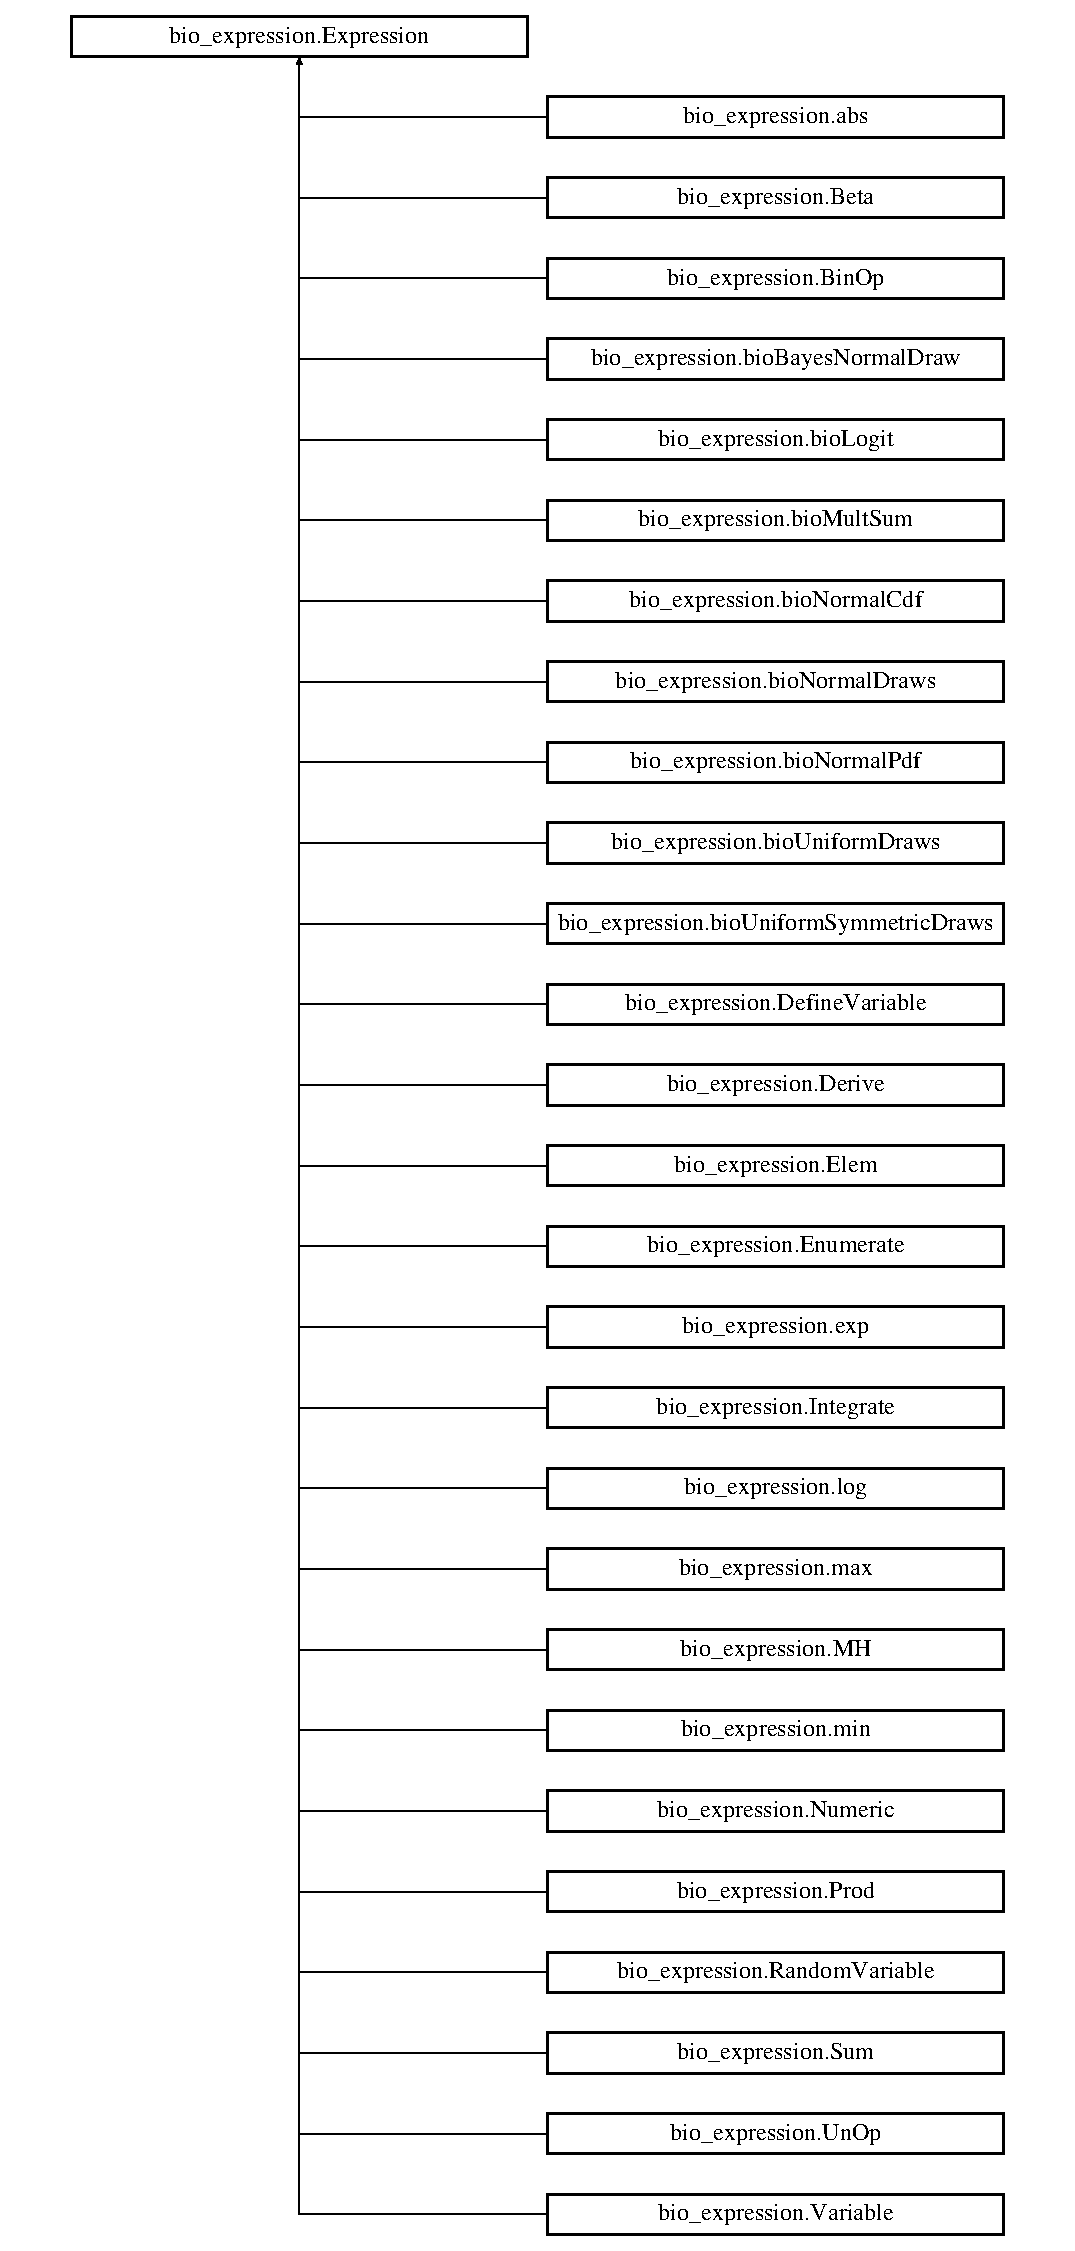
\includegraphics[height=12.000000cm]{classbio__expression_1_1_expression}
\end{center}
\end{figure}
\subsection*{Public Member Functions}
\begin{DoxyCompactItemize}
\item 
def \hyperlink{classbio__expression_1_1_expression_aa0375c4efc351d1af02688f26a41b907}{\+\_\+\+\_\+init\+\_\+\+\_\+} (self)\hypertarget{classbio__expression_1_1_expression_aa0375c4efc351d1af02688f26a41b907}{}\label{classbio__expression_1_1_expression_aa0375c4efc351d1af02688f26a41b907}

\begin{DoxyCompactList}\small\item\em Constructor. \end{DoxyCompactList}\item 
def \hyperlink{classbio__expression_1_1_expression_a38d9bf655f707d6c43b543f232c0011c}{get\+Expression} (self)
\item 
def \hyperlink{classbio__expression_1_1_expression_a4008b0b487a2b9869377be81b74c62bd}{get\+ID} (self)
\item 
def \hyperlink{classbio__expression_1_1_expression_a3de1ce140768843bb47f187c54cd5094}{\+\_\+\+\_\+str\+\_\+\+\_\+} (self)
\item 
def \hyperlink{classbio__expression_1_1_expression_a249c22deeaec778a1957939a2f38f658}{\+\_\+\+\_\+neg\+\_\+\+\_\+} (self)
\item 
def \hyperlink{classbio__expression_1_1_expression_aaa2fa7c1b65b81f4370716b4b7f13136}{\+\_\+\+\_\+add\+\_\+\+\_\+} (self, expression)
\item 
def \hyperlink{classbio__expression_1_1_expression_a9c5a8a31d20f45742f80458affa712cd}{\+\_\+\+\_\+radd\+\_\+\+\_\+} (self, expression)
\item 
def \hyperlink{classbio__expression_1_1_expression_a13dfc777e295490d603ea41dbda2aad5}{\+\_\+\+\_\+sub\+\_\+\+\_\+} (self, expression)
\item 
def \hyperlink{classbio__expression_1_1_expression_af9b2467515f7e9ab5713bbc4b5a82059}{\+\_\+\+\_\+rsub\+\_\+\+\_\+} (self, expression)
\item 
def \hyperlink{classbio__expression_1_1_expression_ac03517a41c8ba3ce8bc0b5b0e21d3753}{\+\_\+\+\_\+mul\+\_\+\+\_\+} (self, expression)
\item 
def \hyperlink{classbio__expression_1_1_expression_a33d92e31d359e040239e14260d6b389b}{\+\_\+\+\_\+rmul\+\_\+\+\_\+} (self, expression)
\item 
def \hyperlink{classbio__expression_1_1_expression_afa01bdcad97d79b90a772e7aa5e90b18}{\+\_\+\+\_\+div\+\_\+\+\_\+} (self, expression)
\item 
def \hyperlink{classbio__expression_1_1_expression_ac63454845d5703f9bc383873f46c8e91}{\+\_\+\+\_\+rdiv\+\_\+\+\_\+} (self, expression)
\item 
def \hyperlink{classbio__expression_1_1_expression_a8c1d9e629c877626bbf2d7d976c9fcd0}{\+\_\+\+\_\+truediv\+\_\+\+\_\+} (self, expression)
\begin{DoxyCompactList}\small\item\em Support for Python version 3.\+x. \end{DoxyCompactList}\item 
def \hyperlink{classbio__expression_1_1_expression_a08e1199c83badb9657f85d05792e3f76}{\+\_\+\+\_\+rtruediv\+\_\+\+\_\+} (self, expression)
\begin{DoxyCompactList}\small\item\em Support for Python version 3.\+x. \end{DoxyCompactList}\item 
def \hyperlink{classbio__expression_1_1_expression_a38c5c89581f44ccc2fb1c9b05e4dbe94}{\+\_\+\+\_\+mod\+\_\+\+\_\+} (self, expression)
\item 
def \hyperlink{classbio__expression_1_1_expression_a24fabc1dc04263664e6e0bcf79a2a473}{\+\_\+\+\_\+pow\+\_\+\+\_\+} (self, expression)
\item 
def \hyperlink{classbio__expression_1_1_expression_a46ffa545469071f702ecf5a9f1d53fc4}{\+\_\+\+\_\+rpow\+\_\+\+\_\+} (self, expression)
\item 
def \hyperlink{classbio__expression_1_1_expression_ae2059d9b654d0f6b19d97950c715c12a}{\+\_\+\+\_\+and\+\_\+\+\_\+} (self, expression)
\item 
def \hyperlink{classbio__expression_1_1_expression_a3ee80f248ac37019c6e6e971fb0a165c}{\+\_\+\+\_\+or\+\_\+\+\_\+} (self, expression)
\item 
def \hyperlink{classbio__expression_1_1_expression_a7e3e3c9535df324c51ba278044dacc6e}{\+\_\+\+\_\+eq\+\_\+\+\_\+} (self, expression)
\item 
def \hyperlink{classbio__expression_1_1_expression_a4fe08ffee3ae7d42fe2a7c41de7caa8f}{\+\_\+\+\_\+ne\+\_\+\+\_\+} (self, expression)
\item 
def \hyperlink{classbio__expression_1_1_expression_a562b739a7ba987f448138efe3d02cd1c}{\+\_\+\+\_\+le\+\_\+\+\_\+} (self, expression)
\item 
def \hyperlink{classbio__expression_1_1_expression_ad8ea5a2d766e03bb9b2bb30799d48e4f}{\+\_\+\+\_\+ge\+\_\+\+\_\+} (self, expression)
\item 
def \hyperlink{classbio__expression_1_1_expression_a04ae5af4e606bdd5717ed0b2eca1626d}{\+\_\+\+\_\+lt\+\_\+\+\_\+} (self, expression)
\item 
def \hyperlink{classbio__expression_1_1_expression_a0bb74b47fe63f9132ce35fa9c7f6104f}{\+\_\+\+\_\+gt\+\_\+\+\_\+} (self, expression)
\end{DoxyCompactItemize}
\subsection*{Public Attributes}
\begin{DoxyCompactItemize}
\item 
{\bfseries operator\+Index}\hypertarget{classbio__expression_1_1_expression_a52a16cb6e8ba6382b354164c41da65ea}{}\label{classbio__expression_1_1_expression_a52a16cb6e8ba6382b354164c41da65ea}

\end{DoxyCompactItemize}


\subsection{Detailed Description}
Interface for mathematical expressions. 

Definition at line 95 of file bio\+\_\+expression.\+py.



\subsection{Member Function Documentation}
\index{bio\+\_\+expression\+::\+Expression@{bio\+\_\+expression\+::\+Expression}!\+\_\+\+\_\+add\+\_\+\+\_\+@{\+\_\+\+\_\+add\+\_\+\+\_\+}}
\index{\+\_\+\+\_\+add\+\_\+\+\_\+@{\+\_\+\+\_\+add\+\_\+\+\_\+}!bio\+\_\+expression\+::\+Expression@{bio\+\_\+expression\+::\+Expression}}
\subsubsection[{\texorpdfstring{\+\_\+\+\_\+add\+\_\+\+\_\+(self, expression)}{__add__(self, expression)}}]{\setlength{\rightskip}{0pt plus 5cm}def bio\+\_\+expression.\+Expression.\+\_\+\+\_\+add\+\_\+\+\_\+ (
\begin{DoxyParamCaption}
\item[{}]{self, }
\item[{}]{expression}
\end{DoxyParamCaption}
)}\hypertarget{classbio__expression_1_1_expression_aaa2fa7c1b65b81f4370716b4b7f13136}{}\label{classbio__expression_1_1_expression_aaa2fa7c1b65b81f4370716b4b7f13136}

\begin{DoxyParams}{Parameters}
{\em expression} & An another expression \\
\hline
\end{DoxyParams}
\begin{DoxyReturn}{Returns}
If E is the expression, returns E + expression 
\end{DoxyReturn}


Definition at line 119 of file bio\+\_\+expression.\+py.

\index{bio\+\_\+expression\+::\+Expression@{bio\+\_\+expression\+::\+Expression}!\+\_\+\+\_\+and\+\_\+\+\_\+@{\+\_\+\+\_\+and\+\_\+\+\_\+}}
\index{\+\_\+\+\_\+and\+\_\+\+\_\+@{\+\_\+\+\_\+and\+\_\+\+\_\+}!bio\+\_\+expression\+::\+Expression@{bio\+\_\+expression\+::\+Expression}}
\subsubsection[{\texorpdfstring{\+\_\+\+\_\+and\+\_\+\+\_\+(self, expression)}{__and__(self, expression)}}]{\setlength{\rightskip}{0pt plus 5cm}def bio\+\_\+expression.\+Expression.\+\_\+\+\_\+and\+\_\+\+\_\+ (
\begin{DoxyParamCaption}
\item[{}]{self, }
\item[{}]{expression}
\end{DoxyParamCaption}
)}\hypertarget{classbio__expression_1_1_expression_ae2059d9b654d0f6b19d97950c715c12a}{}\label{classbio__expression_1_1_expression_ae2059d9b654d0f6b19d97950c715c12a}

\begin{DoxyParams}{Parameters}
{\em expression} & An another expression \\
\hline
\end{DoxyParams}
\begin{DoxyReturn}{Returns}
If E is the expression, returns E and expression 
\end{DoxyReturn}


Definition at line 186 of file bio\+\_\+expression.\+py.

\index{bio\+\_\+expression\+::\+Expression@{bio\+\_\+expression\+::\+Expression}!\+\_\+\+\_\+div\+\_\+\+\_\+@{\+\_\+\+\_\+div\+\_\+\+\_\+}}
\index{\+\_\+\+\_\+div\+\_\+\+\_\+@{\+\_\+\+\_\+div\+\_\+\+\_\+}!bio\+\_\+expression\+::\+Expression@{bio\+\_\+expression\+::\+Expression}}
\subsubsection[{\texorpdfstring{\+\_\+\+\_\+div\+\_\+\+\_\+(self, expression)}{__div__(self, expression)}}]{\setlength{\rightskip}{0pt plus 5cm}def bio\+\_\+expression.\+Expression.\+\_\+\+\_\+div\+\_\+\+\_\+ (
\begin{DoxyParamCaption}
\item[{}]{self, }
\item[{}]{expression}
\end{DoxyParamCaption}
)}\hypertarget{classbio__expression_1_1_expression_afa01bdcad97d79b90a772e7aa5e90b18}{}\label{classbio__expression_1_1_expression_afa01bdcad97d79b90a772e7aa5e90b18}

\begin{DoxyParams}{Parameters}
{\em expression} & An another expression \\
\hline
\end{DoxyParams}
\begin{DoxyReturn}{Returns}
If E is the expression, returns E / expression 
\end{DoxyReturn}


Definition at line 149 of file bio\+\_\+expression.\+py.

\index{bio\+\_\+expression\+::\+Expression@{bio\+\_\+expression\+::\+Expression}!\+\_\+\+\_\+eq\+\_\+\+\_\+@{\+\_\+\+\_\+eq\+\_\+\+\_\+}}
\index{\+\_\+\+\_\+eq\+\_\+\+\_\+@{\+\_\+\+\_\+eq\+\_\+\+\_\+}!bio\+\_\+expression\+::\+Expression@{bio\+\_\+expression\+::\+Expression}}
\subsubsection[{\texorpdfstring{\+\_\+\+\_\+eq\+\_\+\+\_\+(self, expression)}{__eq__(self, expression)}}]{\setlength{\rightskip}{0pt plus 5cm}def bio\+\_\+expression.\+Expression.\+\_\+\+\_\+eq\+\_\+\+\_\+ (
\begin{DoxyParamCaption}
\item[{}]{self, }
\item[{}]{expression}
\end{DoxyParamCaption}
)}\hypertarget{classbio__expression_1_1_expression_a7e3e3c9535df324c51ba278044dacc6e}{}\label{classbio__expression_1_1_expression_a7e3e3c9535df324c51ba278044dacc6e}

\begin{DoxyParams}{Parameters}
{\em expression} & An another expression \\
\hline
\end{DoxyParams}
\begin{DoxyReturn}{Returns}
If E is the expression, returns E == expression 
\end{DoxyReturn}


Definition at line 196 of file bio\+\_\+expression.\+py.

\index{bio\+\_\+expression\+::\+Expression@{bio\+\_\+expression\+::\+Expression}!\+\_\+\+\_\+ge\+\_\+\+\_\+@{\+\_\+\+\_\+ge\+\_\+\+\_\+}}
\index{\+\_\+\+\_\+ge\+\_\+\+\_\+@{\+\_\+\+\_\+ge\+\_\+\+\_\+}!bio\+\_\+expression\+::\+Expression@{bio\+\_\+expression\+::\+Expression}}
\subsubsection[{\texorpdfstring{\+\_\+\+\_\+ge\+\_\+\+\_\+(self, expression)}{__ge__(self, expression)}}]{\setlength{\rightskip}{0pt plus 5cm}def bio\+\_\+expression.\+Expression.\+\_\+\+\_\+ge\+\_\+\+\_\+ (
\begin{DoxyParamCaption}
\item[{}]{self, }
\item[{}]{expression}
\end{DoxyParamCaption}
)}\hypertarget{classbio__expression_1_1_expression_ad8ea5a2d766e03bb9b2bb30799d48e4f}{}\label{classbio__expression_1_1_expression_ad8ea5a2d766e03bb9b2bb30799d48e4f}

\begin{DoxyParams}{Parameters}
{\em expression} & An another expression \\
\hline
\end{DoxyParams}
\begin{DoxyReturn}{Returns}
If E is the expression, returns E $>$= expression 
\end{DoxyReturn}


Definition at line 211 of file bio\+\_\+expression.\+py.

\index{bio\+\_\+expression\+::\+Expression@{bio\+\_\+expression\+::\+Expression}!\+\_\+\+\_\+gt\+\_\+\+\_\+@{\+\_\+\+\_\+gt\+\_\+\+\_\+}}
\index{\+\_\+\+\_\+gt\+\_\+\+\_\+@{\+\_\+\+\_\+gt\+\_\+\+\_\+}!bio\+\_\+expression\+::\+Expression@{bio\+\_\+expression\+::\+Expression}}
\subsubsection[{\texorpdfstring{\+\_\+\+\_\+gt\+\_\+\+\_\+(self, expression)}{__gt__(self, expression)}}]{\setlength{\rightskip}{0pt plus 5cm}def bio\+\_\+expression.\+Expression.\+\_\+\+\_\+gt\+\_\+\+\_\+ (
\begin{DoxyParamCaption}
\item[{}]{self, }
\item[{}]{expression}
\end{DoxyParamCaption}
)}\hypertarget{classbio__expression_1_1_expression_a0bb74b47fe63f9132ce35fa9c7f6104f}{}\label{classbio__expression_1_1_expression_a0bb74b47fe63f9132ce35fa9c7f6104f}

\begin{DoxyParams}{Parameters}
{\em expression} & An another expression \\
\hline
\end{DoxyParams}
\begin{DoxyReturn}{Returns}
If E is the expression, returns E $>$ expression 
\end{DoxyReturn}


Definition at line 221 of file bio\+\_\+expression.\+py.

\index{bio\+\_\+expression\+::\+Expression@{bio\+\_\+expression\+::\+Expression}!\+\_\+\+\_\+le\+\_\+\+\_\+@{\+\_\+\+\_\+le\+\_\+\+\_\+}}
\index{\+\_\+\+\_\+le\+\_\+\+\_\+@{\+\_\+\+\_\+le\+\_\+\+\_\+}!bio\+\_\+expression\+::\+Expression@{bio\+\_\+expression\+::\+Expression}}
\subsubsection[{\texorpdfstring{\+\_\+\+\_\+le\+\_\+\+\_\+(self, expression)}{__le__(self, expression)}}]{\setlength{\rightskip}{0pt plus 5cm}def bio\+\_\+expression.\+Expression.\+\_\+\+\_\+le\+\_\+\+\_\+ (
\begin{DoxyParamCaption}
\item[{}]{self, }
\item[{}]{expression}
\end{DoxyParamCaption}
)}\hypertarget{classbio__expression_1_1_expression_a562b739a7ba987f448138efe3d02cd1c}{}\label{classbio__expression_1_1_expression_a562b739a7ba987f448138efe3d02cd1c}

\begin{DoxyParams}{Parameters}
{\em expression} & An another expression \\
\hline
\end{DoxyParams}
\begin{DoxyReturn}{Returns}
If E is the expression, returns E $<$= expression 
\end{DoxyReturn}


Definition at line 206 of file bio\+\_\+expression.\+py.

\index{bio\+\_\+expression\+::\+Expression@{bio\+\_\+expression\+::\+Expression}!\+\_\+\+\_\+lt\+\_\+\+\_\+@{\+\_\+\+\_\+lt\+\_\+\+\_\+}}
\index{\+\_\+\+\_\+lt\+\_\+\+\_\+@{\+\_\+\+\_\+lt\+\_\+\+\_\+}!bio\+\_\+expression\+::\+Expression@{bio\+\_\+expression\+::\+Expression}}
\subsubsection[{\texorpdfstring{\+\_\+\+\_\+lt\+\_\+\+\_\+(self, expression)}{__lt__(self, expression)}}]{\setlength{\rightskip}{0pt plus 5cm}def bio\+\_\+expression.\+Expression.\+\_\+\+\_\+lt\+\_\+\+\_\+ (
\begin{DoxyParamCaption}
\item[{}]{self, }
\item[{}]{expression}
\end{DoxyParamCaption}
)}\hypertarget{classbio__expression_1_1_expression_a04ae5af4e606bdd5717ed0b2eca1626d}{}\label{classbio__expression_1_1_expression_a04ae5af4e606bdd5717ed0b2eca1626d}

\begin{DoxyParams}{Parameters}
{\em expression} & An another expression \\
\hline
\end{DoxyParams}
\begin{DoxyReturn}{Returns}
If E is the expression, returns E $<$ expression 
\end{DoxyReturn}


Definition at line 216 of file bio\+\_\+expression.\+py.

\index{bio\+\_\+expression\+::\+Expression@{bio\+\_\+expression\+::\+Expression}!\+\_\+\+\_\+mod\+\_\+\+\_\+@{\+\_\+\+\_\+mod\+\_\+\+\_\+}}
\index{\+\_\+\+\_\+mod\+\_\+\+\_\+@{\+\_\+\+\_\+mod\+\_\+\+\_\+}!bio\+\_\+expression\+::\+Expression@{bio\+\_\+expression\+::\+Expression}}
\subsubsection[{\texorpdfstring{\+\_\+\+\_\+mod\+\_\+\+\_\+(self, expression)}{__mod__(self, expression)}}]{\setlength{\rightskip}{0pt plus 5cm}def bio\+\_\+expression.\+Expression.\+\_\+\+\_\+mod\+\_\+\+\_\+ (
\begin{DoxyParamCaption}
\item[{}]{self, }
\item[{}]{expression}
\end{DoxyParamCaption}
)}\hypertarget{classbio__expression_1_1_expression_a38c5c89581f44ccc2fb1c9b05e4dbe94}{}\label{classbio__expression_1_1_expression_a38c5c89581f44ccc2fb1c9b05e4dbe94}

\begin{DoxyParams}{Parameters}
{\em expression} & An another expression \\
\hline
\end{DoxyParams}
\begin{DoxyReturn}{Returns}
If E is the expression, returns E \% expression (modulo) 
\end{DoxyReturn}


Definition at line 171 of file bio\+\_\+expression.\+py.

\index{bio\+\_\+expression\+::\+Expression@{bio\+\_\+expression\+::\+Expression}!\+\_\+\+\_\+mul\+\_\+\+\_\+@{\+\_\+\+\_\+mul\+\_\+\+\_\+}}
\index{\+\_\+\+\_\+mul\+\_\+\+\_\+@{\+\_\+\+\_\+mul\+\_\+\+\_\+}!bio\+\_\+expression\+::\+Expression@{bio\+\_\+expression\+::\+Expression}}
\subsubsection[{\texorpdfstring{\+\_\+\+\_\+mul\+\_\+\+\_\+(self, expression)}{__mul__(self, expression)}}]{\setlength{\rightskip}{0pt plus 5cm}def bio\+\_\+expression.\+Expression.\+\_\+\+\_\+mul\+\_\+\+\_\+ (
\begin{DoxyParamCaption}
\item[{}]{self, }
\item[{}]{expression}
\end{DoxyParamCaption}
)}\hypertarget{classbio__expression_1_1_expression_ac03517a41c8ba3ce8bc0b5b0e21d3753}{}\label{classbio__expression_1_1_expression_ac03517a41c8ba3ce8bc0b5b0e21d3753}

\begin{DoxyParams}{Parameters}
{\em expression} & An another expression \\
\hline
\end{DoxyParams}
\begin{DoxyReturn}{Returns}
If E is the expression, returns E $\ast$ expression 
\end{DoxyReturn}


Definition at line 139 of file bio\+\_\+expression.\+py.

\index{bio\+\_\+expression\+::\+Expression@{bio\+\_\+expression\+::\+Expression}!\+\_\+\+\_\+ne\+\_\+\+\_\+@{\+\_\+\+\_\+ne\+\_\+\+\_\+}}
\index{\+\_\+\+\_\+ne\+\_\+\+\_\+@{\+\_\+\+\_\+ne\+\_\+\+\_\+}!bio\+\_\+expression\+::\+Expression@{bio\+\_\+expression\+::\+Expression}}
\subsubsection[{\texorpdfstring{\+\_\+\+\_\+ne\+\_\+\+\_\+(self, expression)}{__ne__(self, expression)}}]{\setlength{\rightskip}{0pt plus 5cm}def bio\+\_\+expression.\+Expression.\+\_\+\+\_\+ne\+\_\+\+\_\+ (
\begin{DoxyParamCaption}
\item[{}]{self, }
\item[{}]{expression}
\end{DoxyParamCaption}
)}\hypertarget{classbio__expression_1_1_expression_a4fe08ffee3ae7d42fe2a7c41de7caa8f}{}\label{classbio__expression_1_1_expression_a4fe08ffee3ae7d42fe2a7c41de7caa8f}

\begin{DoxyParams}{Parameters}
{\em expression} & An another expression \\
\hline
\end{DoxyParams}
\begin{DoxyReturn}{Returns}
If E is the expression, returns E != expression 
\end{DoxyReturn}


Definition at line 201 of file bio\+\_\+expression.\+py.

\index{bio\+\_\+expression\+::\+Expression@{bio\+\_\+expression\+::\+Expression}!\+\_\+\+\_\+neg\+\_\+\+\_\+@{\+\_\+\+\_\+neg\+\_\+\+\_\+}}
\index{\+\_\+\+\_\+neg\+\_\+\+\_\+@{\+\_\+\+\_\+neg\+\_\+\+\_\+}!bio\+\_\+expression\+::\+Expression@{bio\+\_\+expression\+::\+Expression}}
\subsubsection[{\texorpdfstring{\+\_\+\+\_\+neg\+\_\+\+\_\+(self)}{__neg__(self)}}]{\setlength{\rightskip}{0pt plus 5cm}def bio\+\_\+expression.\+Expression.\+\_\+\+\_\+neg\+\_\+\+\_\+ (
\begin{DoxyParamCaption}
\item[{}]{self}
\end{DoxyParamCaption}
)}\hypertarget{classbio__expression_1_1_expression_a249c22deeaec778a1957939a2f38f658}{}\label{classbio__expression_1_1_expression_a249c22deeaec778a1957939a2f38f658}
\begin{DoxyReturn}{Returns}
If E is the expression, returns -\/E 
\end{DoxyReturn}


Definition at line 114 of file bio\+\_\+expression.\+py.

\index{bio\+\_\+expression\+::\+Expression@{bio\+\_\+expression\+::\+Expression}!\+\_\+\+\_\+or\+\_\+\+\_\+@{\+\_\+\+\_\+or\+\_\+\+\_\+}}
\index{\+\_\+\+\_\+or\+\_\+\+\_\+@{\+\_\+\+\_\+or\+\_\+\+\_\+}!bio\+\_\+expression\+::\+Expression@{bio\+\_\+expression\+::\+Expression}}
\subsubsection[{\texorpdfstring{\+\_\+\+\_\+or\+\_\+\+\_\+(self, expression)}{__or__(self, expression)}}]{\setlength{\rightskip}{0pt plus 5cm}def bio\+\_\+expression.\+Expression.\+\_\+\+\_\+or\+\_\+\+\_\+ (
\begin{DoxyParamCaption}
\item[{}]{self, }
\item[{}]{expression}
\end{DoxyParamCaption}
)}\hypertarget{classbio__expression_1_1_expression_a3ee80f248ac37019c6e6e971fb0a165c}{}\label{classbio__expression_1_1_expression_a3ee80f248ac37019c6e6e971fb0a165c}

\begin{DoxyParams}{Parameters}
{\em expression} & An another expression \\
\hline
\end{DoxyParams}
\begin{DoxyReturn}{Returns}
If E is the expression, returns E or expression 
\end{DoxyReturn}


Definition at line 191 of file bio\+\_\+expression.\+py.

\index{bio\+\_\+expression\+::\+Expression@{bio\+\_\+expression\+::\+Expression}!\+\_\+\+\_\+pow\+\_\+\+\_\+@{\+\_\+\+\_\+pow\+\_\+\+\_\+}}
\index{\+\_\+\+\_\+pow\+\_\+\+\_\+@{\+\_\+\+\_\+pow\+\_\+\+\_\+}!bio\+\_\+expression\+::\+Expression@{bio\+\_\+expression\+::\+Expression}}
\subsubsection[{\texorpdfstring{\+\_\+\+\_\+pow\+\_\+\+\_\+(self, expression)}{__pow__(self, expression)}}]{\setlength{\rightskip}{0pt plus 5cm}def bio\+\_\+expression.\+Expression.\+\_\+\+\_\+pow\+\_\+\+\_\+ (
\begin{DoxyParamCaption}
\item[{}]{self, }
\item[{}]{expression}
\end{DoxyParamCaption}
)}\hypertarget{classbio__expression_1_1_expression_a24fabc1dc04263664e6e0bcf79a2a473}{}\label{classbio__expression_1_1_expression_a24fabc1dc04263664e6e0bcf79a2a473}

\begin{DoxyParams}{Parameters}
{\em expression} & An another expression \\
\hline
\end{DoxyParams}
\begin{DoxyReturn}{Returns}
If E is the expression, returns E $^\wedge$ expression 
\end{DoxyReturn}


Definition at line 176 of file bio\+\_\+expression.\+py.

\index{bio\+\_\+expression\+::\+Expression@{bio\+\_\+expression\+::\+Expression}!\+\_\+\+\_\+radd\+\_\+\+\_\+@{\+\_\+\+\_\+radd\+\_\+\+\_\+}}
\index{\+\_\+\+\_\+radd\+\_\+\+\_\+@{\+\_\+\+\_\+radd\+\_\+\+\_\+}!bio\+\_\+expression\+::\+Expression@{bio\+\_\+expression\+::\+Expression}}
\subsubsection[{\texorpdfstring{\+\_\+\+\_\+radd\+\_\+\+\_\+(self, expression)}{__radd__(self, expression)}}]{\setlength{\rightskip}{0pt plus 5cm}def bio\+\_\+expression.\+Expression.\+\_\+\+\_\+radd\+\_\+\+\_\+ (
\begin{DoxyParamCaption}
\item[{}]{self, }
\item[{}]{expression}
\end{DoxyParamCaption}
)}\hypertarget{classbio__expression_1_1_expression_a9c5a8a31d20f45742f80458affa712cd}{}\label{classbio__expression_1_1_expression_a9c5a8a31d20f45742f80458affa712cd}

\begin{DoxyParams}{Parameters}
{\em expression} & An another expression \\
\hline
\end{DoxyParams}
\begin{DoxyReturn}{Returns}
If E is the expression, returns expression + E 
\end{DoxyReturn}


Definition at line 124 of file bio\+\_\+expression.\+py.

\index{bio\+\_\+expression\+::\+Expression@{bio\+\_\+expression\+::\+Expression}!\+\_\+\+\_\+rdiv\+\_\+\+\_\+@{\+\_\+\+\_\+rdiv\+\_\+\+\_\+}}
\index{\+\_\+\+\_\+rdiv\+\_\+\+\_\+@{\+\_\+\+\_\+rdiv\+\_\+\+\_\+}!bio\+\_\+expression\+::\+Expression@{bio\+\_\+expression\+::\+Expression}}
\subsubsection[{\texorpdfstring{\+\_\+\+\_\+rdiv\+\_\+\+\_\+(self, expression)}{__rdiv__(self, expression)}}]{\setlength{\rightskip}{0pt plus 5cm}def bio\+\_\+expression.\+Expression.\+\_\+\+\_\+rdiv\+\_\+\+\_\+ (
\begin{DoxyParamCaption}
\item[{}]{self, }
\item[{}]{expression}
\end{DoxyParamCaption}
)}\hypertarget{classbio__expression_1_1_expression_ac63454845d5703f9bc383873f46c8e91}{}\label{classbio__expression_1_1_expression_ac63454845d5703f9bc383873f46c8e91}

\begin{DoxyParams}{Parameters}
{\em expression} & An another expression \\
\hline
\end{DoxyParams}
\begin{DoxyReturn}{Returns}
If E is the expression, returns expression / E 
\end{DoxyReturn}


Definition at line 154 of file bio\+\_\+expression.\+py.

\index{bio\+\_\+expression\+::\+Expression@{bio\+\_\+expression\+::\+Expression}!\+\_\+\+\_\+rmul\+\_\+\+\_\+@{\+\_\+\+\_\+rmul\+\_\+\+\_\+}}
\index{\+\_\+\+\_\+rmul\+\_\+\+\_\+@{\+\_\+\+\_\+rmul\+\_\+\+\_\+}!bio\+\_\+expression\+::\+Expression@{bio\+\_\+expression\+::\+Expression}}
\subsubsection[{\texorpdfstring{\+\_\+\+\_\+rmul\+\_\+\+\_\+(self, expression)}{__rmul__(self, expression)}}]{\setlength{\rightskip}{0pt plus 5cm}def bio\+\_\+expression.\+Expression.\+\_\+\+\_\+rmul\+\_\+\+\_\+ (
\begin{DoxyParamCaption}
\item[{}]{self, }
\item[{}]{expression}
\end{DoxyParamCaption}
)}\hypertarget{classbio__expression_1_1_expression_a33d92e31d359e040239e14260d6b389b}{}\label{classbio__expression_1_1_expression_a33d92e31d359e040239e14260d6b389b}

\begin{DoxyParams}{Parameters}
{\em expression} & An another expression \\
\hline
\end{DoxyParams}
\begin{DoxyReturn}{Returns}
If E is the expression, returns expression $\ast$ E 
\end{DoxyReturn}


Definition at line 144 of file bio\+\_\+expression.\+py.

\index{bio\+\_\+expression\+::\+Expression@{bio\+\_\+expression\+::\+Expression}!\+\_\+\+\_\+rpow\+\_\+\+\_\+@{\+\_\+\+\_\+rpow\+\_\+\+\_\+}}
\index{\+\_\+\+\_\+rpow\+\_\+\+\_\+@{\+\_\+\+\_\+rpow\+\_\+\+\_\+}!bio\+\_\+expression\+::\+Expression@{bio\+\_\+expression\+::\+Expression}}
\subsubsection[{\texorpdfstring{\+\_\+\+\_\+rpow\+\_\+\+\_\+(self, expression)}{__rpow__(self, expression)}}]{\setlength{\rightskip}{0pt plus 5cm}def bio\+\_\+expression.\+Expression.\+\_\+\+\_\+rpow\+\_\+\+\_\+ (
\begin{DoxyParamCaption}
\item[{}]{self, }
\item[{}]{expression}
\end{DoxyParamCaption}
)}\hypertarget{classbio__expression_1_1_expression_a46ffa545469071f702ecf5a9f1d53fc4}{}\label{classbio__expression_1_1_expression_a46ffa545469071f702ecf5a9f1d53fc4}

\begin{DoxyParams}{Parameters}
{\em expression} & An another expression \\
\hline
\end{DoxyParams}
\begin{DoxyReturn}{Returns}
If E is the expression, returns expression $^\wedge$ E 
\end{DoxyReturn}


Definition at line 181 of file bio\+\_\+expression.\+py.

\index{bio\+\_\+expression\+::\+Expression@{bio\+\_\+expression\+::\+Expression}!\+\_\+\+\_\+rsub\+\_\+\+\_\+@{\+\_\+\+\_\+rsub\+\_\+\+\_\+}}
\index{\+\_\+\+\_\+rsub\+\_\+\+\_\+@{\+\_\+\+\_\+rsub\+\_\+\+\_\+}!bio\+\_\+expression\+::\+Expression@{bio\+\_\+expression\+::\+Expression}}
\subsubsection[{\texorpdfstring{\+\_\+\+\_\+rsub\+\_\+\+\_\+(self, expression)}{__rsub__(self, expression)}}]{\setlength{\rightskip}{0pt plus 5cm}def bio\+\_\+expression.\+Expression.\+\_\+\+\_\+rsub\+\_\+\+\_\+ (
\begin{DoxyParamCaption}
\item[{}]{self, }
\item[{}]{expression}
\end{DoxyParamCaption}
)}\hypertarget{classbio__expression_1_1_expression_af9b2467515f7e9ab5713bbc4b5a82059}{}\label{classbio__expression_1_1_expression_af9b2467515f7e9ab5713bbc4b5a82059}

\begin{DoxyParams}{Parameters}
{\em expression} & An another expression \\
\hline
\end{DoxyParams}
\begin{DoxyReturn}{Returns}
If E is the expression, returns expression -\/ E 
\end{DoxyReturn}


Definition at line 134 of file bio\+\_\+expression.\+py.

\index{bio\+\_\+expression\+::\+Expression@{bio\+\_\+expression\+::\+Expression}!\+\_\+\+\_\+rtruediv\+\_\+\+\_\+@{\+\_\+\+\_\+rtruediv\+\_\+\+\_\+}}
\index{\+\_\+\+\_\+rtruediv\+\_\+\+\_\+@{\+\_\+\+\_\+rtruediv\+\_\+\+\_\+}!bio\+\_\+expression\+::\+Expression@{bio\+\_\+expression\+::\+Expression}}
\subsubsection[{\texorpdfstring{\+\_\+\+\_\+rtruediv\+\_\+\+\_\+(self, expression)}{__rtruediv__(self, expression)}}]{\setlength{\rightskip}{0pt plus 5cm}def bio\+\_\+expression.\+Expression.\+\_\+\+\_\+rtruediv\+\_\+\+\_\+ (
\begin{DoxyParamCaption}
\item[{}]{self, }
\item[{}]{expression}
\end{DoxyParamCaption}
)}\hypertarget{classbio__expression_1_1_expression_a08e1199c83badb9657f85d05792e3f76}{}\label{classbio__expression_1_1_expression_a08e1199c83badb9657f85d05792e3f76}


Support for Python version 3.\+x. 


\begin{DoxyParams}{Parameters}
{\em expression} & An another expression \\
\hline
\end{DoxyParams}
\begin{DoxyReturn}{Returns}
If E is the expression, returns expression / E 
\end{DoxyReturn}


Definition at line 166 of file bio\+\_\+expression.\+py.

\index{bio\+\_\+expression\+::\+Expression@{bio\+\_\+expression\+::\+Expression}!\+\_\+\+\_\+str\+\_\+\+\_\+@{\+\_\+\+\_\+str\+\_\+\+\_\+}}
\index{\+\_\+\+\_\+str\+\_\+\+\_\+@{\+\_\+\+\_\+str\+\_\+\+\_\+}!bio\+\_\+expression\+::\+Expression@{bio\+\_\+expression\+::\+Expression}}
\subsubsection[{\texorpdfstring{\+\_\+\+\_\+str\+\_\+\+\_\+(self)}{__str__(self)}}]{\setlength{\rightskip}{0pt plus 5cm}def bio\+\_\+expression.\+Expression.\+\_\+\+\_\+str\+\_\+\+\_\+ (
\begin{DoxyParamCaption}
\item[{}]{self}
\end{DoxyParamCaption}
)}\hypertarget{classbio__expression_1_1_expression_a3de1ce140768843bb47f187c54cd5094}{}\label{classbio__expression_1_1_expression_a3de1ce140768843bb47f187c54cd5094}
\begin{DoxyReturn}{Returns}
Returns a string with the expression 
\end{DoxyReturn}


Definition at line 110 of file bio\+\_\+expression.\+py.

\index{bio\+\_\+expression\+::\+Expression@{bio\+\_\+expression\+::\+Expression}!\+\_\+\+\_\+sub\+\_\+\+\_\+@{\+\_\+\+\_\+sub\+\_\+\+\_\+}}
\index{\+\_\+\+\_\+sub\+\_\+\+\_\+@{\+\_\+\+\_\+sub\+\_\+\+\_\+}!bio\+\_\+expression\+::\+Expression@{bio\+\_\+expression\+::\+Expression}}
\subsubsection[{\texorpdfstring{\+\_\+\+\_\+sub\+\_\+\+\_\+(self, expression)}{__sub__(self, expression)}}]{\setlength{\rightskip}{0pt plus 5cm}def bio\+\_\+expression.\+Expression.\+\_\+\+\_\+sub\+\_\+\+\_\+ (
\begin{DoxyParamCaption}
\item[{}]{self, }
\item[{}]{expression}
\end{DoxyParamCaption}
)}\hypertarget{classbio__expression_1_1_expression_a13dfc777e295490d603ea41dbda2aad5}{}\label{classbio__expression_1_1_expression_a13dfc777e295490d603ea41dbda2aad5}

\begin{DoxyParams}{Parameters}
{\em expression} & An another expression \\
\hline
\end{DoxyParams}
\begin{DoxyReturn}{Returns}
If E is the expression, returns E -\/ expression 
\end{DoxyReturn}


Definition at line 129 of file bio\+\_\+expression.\+py.

\index{bio\+\_\+expression\+::\+Expression@{bio\+\_\+expression\+::\+Expression}!\+\_\+\+\_\+truediv\+\_\+\+\_\+@{\+\_\+\+\_\+truediv\+\_\+\+\_\+}}
\index{\+\_\+\+\_\+truediv\+\_\+\+\_\+@{\+\_\+\+\_\+truediv\+\_\+\+\_\+}!bio\+\_\+expression\+::\+Expression@{bio\+\_\+expression\+::\+Expression}}
\subsubsection[{\texorpdfstring{\+\_\+\+\_\+truediv\+\_\+\+\_\+(self, expression)}{__truediv__(self, expression)}}]{\setlength{\rightskip}{0pt plus 5cm}def bio\+\_\+expression.\+Expression.\+\_\+\+\_\+truediv\+\_\+\+\_\+ (
\begin{DoxyParamCaption}
\item[{}]{self, }
\item[{}]{expression}
\end{DoxyParamCaption}
)}\hypertarget{classbio__expression_1_1_expression_a8c1d9e629c877626bbf2d7d976c9fcd0}{}\label{classbio__expression_1_1_expression_a8c1d9e629c877626bbf2d7d976c9fcd0}


Support for Python version 3.\+x. 


\begin{DoxyParams}{Parameters}
{\em expression} & An another expression \\
\hline
\end{DoxyParams}
\begin{DoxyReturn}{Returns}
If E is the expression, returns E / expression 
\end{DoxyReturn}


Definition at line 160 of file bio\+\_\+expression.\+py.

\index{bio\+\_\+expression\+::\+Expression@{bio\+\_\+expression\+::\+Expression}!get\+Expression@{get\+Expression}}
\index{get\+Expression@{get\+Expression}!bio\+\_\+expression\+::\+Expression@{bio\+\_\+expression\+::\+Expression}}
\subsubsection[{\texorpdfstring{get\+Expression(self)}{getExpression(self)}}]{\setlength{\rightskip}{0pt plus 5cm}def bio\+\_\+expression.\+Expression.\+get\+Expression (
\begin{DoxyParamCaption}
\item[{}]{self}
\end{DoxyParamCaption}
)}\hypertarget{classbio__expression_1_1_expression_a38d9bf655f707d6c43b543f232c0011c}{}\label{classbio__expression_1_1_expression_a38d9bf655f707d6c43b543f232c0011c}
\begin{DoxyReturn}{Returns}
Return the string representation of the current expression 
\end{DoxyReturn}


Definition at line 102 of file bio\+\_\+expression.\+py.

\index{bio\+\_\+expression\+::\+Expression@{bio\+\_\+expression\+::\+Expression}!get\+ID@{get\+ID}}
\index{get\+ID@{get\+ID}!bio\+\_\+expression\+::\+Expression@{bio\+\_\+expression\+::\+Expression}}
\subsubsection[{\texorpdfstring{get\+I\+D(self)}{getID(self)}}]{\setlength{\rightskip}{0pt plus 5cm}def bio\+\_\+expression.\+Expression.\+get\+ID (
\begin{DoxyParamCaption}
\item[{}]{self}
\end{DoxyParamCaption}
)}\hypertarget{classbio__expression_1_1_expression_a4008b0b487a2b9869377be81b74c62bd}{}\label{classbio__expression_1_1_expression_a4008b0b487a2b9869377be81b74c62bd}
\begin{DoxyReturn}{Returns}
Return an ID for this expression, can be \char`\"{}xx-\/no I\+D\char`\"{} if the sublcass doest not override the function 
\end{DoxyReturn}


Definition at line 106 of file bio\+\_\+expression.\+py.



The documentation for this class was generated from the following file\+:\begin{DoxyCompactItemize}
\item 
\hyperlink{bio__expression_8py}{bio\+\_\+expression.\+py}\end{DoxyCompactItemize}

\hypertarget{classbio__expression_1_1_integrate}{\section{bio\+\_\+expression.\+Integrate Class Reference}
\label{classbio__expression_1_1_integrate}\index{bio\+\_\+expression.\+Integrate@{bio\+\_\+expression.\+Integrate}}
}


Class performing numerical integration relying on the \href{http://en.wikipedia.org/wiki/Gaussian_quadrature}{\tt Gauss-\/\+Hermite quadrature} to compute \[ \int_{-\infty}^{+\infty} f(\omega) d\omega. \].  


Inheritance diagram for bio\+\_\+expression.\+Integrate\+:\begin{figure}[H]
\begin{center}
\leavevmode
\includegraphics[height=2.000000cm]{d2/dd1/classbio__expression_1_1_integrate}
\end{center}
\end{figure}
\subsection*{Public Member Functions}
\begin{DoxyCompactItemize}
\item 
def \hyperlink{classbio__expression_1_1_integrate_a0ce66b3a16e295afdb7c6f0819f46d6d}{\+\_\+\+\_\+init\+\_\+\+\_\+}
\item 
def \hyperlink{classbio__expression_1_1_integrate_a1aff67b31caf78c898f342ccc4c52a80}{get\+Expression}
\end{DoxyCompactItemize}
\subsection*{Public Attributes}
\begin{DoxyCompactItemize}
\item 
\hyperlink{classbio__expression_1_1_integrate_aa0b26e5e7ef188bddbbbac6d2734eb1e}{function}
\item 
\hyperlink{classbio__expression_1_1_integrate_a8aa2ae870cce644d72a76ecae5497121}{variable}
\item 
\hyperlink{classbio__expression_1_1_integrate_ae6f4e73d2daf792fc223e12b205c4904}{operator\+Index}
\end{DoxyCompactItemize}


\subsection{Detailed Description}
Class performing numerical integration relying on the \href{http://en.wikipedia.org/wiki/Gaussian_quadrature}{\tt Gauss-\/\+Hermite quadrature} to compute \[ \int_{-\infty}^{+\infty} f(\omega) d\omega. \]. 

As an example, the computation of a normal mixture of logit models is performed using the following syntax, where condprob is the conditional (logit) choice probability\+: 
\begin{DoxyCode}
1 omega = RandomVariable(\textcolor{stringliteral}{'omega'})
2 density = bioNormalPdf(omega) 
3 result = Integrate(condprob * density,\textcolor{stringliteral}{'omega'})
\end{DoxyCode}
 Comments\+:
\begin{DoxyItemize}
\item The Gauss-\/\+Hermite procedure is designed to compute integrals of the form \[ \int_{-\infty}^{+\infty} e^{-\omega^2} f(\omega) d\omega. \] Therefore, Biogeme multiplies the expression by $e^{\omega^2}$ before applying the Gauss-\/\+Hermite algorithm. This is transparent for the user.
\end{DoxyItemize}

It is usually more accurate to compute an integral using a quadrature procedure. However, it should be used only in the presence of few (one or two) random variables. The same integral can be computed using Monte-\/\+Carlo integration using the following syntax\+: 
\begin{DoxyCode}
1 omega = bioNormalDraws(\textcolor{stringliteral}{'omega'})
2 drawIterator(\textcolor{stringliteral}{'drawIter'})
3 result = Sum(condprob,\textcolor{stringliteral}{'drawIter'})
\end{DoxyCode}
 

\subsection{Constructor \& Destructor Documentation}
\hypertarget{classbio__expression_1_1_integrate_a0ce66b3a16e295afdb7c6f0819f46d6d}{\index{bio\+\_\+expression\+::\+Integrate@{bio\+\_\+expression\+::\+Integrate}!\+\_\+\+\_\+init\+\_\+\+\_\+@{\+\_\+\+\_\+init\+\_\+\+\_\+}}
\index{\+\_\+\+\_\+init\+\_\+\+\_\+@{\+\_\+\+\_\+init\+\_\+\+\_\+}!bio\+\_\+expression\+::\+Integrate@{bio\+\_\+expression\+::\+Integrate}}
\subsubsection[{\+\_\+\+\_\+init\+\_\+\+\_\+}]{\setlength{\rightskip}{0pt plus 5cm}def bio\+\_\+expression.\+Integrate.\+\_\+\+\_\+init\+\_\+\+\_\+ (
\begin{DoxyParamCaption}
\item[{}]{self, }
\item[{}]{term, }
\item[{}]{v}
\end{DoxyParamCaption}
)}}\label{classbio__expression_1_1_integrate_a0ce66b3a16e295afdb7c6f0819f46d6d}

\begin{DoxyParams}{Parameters}
{\em term} & any valid \hyperlink{namespacebio__expression}{bio\+\_\+expression} representing the expression to integrate \\
\hline
{\em v} & name of the integration variable, previously defined using a bio\+Expression\+::\+Random\+Variable statement. \\
\hline
\end{DoxyParams}


\subsection{Member Function Documentation}
\hypertarget{classbio__expression_1_1_integrate_a1aff67b31caf78c898f342ccc4c52a80}{\index{bio\+\_\+expression\+::\+Integrate@{bio\+\_\+expression\+::\+Integrate}!get\+Expression@{get\+Expression}}
\index{get\+Expression@{get\+Expression}!bio\+\_\+expression\+::\+Integrate@{bio\+\_\+expression\+::\+Integrate}}
\subsubsection[{get\+Expression}]{\setlength{\rightskip}{0pt plus 5cm}def bio\+\_\+expression.\+Integrate.\+get\+Expression (
\begin{DoxyParamCaption}
\item[{}]{self}
\end{DoxyParamCaption}
)}}\label{classbio__expression_1_1_integrate_a1aff67b31caf78c898f342ccc4c52a80}


\subsection{Member Data Documentation}
\hypertarget{classbio__expression_1_1_integrate_aa0b26e5e7ef188bddbbbac6d2734eb1e}{\index{bio\+\_\+expression\+::\+Integrate@{bio\+\_\+expression\+::\+Integrate}!function@{function}}
\index{function@{function}!bio\+\_\+expression\+::\+Integrate@{bio\+\_\+expression\+::\+Integrate}}
\subsubsection[{function}]{\setlength{\rightskip}{0pt plus 5cm}bio\+\_\+expression.\+Integrate.\+function}}\label{classbio__expression_1_1_integrate_aa0b26e5e7ef188bddbbbac6d2734eb1e}
\hypertarget{classbio__expression_1_1_integrate_ae6f4e73d2daf792fc223e12b205c4904}{\index{bio\+\_\+expression\+::\+Integrate@{bio\+\_\+expression\+::\+Integrate}!operator\+Index@{operator\+Index}}
\index{operator\+Index@{operator\+Index}!bio\+\_\+expression\+::\+Integrate@{bio\+\_\+expression\+::\+Integrate}}
\subsubsection[{operator\+Index}]{\setlength{\rightskip}{0pt plus 5cm}bio\+\_\+expression.\+Integrate.\+operator\+Index}}\label{classbio__expression_1_1_integrate_ae6f4e73d2daf792fc223e12b205c4904}
\hypertarget{classbio__expression_1_1_integrate_a8aa2ae870cce644d72a76ecae5497121}{\index{bio\+\_\+expression\+::\+Integrate@{bio\+\_\+expression\+::\+Integrate}!variable@{variable}}
\index{variable@{variable}!bio\+\_\+expression\+::\+Integrate@{bio\+\_\+expression\+::\+Integrate}}
\subsubsection[{variable}]{\setlength{\rightskip}{0pt plus 5cm}bio\+\_\+expression.\+Integrate.\+variable}}\label{classbio__expression_1_1_integrate_a8aa2ae870cce644d72a76ecae5497121}


The documentation for this class was generated from the following file\+:\begin{DoxyCompactItemize}
\item 
\hyperlink{bio__expression_8py}{bio\+\_\+expression.\+py}\end{DoxyCompactItemize}

\hypertarget{classbio__iterator_1_1iterator}{}\section{bio\+\_\+iterator.\+iterator Class Reference}
\label{classbio__iterator_1_1iterator}\index{bio\+\_\+iterator.\+iterator@{bio\+\_\+iterator.\+iterator}}


Generic class for an iterator.  


Inheritance diagram for bio\+\_\+iterator.\+iterator\+:\begin{figure}[H]
\begin{center}
\leavevmode
\includegraphics[height=2.000000cm]{classbio__iterator_1_1iterator}
\end{center}
\end{figure}
\subsection*{Public Member Functions}
\begin{DoxyCompactItemize}
\item 
def {\bfseries \+\_\+\+\_\+init\+\_\+\+\_\+} (self, iterator\+Name, name, child, variable)\hypertarget{classbio__iterator_1_1iterator_a938eec8f7f8398efabc0e94e0e69a9c7}{}\label{classbio__iterator_1_1iterator_a938eec8f7f8398efabc0e94e0e69a9c7}

\item 
def {\bfseries \+\_\+\+\_\+str\+\_\+\+\_\+} (self)\hypertarget{classbio__iterator_1_1iterator_a3015cba9030f10b6de833c03f632fa2a}{}\label{classbio__iterator_1_1iterator_a3015cba9030f10b6de833c03f632fa2a}

\end{DoxyCompactItemize}
\subsection*{Public Attributes}
\begin{DoxyCompactItemize}
\item 
{\bfseries iterator\+Name}\hypertarget{classbio__iterator_1_1iterator_a10e4188d8459b5342d609df5a1267a5d}{}\label{classbio__iterator_1_1iterator_a10e4188d8459b5342d609df5a1267a5d}

\item 
{\bfseries name}\hypertarget{classbio__iterator_1_1iterator_a0dbadbe5cc949e2bfa25591b22956989}{}\label{classbio__iterator_1_1iterator_a0dbadbe5cc949e2bfa25591b22956989}

\item 
{\bfseries child}\hypertarget{classbio__iterator_1_1iterator_a67a5a5a22ba01bcaa168c9e056eb25d0}{}\label{classbio__iterator_1_1iterator_a67a5a5a22ba01bcaa168c9e056eb25d0}

\item 
{\bfseries variable}\hypertarget{classbio__iterator_1_1iterator_a2fd1e60735f344291efbbbf0fbf8a48a}{}\label{classbio__iterator_1_1iterator_a2fd1e60735f344291efbbbf0fbf8a48a}

\end{DoxyCompactItemize}


\subsection{Detailed Description}
Generic class for an iterator. 

Iterators are designed to define loops on the entries of the data file. It is assumed that the data file is composed of rows, each containing the same number of numeric entries. The first row of the file contains the headers, labeling each of these entries. There are three types of iterators\+:
\begin{DoxyItemize}
\item row iterators are designed to iterate on rows of the data file. This is the most common type of iterators.
\item meta iterators are designed to iterate on group of rows of the data file. They are typically used for panel data, where several rows correspond to the same individual.
\item draw iterators are designed to iterate on the data file when user defined draws are generated. Note that this is valid only since biogeme 2.\+4. Before, this iterator was used for the calculation of the integral itself, together with an Operator Sum.
\end{DoxyItemize}

Hierarchical nesting of iterators is possible, so that iterators may have a parent and a child. 

Definition at line 23 of file bio\+\_\+iterator.\+py.



The documentation for this class was generated from the following file\+:\begin{DoxyCompactItemize}
\item 
\hyperlink{bio__iterator_8py}{bio\+\_\+iterator.\+py}\end{DoxyCompactItemize}

\hypertarget{classbio__expression_1_1log}{}\section{bio\+\_\+expression.\+log Class Reference}
\label{classbio__expression_1_1log}\index{bio\+\_\+expression.\+log@{bio\+\_\+expression.\+log}}


Class representing the expression for natural logarithm.  


Inheritance diagram for bio\+\_\+expression.\+log\+:\begin{figure}[H]
\begin{center}
\leavevmode
\includegraphics[height=2.000000cm]{classbio__expression_1_1log}
\end{center}
\end{figure}
\subsection*{Public Member Functions}
\begin{DoxyCompactItemize}
\item 
def \hyperlink{classbio__expression_1_1log_aced179b6a903069882c1e1dafa8a6f53}{\+\_\+\+\_\+init\+\_\+\+\_\+} (self, expression)
\item 
def {\bfseries get\+Expression} (self)\hypertarget{classbio__expression_1_1log_a7935d592b06e99bd757a20f136dc63a3}{}\label{classbio__expression_1_1log_a7935d592b06e99bd757a20f136dc63a3}

\item 
def {\bfseries get\+ID} (self)\hypertarget{classbio__expression_1_1log_a60db0a0d2c365d553595837c663f6a0c}{}\label{classbio__expression_1_1log_a60db0a0d2c365d553595837c663f6a0c}

\end{DoxyCompactItemize}
\subsection*{Public Attributes}
\begin{DoxyCompactItemize}
\item 
{\bfseries expression}\hypertarget{classbio__expression_1_1log_a03faf6253c7c30504051d884068672a3}{}\label{classbio__expression_1_1log_a03faf6253c7c30504051d884068672a3}

\item 
{\bfseries operator\+Index}\hypertarget{classbio__expression_1_1log_a2d3c8babc9e04c6a807449be5db7b712}{}\label{classbio__expression_1_1log_a2d3c8babc9e04c6a807449be5db7b712}

\end{DoxyCompactItemize}


\subsection{Detailed Description}
Class representing the expression for natural logarithm. 

It is the natural logarithm (base e), so that $y=\log(x)$ means that $x=e^y$. To compute a logarithm in another base $b \neq 1$, use the formula \[ \log_b(x) = \log(x) / \log(b) \]. 

Definition at line 515 of file bio\+\_\+expression.\+py.



\subsection{Constructor \& Destructor Documentation}
\index{bio\+\_\+expression\+::log@{bio\+\_\+expression\+::log}!\+\_\+\+\_\+init\+\_\+\+\_\+@{\+\_\+\+\_\+init\+\_\+\+\_\+}}
\index{\+\_\+\+\_\+init\+\_\+\+\_\+@{\+\_\+\+\_\+init\+\_\+\+\_\+}!bio\+\_\+expression\+::log@{bio\+\_\+expression\+::log}}
\subsubsection[{\texorpdfstring{\+\_\+\+\_\+init\+\_\+\+\_\+(self, expression)}{__init__(self, expression)}}]{\setlength{\rightskip}{0pt plus 5cm}def bio\+\_\+expression.\+log.\+\_\+\+\_\+init\+\_\+\+\_\+ (
\begin{DoxyParamCaption}
\item[{}]{self, }
\item[{}]{expression}
\end{DoxyParamCaption}
)}\hypertarget{classbio__expression_1_1log_aced179b6a903069882c1e1dafa8a6f53}{}\label{classbio__expression_1_1log_aced179b6a903069882c1e1dafa8a6f53}

\begin{DoxyParams}{Parameters}
{\em expression} & any valid bio\+\_\+expression \\
\hline
\end{DoxyParams}


Definition at line 517 of file bio\+\_\+expression.\+py.



The documentation for this class was generated from the following file\+:\begin{DoxyCompactItemize}
\item 
\hyperlink{bio__expression_8py}{bio\+\_\+expression.\+py}\end{DoxyCompactItemize}

\hypertarget{classbio__expression_1_1max}{\section{bio\+\_\+expression.\+max Class Reference}
\label{classbio__expression_1_1max}\index{bio\+\_\+expression.\+max@{bio\+\_\+expression.\+max}}
}


Class representing the expression for the maximum of two expressions.  


Inheritance diagram for bio\+\_\+expression.\+max\+:\begin{figure}[H]
\begin{center}
\leavevmode
\includegraphics[height=2.000000cm]{d2/d49/classbio__expression_1_1max}
\end{center}
\end{figure}
\subsection*{Public Member Functions}
\begin{DoxyCompactItemize}
\item 
def \hyperlink{classbio__expression_1_1max_a3d18dc0b071976582eba9781809ad9d0}{\+\_\+\+\_\+init\+\_\+\+\_\+}
\item 
def \hyperlink{classbio__expression_1_1max_a1021bdf64900a2141409b00d9e4b994d}{get\+Expression}
\end{DoxyCompactItemize}
\subsection*{Public Attributes}
\begin{DoxyCompactItemize}
\item 
\hyperlink{classbio__expression_1_1max_a698892d9ef10ee244e421ebb437b82d3}{left}
\item 
\hyperlink{classbio__expression_1_1max_afc52928c47bc1e28c66dab84a03f7be3}{right}
\item 
\hyperlink{classbio__expression_1_1max_af109235d76eb1e03329a9b272d72d669}{operator\+Index}
\end{DoxyCompactItemize}


\subsection{Detailed Description}
Class representing the expression for the maximum of two expressions. 

Note that this operator is not differentiable. If one of the two expressions contains parameters to be estimated, Biogeme will complain. Example\+:
\begin{DoxyCode}
1 max(x,0) 
\end{DoxyCode}
 

\subsection{Constructor \& Destructor Documentation}
\hypertarget{classbio__expression_1_1max_a3d18dc0b071976582eba9781809ad9d0}{\index{bio\+\_\+expression\+::max@{bio\+\_\+expression\+::max}!\+\_\+\+\_\+init\+\_\+\+\_\+@{\+\_\+\+\_\+init\+\_\+\+\_\+}}
\index{\+\_\+\+\_\+init\+\_\+\+\_\+@{\+\_\+\+\_\+init\+\_\+\+\_\+}!bio\+\_\+expression\+::max@{bio\+\_\+expression\+::max}}
\subsubsection[{\+\_\+\+\_\+init\+\_\+\+\_\+}]{\setlength{\rightskip}{0pt plus 5cm}def bio\+\_\+expression.\+max.\+\_\+\+\_\+init\+\_\+\+\_\+ (
\begin{DoxyParamCaption}
\item[{}]{self, }
\item[{}]{left, }
\item[{}]{right}
\end{DoxyParamCaption}
)}}\label{classbio__expression_1_1max_a3d18dc0b071976582eba9781809ad9d0}

\begin{DoxyParams}{Parameters}
{\em left} & any valid \hyperlink{namespacebio__expression}{bio\+\_\+expression} \\
\hline
{\em right} & any valid \hyperlink{namespacebio__expression}{bio\+\_\+expression} \\
\hline
\end{DoxyParams}


\subsection{Member Function Documentation}
\hypertarget{classbio__expression_1_1max_a1021bdf64900a2141409b00d9e4b994d}{\index{bio\+\_\+expression\+::max@{bio\+\_\+expression\+::max}!get\+Expression@{get\+Expression}}
\index{get\+Expression@{get\+Expression}!bio\+\_\+expression\+::max@{bio\+\_\+expression\+::max}}
\subsubsection[{get\+Expression}]{\setlength{\rightskip}{0pt plus 5cm}def bio\+\_\+expression.\+max.\+get\+Expression (
\begin{DoxyParamCaption}
\item[{}]{self}
\end{DoxyParamCaption}
)}}\label{classbio__expression_1_1max_a1021bdf64900a2141409b00d9e4b994d}


\subsection{Member Data Documentation}
\hypertarget{classbio__expression_1_1max_a698892d9ef10ee244e421ebb437b82d3}{\index{bio\+\_\+expression\+::max@{bio\+\_\+expression\+::max}!left@{left}}
\index{left@{left}!bio\+\_\+expression\+::max@{bio\+\_\+expression\+::max}}
\subsubsection[{left}]{\setlength{\rightskip}{0pt plus 5cm}bio\+\_\+expression.\+max.\+left}}\label{classbio__expression_1_1max_a698892d9ef10ee244e421ebb437b82d3}
\hypertarget{classbio__expression_1_1max_af109235d76eb1e03329a9b272d72d669}{\index{bio\+\_\+expression\+::max@{bio\+\_\+expression\+::max}!operator\+Index@{operator\+Index}}
\index{operator\+Index@{operator\+Index}!bio\+\_\+expression\+::max@{bio\+\_\+expression\+::max}}
\subsubsection[{operator\+Index}]{\setlength{\rightskip}{0pt plus 5cm}bio\+\_\+expression.\+max.\+operator\+Index}}\label{classbio__expression_1_1max_af109235d76eb1e03329a9b272d72d669}
\hypertarget{classbio__expression_1_1max_afc52928c47bc1e28c66dab84a03f7be3}{\index{bio\+\_\+expression\+::max@{bio\+\_\+expression\+::max}!right@{right}}
\index{right@{right}!bio\+\_\+expression\+::max@{bio\+\_\+expression\+::max}}
\subsubsection[{right}]{\setlength{\rightskip}{0pt plus 5cm}bio\+\_\+expression.\+max.\+right}}\label{classbio__expression_1_1max_afc52928c47bc1e28c66dab84a03f7be3}


The documentation for this class was generated from the following file\+:\begin{DoxyCompactItemize}
\item 
\hyperlink{bio__expression_8py}{bio\+\_\+expression.\+py}\end{DoxyCompactItemize}

\hypertarget{classbio__iterator_1_1meta_iterator}{\section{bio\+\_\+iterator.\+meta\+Iterator Class Reference}
\label{classbio__iterator_1_1meta_iterator}\index{bio\+\_\+iterator.\+meta\+Iterator@{bio\+\_\+iterator.\+meta\+Iterator}}
}


meta iterators are designed to iterate on group of rows of the data file.  


Inheritance diagram for bio\+\_\+iterator.\+meta\+Iterator\+:\begin{figure}[H]
\begin{center}
\leavevmode
\includegraphics[height=2.000000cm]{d9/db9/classbio__iterator_1_1meta_iterator}
\end{center}
\end{figure}
\subsection*{Public Member Functions}
\begin{DoxyCompactItemize}
\item 
def \hyperlink{classbio__iterator_1_1meta_iterator_af50b46aa10d29e207623885644f42e0d}{\+\_\+\+\_\+init\+\_\+\+\_\+}
\end{DoxyCompactItemize}
\subsection*{Public Attributes}
\begin{DoxyCompactItemize}
\item 
\hyperlink{classbio__iterator_1_1meta_iterator_acc36049ad5625b94dccbe176505cfaaa}{type}
\end{DoxyCompactItemize}


\subsection{Detailed Description}
meta iterators are designed to iterate on group of rows of the data file. 

They are typically used for panel data, where several rows correspond to the same individual. In the example represented in the table below, the meta iterator will identify 4 groups of data\+: rows 1 to 4, rows 5 to 7, rows 8 to 9 and rows 10 to 11. Note that group 1 and group 4 share the same Id. But the iterator does not take this into account, as only changes of the value of the identifier characterize a change of group. If rows 10 and 11 indeed belong to group 1, the data file must be edited so that they appear directly after row 4. 
\begin{DoxyCode}
1 \_\_rowId\_\_       Id      ObsId   Variables
2         1       1       1       ...
3         2       1       2       ...
4         3       1       3       ...
5         4       1       4       ...
6         5       2       1       ...
7         6       2       2       ...
8         7       2       3       ...
9         8       3       1       ...
10         9       3       2       ...
11        10       1       5       ...
12        11       1       6       ...
\end{DoxyCode}
 An example of iterator on this data is 
\begin{DoxyCode}
1 metaIterator(\textcolor{stringliteral}{'personIter'},\textcolor{stringliteral}{'\_\_dataFile\_\_'},\textcolor{stringliteral}{'panelObsIter'},\textcolor{stringliteral}{'Id'})
2 rowIterator(\textcolor{stringliteral}{'panelObsIter'},\textcolor{stringliteral}{'personIter'})
\end{DoxyCode}
 

\subsection{Constructor \& Destructor Documentation}
\hypertarget{classbio__iterator_1_1meta_iterator_af50b46aa10d29e207623885644f42e0d}{\index{bio\+\_\+iterator\+::meta\+Iterator@{bio\+\_\+iterator\+::meta\+Iterator}!\+\_\+\+\_\+init\+\_\+\+\_\+@{\+\_\+\+\_\+init\+\_\+\+\_\+}}
\index{\+\_\+\+\_\+init\+\_\+\+\_\+@{\+\_\+\+\_\+init\+\_\+\+\_\+}!bio\+\_\+iterator\+::meta\+Iterator@{bio\+\_\+iterator\+::meta\+Iterator}}
\subsubsection[{\+\_\+\+\_\+init\+\_\+\+\_\+}]{\setlength{\rightskip}{0pt plus 5cm}def bio\+\_\+iterator.\+meta\+Iterator.\+\_\+\+\_\+init\+\_\+\+\_\+ (
\begin{DoxyParamCaption}
\item[{}]{self, }
\item[{}]{iterator\+Name, }
\item[{}]{name, }
\item[{}]{child, }
\item[{}]{variable}
\end{DoxyParamCaption}
)}}\label{classbio__iterator_1_1meta_iterator_af50b46aa10d29e207623885644f42e0d}

\begin{DoxyParams}{Parameters}
{\em iterator\+Name} & Name of the iterator. \\
\hline
{\em name} & Name of the set of data that is being iterated. It is either the name of a metaiterator, or the string {\bfseries data\+File}, when the iterator spans the entire database. \\
\hline
{\em child} & Name of the child \\
\hline
{\em variable} & Variable that contains the I\+D of the elements being iterated. \\
\hline
\end{DoxyParams}


\subsection{Member Data Documentation}
\hypertarget{classbio__iterator_1_1meta_iterator_acc36049ad5625b94dccbe176505cfaaa}{\index{bio\+\_\+iterator\+::meta\+Iterator@{bio\+\_\+iterator\+::meta\+Iterator}!type@{type}}
\index{type@{type}!bio\+\_\+iterator\+::meta\+Iterator@{bio\+\_\+iterator\+::meta\+Iterator}}
\subsubsection[{type}]{\setlength{\rightskip}{0pt plus 5cm}bio\+\_\+iterator.\+meta\+Iterator.\+type}}\label{classbio__iterator_1_1meta_iterator_acc36049ad5625b94dccbe176505cfaaa}


The documentation for this class was generated from the following file\+:\begin{DoxyCompactItemize}
\item 
\hyperlink{bio__iterator_8py}{bio\+\_\+iterator.\+py}\end{DoxyCompactItemize}

\hypertarget{classbio__expression_1_1_m_h}{\section{bio\+\_\+expression.\+M\+H Class Reference}
\label{classbio__expression_1_1_m_h}\index{bio\+\_\+expression.\+M\+H@{bio\+\_\+expression.\+M\+H}}
}


Class performing draws from densities for Bayesian estimation using Metropolis-\/\+Hastings algorithm.  


Inheritance diagram for bio\+\_\+expression.\+M\+H\+:\begin{figure}[H]
\begin{center}
\leavevmode
\includegraphics[height=2.000000cm]{d5/d9a/classbio__expression_1_1_m_h}
\end{center}
\end{figure}
\subsection*{Public Member Functions}
\begin{DoxyCompactItemize}
\item 
def \hyperlink{classbio__expression_1_1_m_h_ad76ec4692692727e12960affad84dfc8}{\+\_\+\+\_\+init\+\_\+\+\_\+}
\end{DoxyCompactItemize}
\subsection*{Public Attributes}
\begin{DoxyCompactItemize}
\item 
\hyperlink{classbio__expression_1_1_m_h_a48c07484d5abd341e38f82bd8ef43b0c}{type}
\item 
\hyperlink{classbio__expression_1_1_m_h_a767bb48ec82475fb60d73d297f6f722d}{beta}
\item 
\hyperlink{classbio__expression_1_1_m_h_a5a3443d482b7fd5afa1f4b9ea1b3586a}{density}
\item 
\hyperlink{classbio__expression_1_1_m_h_a56901e6f39d9fc5a25b97c2f8c5f4e23}{warmup}
\item 
\hyperlink{classbio__expression_1_1_m_h_a78adda7cb0d4557dbb12620ed5577621}{steps}
\item 
\hyperlink{classbio__expression_1_1_m_h_af6d51b6718c53ba42e71f5071850fe06}{operator\+Index}
\end{DoxyCompactItemize}


\subsection{Detailed Description}
Class performing draws from densities for Bayesian estimation using Metropolis-\/\+Hastings algorithm. 

Values of \hyperlink{classbio__expression_1_1_beta}{Beta} parameters are drawn from a given density function using a Metropolis-\/\+Hastings algorithm. Example\+: 
\begin{DoxyCode}
1 BETA = \{ASC\_CAR, ASC\_TRAIN, B\_TIME, B\_COST\}
2 prob = bioLogit(V,av,CHOICE)
3 rowIterator(\textcolor{stringliteral}{'obsIter'}) 
4 likelihood = Prod(prob,\textcolor{stringliteral}{'obsIter'})
5 BIOGEME\_OBJECT.BAYESIAN = MH(BETA,likelihood)
\end{DoxyCode}
 

\subsection{Constructor \& Destructor Documentation}
\hypertarget{classbio__expression_1_1_m_h_ad76ec4692692727e12960affad84dfc8}{\index{bio\+\_\+expression\+::\+M\+H@{bio\+\_\+expression\+::\+M\+H}!\+\_\+\+\_\+init\+\_\+\+\_\+@{\+\_\+\+\_\+init\+\_\+\+\_\+}}
\index{\+\_\+\+\_\+init\+\_\+\+\_\+@{\+\_\+\+\_\+init\+\_\+\+\_\+}!bio\+\_\+expression\+::\+M\+H@{bio\+\_\+expression\+::\+M\+H}}
\subsubsection[{\+\_\+\+\_\+init\+\_\+\+\_\+}]{\setlength{\rightskip}{0pt plus 5cm}def bio\+\_\+expression.\+M\+H.\+\_\+\+\_\+init\+\_\+\+\_\+ (
\begin{DoxyParamCaption}
\item[{}]{self, }
\item[{}]{beta, }
\item[{}]{density, }
\item[{}]{warmup, }
\item[{}]{steps}
\end{DoxyParamCaption}
)}}\label{classbio__expression_1_1_m_h_ad76ec4692692727e12960affad84dfc8}

\begin{DoxyParams}{Parameters}
{\em beta} & a list of the form 
\begin{DoxyCode}
1 \{beta1, beta2,...\}
\end{DoxyCode}
 where beta1, beta2, etc. are defined by the \hyperlink{classbio__expression_1_1_beta}{Beta} expression. \\
\hline
{\em density} & valid expression representing the density to draw from. \\
\hline
{\em warmup} & number of steps of the Markov chain to perform to reach stationarity. \\
\hline
{\em steps} & number of steps to skip between two draws. \\
\hline
\end{DoxyParams}


\subsection{Member Data Documentation}
\hypertarget{classbio__expression_1_1_m_h_a767bb48ec82475fb60d73d297f6f722d}{\index{bio\+\_\+expression\+::\+M\+H@{bio\+\_\+expression\+::\+M\+H}!beta@{beta}}
\index{beta@{beta}!bio\+\_\+expression\+::\+M\+H@{bio\+\_\+expression\+::\+M\+H}}
\subsubsection[{beta}]{\setlength{\rightskip}{0pt plus 5cm}bio\+\_\+expression.\+M\+H.\+beta}}\label{classbio__expression_1_1_m_h_a767bb48ec82475fb60d73d297f6f722d}
\hypertarget{classbio__expression_1_1_m_h_a5a3443d482b7fd5afa1f4b9ea1b3586a}{\index{bio\+\_\+expression\+::\+M\+H@{bio\+\_\+expression\+::\+M\+H}!density@{density}}
\index{density@{density}!bio\+\_\+expression\+::\+M\+H@{bio\+\_\+expression\+::\+M\+H}}
\subsubsection[{density}]{\setlength{\rightskip}{0pt plus 5cm}bio\+\_\+expression.\+M\+H.\+density}}\label{classbio__expression_1_1_m_h_a5a3443d482b7fd5afa1f4b9ea1b3586a}
\hypertarget{classbio__expression_1_1_m_h_af6d51b6718c53ba42e71f5071850fe06}{\index{bio\+\_\+expression\+::\+M\+H@{bio\+\_\+expression\+::\+M\+H}!operator\+Index@{operator\+Index}}
\index{operator\+Index@{operator\+Index}!bio\+\_\+expression\+::\+M\+H@{bio\+\_\+expression\+::\+M\+H}}
\subsubsection[{operator\+Index}]{\setlength{\rightskip}{0pt plus 5cm}bio\+\_\+expression.\+M\+H.\+operator\+Index}}\label{classbio__expression_1_1_m_h_af6d51b6718c53ba42e71f5071850fe06}
\hypertarget{classbio__expression_1_1_m_h_a78adda7cb0d4557dbb12620ed5577621}{\index{bio\+\_\+expression\+::\+M\+H@{bio\+\_\+expression\+::\+M\+H}!steps@{steps}}
\index{steps@{steps}!bio\+\_\+expression\+::\+M\+H@{bio\+\_\+expression\+::\+M\+H}}
\subsubsection[{steps}]{\setlength{\rightskip}{0pt plus 5cm}bio\+\_\+expression.\+M\+H.\+steps}}\label{classbio__expression_1_1_m_h_a78adda7cb0d4557dbb12620ed5577621}
\hypertarget{classbio__expression_1_1_m_h_a48c07484d5abd341e38f82bd8ef43b0c}{\index{bio\+\_\+expression\+::\+M\+H@{bio\+\_\+expression\+::\+M\+H}!type@{type}}
\index{type@{type}!bio\+\_\+expression\+::\+M\+H@{bio\+\_\+expression\+::\+M\+H}}
\subsubsection[{type}]{\setlength{\rightskip}{0pt plus 5cm}bio\+\_\+expression.\+M\+H.\+type}}\label{classbio__expression_1_1_m_h_a48c07484d5abd341e38f82bd8ef43b0c}
\hypertarget{classbio__expression_1_1_m_h_a56901e6f39d9fc5a25b97c2f8c5f4e23}{\index{bio\+\_\+expression\+::\+M\+H@{bio\+\_\+expression\+::\+M\+H}!warmup@{warmup}}
\index{warmup@{warmup}!bio\+\_\+expression\+::\+M\+H@{bio\+\_\+expression\+::\+M\+H}}
\subsubsection[{warmup}]{\setlength{\rightskip}{0pt plus 5cm}bio\+\_\+expression.\+M\+H.\+warmup}}\label{classbio__expression_1_1_m_h_a56901e6f39d9fc5a25b97c2f8c5f4e23}


The documentation for this class was generated from the following file\+:\begin{DoxyCompactItemize}
\item 
\hyperlink{bio__expression_8py}{bio\+\_\+expression.\+py}\end{DoxyCompactItemize}

\hypertarget{classbio__expression_1_1min}{}\section{bio\+\_\+expression.\+min Class Reference}
\label{classbio__expression_1_1min}\index{bio\+\_\+expression.\+min@{bio\+\_\+expression.\+min}}


Class representing the expression for the minimum of two expressions.  


Inheritance diagram for bio\+\_\+expression.\+min\+:\begin{figure}[H]
\begin{center}
\leavevmode
\includegraphics[height=2.000000cm]{classbio__expression_1_1min}
\end{center}
\end{figure}
\subsection*{Public Member Functions}
\begin{DoxyCompactItemize}
\item 
def {\bfseries \+\_\+\+\_\+init\+\_\+\+\_\+} (self, left, right)\hypertarget{classbio__expression_1_1min_a5768148c265ccc8b524c3e609fb03f78}{}\label{classbio__expression_1_1min_a5768148c265ccc8b524c3e609fb03f78}

\item 
def {\bfseries get\+Expression} (self)\hypertarget{classbio__expression_1_1min_a9dc51dc8836412494d4f9590ad83c14b}{}\label{classbio__expression_1_1min_a9dc51dc8836412494d4f9590ad83c14b}

\end{DoxyCompactItemize}
\subsection*{Public Attributes}
\begin{DoxyCompactItemize}
\item 
{\bfseries left}\hypertarget{classbio__expression_1_1min_aad178b15b6a38a3487f0201ddf9b05da}{}\label{classbio__expression_1_1min_aad178b15b6a38a3487f0201ddf9b05da}

\item 
{\bfseries right}\hypertarget{classbio__expression_1_1min_a598a7f87c581405f46379788c9cfc682}{}\label{classbio__expression_1_1min_a598a7f87c581405f46379788c9cfc682}

\item 
{\bfseries operator\+Index}\hypertarget{classbio__expression_1_1min_ad7874a97ff7efd3577be120adbfb1979}{}\label{classbio__expression_1_1min_ad7874a97ff7efd3577be120adbfb1979}

\end{DoxyCompactItemize}


\subsection{Detailed Description}
Class representing the expression for the minimum of two expressions. 

Example\+: 
\begin{DoxyCode}
1 max(x,0)
\end{DoxyCode}
 

Definition at line 566 of file bio\+\_\+expression.\+py.



The documentation for this class was generated from the following file\+:\begin{DoxyCompactItemize}
\item 
\hyperlink{bio__expression_8py}{bio\+\_\+expression.\+py}\end{DoxyCompactItemize}

\hypertarget{classbio__expression_1_1_monte_carlo}{}\section{bio\+\_\+expression.\+Monte\+Carlo Class Reference}
\label{classbio__expression_1_1_monte_carlo}\index{bio\+\_\+expression.\+Monte\+Carlo@{bio\+\_\+expression.\+Monte\+Carlo}}


Class representing the Monte Carlo integration of an expression.  


Inheritance diagram for bio\+\_\+expression.\+Monte\+Carlo\+:\begin{figure}[H]
\begin{center}
\leavevmode
\includegraphics[height=2.000000cm]{classbio__expression_1_1_monte_carlo}
\end{center}
\end{figure}
\subsection*{Public Member Functions}
\begin{DoxyCompactItemize}
\item 
def \hyperlink{classbio__expression_1_1_monte_carlo_a66e674af082f918a4996b03cd83783b4}{\+\_\+\+\_\+init\+\_\+\+\_\+} (self, expression)
\item 
def {\bfseries get\+Expression} (self)\hypertarget{classbio__expression_1_1_monte_carlo_a3fde0db41986c3455e947a72f7b15e56}{}\label{classbio__expression_1_1_monte_carlo_a3fde0db41986c3455e947a72f7b15e56}

\end{DoxyCompactItemize}
\subsection*{Public Attributes}
\begin{DoxyCompactItemize}
\item 
{\bfseries expression}\hypertarget{classbio__expression_1_1_monte_carlo_a6d845e605a8d46fe3d3a99326e959a3d}{}\label{classbio__expression_1_1_monte_carlo_a6d845e605a8d46fe3d3a99326e959a3d}

\item 
{\bfseries operator\+Index}\hypertarget{classbio__expression_1_1_monte_carlo_a561f566604c3f33871959f220768950e}{}\label{classbio__expression_1_1_monte_carlo_a561f566604c3f33871959f220768950e}

\end{DoxyCompactItemize}


\subsection{Detailed Description}
Class representing the Monte Carlo integration of an expression. 

Definition at line 593 of file bio\+\_\+expression.\+py.



\subsection{Constructor \& Destructor Documentation}
\index{bio\+\_\+expression\+::\+Monte\+Carlo@{bio\+\_\+expression\+::\+Monte\+Carlo}!\+\_\+\+\_\+init\+\_\+\+\_\+@{\+\_\+\+\_\+init\+\_\+\+\_\+}}
\index{\+\_\+\+\_\+init\+\_\+\+\_\+@{\+\_\+\+\_\+init\+\_\+\+\_\+}!bio\+\_\+expression\+::\+Monte\+Carlo@{bio\+\_\+expression\+::\+Monte\+Carlo}}
\subsubsection[{\texorpdfstring{\+\_\+\+\_\+init\+\_\+\+\_\+(self, expression)}{__init__(self, expression)}}]{\setlength{\rightskip}{0pt plus 5cm}def bio\+\_\+expression.\+Monte\+Carlo.\+\_\+\+\_\+init\+\_\+\+\_\+ (
\begin{DoxyParamCaption}
\item[{}]{self, }
\item[{}]{expression}
\end{DoxyParamCaption}
)}\hypertarget{classbio__expression_1_1_monte_carlo_a66e674af082f918a4996b03cd83783b4}{}\label{classbio__expression_1_1_monte_carlo_a66e674af082f918a4996b03cd83783b4}

\begin{DoxyParams}{Parameters}
{\em term} & any valid bio\+\_\+expression \\
\hline
\end{DoxyParams}


Definition at line 595 of file bio\+\_\+expression.\+py.



The documentation for this class was generated from the following file\+:\begin{DoxyCompactItemize}
\item 
\hyperlink{bio__expression_8py}{bio\+\_\+expression.\+py}\end{DoxyCompactItemize}

\hypertarget{classbio__expression_1_1_monte_carlo_control_variate}{}\section{bio\+\_\+expression.\+Monte\+Carlo\+Control\+Variate Class Reference}
\label{classbio__expression_1_1_monte_carlo_control_variate}\index{bio\+\_\+expression.\+Monte\+Carlo\+Control\+Variate@{bio\+\_\+expression.\+Monte\+Carlo\+Control\+Variate}}


Class representing the Monte Carlo integration of an expression, using a control variate method to decrease the variance.  


Inheritance diagram for bio\+\_\+expression.\+Monte\+Carlo\+Control\+Variate\+:\begin{figure}[H]
\begin{center}
\leavevmode
\includegraphics[height=2.000000cm]{classbio__expression_1_1_monte_carlo_control_variate}
\end{center}
\end{figure}
\subsection*{Public Member Functions}
\begin{DoxyCompactItemize}
\item 
def \hyperlink{classbio__expression_1_1_monte_carlo_control_variate_ad90ca664198e027cb2d8fc18ae5bdd78}{\+\_\+\+\_\+init\+\_\+\+\_\+} (self, expression, integrand, integral)
\item 
def {\bfseries get\+Expression} (self)\hypertarget{classbio__expression_1_1_monte_carlo_control_variate_ac125498ad9439236c0132348fc0ce872}{}\label{classbio__expression_1_1_monte_carlo_control_variate_ac125498ad9439236c0132348fc0ce872}

\end{DoxyCompactItemize}
\subsection*{Public Attributes}
\begin{DoxyCompactItemize}
\item 
{\bfseries expression}\hypertarget{classbio__expression_1_1_monte_carlo_control_variate_ace3674ea59f77ad5287b637cabfb96fa}{}\label{classbio__expression_1_1_monte_carlo_control_variate_ace3674ea59f77ad5287b637cabfb96fa}

\item 
{\bfseries integrand}\hypertarget{classbio__expression_1_1_monte_carlo_control_variate_a8817d0854624dc731d4a20aa2e146aa5}{}\label{classbio__expression_1_1_monte_carlo_control_variate_a8817d0854624dc731d4a20aa2e146aa5}

\item 
{\bfseries integral}\hypertarget{classbio__expression_1_1_monte_carlo_control_variate_abccab1ed044a5a080cda411627c4a05c}{}\label{classbio__expression_1_1_monte_carlo_control_variate_abccab1ed044a5a080cda411627c4a05c}

\item 
{\bfseries operator\+Index}\hypertarget{classbio__expression_1_1_monte_carlo_control_variate_a1a35f20f1613dd3ccdb818441fd1c040}{}\label{classbio__expression_1_1_monte_carlo_control_variate_a1a35f20f1613dd3ccdb818441fd1c040}

\end{DoxyCompactItemize}


\subsection{Detailed Description}
Class representing the Monte Carlo integration of an expression, using a control variate method to decrease the variance. 

The analytical result of the simulation of the second argument should be equal to the third. 

Definition at line 608 of file bio\+\_\+expression.\+py.



\subsection{Constructor \& Destructor Documentation}
\index{bio\+\_\+expression\+::\+Monte\+Carlo\+Control\+Variate@{bio\+\_\+expression\+::\+Monte\+Carlo\+Control\+Variate}!\+\_\+\+\_\+init\+\_\+\+\_\+@{\+\_\+\+\_\+init\+\_\+\+\_\+}}
\index{\+\_\+\+\_\+init\+\_\+\+\_\+@{\+\_\+\+\_\+init\+\_\+\+\_\+}!bio\+\_\+expression\+::\+Monte\+Carlo\+Control\+Variate@{bio\+\_\+expression\+::\+Monte\+Carlo\+Control\+Variate}}
\subsubsection[{\texorpdfstring{\+\_\+\+\_\+init\+\_\+\+\_\+(self, expression, integrand, integral)}{__init__(self, expression, integrand, integral)}}]{\setlength{\rightskip}{0pt plus 5cm}def bio\+\_\+expression.\+Monte\+Carlo\+Control\+Variate.\+\_\+\+\_\+init\+\_\+\+\_\+ (
\begin{DoxyParamCaption}
\item[{}]{self, }
\item[{}]{expression, }
\item[{}]{integrand, }
\item[{}]{integral}
\end{DoxyParamCaption}
)}\hypertarget{classbio__expression_1_1_monte_carlo_control_variate_ad90ca664198e027cb2d8fc18ae5bdd78}{}\label{classbio__expression_1_1_monte_carlo_control_variate_ad90ca664198e027cb2d8fc18ae5bdd78}

\begin{DoxyParams}{Parameters}
{\em term} & any valid bio\+\_\+expression \\
\hline
\end{DoxyParams}


Definition at line 610 of file bio\+\_\+expression.\+py.



The documentation for this class was generated from the following file\+:\begin{DoxyCompactItemize}
\item 
\hyperlink{bio__expression_8py}{bio\+\_\+expression.\+py}\end{DoxyCompactItemize}

\hypertarget{classbio__expression_1_1_numeric}{}\section{bio\+\_\+expression.\+Numeric Class Reference}
\label{classbio__expression_1_1_numeric}\index{bio\+\_\+expression.\+Numeric@{bio\+\_\+expression.\+Numeric}}


Class wrapping an integer or a float value.  


Inheritance diagram for bio\+\_\+expression.\+Numeric\+:\begin{figure}[H]
\begin{center}
\leavevmode
\includegraphics[height=2.000000cm]{classbio__expression_1_1_numeric}
\end{center}
\end{figure}
\subsection*{Public Member Functions}
\begin{DoxyCompactItemize}
\item 
def \hyperlink{classbio__expression_1_1_numeric_a23edeb04b927bd1a4fb20f1db42ac5cc}{\+\_\+\+\_\+init\+\_\+\+\_\+} (self, number)
\item 
def {\bfseries get\+Expression} (self)\hypertarget{classbio__expression_1_1_numeric_af95dad149c8fe5d88d4c3ab8df977e47}{}\label{classbio__expression_1_1_numeric_af95dad149c8fe5d88d4c3ab8df977e47}

\item 
def {\bfseries get\+ID} (self)\hypertarget{classbio__expression_1_1_numeric_ae07dd75c7c3dacf5a9b43aa996a54c4b}{}\label{classbio__expression_1_1_numeric_ae07dd75c7c3dacf5a9b43aa996a54c4b}

\end{DoxyCompactItemize}
\subsection*{Public Attributes}
\begin{DoxyCompactItemize}
\item 
{\bfseries number}\hypertarget{classbio__expression_1_1_numeric_a61e657d4d757ba789c0e858d4f71d197}{}\label{classbio__expression_1_1_numeric_a61e657d4d757ba789c0e858d4f71d197}

\item 
{\bfseries operator\+Index}\hypertarget{classbio__expression_1_1_numeric_a2536119ab49b2aefa2241202b0d73b19}{}\label{classbio__expression_1_1_numeric_a2536119ab49b2aefa2241202b0d73b19}

\end{DoxyCompactItemize}


\subsection{Detailed Description}
Class wrapping an integer or a float value. 

Definition at line 226 of file bio\+\_\+expression.\+py.



\subsection{Constructor \& Destructor Documentation}
\index{bio\+\_\+expression\+::\+Numeric@{bio\+\_\+expression\+::\+Numeric}!\+\_\+\+\_\+init\+\_\+\+\_\+@{\+\_\+\+\_\+init\+\_\+\+\_\+}}
\index{\+\_\+\+\_\+init\+\_\+\+\_\+@{\+\_\+\+\_\+init\+\_\+\+\_\+}!bio\+\_\+expression\+::\+Numeric@{bio\+\_\+expression\+::\+Numeric}}
\subsubsection[{\texorpdfstring{\+\_\+\+\_\+init\+\_\+\+\_\+(self, number)}{__init__(self, number)}}]{\setlength{\rightskip}{0pt plus 5cm}def bio\+\_\+expression.\+Numeric.\+\_\+\+\_\+init\+\_\+\+\_\+ (
\begin{DoxyParamCaption}
\item[{}]{self, }
\item[{}]{number}
\end{DoxyParamCaption}
)}\hypertarget{classbio__expression_1_1_numeric_a23edeb04b927bd1a4fb20f1db42ac5cc}{}\label{classbio__expression_1_1_numeric_a23edeb04b927bd1a4fb20f1db42ac5cc}

\begin{DoxyParams}{Parameters}
{\em number} & integer or float \\
\hline
\end{DoxyParams}


Definition at line 228 of file bio\+\_\+expression.\+py.



The documentation for this class was generated from the following file\+:\begin{DoxyCompactItemize}
\item 
\hyperlink{bio__expression_8py}{bio\+\_\+expression.\+py}\end{DoxyCompactItemize}

\hypertarget{classbio__expression_1_1_operator}{}\section{bio\+\_\+expression.\+Operator Class Reference}
\label{classbio__expression_1_1_operator}\index{bio\+\_\+expression.\+Operator@{bio\+\_\+expression.\+Operator}}


Generic class for an operator.  


\subsection*{Public Member Functions}
\begin{DoxyCompactItemize}
\item 
def {\bfseries get\+Op\+Index} (self, op)\hypertarget{classbio__expression_1_1_operator_a04ec9d58753fadcf98c7a2197812b742}{}\label{classbio__expression_1_1_operator_a04ec9d58753fadcf98c7a2197812b742}

\end{DoxyCompactItemize}
\subsection*{Static Public Attributes}
\begin{DoxyCompactItemize}
\item 
string {\bfseries num} = \textquotesingle{}numeric\textquotesingle{}\hypertarget{classbio__expression_1_1_operator_a9218912b24cbbf93ec6437f8fcb7425b}{}\label{classbio__expression_1_1_operator_a9218912b24cbbf93ec6437f8fcb7425b}

\item 
string {\bfseries var} = \textquotesingle{}variable\textquotesingle{}\hypertarget{classbio__expression_1_1_operator_a57e66dc86a1f2dc1b445de72cb6b5ae3}{}\label{classbio__expression_1_1_operator_a57e66dc86a1f2dc1b445de72cb6b5ae3}

\item 
string {\bfseries userexpr} = \textquotesingle{}User\+Expression\textquotesingle{}\hypertarget{classbio__expression_1_1_operator_a36db50b667d12009b2416d75f867e812}{}\label{classbio__expression_1_1_operator_a36db50b667d12009b2416d75f867e812}

\item 
string {\bfseries userdraws} = \textquotesingle{}User\+Draws\textquotesingle{}\hypertarget{classbio__expression_1_1_operator_a15823501e8c79b9cd2d3f20508c5568c}{}\label{classbio__expression_1_1_operator_a15823501e8c79b9cd2d3f20508c5568c}

\item 
string {\bfseries rv} = \textquotesingle{}random\+Variable\textquotesingle{}\hypertarget{classbio__expression_1_1_operator_a75ff5560af6c3a51cdb1e081c43c5307}{}\label{classbio__expression_1_1_operator_a75ff5560af6c3a51cdb1e081c43c5307}

\item 
string {\bfseries param} = \textquotesingle{}beta\textquotesingle{}\hypertarget{classbio__expression_1_1_operator_a65fbaabbd4d58d42b0dfcf289dc471a7}{}\label{classbio__expression_1_1_operator_a65fbaabbd4d58d42b0dfcf289dc471a7}

\item 
string {\bfseries mcdraws} = \textquotesingle{}M\+C\+Draw\textquotesingle{}\hypertarget{classbio__expression_1_1_operator_a27755a490913175d7d12de4b53d8e8ff}{}\label{classbio__expression_1_1_operator_a27755a490913175d7d12de4b53d8e8ff}

\item 
string {\bfseries mcunifdraws} = \textquotesingle{}M\+C\+Unif\+Draw\textquotesingle{}\hypertarget{classbio__expression_1_1_operator_a43ef68fe484d02afd8bf6ea306a8dfd1}{}\label{classbio__expression_1_1_operator_a43ef68fe484d02afd8bf6ea306a8dfd1}

\item 
string {\bfseries normal} = \textquotesingle{}N(0,1)\textquotesingle{}\hypertarget{classbio__expression_1_1_operator_afa09011c1c34b89d546c13770a2cfe41}{}\label{classbio__expression_1_1_operator_afa09011c1c34b89d546c13770a2cfe41}

\item 
string {\bfseries uniform} = \textquotesingle{}U\mbox{[}0,1\mbox{]}\textquotesingle{}\hypertarget{classbio__expression_1_1_operator_a7dbfc1dc2e494f3e2b223009d9da589d}{}\label{classbio__expression_1_1_operator_a7dbfc1dc2e494f3e2b223009d9da589d}

\item 
string {\bfseries uniform\+Sym} = \textquotesingle{}U\mbox{[}-\/1,1\mbox{]}\textquotesingle{}\hypertarget{classbio__expression_1_1_operator_af0fdc1f7125448dd8f87c775b4e92bc0}{}\label{classbio__expression_1_1_operator_af0fdc1f7125448dd8f87c775b4e92bc0}

\item 
{\bfseries abs\+Op}\hypertarget{classbio__expression_1_1_operator_aa6df79086c33c2c43cedd6a973f81c11}{}\label{classbio__expression_1_1_operator_aa6df79086c33c2c43cedd6a973f81c11}

\item 
{\bfseries neg\+Op}\hypertarget{classbio__expression_1_1_operator_a3750cf0d425ce3bcf77b92ddf2e53f7f}{}\label{classbio__expression_1_1_operator_a3750cf0d425ce3bcf77b92ddf2e53f7f}

\item 
{\bfseries exp}\hypertarget{classbio__expression_1_1_operator_a865f39b1cc3d72dd083923beadaddfbb}{}\label{classbio__expression_1_1_operator_a865f39b1cc3d72dd083923beadaddfbb}

\item 
{\bfseries log}\hypertarget{classbio__expression_1_1_operator_a28d511c7fe64bd30753f8d10f230603e}{}\label{classbio__expression_1_1_operator_a28d511c7fe64bd30753f8d10f230603e}

\item 
string {\bfseries bio\+Normal\+Cdf} = \textquotesingle{}\hyperlink{classbio__expression_1_1bio_normal_cdf}{bio\+Normal\+Cdf}\textquotesingle{}\hypertarget{classbio__expression_1_1_operator_a7e1eb8e6000edd55e5e9db7f4fb2c65b}{}\label{classbio__expression_1_1_operator_a7e1eb8e6000edd55e5e9db7f4fb2c65b}

\item 
{\bfseries add}\hypertarget{classbio__expression_1_1_operator_aa91a538bec901118df22ae07845bd065}{}\label{classbio__expression_1_1_operator_aa91a538bec901118df22ae07845bd065}

\item 
{\bfseries sub}\hypertarget{classbio__expression_1_1_operator_ab22105fad6ee23f6c6869e16dda7769f}{}\label{classbio__expression_1_1_operator_ab22105fad6ee23f6c6869e16dda7769f}

\item 
{\bfseries mul}\hypertarget{classbio__expression_1_1_operator_a40bd93459a9bd152b3a3a3bfcfdd5b7a}{}\label{classbio__expression_1_1_operator_a40bd93459a9bd152b3a3a3bfcfdd5b7a}

\item 
{\bfseries div}\hypertarget{classbio__expression_1_1_operator_a833f05f3752a5b5cad84845bc54ce41c}{}\label{classbio__expression_1_1_operator_a833f05f3752a5b5cad84845bc54ce41c}

\item 
{\bfseries power}\hypertarget{classbio__expression_1_1_operator_af6bfa5fb2c0078b951b79d583b3d21d6}{}\label{classbio__expression_1_1_operator_af6bfa5fb2c0078b951b79d583b3d21d6}

\item 
{\bfseries and\+Op}\hypertarget{classbio__expression_1_1_operator_a882f8c495f776866d3fa9ee8f794b2f7}{}\label{classbio__expression_1_1_operator_a882f8c495f776866d3fa9ee8f794b2f7}

\item 
{\bfseries or\+Op}\hypertarget{classbio__expression_1_1_operator_afebed90beca8f98d2055ea60ee626174}{}\label{classbio__expression_1_1_operator_afebed90beca8f98d2055ea60ee626174}

\item 
{\bfseries equal}\hypertarget{classbio__expression_1_1_operator_a970c9fcc5436cf20bcb11bcb548294fb}{}\label{classbio__expression_1_1_operator_a970c9fcc5436cf20bcb11bcb548294fb}

\item 
{\bfseries not\+Equal}\hypertarget{classbio__expression_1_1_operator_aa16b0bc67c4c65ce49e5a9eda6515232}{}\label{classbio__expression_1_1_operator_aa16b0bc67c4c65ce49e5a9eda6515232}

\item 
{\bfseries greater}\hypertarget{classbio__expression_1_1_operator_a9bb370fde805b048834a306fe193050d}{}\label{classbio__expression_1_1_operator_a9bb370fde805b048834a306fe193050d}

\item 
{\bfseries greater\+Eq}\hypertarget{classbio__expression_1_1_operator_af8c11369dd5d5296d5db651f231ff5f7}{}\label{classbio__expression_1_1_operator_af8c11369dd5d5296d5db651f231ff5f7}

\item 
{\bfseries less}\hypertarget{classbio__expression_1_1_operator_ab78de36bb1c5ead97b9c1eb9a0b61794}{}\label{classbio__expression_1_1_operator_ab78de36bb1c5ead97b9c1eb9a0b61794}

\item 
{\bfseries less\+Eq}\hypertarget{classbio__expression_1_1_operator_ac04099ac8bac6cbe347b19069d754b32}{}\label{classbio__expression_1_1_operator_ac04099ac8bac6cbe347b19069d754b32}

\item 
{\bfseries min\+Op}\hypertarget{classbio__expression_1_1_operator_ab60b03cbeda3c7738b371679db89d6c9}{}\label{classbio__expression_1_1_operator_ab60b03cbeda3c7738b371679db89d6c9}

\item 
{\bfseries max\+Op}\hypertarget{classbio__expression_1_1_operator_af88436b6f2b70060fa2590f914d31598}{}\label{classbio__expression_1_1_operator_af88436b6f2b70060fa2590f914d31598}

\item 
{\bfseries mod}\hypertarget{classbio__expression_1_1_operator_aa7e434e36791865194364c5ddd60bd7c}{}\label{classbio__expression_1_1_operator_aa7e434e36791865194364c5ddd60bd7c}

\item 
{\bfseries sum\+Op}\hypertarget{classbio__expression_1_1_operator_aa0e7a26d71f3311b632fee99363e65f3}{}\label{classbio__expression_1_1_operator_aa0e7a26d71f3311b632fee99363e65f3}

\item 
{\bfseries prod\+Op}\hypertarget{classbio__expression_1_1_operator_af4143b53328e91a76daa7125fca1f740}{}\label{classbio__expression_1_1_operator_af4143b53328e91a76daa7125fca1f740}

\item 
{\bfseries integral\+Op}\hypertarget{classbio__expression_1_1_operator_a868194d12e26d23a2ab3d6ad745c2239}{}\label{classbio__expression_1_1_operator_a868194d12e26d23a2ab3d6ad745c2239}

\item 
{\bfseries derivative\+Op}\hypertarget{classbio__expression_1_1_operator_a5ef8535c0183204bc24f495787e888b4}{}\label{classbio__expression_1_1_operator_a5ef8535c0183204bc24f495787e888b4}

\item 
string {\bfseries monte\+Carlo\+Op} = \textquotesingle{}\hyperlink{classbio__expression_1_1_monte_carlo}{Monte\+Carlo}\textquotesingle{}\hypertarget{classbio__expression_1_1_operator_af15516c1acadaff2c8ce84f5697df0ee}{}\label{classbio__expression_1_1_operator_af15516c1acadaff2c8ce84f5697df0ee}

\item 
string {\bfseries monte\+Carlo\+C\+V\+Op} = \textquotesingle{}\hyperlink{classbio__expression_1_1_monte_carlo_control_variate}{Monte\+Carlo\+Control\+Variate}\textquotesingle{}\hypertarget{classbio__expression_1_1_operator_aa446e71781c773775c3b065cda06be01}{}\label{classbio__expression_1_1_operator_aa446e71781c773775c3b065cda06be01}

\item 
{\bfseries elem\+Op}\hypertarget{classbio__expression_1_1_operator_a0c227d33925a607a58c60a53ef2215cf}{}\label{classbio__expression_1_1_operator_a0c227d33925a607a58c60a53ef2215cf}

\item 
{\bfseries enum\+Op}\hypertarget{classbio__expression_1_1_operator_ad93b7580c4fbb8bf72a25664b5bf26d6}{}\label{classbio__expression_1_1_operator_ad93b7580c4fbb8bf72a25664b5bf26d6}

\item 
{\bfseries logit\+Op}\hypertarget{classbio__expression_1_1_operator_a7a33831659e3e53cad52284f9e7b5606}{}\label{classbio__expression_1_1_operator_a7a33831659e3e53cad52284f9e7b5606}

\item 
{\bfseries loglogit\+Op}\hypertarget{classbio__expression_1_1_operator_a15b8b3faeef0a7d55908bfe0f4ba7e1a}{}\label{classbio__expression_1_1_operator_a15b8b3faeef0a7d55908bfe0f4ba7e1a}

\item 
{\bfseries mult\+Sum\+Op}\hypertarget{classbio__expression_1_1_operator_a1d6a14e2d041ec49a78983752d420000}{}\label{classbio__expression_1_1_operator_a1d6a14e2d041ec49a78983752d420000}

\item 
{\bfseries mult\+Prod\+Op}\hypertarget{classbio__expression_1_1_operator_a34c36cf13bea8403200958f6c8075c7b}{}\label{classbio__expression_1_1_operator_a34c36cf13bea8403200958f6c8075c7b}

\item 
{\bfseries bio\+Normal\+Pdf}\hypertarget{classbio__expression_1_1_operator_aa90dd65f4e0f6c3ae886f4215857252e}{}\label{classbio__expression_1_1_operator_aa90dd65f4e0f6c3ae886f4215857252e}

\item 
string {\bfseries mh\+Op} = \textquotesingle{}\hyperlink{classbio__expression_1_1_m_h}{MH}\textquotesingle{}\hypertarget{classbio__expression_1_1_operator_a34050786a36ab06632249277eb27b84c}{}\label{classbio__expression_1_1_operator_a34050786a36ab06632249277eb27b84c}

\item 
string {\bfseries bayes\+Mean\+Op} = \textquotesingle{}\hyperlink{classbio__expression_1_1bio_bayes_normal_draw}{bio\+Bayes\+Normal\+Draw}\textquotesingle{}\hypertarget{classbio__expression_1_1_operator_a482c5c114fe61acfb6d94d8de4fe73ab}{}\label{classbio__expression_1_1_operator_a482c5c114fe61acfb6d94d8de4fe73ab}

\item 
string {\bfseries define\+Op} = \textquotesingle{}define\textquotesingle{}\hypertarget{classbio__expression_1_1_operator_a697c8f61e4d58a600f19d613e98ba9a8}{}\label{classbio__expression_1_1_operator_a697c8f61e4d58a600f19d613e98ba9a8}

\item 
int {\bfseries M\+I\+N\+\_\+\+Z\+E\+R\+O\+O\+P\+\_\+\+I\+N\+D\+EX} = 0\hypertarget{classbio__expression_1_1_operator_a261a3955ad077daed9f2e80b31e2bddc}{}\label{classbio__expression_1_1_operator_a261a3955ad077daed9f2e80b31e2bddc}

\item 
int {\bfseries M\+A\+X\+\_\+\+Z\+E\+R\+O\+O\+P\+\_\+\+I\+N\+D\+EX} = 19\hypertarget{classbio__expression_1_1_operator_a47efbd1f29c35b911e126f339ca4756f}{}\label{classbio__expression_1_1_operator_a47efbd1f29c35b911e126f339ca4756f}

\item 
int {\bfseries M\+I\+N\+\_\+\+U\+N\+O\+P\+\_\+\+I\+N\+D\+EX} = 20\hypertarget{classbio__expression_1_1_operator_a2cd0b877af530e1c834d4b06de370869}{}\label{classbio__expression_1_1_operator_a2cd0b877af530e1c834d4b06de370869}

\item 
int {\bfseries M\+A\+X\+\_\+\+U\+N\+O\+P\+\_\+\+I\+N\+D\+EX} = 39\hypertarget{classbio__expression_1_1_operator_a161b9e6177929bf42daf3f29f4709765}{}\label{classbio__expression_1_1_operator_a161b9e6177929bf42daf3f29f4709765}

\item 
int {\bfseries M\+I\+N\+\_\+\+B\+I\+N\+O\+P\+\_\+\+I\+N\+D\+EX} = 40\hypertarget{classbio__expression_1_1_operator_adc7a893db52306ff0411e5a0967806fe}{}\label{classbio__expression_1_1_operator_adc7a893db52306ff0411e5a0967806fe}

\item 
int {\bfseries M\+A\+X\+\_\+\+B\+I\+N\+O\+P\+\_\+\+I\+N\+D\+EX} = 69\hypertarget{classbio__expression_1_1_operator_af07caaa4f6e4cc46e9a28eb966524a91}{}\label{classbio__expression_1_1_operator_af07caaa4f6e4cc46e9a28eb966524a91}

\item 
int {\bfseries M\+I\+N\+\_\+\+I\+T\+E\+R\+A\+T\+O\+R\+O\+P\+\_\+\+I\+N\+D\+EX} = 70\hypertarget{classbio__expression_1_1_operator_a0dd404dd529039f3cea746b7e87438e1}{}\label{classbio__expression_1_1_operator_a0dd404dd529039f3cea746b7e87438e1}

\item 
int {\bfseries M\+A\+X\+\_\+\+I\+T\+E\+R\+A\+T\+O\+R\+O\+P\+\_\+\+I\+N\+D\+EX} = 89\hypertarget{classbio__expression_1_1_operator_a8cf931344da7c909e67faa669a95e2c5}{}\label{classbio__expression_1_1_operator_a8cf931344da7c909e67faa669a95e2c5}

\item 
int {\bfseries U\+N\+D\+E\+F\+\_\+\+OP} = -\/1\hypertarget{classbio__expression_1_1_operator_ab57f80edbd4390898e69f9222be629e1}{}\label{classbio__expression_1_1_operator_ab57f80edbd4390898e69f9222be629e1}

\item 
dictionary {\bfseries operator\+Index\+Dic}
\end{DoxyCompactItemize}


\subsection{Detailed Description}
Generic class for an operator. 

Manages the I\+Ds of the various operators. 

Definition at line 10 of file bio\+\_\+expression.\+py.



\subsection{Member Data Documentation}
\index{bio\+\_\+expression\+::\+Operator@{bio\+\_\+expression\+::\+Operator}!operator\+Index\+Dic@{operator\+Index\+Dic}}
\index{operator\+Index\+Dic@{operator\+Index\+Dic}!bio\+\_\+expression\+::\+Operator@{bio\+\_\+expression\+::\+Operator}}
\subsubsection[{\texorpdfstring{operator\+Index\+Dic}{operatorIndexDic}}]{\setlength{\rightskip}{0pt plus 5cm}dictionary bio\+\_\+expression.\+Operator.\+operator\+Index\+Dic\hspace{0.3cm}{\ttfamily [static]}}\hypertarget{classbio__expression_1_1_operator_a7a73e3af3a9dcc697b1450e442f3bec5}{}\label{classbio__expression_1_1_operator_a7a73e3af3a9dcc697b1450e442f3bec5}
{\bfseries Initial value\+:}
\begin{DoxyCode}
1 = \{num:0, \(\backslash\)
2                     var:1, \(\backslash\)
3                     param:2, \(\backslash\)
4                     normal:3, \(\backslash\)
5                     uniform:4, \(\backslash\)
6                     rv:5, \(\backslash\)
7                     uniformSym:6, \(\backslash\)
8                     userexpr:7, \(\backslash\)
9                     mcdraws:8, \(\backslash\)
10                     mcunifdraws:9, \(\backslash\)
11                     userdraws:10, \(\backslash\)
12                     absOp:20, negOp:21, \(\backslash\)
13                     exp:30, log:31, bioNormalCdf: 33, monteCarloOp: 34,\(\backslash\)
14                     add:40, sub:41, mul:42, div:43, power:44, \(\backslash\)
15                     andOp:45, orOp:46, equal:47, notEqual:48, \(\backslash\)
16                     greater:49, greaterEq:50, less:51, lessEq:52, \(\backslash\)
17                     minOp:53, maxOp:54, mod:55, \(\backslash\)
18                     sumOp:70, prodOp:71,  \(\backslash\)
19                     elemOp:90, enumOp:91,  integralOp:92, derivativeOp:93, \(\backslash\)
20                     defineOp:94, logitOp:95, bioNormalPdf:96, multSumOp:97, multProdOp:98, mhOp:99, 
      bayesMeanOp:100,monteCarloCVOp: 101,loglogitOp:102     \}
\end{DoxyCode}


Definition at line 52 of file bio\+\_\+expression.\+py.



The documentation for this class was generated from the following file\+:\begin{DoxyCompactItemize}
\item 
\hyperlink{bio__expression_8py}{bio\+\_\+expression.\+py}\end{DoxyCompactItemize}

\hypertarget{classbio__expression_1_1_prod}{}\section{bio\+\_\+expression.\+Prod Class Reference}
\label{classbio__expression_1_1_prod}\index{bio\+\_\+expression.\+Prod@{bio\+\_\+expression.\+Prod}}


Class representing the product of the same expression applied to a list of data.  


Inheritance diagram for bio\+\_\+expression.\+Prod\+:\begin{figure}[H]
\begin{center}
\leavevmode
\includegraphics[height=2.000000cm]{classbio__expression_1_1_prod}
\end{center}
\end{figure}
\subsection*{Public Member Functions}
\begin{DoxyCompactItemize}
\item 
def \hyperlink{classbio__expression_1_1_prod_aefc065fd66e564921e002287720ca15f}{\+\_\+\+\_\+init\+\_\+\+\_\+} (self, term, iterator\+Name, positive=False)
\item 
def {\bfseries get\+Expression} (self)\hypertarget{classbio__expression_1_1_prod_a40185838fd0be61cff5c5dc7e5142e88}{}\label{classbio__expression_1_1_prod_a40185838fd0be61cff5c5dc7e5142e88}

\end{DoxyCompactItemize}
\subsection*{Public Attributes}
\begin{DoxyCompactItemize}
\item 
{\bfseries function}\hypertarget{classbio__expression_1_1_prod_ad701a84ab99b64715360bd7cd3f23b72}{}\label{classbio__expression_1_1_prod_ad701a84ab99b64715360bd7cd3f23b72}

\item 
{\bfseries iterator\+Name}\hypertarget{classbio__expression_1_1_prod_a44847763ff32dfe95d002b49e733bfc2}{}\label{classbio__expression_1_1_prod_a44847763ff32dfe95d002b49e733bfc2}

\item 
{\bfseries positive}\hypertarget{classbio__expression_1_1_prod_a2b418ff03d043dd99bca62aef5b42962}{}\label{classbio__expression_1_1_prod_a2b418ff03d043dd99bca62aef5b42962}

\item 
{\bfseries operator\+Index}\hypertarget{classbio__expression_1_1_prod_abc58ca6ede4902b55b96afb0ecaf22c7}{}\label{classbio__expression_1_1_prod_abc58ca6ede4902b55b96afb0ecaf22c7}

\end{DoxyCompactItemize}


\subsection{Detailed Description}
Class representing the product of the same expression applied to a list of data. 

The concept of iterators identifies a sequence such that, for each instance, the value of the variables is read from the data file, and an expression can be evaluated. The two expressions described in this section consider one iterator and one expression, and evaluate the expression for each instance defined by the iterator. A product can then be computed. The following example computes the loglikelihood for a model with panel data. 
\begin{DoxyCode}
1 metaIterator(\textcolor{stringliteral}{'personIter'},\textcolor{stringliteral}{'\_\_dataFile\_\_'},\textcolor{stringliteral}{'panelObsIter'},\textcolor{stringliteral}{'Id'})
2 rowIterator(\textcolor{stringliteral}{'panelObsIter'},\textcolor{stringliteral}{'personIter'})
3 
4 condProbIndiv = Prod(prob,\textcolor{stringliteral}{'panelObsIter'})
5 probIndiv = MonteCarlo(condProbIndiv)
6 loglikelihood = Sum(log(probIndiv),\textcolor{stringliteral}{'personIter'})
\end{DoxyCode}
 The iterator person\+Iter iterates on each individual in the file, characterized by the identifier Id. The iterator panel\+Obs\+Iter iterates on the observations (that is, the rows in the data file) associated with the current individual.

Assuming that prob is the likelihood of the observation in one raw, for a given set of draws, the following quantities are computed\+:
\begin{DoxyItemize}
\item The conditional probability of the sequence of observations for the current individual n\+:
\end{DoxyItemize}

\[ \mbox{condProbIndiv} = P(y_1,\ldots,y_T|\xi_n) = \prod_t P(y_t|\xi_n)\]


\begin{DoxyItemize}
\item The unconditional probability of the sequence of observations for the current individual n\+: \[ \mbox{probIndiv} = \int_{\xi_n}P(y_1,\ldots,y_T|\xi_n) \approx \sum_r P(y_1,\ldots,y_T|\xi_r) / R \] where $\xi_r$ are the R draws generated from $\xi_n$.
\item The loglikelihood for all individuals in the sample\+: \[ \mbox{loglikelihood} = \sum_n \log(\sum_r P(y_1,\ldots,y_T|\xi_r) / R) \] 
\end{DoxyItemize}

Definition at line 689 of file bio\+\_\+expression.\+py.



\subsection{Constructor \& Destructor Documentation}
\index{bio\+\_\+expression\+::\+Prod@{bio\+\_\+expression\+::\+Prod}!\+\_\+\+\_\+init\+\_\+\+\_\+@{\+\_\+\+\_\+init\+\_\+\+\_\+}}
\index{\+\_\+\+\_\+init\+\_\+\+\_\+@{\+\_\+\+\_\+init\+\_\+\+\_\+}!bio\+\_\+expression\+::\+Prod@{bio\+\_\+expression\+::\+Prod}}
\subsubsection[{\texorpdfstring{\+\_\+\+\_\+init\+\_\+\+\_\+(self, term, iterator\+Name, positive=\+False)}{__init__(self, term, iteratorName, positive=False)}}]{\setlength{\rightskip}{0pt plus 5cm}def bio\+\_\+expression.\+Prod.\+\_\+\+\_\+init\+\_\+\+\_\+ (
\begin{DoxyParamCaption}
\item[{}]{self, }
\item[{}]{term, }
\item[{}]{iterator\+Name, }
\item[{}]{positive = {\ttfamily False}}
\end{DoxyParamCaption}
)}\hypertarget{classbio__expression_1_1_prod_aefc065fd66e564921e002287720ca15f}{}\label{classbio__expression_1_1_prod_aefc065fd66e564921e002287720ca15f}

\begin{DoxyParams}{Parameters}
{\em term} & any valid bio\+\_\+expression \\
\hline
{\em iterator\+Name} & name of an iterator already defined \\
\hline
{\em positive} & Set it to True if all factors of the product are strictly positive. In that case, it will be computed as \[ \prod_r x_r = \exp(\sum_r \ln x_r)\] \\
\hline
\end{DoxyParams}


Definition at line 695 of file bio\+\_\+expression.\+py.



The documentation for this class was generated from the following file\+:\begin{DoxyCompactItemize}
\item 
\hyperlink{bio__expression_8py}{bio\+\_\+expression.\+py}\end{DoxyCompactItemize}

\hypertarget{classbio__expression_1_1_random_variable}{}\section{bio\+\_\+expression.\+Random\+Variable Class Reference}
\label{classbio__expression_1_1_random_variable}\index{bio\+\_\+expression.\+Random\+Variable@{bio\+\_\+expression.\+Random\+Variable}}


Class representing a random variable for numerical integration.  


Inheritance diagram for bio\+\_\+expression.\+Random\+Variable\+:\begin{figure}[H]
\begin{center}
\leavevmode
\includegraphics[height=2.000000cm]{classbio__expression_1_1_random_variable}
\end{center}
\end{figure}
\subsection*{Public Member Functions}
\begin{DoxyCompactItemize}
\item 
def \hyperlink{classbio__expression_1_1_random_variable_a497a7c40e147f84266f0677814133ada}{\+\_\+\+\_\+init\+\_\+\+\_\+} (self, name)
\item 
def {\bfseries get\+Expression} (self)\hypertarget{classbio__expression_1_1_random_variable_a656c1d3333aea7f077985762278d8ba8}{}\label{classbio__expression_1_1_random_variable_a656c1d3333aea7f077985762278d8ba8}

\end{DoxyCompactItemize}
\subsection*{Public Attributes}
\begin{DoxyCompactItemize}
\item 
{\bfseries name}\hypertarget{classbio__expression_1_1_random_variable_adb0d67ebbf26c734c2675db7243b7e50}{}\label{classbio__expression_1_1_random_variable_adb0d67ebbf26c734c2675db7243b7e50}

\item 
{\bfseries operator\+Index}\hypertarget{classbio__expression_1_1_random_variable_aa36861c700b320e1c2557eea1e8011c3}{}\label{classbio__expression_1_1_random_variable_aa36861c700b320e1c2557eea1e8011c3}

\end{DoxyCompactItemize}


\subsection{Detailed Description}
Class representing a random variable for numerical integration. 

Typically used for integrals. Note that nothing is said here about the distribution of the random variable. Therefore, a density function will have to be specified. Example\+: 
\begin{DoxyCode}
1 omega = RandomVariable(\textcolor{stringliteral}{'omega'})
\end{DoxyCode}
 

Definition at line 267 of file bio\+\_\+expression.\+py.



\subsection{Constructor \& Destructor Documentation}
\index{bio\+\_\+expression\+::\+Random\+Variable@{bio\+\_\+expression\+::\+Random\+Variable}!\+\_\+\+\_\+init\+\_\+\+\_\+@{\+\_\+\+\_\+init\+\_\+\+\_\+}}
\index{\+\_\+\+\_\+init\+\_\+\+\_\+@{\+\_\+\+\_\+init\+\_\+\+\_\+}!bio\+\_\+expression\+::\+Random\+Variable@{bio\+\_\+expression\+::\+Random\+Variable}}
\subsubsection[{\texorpdfstring{\+\_\+\+\_\+init\+\_\+\+\_\+(self, name)}{__init__(self, name)}}]{\setlength{\rightskip}{0pt plus 5cm}def bio\+\_\+expression.\+Random\+Variable.\+\_\+\+\_\+init\+\_\+\+\_\+ (
\begin{DoxyParamCaption}
\item[{}]{self, }
\item[{}]{name}
\end{DoxyParamCaption}
)}\hypertarget{classbio__expression_1_1_random_variable_a497a7c40e147f84266f0677814133ada}{}\label{classbio__expression_1_1_random_variable_a497a7c40e147f84266f0677814133ada}

\begin{DoxyParams}{Parameters}
{\em name} & name of the random variable \\
\hline
\end{DoxyParams}


Definition at line 269 of file bio\+\_\+expression.\+py.



The documentation for this class was generated from the following file\+:\begin{DoxyCompactItemize}
\item 
\hyperlink{bio__expression_8py}{bio\+\_\+expression.\+py}\end{DoxyCompactItemize}

\hypertarget{classbio__iterator_1_1row_iterator}{\section{bio\+\_\+iterator.\+row\+Iterator Class Reference}
\label{classbio__iterator_1_1row_iterator}\index{bio\+\_\+iterator.\+row\+Iterator@{bio\+\_\+iterator.\+row\+Iterator}}
}


row iterators are designed to iterate on rows of the data file.  


Inheritance diagram for bio\+\_\+iterator.\+row\+Iterator\+:\begin{figure}[H]
\begin{center}
\leavevmode
\includegraphics[height=2.000000cm]{d7/dfb/classbio__iterator_1_1row_iterator}
\end{center}
\end{figure}
\subsection*{Public Member Functions}
\begin{DoxyCompactItemize}
\item 
def \hyperlink{classbio__iterator_1_1row_iterator_aa47088d10b947c713cb60678e14a8f9d}{\+\_\+\+\_\+init\+\_\+\+\_\+}
\end{DoxyCompactItemize}
\subsection*{Public Attributes}
\begin{DoxyCompactItemize}
\item 
\hyperlink{classbio__iterator_1_1row_iterator_a176ad0bad3c81c72fe75cd63929ec926}{type}
\end{DoxyCompactItemize}


\subsection{Detailed Description}
row iterators are designed to iterate on rows of the data file. 

Examples\+:
\begin{DoxyItemize}
\item Iterator on the data \href{file:@code}{\tt file\+:@code} \hyperlink{classbio__iterator_1_1row_iterator}{row\+Iterator}('obs\+Iter') 
\item Iterator on another iterator\+: 
\begin{DoxyCode}
1 metaIterator(\textcolor{stringliteral}{'personIter'},\textcolor{stringliteral}{'\_\_dataFile\_\_'},\textcolor{stringliteral}{'panelObsIter'},\textcolor{stringliteral}{'Id'})
2 rowIterator(\textcolor{stringliteral}{'panelObsIter'},\textcolor{stringliteral}{'personIter'})
\end{DoxyCode}
 
\end{DoxyItemize}

\subsection{Constructor \& Destructor Documentation}
\hypertarget{classbio__iterator_1_1row_iterator_aa47088d10b947c713cb60678e14a8f9d}{\index{bio\+\_\+iterator\+::row\+Iterator@{bio\+\_\+iterator\+::row\+Iterator}!\+\_\+\+\_\+init\+\_\+\+\_\+@{\+\_\+\+\_\+init\+\_\+\+\_\+}}
\index{\+\_\+\+\_\+init\+\_\+\+\_\+@{\+\_\+\+\_\+init\+\_\+\+\_\+}!bio\+\_\+iterator\+::row\+Iterator@{bio\+\_\+iterator\+::row\+Iterator}}
\subsubsection[{\+\_\+\+\_\+init\+\_\+\+\_\+}]{\setlength{\rightskip}{0pt plus 5cm}def bio\+\_\+iterator.\+row\+Iterator.\+\_\+\+\_\+init\+\_\+\+\_\+ (
\begin{DoxyParamCaption}
\item[{}]{self, }
\item[{}]{iterator\+Name, }
\item[{}]{name = {\ttfamily \char`\"{}\+\_\+\+\_\+dataFile\+\_\+\+\_\+\char`\"{}}, }
\item[{}]{child = {\ttfamily \char`\"{}\char`\"{}}, }
\item[{}]{variable = {\ttfamily \char`\"{}\+\_\+\+\_\+rowId\+\_\+\+\_\+\char`\"{}}}
\end{DoxyParamCaption}
)}}\label{classbio__iterator_1_1row_iterator_aa47088d10b947c713cb60678e14a8f9d}

\begin{DoxyParams}{Parameters}
{\em iterator\+Name} & Name of the iterator. \\
\hline
{\em name} & Name of the set of data that is being iterated. It is either the name of a metaiterator, or the string {\bfseries data\+File}, when the iterator spans the entire database. \\
\hline
{\em child} & Row iterators have no children. Use the default value. \\
\hline
{\em variable} & Ignored by row iterators. Use the default value. \\
\hline
\end{DoxyParams}


\subsection{Member Data Documentation}
\hypertarget{classbio__iterator_1_1row_iterator_a176ad0bad3c81c72fe75cd63929ec926}{\index{bio\+\_\+iterator\+::row\+Iterator@{bio\+\_\+iterator\+::row\+Iterator}!type@{type}}
\index{type@{type}!bio\+\_\+iterator\+::row\+Iterator@{bio\+\_\+iterator\+::row\+Iterator}}
\subsubsection[{type}]{\setlength{\rightskip}{0pt plus 5cm}bio\+\_\+iterator.\+row\+Iterator.\+type}}\label{classbio__iterator_1_1row_iterator_a176ad0bad3c81c72fe75cd63929ec926}


The documentation for this class was generated from the following file\+:\begin{DoxyCompactItemize}
\item 
\hyperlink{bio__iterator_8py}{bio\+\_\+iterator.\+py}\end{DoxyCompactItemize}

\hypertarget{classbiogeme_1_1_s_t_a_n}{}\section{biogeme.\+S\+T\+AN Class Reference}
\label{classbiogeme_1_1_s_t_a_n}\index{biogeme.\+S\+T\+AN@{biogeme.\+S\+T\+AN}}


Class used for generating \hyperlink{classbiogeme_1_1_s_t_a_n}{S\+T\+AN} files (see \href{http://mc-stan.org}{\tt http\+://mc-\/stan.\+org})  


\subsection*{Static Public Attributes}
\begin{DoxyCompactItemize}
\item 
dictionary {\bfseries C\+A\+T\+E\+G\+O\+R\+I\+C\+AL} = \{\}\hypertarget{classbiogeme_1_1_s_t_a_n_a7ed7a32656bee158d6e14f14c4a58f34}{}\label{classbiogeme_1_1_s_t_a_n_a7ed7a32656bee158d6e14f14c4a58f34}

\item 
dictionary {\bfseries N\+O\+R\+M\+AL} = \{\}\hypertarget{classbiogeme_1_1_s_t_a_n_a40628c7d1fd06ae17b1d733dedada458}{}\label{classbiogeme_1_1_s_t_a_n_a40628c7d1fd06ae17b1d733dedada458}

\item 
dictionary {\bfseries G\+A\+M\+MA} = \{\}\hypertarget{classbiogeme_1_1_s_t_a_n_a674af8e0ab65b0020a6e51d2aed78fbe}{}\label{classbiogeme_1_1_s_t_a_n_a674af8e0ab65b0020a6e51d2aed78fbe}

\end{DoxyCompactItemize}


\subsection{Detailed Description}
Class used for generating \hyperlink{classbiogeme_1_1_s_t_a_n}{S\+T\+AN} files (see \href{http://mc-stan.org}{\tt http\+://mc-\/stan.\+org}) 

Definition at line 12 of file biogeme.\+py.



The documentation for this class was generated from the following file\+:\begin{DoxyCompactItemize}
\item 
biogeme.\+py\end{DoxyCompactItemize}

\hypertarget{classbio__expression_1_1_sum}{}\section{bio\+\_\+expression.\+Sum Class Reference}
\label{classbio__expression_1_1_sum}\index{bio\+\_\+expression.\+Sum@{bio\+\_\+expression.\+Sum}}


Class representing the sum of the same expression applied to a list of data.  


Inheritance diagram for bio\+\_\+expression.\+Sum\+:\begin{figure}[H]
\begin{center}
\leavevmode
\includegraphics[height=2.000000cm]{classbio__expression_1_1_sum}
\end{center}
\end{figure}
\subsection*{Public Member Functions}
\begin{DoxyCompactItemize}
\item 
def \hyperlink{classbio__expression_1_1_sum_ae2d11d597b6117061aba05ab13665f10}{\+\_\+\+\_\+init\+\_\+\+\_\+} (self, term, iterator\+Name)
\item 
def {\bfseries get\+Expression} (self)\hypertarget{classbio__expression_1_1_sum_aec404ecce6ad65af4ae2c89b84361a44}{}\label{classbio__expression_1_1_sum_aec404ecce6ad65af4ae2c89b84361a44}

\end{DoxyCompactItemize}
\subsection*{Public Attributes}
\begin{DoxyCompactItemize}
\item 
{\bfseries function}\hypertarget{classbio__expression_1_1_sum_a9b0f02242bfe80afe341327f79388b87}{}\label{classbio__expression_1_1_sum_a9b0f02242bfe80afe341327f79388b87}

\item 
{\bfseries iterator\+Name}\hypertarget{classbio__expression_1_1_sum_ad7a2c6824d64ea23672b11d9ca471f98}{}\label{classbio__expression_1_1_sum_ad7a2c6824d64ea23672b11d9ca471f98}

\item 
{\bfseries operator\+Index}\hypertarget{classbio__expression_1_1_sum_a739503e877a65edff2e652623635c44d}{}\label{classbio__expression_1_1_sum_a739503e877a65edff2e652623635c44d}

\end{DoxyCompactItemize}


\subsection{Detailed Description}
Class representing the sum of the same expression applied to a list of data. 

The concept of iterators identifies a sequence such that, for each instance, the value of the variables is read from the data file, and an expression can be evaluated. The two expressions described in this section consider one iterator and one expression, and evaluate the expression for each instance defined by the iterator. A sum can then be computed. Example\+: 
\begin{DoxyCode}
1 prob = bioLogit(V,av,CHOICE)
2 rowIterator(\textcolor{stringliteral}{'obsIter'}) 
3 loglikelihood = Sum(log(prob),\textcolor{stringliteral}{'obsIter'})
\end{DoxyCode}
 

Definition at line 633 of file bio\+\_\+expression.\+py.



\subsection{Constructor \& Destructor Documentation}
\index{bio\+\_\+expression\+::\+Sum@{bio\+\_\+expression\+::\+Sum}!\+\_\+\+\_\+init\+\_\+\+\_\+@{\+\_\+\+\_\+init\+\_\+\+\_\+}}
\index{\+\_\+\+\_\+init\+\_\+\+\_\+@{\+\_\+\+\_\+init\+\_\+\+\_\+}!bio\+\_\+expression\+::\+Sum@{bio\+\_\+expression\+::\+Sum}}
\subsubsection[{\texorpdfstring{\+\_\+\+\_\+init\+\_\+\+\_\+(self, term, iterator\+Name)}{__init__(self, term, iteratorName)}}]{\setlength{\rightskip}{0pt plus 5cm}def bio\+\_\+expression.\+Sum.\+\_\+\+\_\+init\+\_\+\+\_\+ (
\begin{DoxyParamCaption}
\item[{}]{self, }
\item[{}]{term, }
\item[{}]{iterator\+Name}
\end{DoxyParamCaption}
)}\hypertarget{classbio__expression_1_1_sum_ae2d11d597b6117061aba05ab13665f10}{}\label{classbio__expression_1_1_sum_ae2d11d597b6117061aba05ab13665f10}

\begin{DoxyParams}{Parameters}
{\em term} & any valid bio\+\_\+expression \\
\hline
{\em iterator\+Name} & name of an iterator already defined \\
\hline
\end{DoxyParams}


Definition at line 636 of file bio\+\_\+expression.\+py.



The documentation for this class was generated from the following file\+:\begin{DoxyCompactItemize}
\item 
\hyperlink{bio__expression_8py}{bio\+\_\+expression.\+py}\end{DoxyCompactItemize}

\hypertarget{classbio__expression_1_1_un_op}{}\section{bio\+\_\+expression.\+Un\+Op Class Reference}
\label{classbio__expression_1_1_un_op}\index{bio\+\_\+expression.\+Un\+Op@{bio\+\_\+expression.\+Un\+Op}}


Generic class for unary operators.  


Inheritance diagram for bio\+\_\+expression.\+Un\+Op\+:\begin{figure}[H]
\begin{center}
\leavevmode
\includegraphics[height=2.000000cm]{classbio__expression_1_1_un_op}
\end{center}
\end{figure}
\subsection*{Public Member Functions}
\begin{DoxyCompactItemize}
\item 
def \hyperlink{classbio__expression_1_1_un_op_a125ba171fac08212a166b1d91b16223b}{\+\_\+\+\_\+init\+\_\+\+\_\+} (self, op, expression)
\item 
def {\bfseries get\+Expression} (self)\hypertarget{classbio__expression_1_1_un_op_a796d06d0718b8639dcdab4e13e462dc8}{}\label{classbio__expression_1_1_un_op_a796d06d0718b8639dcdab4e13e462dc8}

\end{DoxyCompactItemize}
\subsection*{Public Attributes}
\begin{DoxyCompactItemize}
\item 
{\bfseries op}\hypertarget{classbio__expression_1_1_un_op_a2790ba638c53bee9402c6ed762f0b919}{}\label{classbio__expression_1_1_un_op_a2790ba638c53bee9402c6ed762f0b919}

\item 
{\bfseries expression}\hypertarget{classbio__expression_1_1_un_op_a33f0fb23ad12aea397027bc0276081dc}{}\label{classbio__expression_1_1_un_op_a33f0fb23ad12aea397027bc0276081dc}

\item 
{\bfseries operator\+Index}\hypertarget{classbio__expression_1_1_un_op_aa7c4a48c299e7b44e49d3f7a68fa40ec}{}\label{classbio__expression_1_1_un_op_aa7c4a48c299e7b44e49d3f7a68fa40ec}

\end{DoxyCompactItemize}


\subsection{Detailed Description}
Generic class for unary operators. 

Definition at line 464 of file bio\+\_\+expression.\+py.



\subsection{Constructor \& Destructor Documentation}
\index{bio\+\_\+expression\+::\+Un\+Op@{bio\+\_\+expression\+::\+Un\+Op}!\+\_\+\+\_\+init\+\_\+\+\_\+@{\+\_\+\+\_\+init\+\_\+\+\_\+}}
\index{\+\_\+\+\_\+init\+\_\+\+\_\+@{\+\_\+\+\_\+init\+\_\+\+\_\+}!bio\+\_\+expression\+::\+Un\+Op@{bio\+\_\+expression\+::\+Un\+Op}}
\subsubsection[{\texorpdfstring{\+\_\+\+\_\+init\+\_\+\+\_\+(self, op, expression)}{__init__(self, op, expression)}}]{\setlength{\rightskip}{0pt plus 5cm}def bio\+\_\+expression.\+Un\+Op.\+\_\+\+\_\+init\+\_\+\+\_\+ (
\begin{DoxyParamCaption}
\item[{}]{self, }
\item[{}]{op, }
\item[{}]{expression}
\end{DoxyParamCaption}
)}\hypertarget{classbio__expression_1_1_un_op_a125ba171fac08212a166b1d91b16223b}{}\label{classbio__expression_1_1_un_op_a125ba171fac08212a166b1d91b16223b}

\begin{DoxyParams}{Parameters}
{\em op} & Object of type \hyperlink{classbio__expression_1_1_operator}{Operator} \\
\hline
{\em expression} & any valid bio\+\_\+expression \\
\hline
\end{DoxyParams}


Definition at line 467 of file bio\+\_\+expression.\+py.



The documentation for this class was generated from the following file\+:\begin{DoxyCompactItemize}
\item 
\hyperlink{bio__expression_8py}{bio\+\_\+expression.\+py}\end{DoxyCompactItemize}

\hypertarget{classbio__expression_1_1_variable}{\section{bio\+\_\+expression.\+Variable Class Reference}
\label{classbio__expression_1_1_variable}\index{bio\+\_\+expression.\+Variable@{bio\+\_\+expression.\+Variable}}
}


Class representing the variables defined in the data file.  


Inheritance diagram for bio\+\_\+expression.\+Variable\+:\begin{figure}[H]
\begin{center}
\leavevmode
\includegraphics[height=2.000000cm]{d7/d00/classbio__expression_1_1_variable}
\end{center}
\end{figure}
\subsection*{Public Member Functions}
\begin{DoxyCompactItemize}
\item 
def \hyperlink{classbio__expression_1_1_variable_a89bacb729af0db4173f6a6d184a8306a}{\+\_\+\+\_\+init\+\_\+\+\_\+}
\item 
def \hyperlink{classbio__expression_1_1_variable_acf2a219b0a46f301a987deff7c5c8b5f}{get\+Expression}
\item 
def \hyperlink{classbio__expression_1_1_variable_a9ef8b57f53676db461e5ab88a90c893f}{get\+I\+D}
\end{DoxyCompactItemize}
\subsection*{Public Attributes}
\begin{DoxyCompactItemize}
\item 
\hyperlink{classbio__expression_1_1_variable_a58b8146722379546bf5bce3c39b549cd}{name}
\item 
\hyperlink{classbio__expression_1_1_variable_a5dd1818c0fe6bdb02a267a923aad2697}{operator\+Index}
\end{DoxyCompactItemize}


\subsection{Detailed Description}
Class representing the variables defined in the data file. 

Most users will not need it. Biogeme automatically invokes this expression for all headers in the data file. Example\+: 
\begin{DoxyCode}
1 x = Variable(\textcolor{stringliteral}{'x'})
\end{DoxyCode}
 

\subsection{Constructor \& Destructor Documentation}
\hypertarget{classbio__expression_1_1_variable_a89bacb729af0db4173f6a6d184a8306a}{\index{bio\+\_\+expression\+::\+Variable@{bio\+\_\+expression\+::\+Variable}!\+\_\+\+\_\+init\+\_\+\+\_\+@{\+\_\+\+\_\+init\+\_\+\+\_\+}}
\index{\+\_\+\+\_\+init\+\_\+\+\_\+@{\+\_\+\+\_\+init\+\_\+\+\_\+}!bio\+\_\+expression\+::\+Variable@{bio\+\_\+expression\+::\+Variable}}
\subsubsection[{\+\_\+\+\_\+init\+\_\+\+\_\+}]{\setlength{\rightskip}{0pt plus 5cm}def bio\+\_\+expression.\+Variable.\+\_\+\+\_\+init\+\_\+\+\_\+ (
\begin{DoxyParamCaption}
\item[{}]{self, }
\item[{}]{name}
\end{DoxyParamCaption}
)}}\label{classbio__expression_1_1_variable_a89bacb729af0db4173f6a6d184a8306a}

\begin{DoxyParams}{Parameters}
{\em name} & name of the variable \\
\hline
\end{DoxyParams}


\subsection{Member Function Documentation}
\hypertarget{classbio__expression_1_1_variable_acf2a219b0a46f301a987deff7c5c8b5f}{\index{bio\+\_\+expression\+::\+Variable@{bio\+\_\+expression\+::\+Variable}!get\+Expression@{get\+Expression}}
\index{get\+Expression@{get\+Expression}!bio\+\_\+expression\+::\+Variable@{bio\+\_\+expression\+::\+Variable}}
\subsubsection[{get\+Expression}]{\setlength{\rightskip}{0pt plus 5cm}def bio\+\_\+expression.\+Variable.\+get\+Expression (
\begin{DoxyParamCaption}
\item[{}]{self}
\end{DoxyParamCaption}
)}}\label{classbio__expression_1_1_variable_acf2a219b0a46f301a987deff7c5c8b5f}
\hypertarget{classbio__expression_1_1_variable_a9ef8b57f53676db461e5ab88a90c893f}{\index{bio\+\_\+expression\+::\+Variable@{bio\+\_\+expression\+::\+Variable}!get\+I\+D@{get\+I\+D}}
\index{get\+I\+D@{get\+I\+D}!bio\+\_\+expression\+::\+Variable@{bio\+\_\+expression\+::\+Variable}}
\subsubsection[{get\+I\+D}]{\setlength{\rightskip}{0pt plus 5cm}def bio\+\_\+expression.\+Variable.\+get\+I\+D (
\begin{DoxyParamCaption}
\item[{}]{self}
\end{DoxyParamCaption}
)}}\label{classbio__expression_1_1_variable_a9ef8b57f53676db461e5ab88a90c893f}


\subsection{Member Data Documentation}
\hypertarget{classbio__expression_1_1_variable_a58b8146722379546bf5bce3c39b549cd}{\index{bio\+\_\+expression\+::\+Variable@{bio\+\_\+expression\+::\+Variable}!name@{name}}
\index{name@{name}!bio\+\_\+expression\+::\+Variable@{bio\+\_\+expression\+::\+Variable}}
\subsubsection[{name}]{\setlength{\rightskip}{0pt plus 5cm}bio\+\_\+expression.\+Variable.\+name}}\label{classbio__expression_1_1_variable_a58b8146722379546bf5bce3c39b549cd}
\hypertarget{classbio__expression_1_1_variable_a5dd1818c0fe6bdb02a267a923aad2697}{\index{bio\+\_\+expression\+::\+Variable@{bio\+\_\+expression\+::\+Variable}!operator\+Index@{operator\+Index}}
\index{operator\+Index@{operator\+Index}!bio\+\_\+expression\+::\+Variable@{bio\+\_\+expression\+::\+Variable}}
\subsubsection[{operator\+Index}]{\setlength{\rightskip}{0pt plus 5cm}bio\+\_\+expression.\+Variable.\+operator\+Index}}\label{classbio__expression_1_1_variable_a5dd1818c0fe6bdb02a267a923aad2697}


The documentation for this class was generated from the following file\+:\begin{DoxyCompactItemize}
\item 
\hyperlink{bio__expression_8py}{bio\+\_\+expression.\+py}\end{DoxyCompactItemize}

\chapter{File Documentation}
\hypertarget{bio__expression_8py}{\section{bio\+\_\+expression.\+py File Reference}
\label{bio__expression_8py}\index{bio\+\_\+expression.\+py@{bio\+\_\+expression.\+py}}
}
\subsection*{Classes}
\begin{DoxyCompactItemize}
\item 
class \hyperlink{classbio__expression_1_1_operator}{bio\+\_\+expression.\+Operator}
\begin{DoxyCompactList}\small\item\em Generic class for an operator. \end{DoxyCompactList}\item 
class \hyperlink{classbio__expression_1_1_expression}{bio\+\_\+expression.\+Expression}
\begin{DoxyCompactList}\small\item\em Interface for mathematical expressions. \end{DoxyCompactList}\item 
class \hyperlink{classbio__expression_1_1_numeric}{bio\+\_\+expression.\+Numeric}
\begin{DoxyCompactList}\small\item\em Class wrapping an integer or a float value. \end{DoxyCompactList}\item 
class \hyperlink{classbio__expression_1_1_variable}{bio\+\_\+expression.\+Variable}
\begin{DoxyCompactList}\small\item\em Class representing the variables defined in the data file. \end{DoxyCompactList}\item 
class \hyperlink{classbio__expression_1_1_random_variable}{bio\+\_\+expression.\+Random\+Variable}
\begin{DoxyCompactList}\small\item\em Class representing a random variable for numerical integration. \end{DoxyCompactList}\item 
class \hyperlink{classbio__expression_1_1_define_variable}{bio\+\_\+expression.\+Define\+Variable}
\begin{DoxyCompactList}\small\item\em Class representing the definition of a new variable. \end{DoxyCompactList}\item 
class \hyperlink{classbio__expression_1_1_beta}{bio\+\_\+expression.\+Beta}
\begin{DoxyCompactList}\small\item\em Class representing a parameter to be estimated. \end{DoxyCompactList}\item 
class \hyperlink{classbio__expression_1_1bio_normal_draws}{bio\+\_\+expression.\+bio\+Normal\+Draws}
\begin{DoxyCompactList}\small\item\em Class representing a normally distributed random variable for simulated integration. \end{DoxyCompactList}\item 
class \hyperlink{classbio__expression_1_1bio_uniform_symmetric_draws}{bio\+\_\+expression.\+bio\+Uniform\+Symmetric\+Draws}
\begin{DoxyCompactList}\small\item\em Class representing a uniformly distributed random variable on \mbox{[}-\/1,1\mbox{]} for simulated integration. \end{DoxyCompactList}\item 
class \hyperlink{classbio__expression_1_1bio_uniform_draws}{bio\+\_\+expression.\+bio\+Uniform\+Draws}
\begin{DoxyCompactList}\small\item\em Class representing a uniformly distributed random variable on \mbox{[}0,1\mbox{]} for simulated integration. \end{DoxyCompactList}\item 
class \hyperlink{classbio__expression_1_1_un_op}{bio\+\_\+expression.\+Un\+Op}
\begin{DoxyCompactList}\small\item\em Generic class for unary operators. \end{DoxyCompactList}\item 
class \hyperlink{classbio__expression_1_1abs}{bio\+\_\+expression.\+abs}
\begin{DoxyCompactList}\small\item\em Class representing the expression for absolute value. \end{DoxyCompactList}\item 
class \hyperlink{classbio__expression_1_1exp}{bio\+\_\+expression.\+exp}
\begin{DoxyCompactList}\small\item\em Class representing the expression for exponential. \end{DoxyCompactList}\item 
class \hyperlink{classbio__expression_1_1log}{bio\+\_\+expression.\+log}
\begin{DoxyCompactList}\small\item\em Class representing the expression for natural logarithm. \end{DoxyCompactList}\item 
class \hyperlink{classbio__expression_1_1bio_normal_cdf}{bio\+\_\+expression.\+bio\+Normal\+Cdf}
\begin{DoxyCompactList}\small\item\em Class representing the cumulative distribution function of the normal distribution. \end{DoxyCompactList}\item 
class \hyperlink{classbio__expression_1_1max}{bio\+\_\+expression.\+max}
\begin{DoxyCompactList}\small\item\em Class representing the expression for the maximum of two expressions. \end{DoxyCompactList}\item 
class \hyperlink{classbio__expression_1_1min}{bio\+\_\+expression.\+min}
\begin{DoxyCompactList}\small\item\em Class representing the expression for the minimum of two expressions. \end{DoxyCompactList}\item 
class \hyperlink{classbio__expression_1_1_bin_op}{bio\+\_\+expression.\+Bin\+Op}
\begin{DoxyCompactList}\small\item\em Generic class for binary operators. \end{DoxyCompactList}\item 
class \hyperlink{classbio__expression_1_1_sum}{bio\+\_\+expression.\+Sum}
\begin{DoxyCompactList}\small\item\em Class representing the sum of the same expression applied to a list of data. \end{DoxyCompactList}\item 
class \hyperlink{classbio__expression_1_1_prod}{bio\+\_\+expression.\+Prod}
\begin{DoxyCompactList}\small\item\em Class representing the product of the same expression applied to a list of data. \end{DoxyCompactList}\item 
class \hyperlink{classbio__expression_1_1_integrate}{bio\+\_\+expression.\+Integrate}
\begin{DoxyCompactList}\small\item\em Class performing numerical integration relying on the \href{http://en.wikipedia.org/wiki/Gaussian_quadrature}{\tt Gauss-\/\+Hermite quadrature} to compute \[ \int_{-\infty}^{+\infty} f(\omega) d\omega. \]. \end{DoxyCompactList}\item 
class \hyperlink{classbio__expression_1_1_derive}{bio\+\_\+expression.\+Derive}
\begin{DoxyCompactList}\small\item\em Class generating the analytical derivative of an expression. \end{DoxyCompactList}\item 
class \hyperlink{classbio__expression_1_1bio_normal_pdf}{bio\+\_\+expression.\+bio\+Normal\+Pdf}
\begin{DoxyCompactList}\small\item\em Class representing the probability density function of a standardized normally distributed random variable. \end{DoxyCompactList}\item 
class \hyperlink{classbio__expression_1_1_elem}{bio\+\_\+expression.\+Elem}
\begin{DoxyCompactList}\small\item\em Class extracting an expression from a dictionary. \end{DoxyCompactList}\item 
class \hyperlink{classbio__expression_1_1bio_logit}{bio\+\_\+expression.\+bio\+Logit}
\begin{DoxyCompactList}\small\item\em Class calculating a logit choice probability. \end{DoxyCompactList}\item 
class \hyperlink{classbio__expression_1_1bio_mult_sum}{bio\+\_\+expression.\+bio\+Mult\+Sum}
\begin{DoxyCompactList}\small\item\em Class computing the sum of multiple expressions. \end{DoxyCompactList}\item 
class \hyperlink{classbio__expression_1_1_enumerate}{bio\+\_\+expression.\+Enumerate}
\begin{DoxyCompactList}\small\item\em Class performing a sample enumeration. \end{DoxyCompactList}\item 
class \hyperlink{classbio__expression_1_1bio_bayes_normal_draw}{bio\+\_\+expression.\+bio\+Bayes\+Normal\+Draw}
\begin{DoxyCompactList}\small\item\em Class performing draws from the posterior of the mean of a normal variable knowing realizations and variance. \end{DoxyCompactList}\item 
class \hyperlink{classbio__expression_1_1_m_h}{bio\+\_\+expression.\+M\+H}
\begin{DoxyCompactList}\small\item\em Class performing draws from densities for Bayesian estimation using Metropolis-\/\+Hastings algorithm. \end{DoxyCompactList}\end{DoxyCompactItemize}
\subsection*{Namespaces}
\begin{DoxyCompactItemize}
\item 
 \hyperlink{namespacebio__expression}{bio\+\_\+expression}
\end{DoxyCompactItemize}
\subsection*{Functions}
\begin{DoxyCompactItemize}
\item 
def \hyperlink{namespacebio__expression_a8f2504cec763d36a3cce1cfd5e4b1fe6}{bio\+\_\+expression.\+build\+Expression\+Obj}
\begin{DoxyCompactList}\small\item\em Build an \char`\"{}\+Expression\char`\"{} object from a numeric value. \end{DoxyCompactList}\end{DoxyCompactItemize}
\subsection*{Variables}
\begin{DoxyCompactItemize}
\item 
tuple \hyperlink{namespacebio__expression_a2bb7e4a0eeeb9b6390b07e42da876720}{bio\+\_\+expression.\+Operator} = Operator()
\end{DoxyCompactItemize}


\subsection{Detailed Description}
\begin{DoxyAuthor}{Author}
Michel Bierlaire and Mamy Fetiarison 
\end{DoxyAuthor}

\hypertarget{bio__iterator_8py}{}\section{bio\+\_\+iterator.\+py File Reference}
\label{bio__iterator_8py}\index{bio\+\_\+iterator.\+py@{bio\+\_\+iterator.\+py}}
\subsection*{Classes}
\begin{DoxyCompactItemize}
\item 
class \hyperlink{classbio__iterator_1_1iterator}{bio\+\_\+iterator.\+iterator}
\begin{DoxyCompactList}\small\item\em Generic class for an iterator. \end{DoxyCompactList}\item 
class \hyperlink{classbio__iterator_1_1draw_iterator}{bio\+\_\+iterator.\+draw\+Iterator}
\begin{DoxyCompactList}\small\item\em Iterates on the data file for generate the user defined draws (since biogeme 2.\+4) \end{DoxyCompactList}\item 
class \hyperlink{classbio__iterator_1_1meta_iterator}{bio\+\_\+iterator.\+meta\+Iterator}
\begin{DoxyCompactList}\small\item\em meta iterators are designed to iterate on group of rows of the data file. \end{DoxyCompactList}\item 
class \hyperlink{classbio__iterator_1_1row_iterator}{bio\+\_\+iterator.\+row\+Iterator}
\begin{DoxyCompactList}\small\item\em row iterators are designed to iterate on rows of the data file. \end{DoxyCompactList}\end{DoxyCompactItemize}
\subsection*{Variables}
\begin{DoxyCompactItemize}
\item 
list {\bfseries bio\+\_\+iterator.\+list\+Of\+Iterator} = \mbox{[}$\,$\mbox{]}\hypertarget{bio__iterator_8py_a2d3f53d80176e4d2ece5f09a7d999bf9}{}\label{bio__iterator_8py_a2d3f53d80176e4d2ece5f09a7d999bf9}

\end{DoxyCompactItemize}


\subsection{Detailed Description}
\begin{DoxyAuthor}{Author}
Michel Bierlaire and Mamy Fetiarison 
\end{DoxyAuthor}
\begin{DoxyDate}{Date}
Thu Jul 9 16\+:26\+:22 2009 
\end{DoxyDate}

\hypertarget{bio_matrix_8py}{\section{bio\+Matrix.\+py File Reference}
\label{bio_matrix_8py}\index{bio\+Matrix.\+py@{bio\+Matrix.\+py}}
}
\subsection*{Classes}
\begin{DoxyCompactItemize}
\item 
class \hyperlink{classbio_matrix_1_1bio_matrix}{bio\+Matrix.\+bio\+Matrix}
\begin{DoxyCompactList}\small\item\em This class implements a matrix object designed to store the variance covariance matrix. \end{DoxyCompactList}\end{DoxyCompactItemize}
\subsection*{Namespaces}
\begin{DoxyCompactItemize}
\item 
 \hyperlink{namespacebio_matrix}{bio\+Matrix}
\end{DoxyCompactItemize}


\subsection{Detailed Description}
\begin{DoxyAuthor}{Author}
Michel Bierlaire 
\end{DoxyAuthor}

\hypertarget{boxcox_8py}{\section{boxcox.\+py File Reference}
\label{boxcox_8py}\index{boxcox.\+py@{boxcox.\+py}}
}
\subsection*{Namespaces}
\begin{DoxyCompactItemize}
\item 
 \hyperlink{namespaceboxcox}{boxcox}
\end{DoxyCompactItemize}
\subsection*{Functions}
\begin{DoxyCompactItemize}
\item 
def \hyperlink{namespaceboxcox_a818b6adba100cc667a5eb59b7968b3a2}{boxcox.\+boxcox}
\begin{DoxyCompactList}\small\item\em Implements the Box-\/\+Cox transform of a variable. \end{DoxyCompactList}\end{DoxyCompactItemize}

\hypertarget{cnl_8py}{}\section{cnl.\+py File Reference}
\label{cnl_8py}\index{cnl.\+py@{cnl.\+py}}


Functions for the cross-\/nested logit model.  


\subsection*{Functions}
\begin{DoxyCompactItemize}
\item 
def \hyperlink{group__models_gaad071c762f25d4397d5d3f0012e24ae0}{cnl.\+cnl\+\_\+avail} (V, availability, nests, choice)
\begin{DoxyCompactList}\small\item\em Implements the cross-\/nested logit model as a M\+EV model. \end{DoxyCompactList}\item 
def \hyperlink{group__models_gaf4bfbebdcae30855bdc625a6d5469cf2}{cnl.\+logcnl\+\_\+avail} (V, availability, nests, choice)
\begin{DoxyCompactList}\small\item\em Implements the log of the cross-\/nested logit model as a M\+EV model. \end{DoxyCompactList}\item 
def \hyperlink{group__models_gaec0022b0d3469608fc369f92f47604e3}{cnl.\+cnlmu} (V, availability, nests, choice, bmu)
\begin{DoxyCompactList}\small\item\em Implements the cross-\/nested logit model as a M\+EV model with the homogeneity parameters is explicitly involved. \end{DoxyCompactList}\item 
def \hyperlink{group__models_gafb459235bcf08258e6c4c995831dc946}{cnl.\+logcnlmu} (V, availability, nests, choice, bmu)
\begin{DoxyCompactList}\small\item\em Implements the log of the cross-\/nested logit model as a M\+EV model with the homogeneity parameters is explicitly involved. \end{DoxyCompactList}\end{DoxyCompactItemize}


\subsection{Detailed Description}
Functions for the cross-\/nested logit model. 


\hypertarget{distributions_8py}{\section{distributions.\+py File Reference}
\label{distributions_8py}\index{distributions.\+py@{distributions.\+py}}
}
\subsection*{Namespaces}
\begin{DoxyCompactItemize}
\item 
 \hyperlink{namespacedistributions}{distributions}
\end{DoxyCompactItemize}
\subsection*{Functions}
\begin{DoxyCompactItemize}
\item 
def \hyperlink{namespacedistributions_ad0d6caee9c24d04ef21803377a717d0f}{distributions.\+normalpdf}
\item 
def \hyperlink{namespacedistributions_a984f05608d321d7250ded7cefca24373}{distributions.\+lognormalpdf}
\item 
def \hyperlink{namespacedistributions_aad1602f087b1d8d4f371c9e2e6b28737}{distributions.\+uniformpdf}
\item 
def \hyperlink{namespacedistributions_ad7f8f0237ecb0d7a72f3e8e1758cc45b}{distributions.\+triangularpdf}
\item 
def \hyperlink{namespacedistributions_a3115102cf0a305c104851f8e581ef7f2}{distributions.\+logisticcdf}
\end{DoxyCompactItemize}

\hypertarget{legendre_8py}{}\section{legendre.\+py File Reference}
\label{legendre_8py}\index{legendre.\+py@{legendre.\+py}}


Fonctions for transformed Legendre polynomials, orthonormal on \mbox{[}0,1\mbox{]}\+: \[ L_n(x) = \frac{\sqrt{4n^2-1}}{n}(2x-1)L_{n-1}(x)-\frac{(n-1)\sqrt{2n+1}}{n \sqrt{2n-3}} L_{n-2}(x), \] with $L_0(x)=1$, $L_1(x)=\sqrt{3}(2x-1)$ and $L_2(x) = \sqrt{5}(6x^2-6x+1)$.  


\subsection*{Functions}
\begin{DoxyCompactItemize}
\item 
def \hyperlink{group__specs_ga72f9b022b13efc9574ee7ff66807ab3f}{legendre.\+legendre00} (x)
\begin{DoxyCompactList}\small\item\em Implements the transformed Legendre polynomials of degree 0 \[ L_0(x) = 1 \]. \end{DoxyCompactList}\item 
def \hyperlink{group__specs_ga69a636d32013df93957fd5a066efa7b1}{legendre.\+legendre01} (x)
\begin{DoxyCompactList}\small\item\em Implements the transformed Legendre polynomials of degree 1 \[ L_1(x)=\sqrt{3}(2x-1) \]. \end{DoxyCompactList}\item 
def \hyperlink{group__specs_gae71b5378aaa79e4f1fd3b3307db2ee85}{legendre.\+legendre02} (x)
\begin{DoxyCompactList}\small\item\em Implements the transformed Legendre polynomials of degree 2 \[ L_2(x)=\sqrt{5}(6x^2-6x+1) \]. \end{DoxyCompactList}\item 
def \hyperlink{group__specs_ga1c7bdf7645fb3080cd34617e88770914}{legendre.\+legendre03} (x)
\begin{DoxyCompactList}\small\item\em Implements the transformed Legendre polynomials of degree 3 \[ L_3(x)=\sqrt{7}(20 x^3 30 x^2+12x-1) \]. \end{DoxyCompactList}\item 
def \hyperlink{group__specs_ga89293294aa683b3a1b9375ecae1bc3ec}{legendre.\+legendre04} (x)
\begin{DoxyCompactList}\small\item\em Implements the transformed Legendre polynomials of degree 4. \end{DoxyCompactList}\item 
def \hyperlink{group__specs_ga9e6af2d35135e433ab50ab7f30d3904b}{legendre.\+legendre05} (x)
\begin{DoxyCompactList}\small\item\em Implements the transformed Legendre polynomials of degree 5. \end{DoxyCompactList}\item 
def \hyperlink{group__specs_gad6ba8d45696b9ab99fd3d91adf39a52a}{legendre.\+legendre06} (x)
\begin{DoxyCompactList}\small\item\em Implements the transformed Legendre polynomials of degree 6. \end{DoxyCompactList}\item 
def \hyperlink{group__specs_ga6165d39838a1961d3e1e156990cf55b2}{legendre.\+legendre07} (x)
\begin{DoxyCompactList}\small\item\em Implements the transformed Legendre polynomials of degree 7. \end{DoxyCompactList}\end{DoxyCompactItemize}


\subsection{Detailed Description}
Fonctions for transformed Legendre polynomials, orthonormal on \mbox{[}0,1\mbox{]}\+: \[ L_n(x) = \frac{\sqrt{4n^2-1}}{n}(2x-1)L_{n-1}(x)-\frac{(n-1)\sqrt{2n+1}}{n \sqrt{2n-3}} L_{n-2}(x), \] with $L_0(x)=1$, $L_1(x)=\sqrt{3}(2x-1)$ and $L_2(x) = \sqrt{5}(6x^2-6x+1)$. 

See \cite{FosgBier07}. 
\hypertarget{logit_8py}{\section{logit.\+py File Reference}
\label{logit_8py}\index{logit.\+py@{logit.\+py}}
}
\subsection*{Namespaces}
\begin{DoxyCompactItemize}
\item 
 \hyperlink{namespacelogit}{logit}
\end{DoxyCompactItemize}
\subsection*{Functions}
\begin{DoxyCompactItemize}
\item 
def \hyperlink{group__models_gaa1fe1d39643113961336001852bd9847}{logit.\+logit\+\_\+av\+\_\+scale}
\begin{DoxyCompactList}\small\item\em Compute the logit choice probability with utilities scaled according to the group. \end{DoxyCompactList}\item 
def \hyperlink{group__models_gaa78a7685299279e172947a45f3b31a8f}{logit.\+logit}
\begin{DoxyCompactList}\small\item\em Compute the logit choice probability, where all alternatives are available. \end{DoxyCompactList}\item 
def \hyperlink{group__models_gaa9c3a2702105789a7f4e7c56128072df}{logit.\+logit\+\_\+scale}
\begin{DoxyCompactList}\small\item\em Compute the logit choice probability with utilities scaled according to the group. \end{DoxyCompactList}\end{DoxyCompactItemize}

\hypertarget{loglikelihood_8py}{\section{loglikelihood.\+py File Reference}
\label{loglikelihood_8py}\index{loglikelihood.\+py@{loglikelihood.\+py}}
}
\subsection*{Namespaces}
\begin{DoxyCompactItemize}
\item 
 \hyperlink{namespaceloglikelihood}{loglikelihood}
\end{DoxyCompactItemize}
\subsection*{Functions}
\begin{DoxyCompactItemize}
\item 
def \hyperlink{namespaceloglikelihood_a5b2503cb3556094aaf0ef67176297496}{loglikelihood.\+loglikelihood}
\begin{DoxyCompactList}\small\item\em Simply computes the log of the probability. \end{DoxyCompactList}\item 
def \hyperlink{namespaceloglikelihood_ad38ed3ddf12bbc51eb728fb56a0bc8de}{loglikelihood.\+mixedloglikelihood}
\begin{DoxyCompactList}\small\item\em Compute a simulated loglikelihood function. \end{DoxyCompactList}\item 
def \hyperlink{namespaceloglikelihood_a88aabd751d1bfaad0a74cf8513efefc1}{loglikelihood.\+likelihoodregression}
\begin{DoxyCompactList}\small\item\em Computes likelihood function of a regression model. \end{DoxyCompactList}\end{DoxyCompactItemize}

\hypertarget{mev_8py}{\section{mev.\+py File Reference}
\label{mev_8py}\index{mev.\+py@{mev.\+py}}
}
\subsection*{Namespaces}
\begin{DoxyCompactItemize}
\item 
 \hyperlink{namespacemev}{mev}
\end{DoxyCompactItemize}
\subsection*{Functions}
\begin{DoxyCompactItemize}
\item 
def \hyperlink{group__models_ga9f62049fa1c5836071328e800dbc30dd}{mev.\+mev}
\begin{DoxyCompactList}\small\item\em Choice probability for a M\+E\+V model. \end{DoxyCompactList}\item 
def \hyperlink{group__models_gaa009fc631ba3993ae2092ef250dbb68f}{mev.\+mev\+\_\+selection\+Bias}
\begin{DoxyCompactList}\small\item\em Choice probability for a M\+E\+V model, including the correction for endogenous sampling as proposed by \href{http://dx.doi.org/10.1016/j.trb.2007.09.003}{\tt Bierlaire, Bolduc and Mc\+Fadden (2008)}. \end{DoxyCompactList}\end{DoxyCompactItemize}

\hypertarget{nested_8py}{}\section{nested.\+py File Reference}
\label{nested_8py}\index{nested.\+py@{nested.\+py}}


Functions for the nested logit model.  


\subsection*{Functions}
\begin{DoxyCompactItemize}
\item 
def \hyperlink{group__models_ga137c8e126651077da86c84c2558ab440}{nested.\+get\+Mev\+For\+Nested} (V, availability, nests)
\begin{DoxyCompactList}\small\item\em Implements the M\+EV generating function for the nested logit model. \end{DoxyCompactList}\item 
def \hyperlink{group__models_gacd532648885a85e6f0b8aa2450e24c95}{nested.\+nested} (V, availability, nests, choice)
\begin{DoxyCompactList}\small\item\em Implements the nested logit model as a M\+EV model. \end{DoxyCompactList}\item 
def \hyperlink{group__models_ga214ab7d40fbd5f55956681dabaf5949d}{nested.\+lognested} (V, availability, nests, choice)
\begin{DoxyCompactList}\small\item\em Implements the log of a nested logit model as a M\+EV model. \end{DoxyCompactList}\item 
def \hyperlink{group__models_ga2cd8625931f8f303763cebc767ce355e}{nested.\+nested\+Mev\+Mu} (V, availability, nests, choice, mu)
\begin{DoxyCompactList}\small\item\em Implements the nested logit model as a M\+EV model, where mu is also a parameter, if the user wants to test different normalization schemes. \end{DoxyCompactList}\item 
def \hyperlink{group__models_gac121e6462db942150e4df4b2e33bb04c}{nested.\+lognested\+Mev\+Mu} (V, availability, nests, choice, mu)
\begin{DoxyCompactList}\small\item\em Implements the log of the nested logit model as a M\+EV model, where mu is also a parameter, if the user wants to test different normalization schemes. \end{DoxyCompactList}\end{DoxyCompactItemize}


\subsection{Detailed Description}
Functions for the nested logit model. 


\hypertarget{statistics_8py}{\section{statistics.\+py File Reference}
\label{statistics_8py}\index{statistics.\+py@{statistics.\+py}}
}
\subsection*{Namespaces}
\begin{DoxyCompactItemize}
\item 
 \hyperlink{namespacestatistics}{statistics}
\end{DoxyCompactItemize}
\subsection*{Functions}
\begin{DoxyCompactItemize}
\item 
def \hyperlink{namespacestatistics_a36e39c9efbe7010620ff303c2b3626e7}{statistics.\+null\+Loglikelihood}
\begin{DoxyCompactList}\small\item\em Computes the null loglikelihood from the sample and ask Biogeme to include it in the output file. \end{DoxyCompactList}\item 
def \hyperlink{namespacestatistics_a4167098c8b95a0f5dbae6ae3fc72643b}{statistics.\+choice\+Statistics}
\begin{DoxyCompactList}\small\item\em Computes the number of times each alternative is chosen in the data set and ask Biogeme to include it in the output file. \end{DoxyCompactList}\item 
def \hyperlink{namespacestatistics_a6e63004ff1ea899ebf75c21f42470cdb}{statistics.\+availability\+Statistics}
\begin{DoxyCompactList}\small\item\em Computes the number of times each alternative is declared available in the data set and ask Biogeme to include it in the output file. \end{DoxyCompactList}\item 
def \hyperlink{namespacestatistics_abc7878bf7b77881ed5aee5a28e1cc43e}{statistics.\+cte\+Loglikelihood}
\begin{DoxyCompactList}\small\item\em Computes the constant loglikelihood from the sample and ask Biogeme to include it in the output file. \end{DoxyCompactList}\end{DoxyCompactItemize}

\hypertarget{weightedloglikelihood_8py}{\section{weightedloglikelihood.\+py File Reference}
\label{weightedloglikelihood_8py}\index{weightedloglikelihood.\+py@{weightedloglikelihood.\+py}}
}
\subsection*{Namespaces}
\begin{DoxyCompactItemize}
\item 
 \hyperlink{namespaceweightedloglikelihood}{weightedloglikelihood}
\end{DoxyCompactItemize}
\subsection*{Functions}
\begin{DoxyCompactItemize}
\item 
def \hyperlink{group__biogeme_ga699531bc64b4cecc340c6f4546da92bc}{weightedloglikelihood.\+weightedloglikelihood}
\begin{DoxyCompactList}\small\item\em Computes the log likelihood function for the W\+E\+S\+M\+L estimator. \end{DoxyCompactList}\end{DoxyCompactItemize}

%--- End generated contents ---

% Bibliography
\newpage
\phantomsection
\bibliographystyle{plain}
\bibliography{bibTmpFile_1}
\addcontentsline{toc}{chapter}{Bibliography}

% Index
\backmatter
\newpage
\phantomsection
\clearemptydoublepage
\addcontentsline{toc}{chapter}{Index}
\printindex

\end{document}
